
A continuación se analizan cada una de las redes de compensación en los modos correspondientes usando las simulaciones obtenidas para los modos correspondientes indicados en el cuadro~\tableref{table:compensation_networks}, usando los circuitos mostrados en la figura~\figref{fig:fig_complete_circuit_loop}, la figura~\figref{fig:fig_complete_circuit_rf} y la figura~\figref{fig:fig_complete_circuit_step}.\\

Los estados simulados para los casos de modo de regulación de tensión, son:

\begin{itemize}
\item $10 \si[per-mode=symbol]{\volt}$ de salida para $R_{L} = 10 \si[per-mode=symbol]{\ohm}$, $1 \si[per-mode=symbol]{\ampere}$ de carga.

\item $1 \si[per-mode=symbol]{\volt}$ de salida para $R_{L} = 1 \si[per-mode=symbol]{\ohm}$, $1 \si[per-mode=symbol]{\ampere}$ de carga.
\end{itemize}

y los estados simulados para los casos de modo de regulación de corriente, son:

\begin{itemize}
\item $2 \si[per-mode=symbol]{\ampere}$ de salida para $R_{L} = 0 \si[per-mode=symbol]{\ohm}$ (cortocircuito).

\item $200 \si[per-mode=symbol]{\milli\ampere}$ de salida para $R_{L} = 0 \si[per-mode=symbol]{\ohm}$ (cortocircuito).
\end{itemize}



Los modos elegidos responden a ser los casos extremos en modo tensión y modo corriente, de esa manera se espera tener cubierto el espectro de posibles estados de funcionamiento de la fuente de alimentación.\\

Los valores de los componentes de las redes de compensación se analizan para el valor de diseño y dos valores mas, uno por debajo y otro por arriba, tratando de ver porque el valor de diseño es el mas adecuado.\\

El análisis primero consiste en evaluar la simulación de ganancia de lazo en función de la frecuencia, realizando un barrido de frecuencia con el comando \textbf{SPICE} \textit{.ac} y en forma paramétrica con los valores a comparar de las redes de compensación de a uno por vez, para obtener en cada estado los márgenes de fase y de ganancia como se describió en la sección~\sectref{sect_margins_explanation}. En esto cabe aclarar que el análisis es aproximado dado que los márgenes en algunos casos pueden no ser suficientes para garantizar la estabilidad, siendo necesarios para un análisis completo, diagramas de \textbf{Nyquist} y de \textbf{Root Locus}, sin embargo para esto sería necesario un análisis teórico completo que permita obtener las transferencias completas cosa que no corresponde al simple análisis de validación por simulación.\\

Luego también se observa la respuesta en frecuencia del circuito, realizando también un barrido de frecuencia con el comando \textbf{SPICE} \textit{.ac} y en forma paramétrica con los valores a comparar de las redes de compensación de a uno por vez, de esta simulación se obtiene principalmente el ancho de banda del circuito.\\

Finalmente se observa la simulación de la respuesta del circuito a un salto de carga, según el modo analizado, para cada uno de los valores de cada uno de los componentes de las redes de compensación, esto equivale a una respuesta al escalón para este circuito, donde se puede ver si la respuesta es la esperada para un circuito estable, y evaluar si los sobre-picos presentes y el tiempo de crecimiento son aceptables.\\

El análisis se realizará comparando lo obtenido y comentando en cada caso lo mas importante, refiriendo al gráfico relevante.\\

Hay algunos modos que no se analizan por que no aplican, como ser por ejemplo la \textbf{Red~número~4} en el caso de que $R_{18} = 0 \si[per-mode=symbol]{\ohm}$, $I_{out} = 2 \si[per-mode=symbol]{\ampere}$ ,o la \textbf{Red~número~2} cuando $R_{9} = 0 \si[per-mode=symbol]{\ohm}$, $V_{out} = 1 \si[per-mode=symbol]{\volt}$.





\clearpage


%\\\\\\\\\\\\\\\\\\\\\\\\\\\
\subsection{Red de compensación de $C_{comp}/R_{comp}$}

La red formada por $\bm{C_{comp}}$ y $\bm{R_{comp}}$ actúa tanto para el lazo de tensión como para el de corriente, por lo que se analizan ambos modos.



\subsubsection{Variación de la ganancia de lazo con Ccomp en modo tensión}



\begin{figure}[H] %htb
\begin{center}
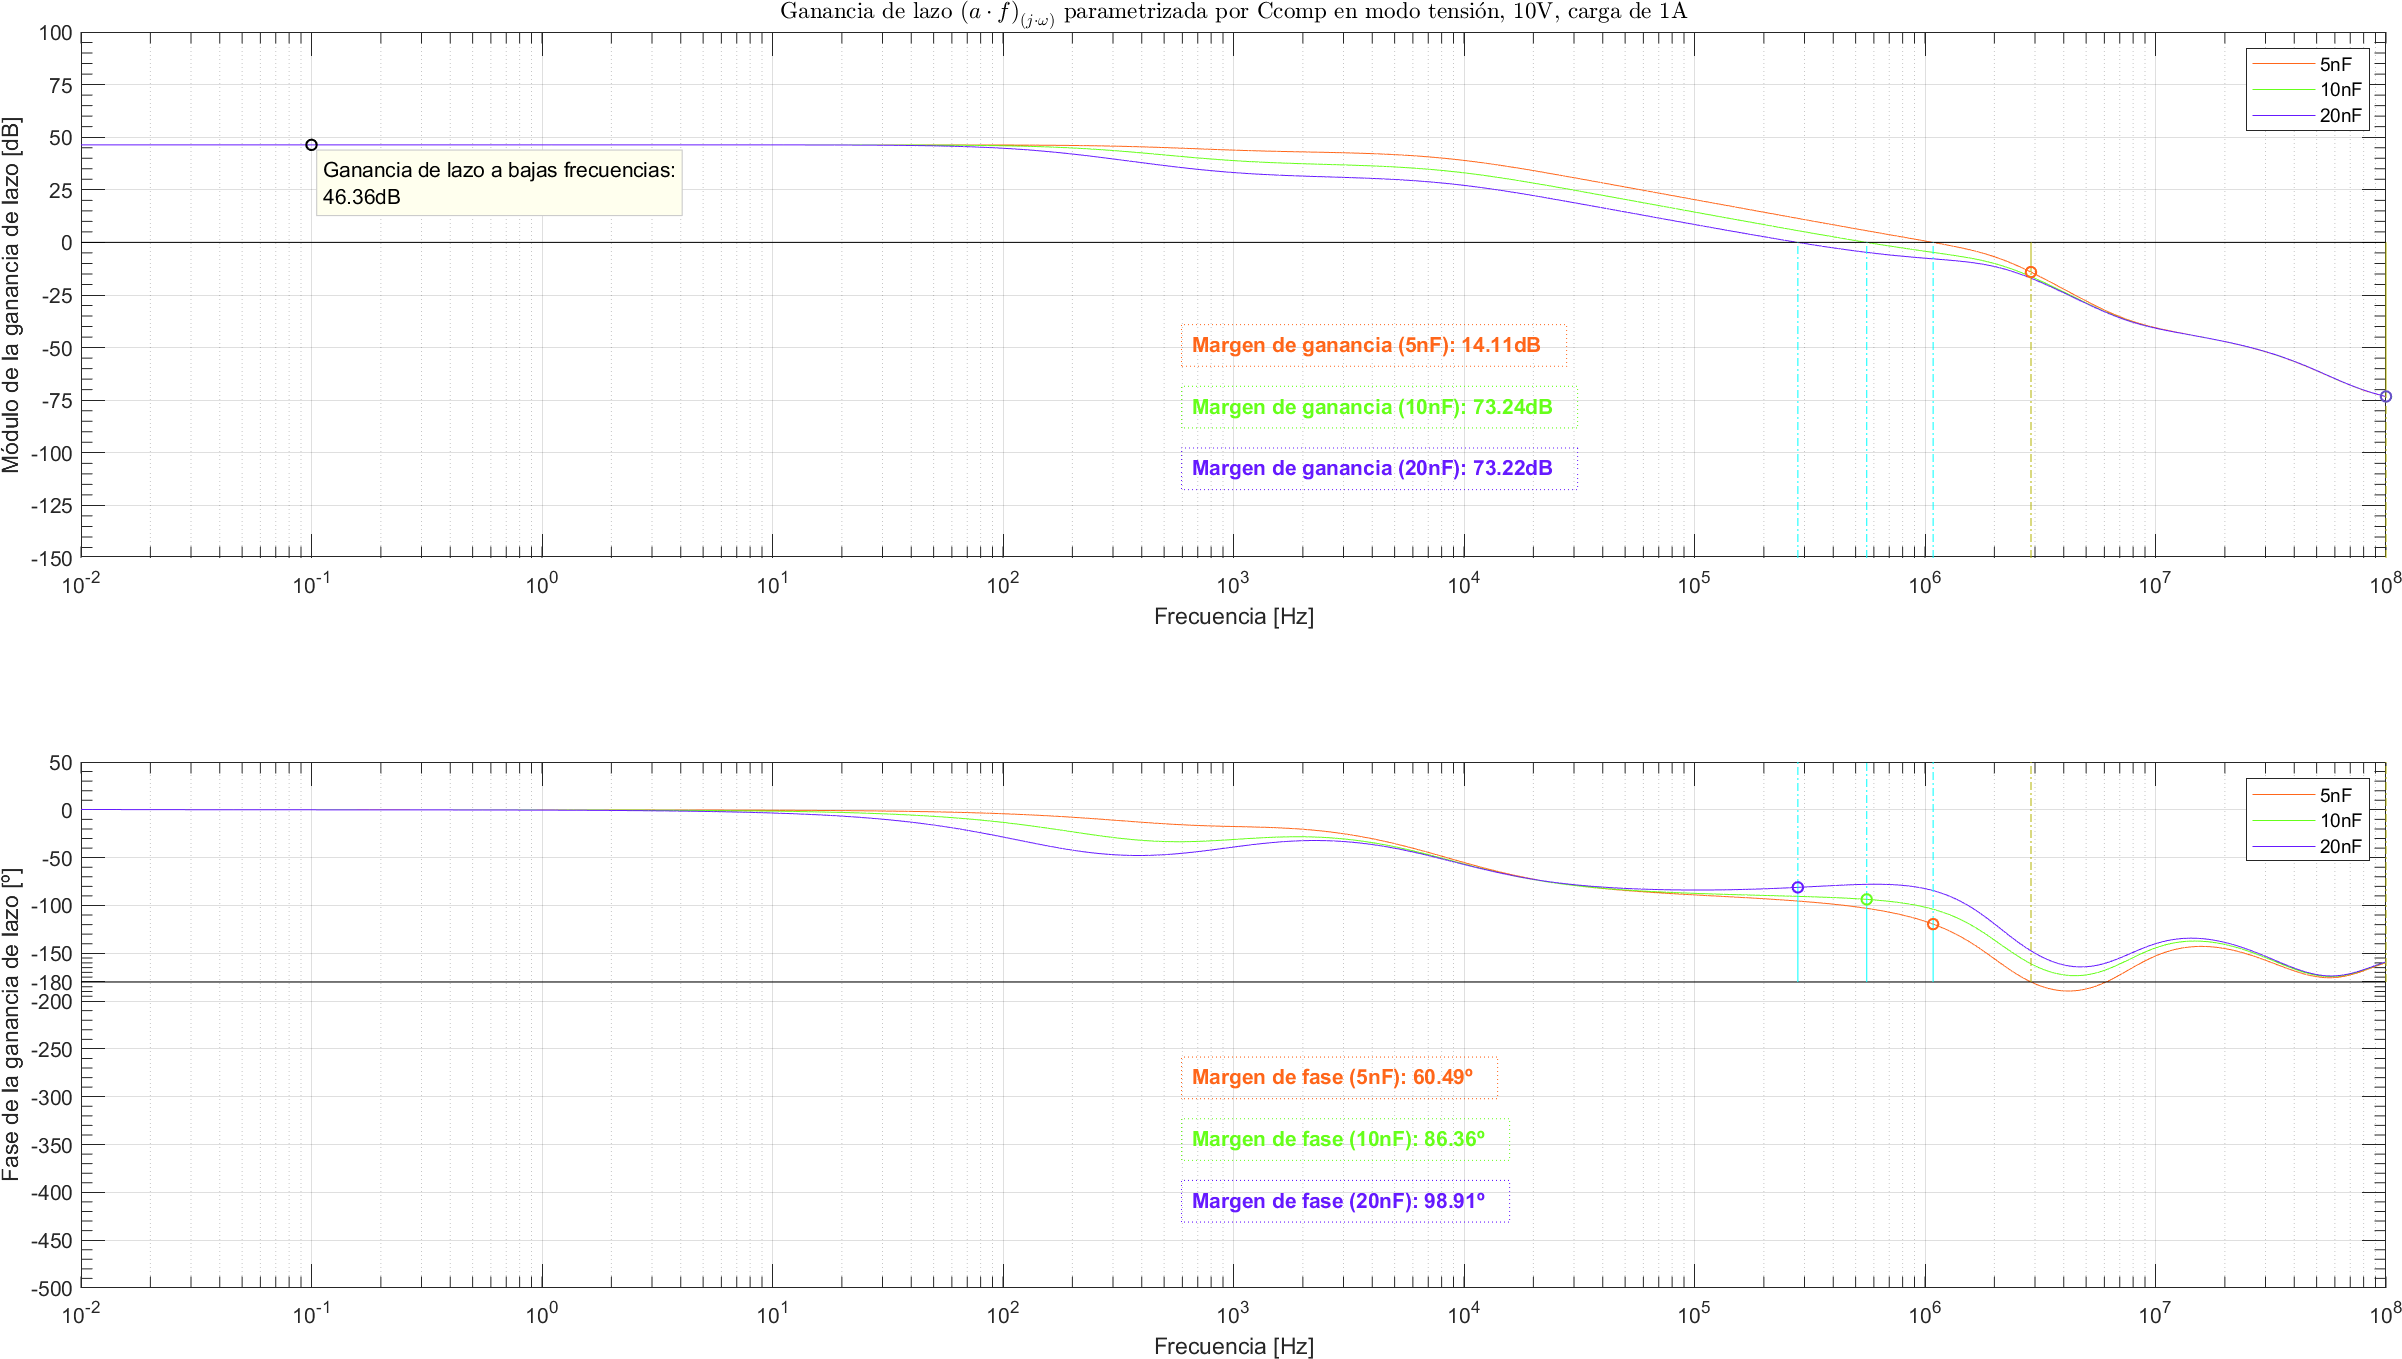
\includegraphics[width=1.1 \textwidth, angle=90]{./img/plots/loop/power_supply_CCOMP_LOOP_Modo1.png}
\caption{\label{fig:fig_power_supply_CCOMP_LOOP_Modo1}\footnotesize{Ganancia de lazo en función de la frecuencia parametrizada por Ccomp.}}
\end{center}
\end{figure}

\clearpage


\subsubsection{Análisis para $R_{comp}$ en modo tensión, $V_{out} = 10 \si[per-mode=symbol]{\volt}$, $R_{L} = 10 \si[per-mode=symbol]{\ohm}$}
% RCOMP MODO 1.

\clearpage

\begin{figure}[H] %htb
\begin{center}
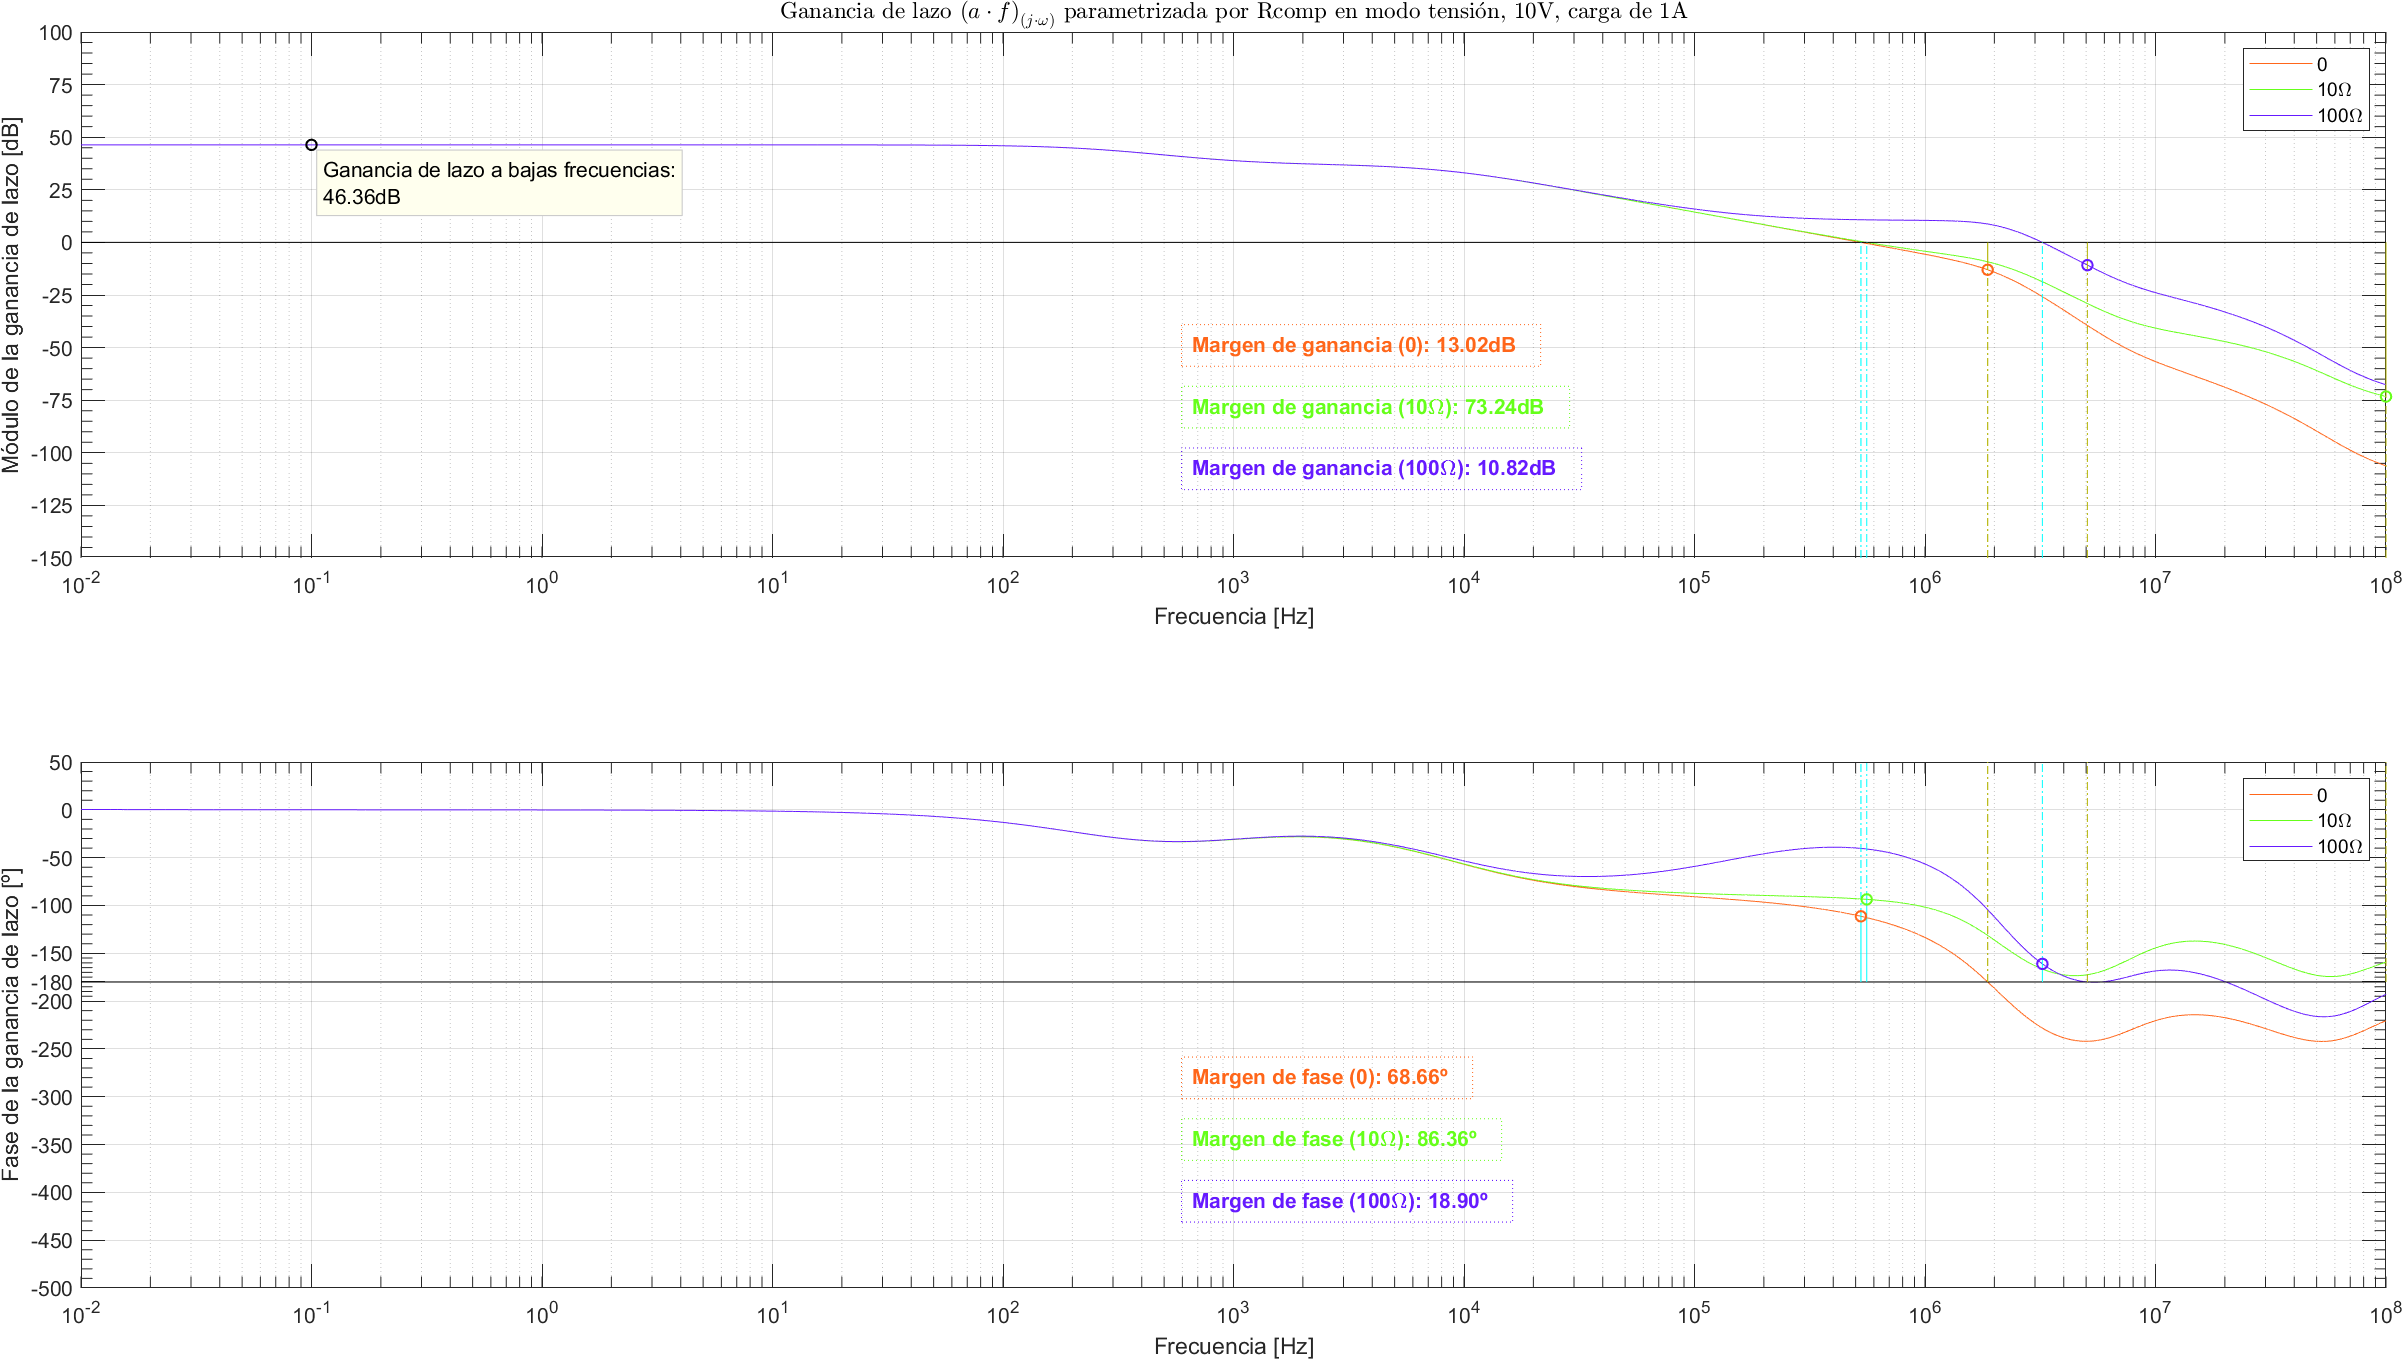
\includegraphics[width=1.1 \textwidth, angle=90]{./img/plots/loop/power_supply_RCOMP_LOOP_Modo1.png}
\caption{\label{fig:fig_power_supply_RCOMP_LOOP_Modo1}\footnotesize{Ganancia de lazo en modo tensión, $V_{out} = 10 \si[per-mode=symbol]{\volt}$, en función de la frecuencia parametrizada por $R_{comp}$.}}
\end{center}
\end{figure}


\clearpage

\begin{figure}[H] %htb
\begin{center}
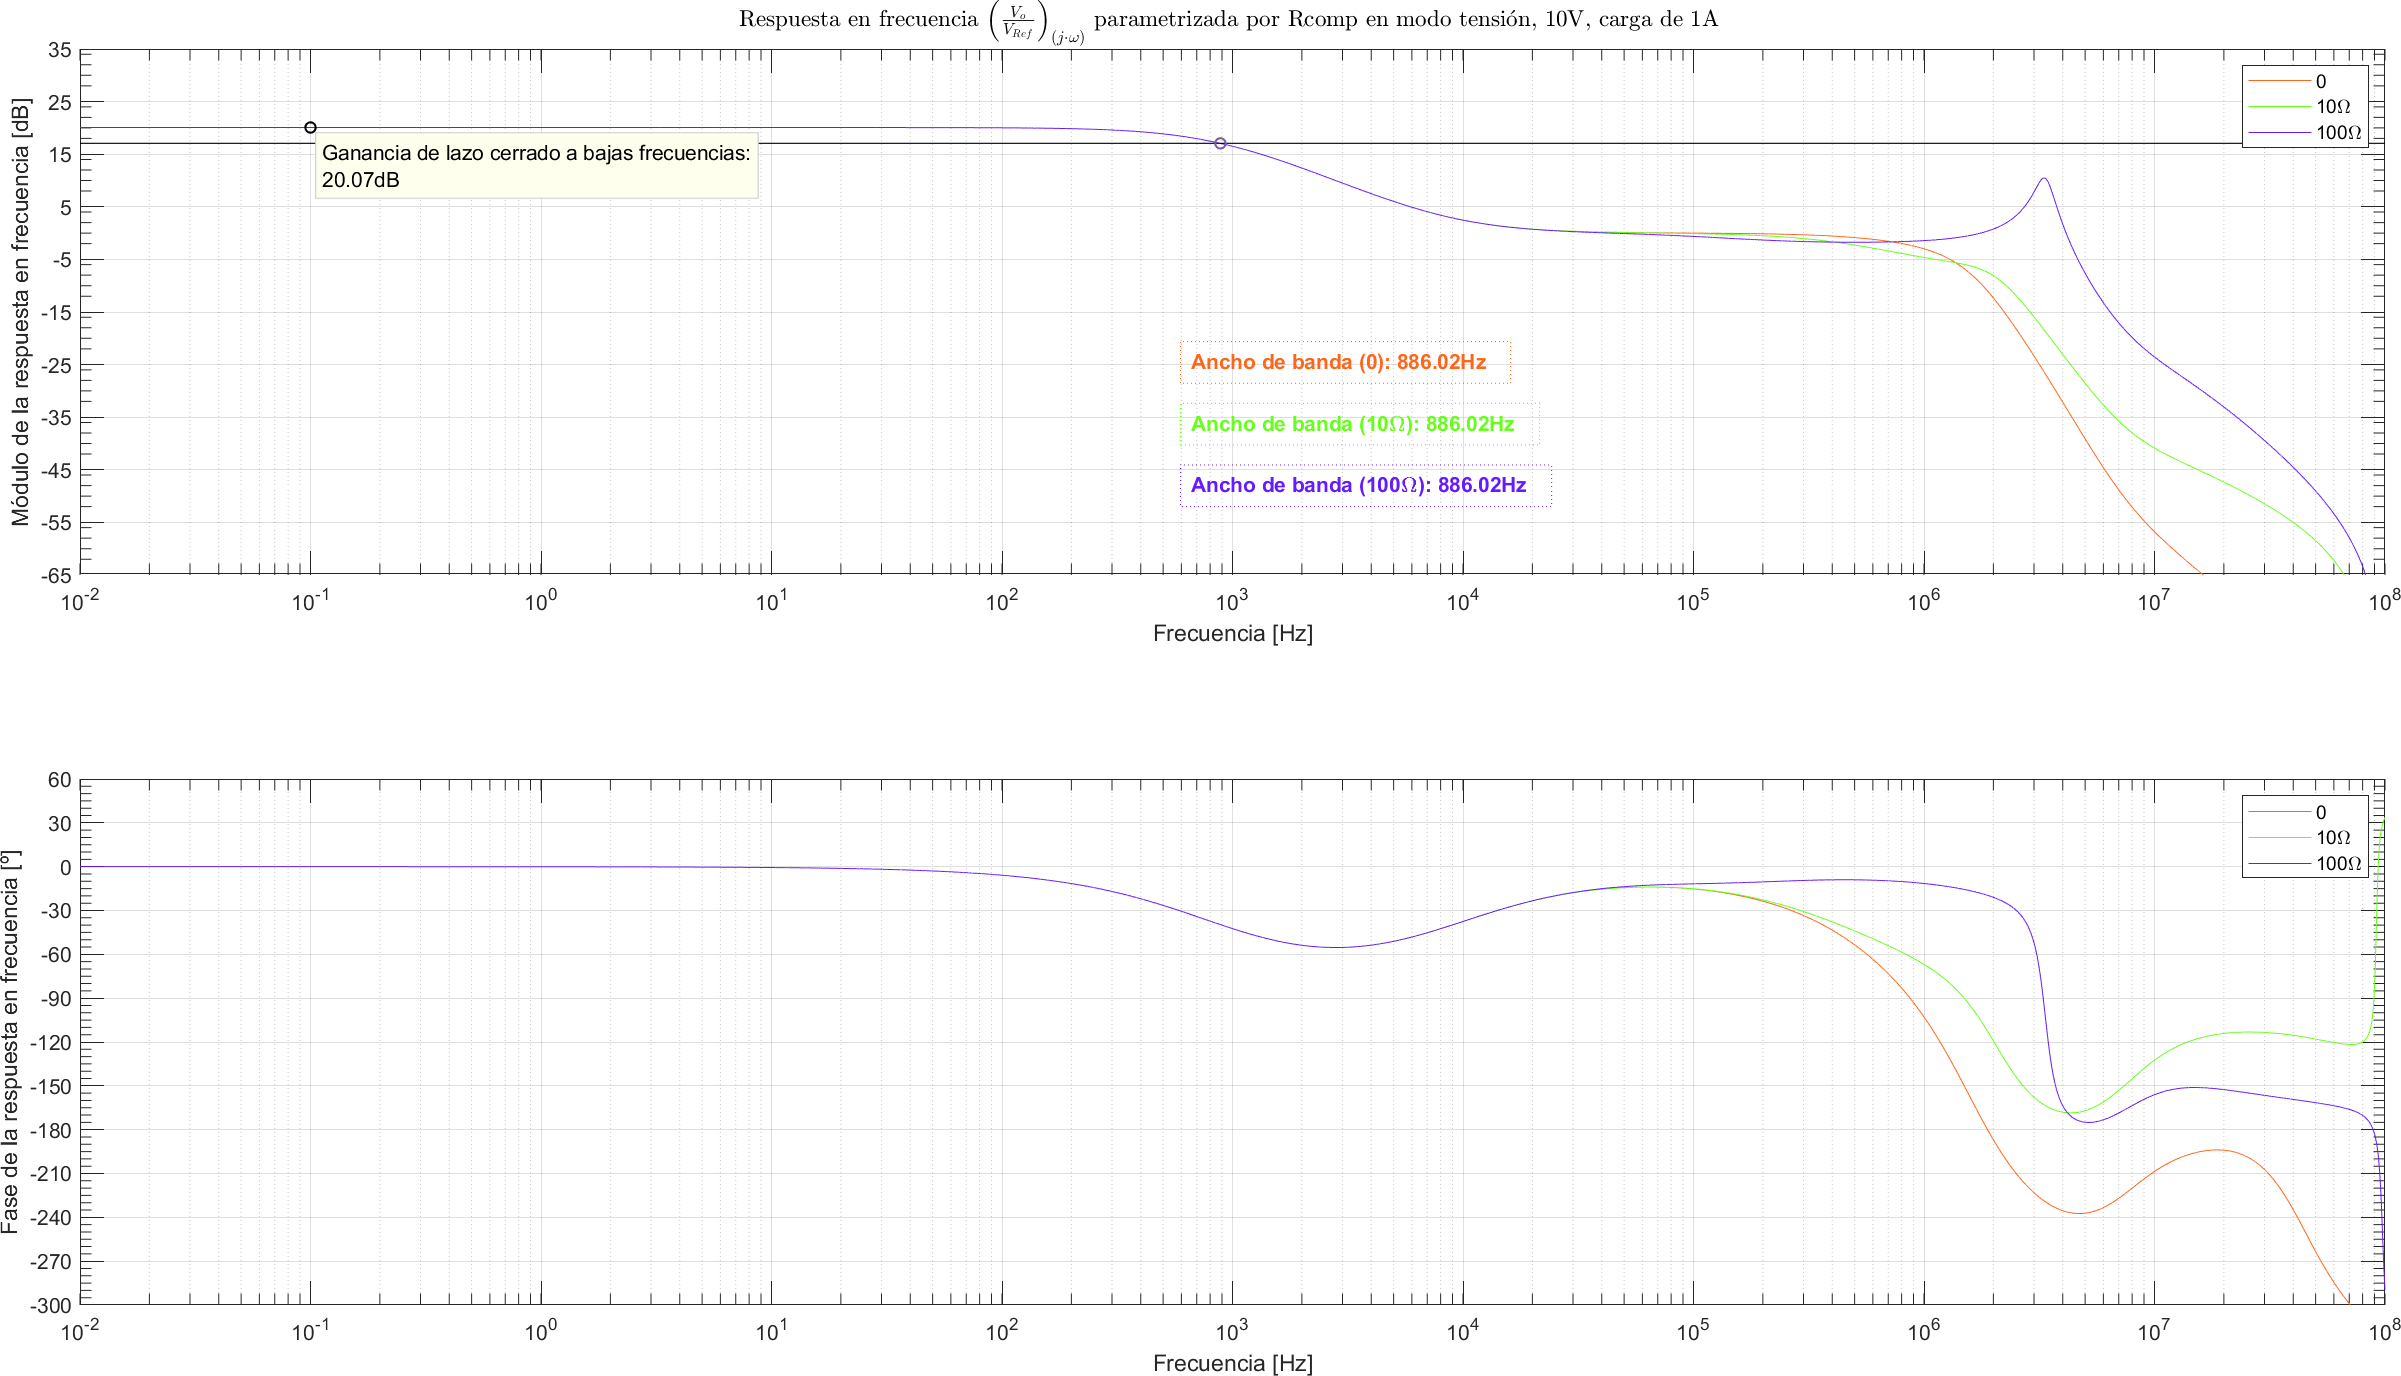
\includegraphics[width=1.1 \textwidth, angle=90]{./img/plots/rf/power_supply_RCOMP_RF_Modo1.png}
\caption{\label{fig:fig_power_supply_RCOMP_RF_Modo1}\footnotesize{Respuesta en frecuencia en modo tensión, $V_{out} = 10 \si[per-mode=symbol]{\volt}$, en función de la frecuencia parametrizada por $R_{comp}$.}}
\end{center}
\end{figure}

\clearpage

\begin{figure}[H] %htb
\begin{center}
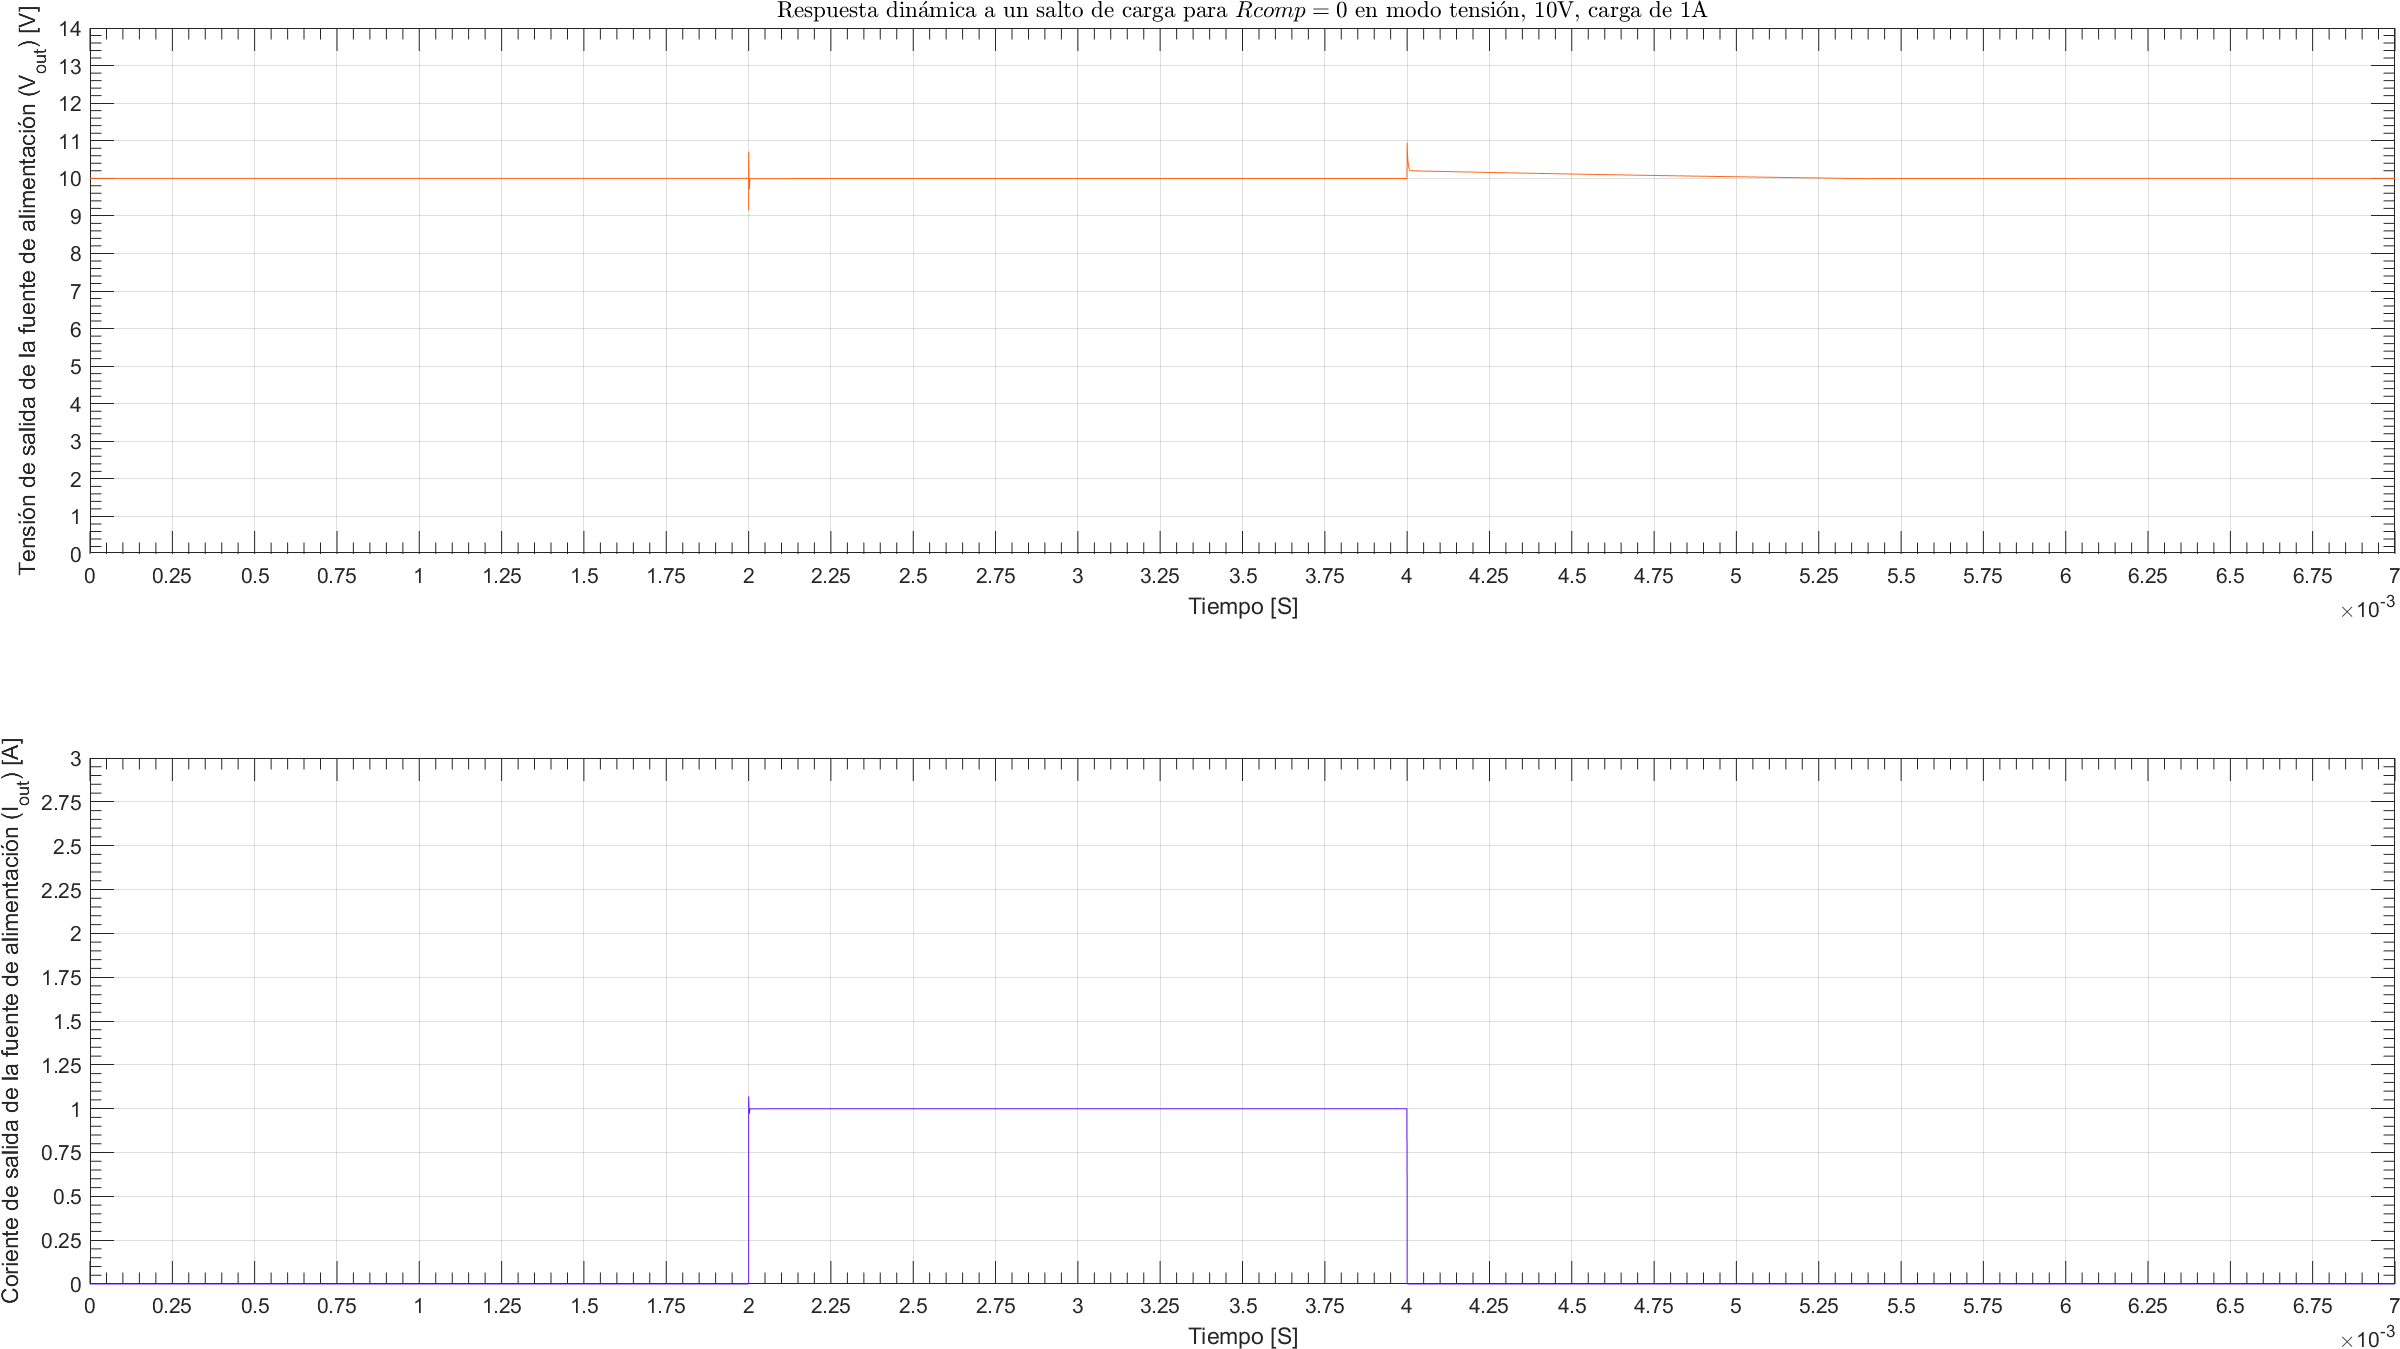
\includegraphics[width=1.1 \textwidth, angle=90]{./img/plots/dynamic/power_supply_RCOMP_0_STEP_Modo1.png}
\caption{\label{fig:fig_power_supply_RCOMP_STEP_5n_Modo1}\footnotesize{Respuesta dinámica en modo tensión, $V_{out} = 10 \si[per-mode=symbol]{\volt}$, para $R_{comp} = 0 \si[per-mode=symbol]{\ohm} $.}}
\end{center}
\end{figure}

\clearpage

\begin{figure}[H] %htb
\begin{center}
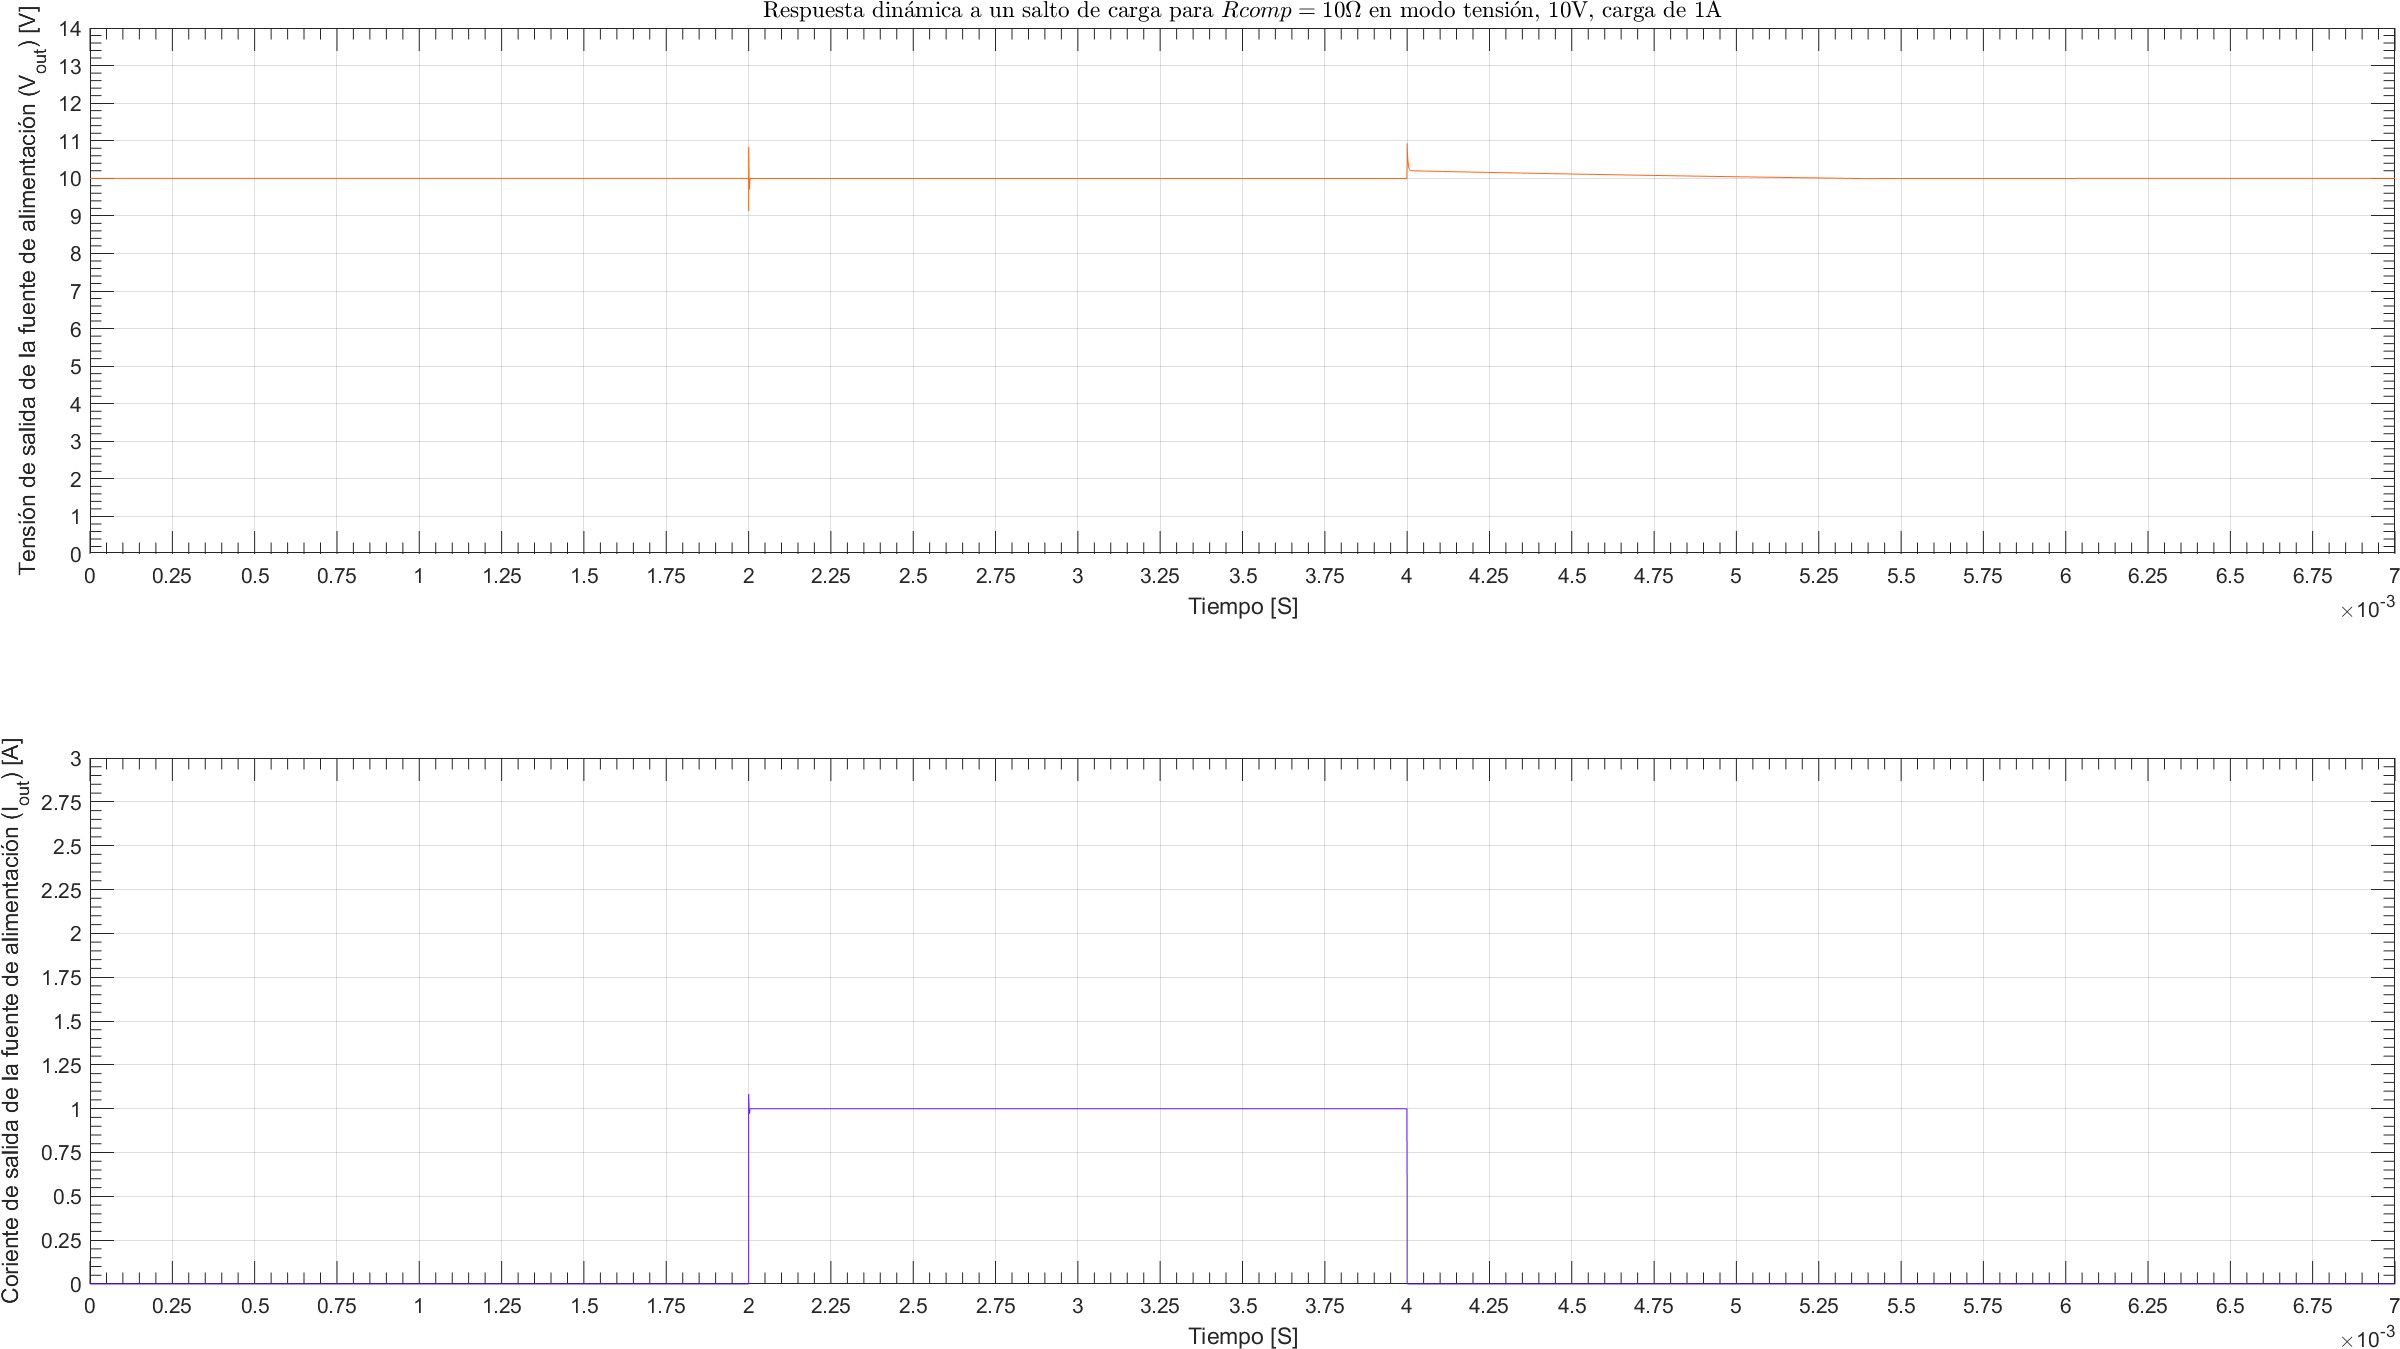
\includegraphics[width=1.1 \textwidth, angle=90]{./img/plots/dynamic/power_supply_RCOMP_10_STEP_Modo1.png}
\caption{\label{fig:fig_power_supply_RCOMP_STEP_10n_Modo1}\footnotesize{Respuesta dinámica en modo tensión, $V_{out} = 10 \si[per-mode=symbol]{\volt}$, para $R_{comp} = 10 \si[per-mode=symbol]{\ohm} $.}}
\end{center}
\end{figure}

\clearpage

\begin{figure}[H] %htb
\begin{center}
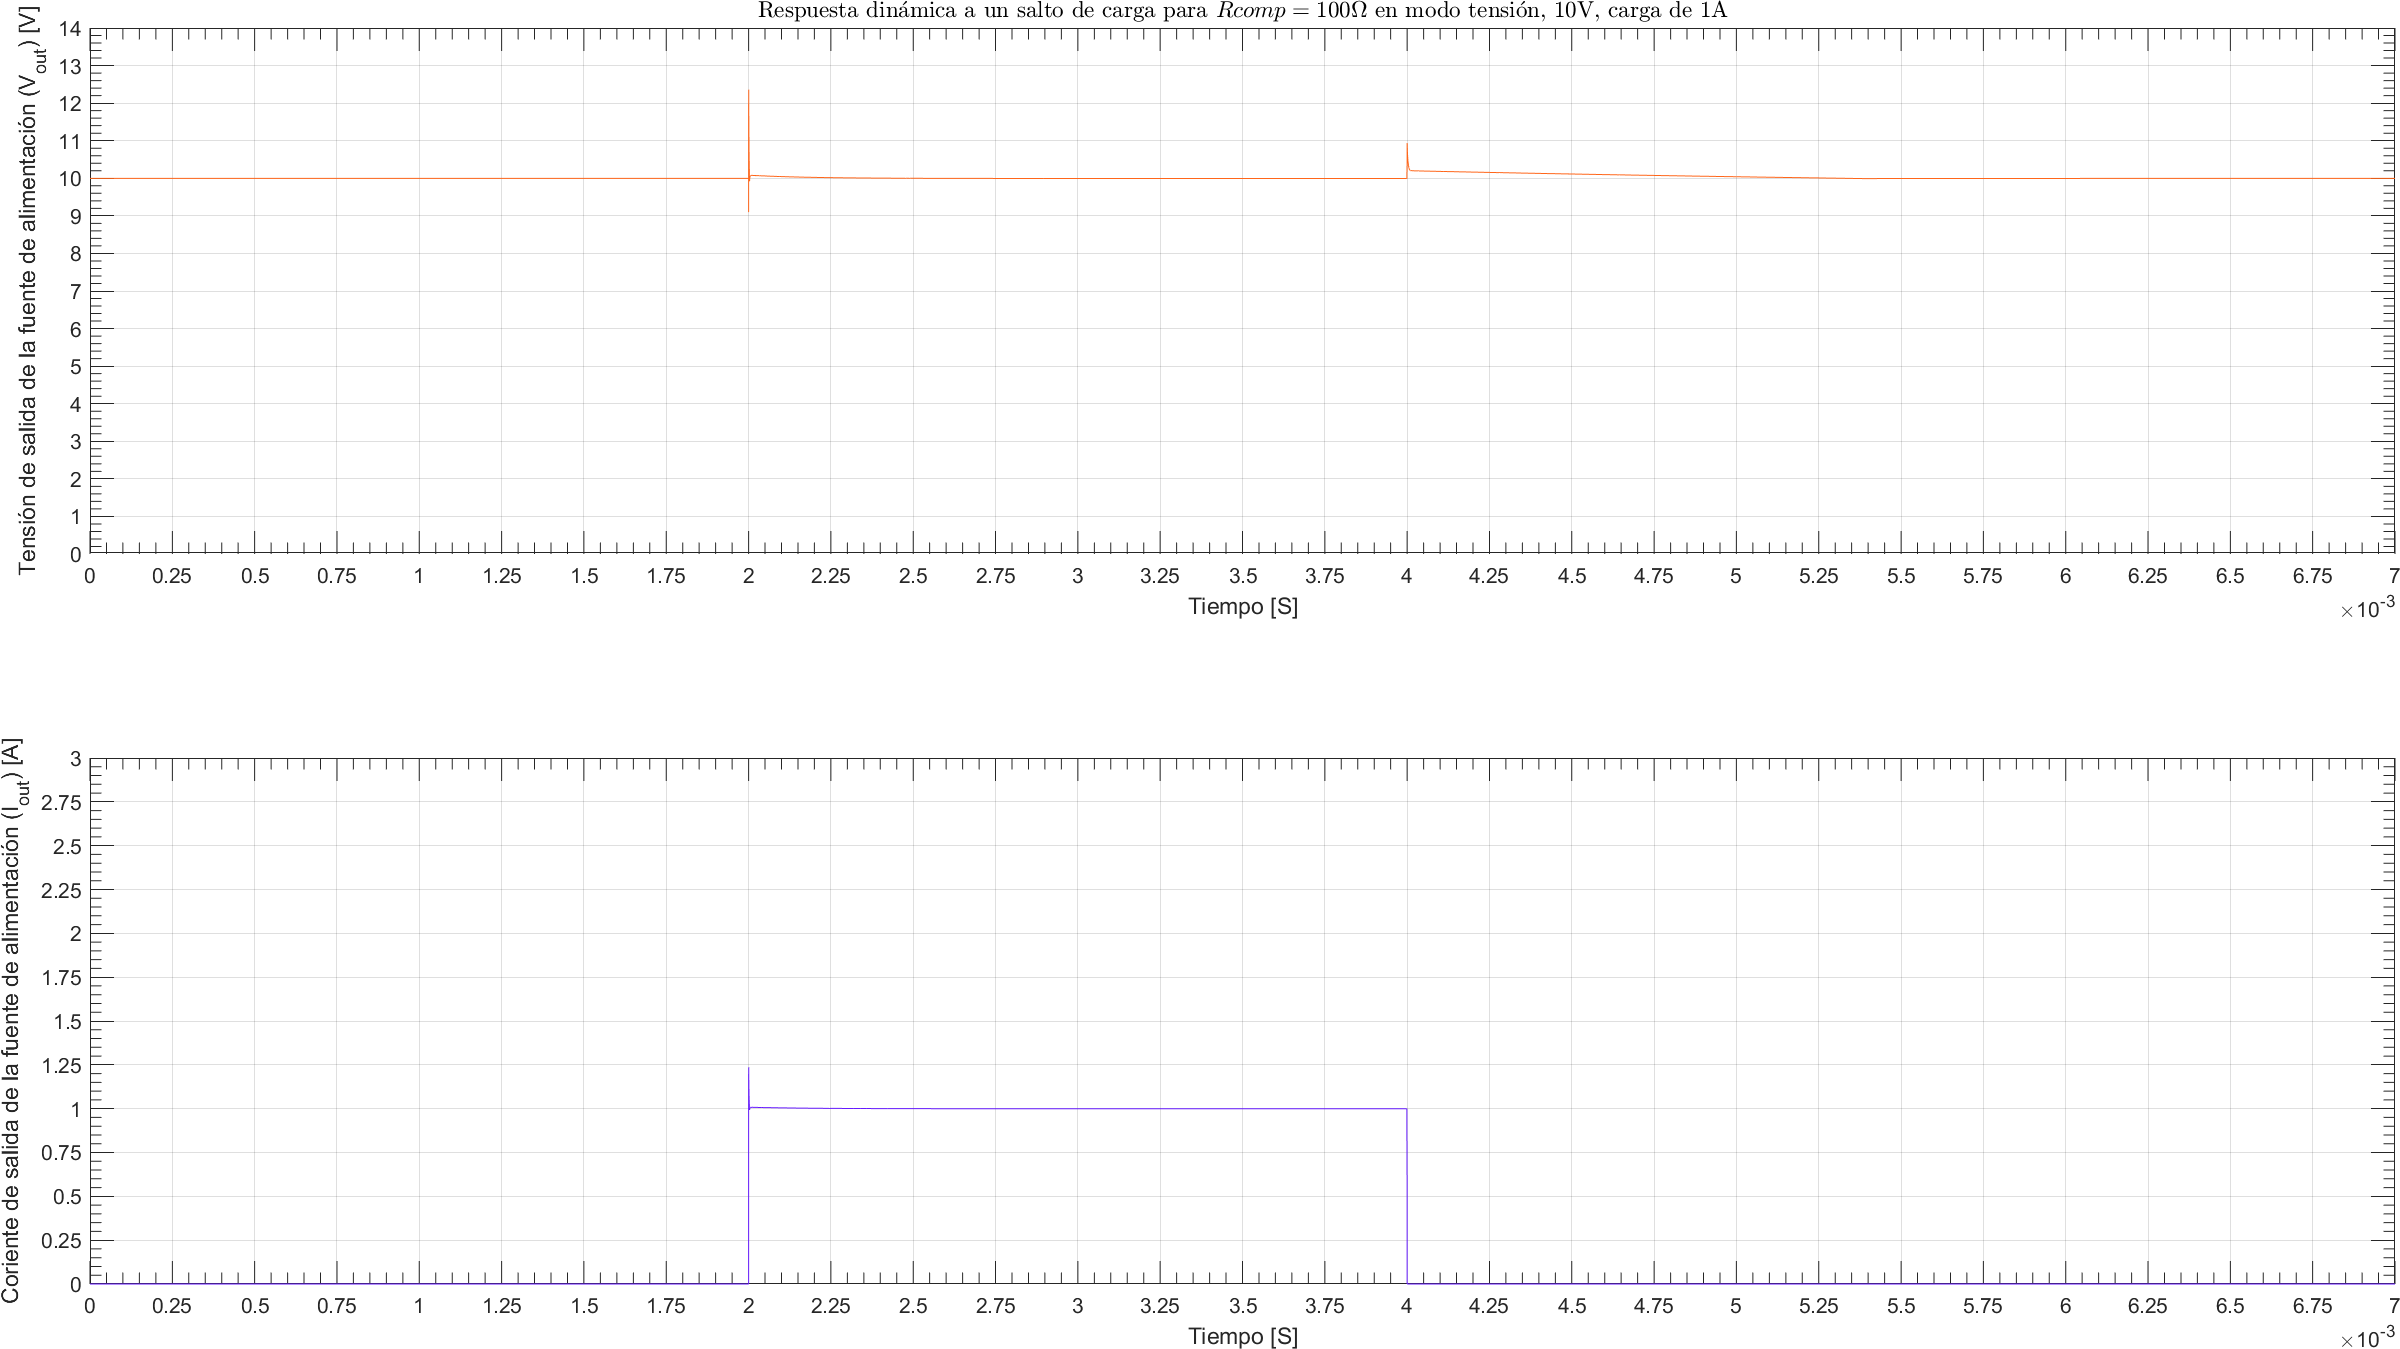
\includegraphics[width=1.1 \textwidth, angle=90]{./img/plots/dynamic/power_supply_RCOMP_100_STEP_Modo1.png}
\caption{\label{fig:fig_power_supply_RCOMP_STEP_20n_Modo1}\footnotesize{Respuesta dinámica en modo tensión, $V_{out} = 10 \si[per-mode=symbol]{\volt}$, para $R_{comp} = 100 \si[per-mode=symbol]{\ohm} $.}}
\end{center}
\end{figure}

\clearpage


\subsubsection{Análisis para $R_{comp}$ en modo tensión, $V_{out} = 1 \si[per-mode=symbol]{\volt}$, $R_{L} = 1 \si[per-mode=symbol]{\ohm}$}
% RCOMP MODO 2.

\clearpage

\begin{figure}[H] %htb
\begin{center}
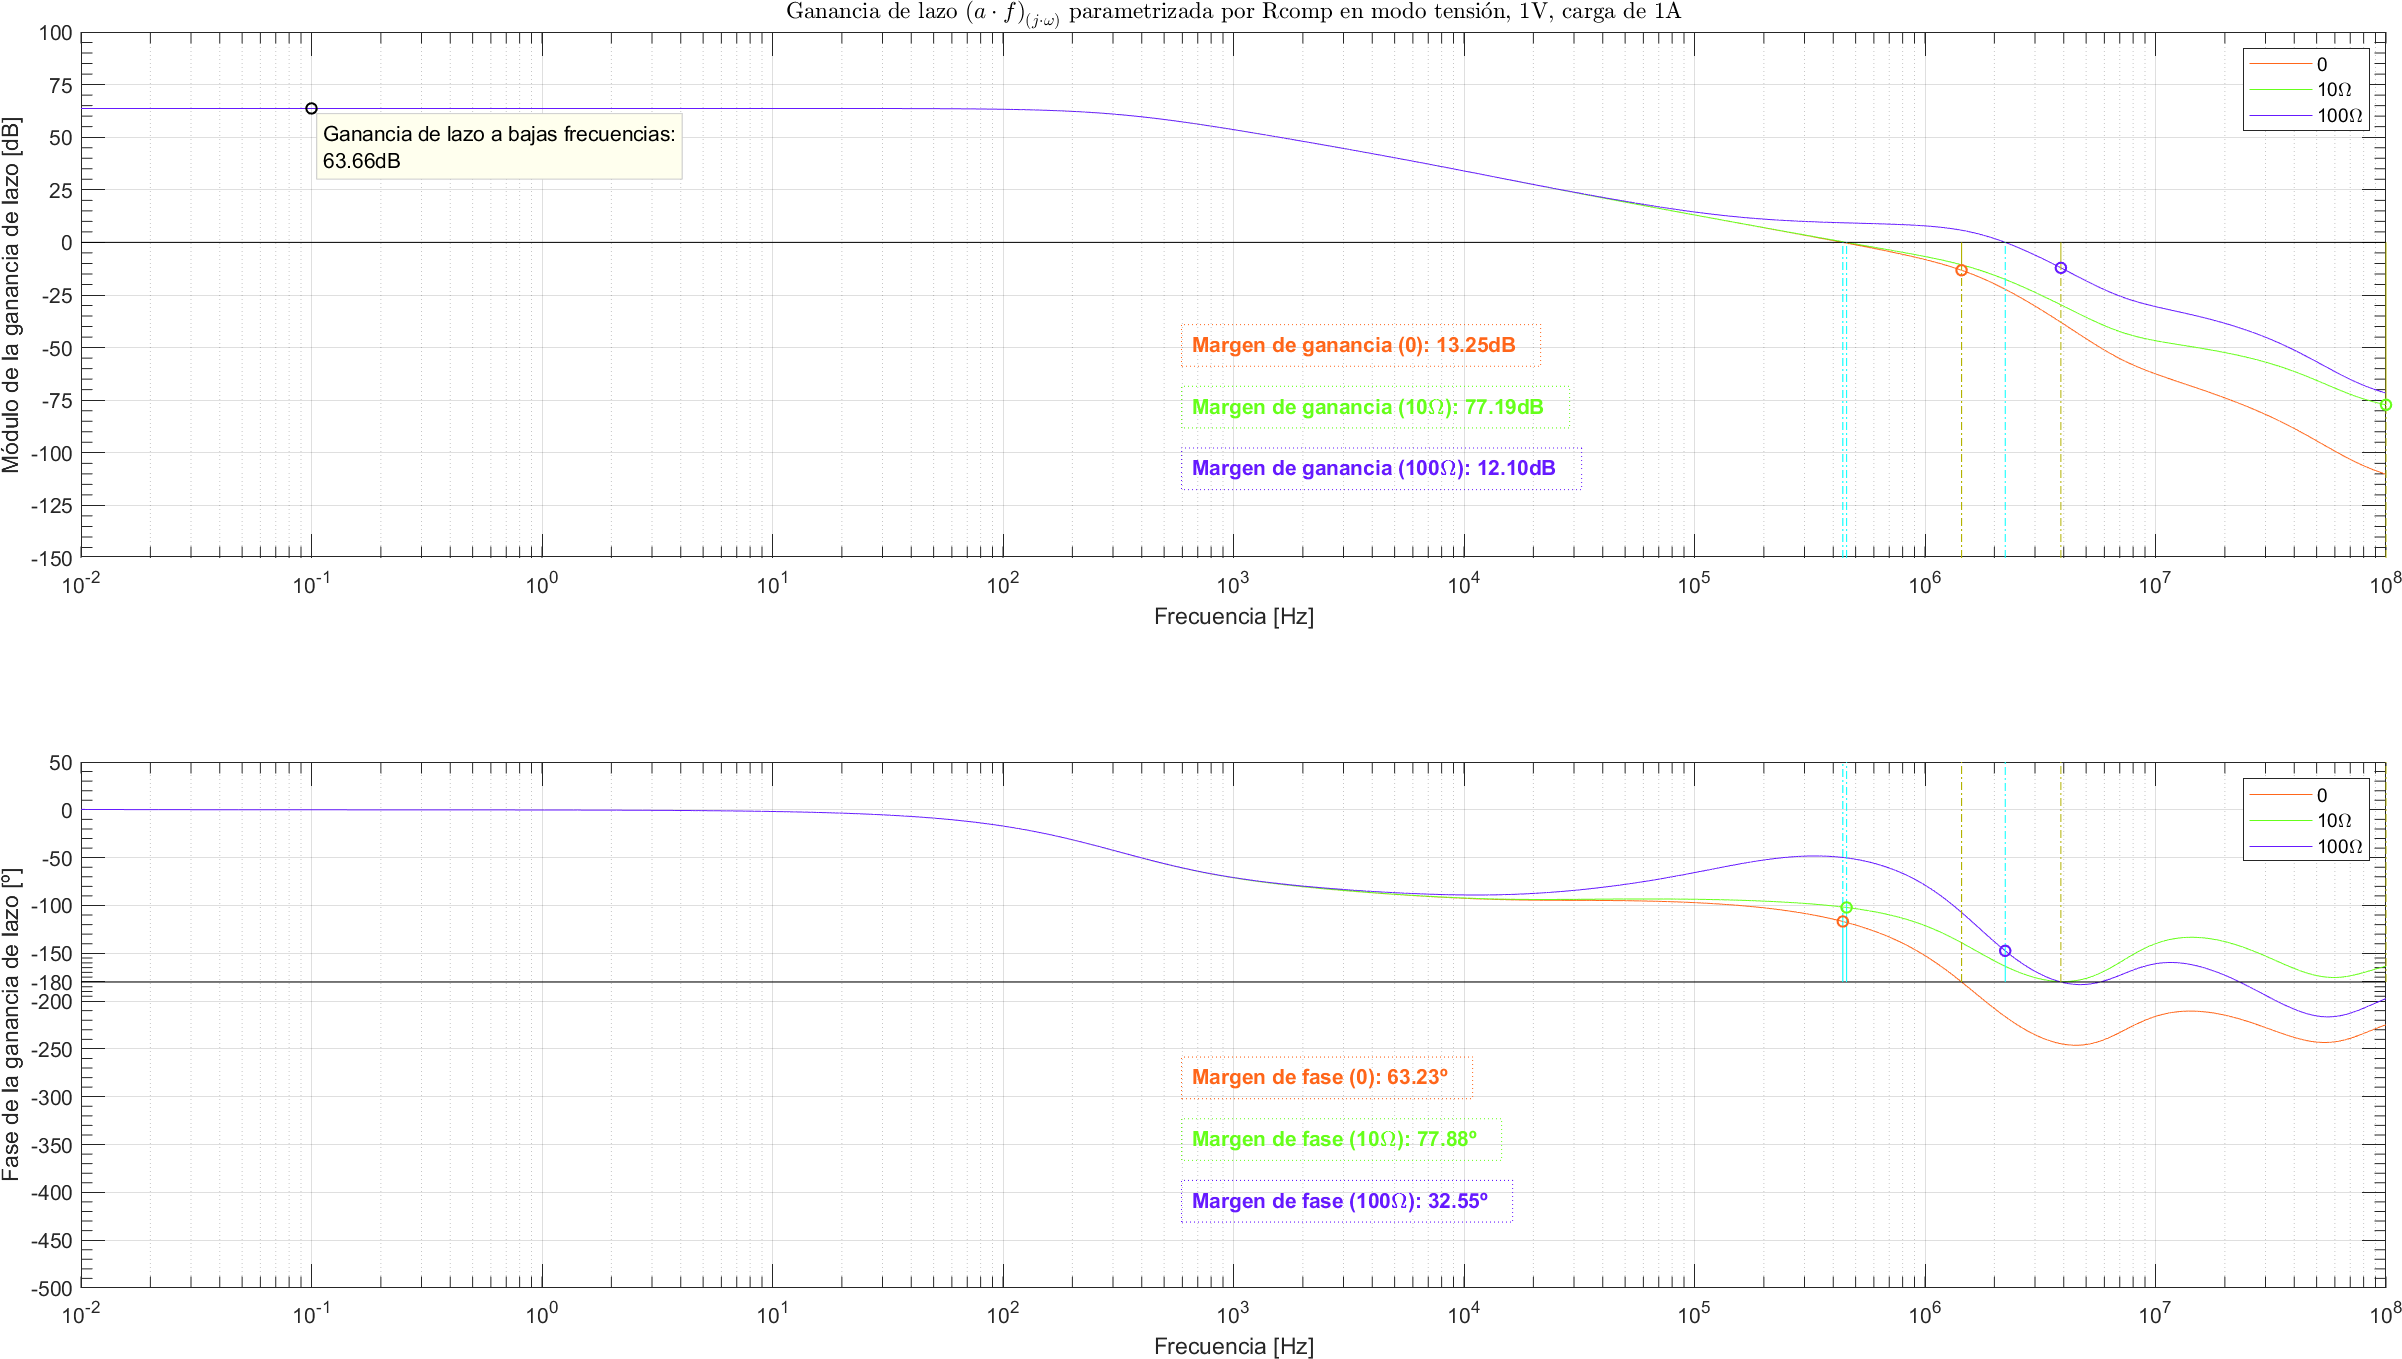
\includegraphics[width=1.1 \textwidth, angle=90]{./img/plots/loop/power_supply_RCOMP_LOOP_Modo2.png}
\caption{\label{fig:fig_power_supply_RCOMP_LOOP_Modo2}\footnotesize{Ganancia de lazo en modo tensión, $V_{out} = 1 \si[per-mode=symbol]{\volt}$, en función de la frecuencia parametrizada por $R_{comp}$.}}
\end{center}
\end{figure}


\clearpage

\begin{figure}[H] %htb
\begin{center}
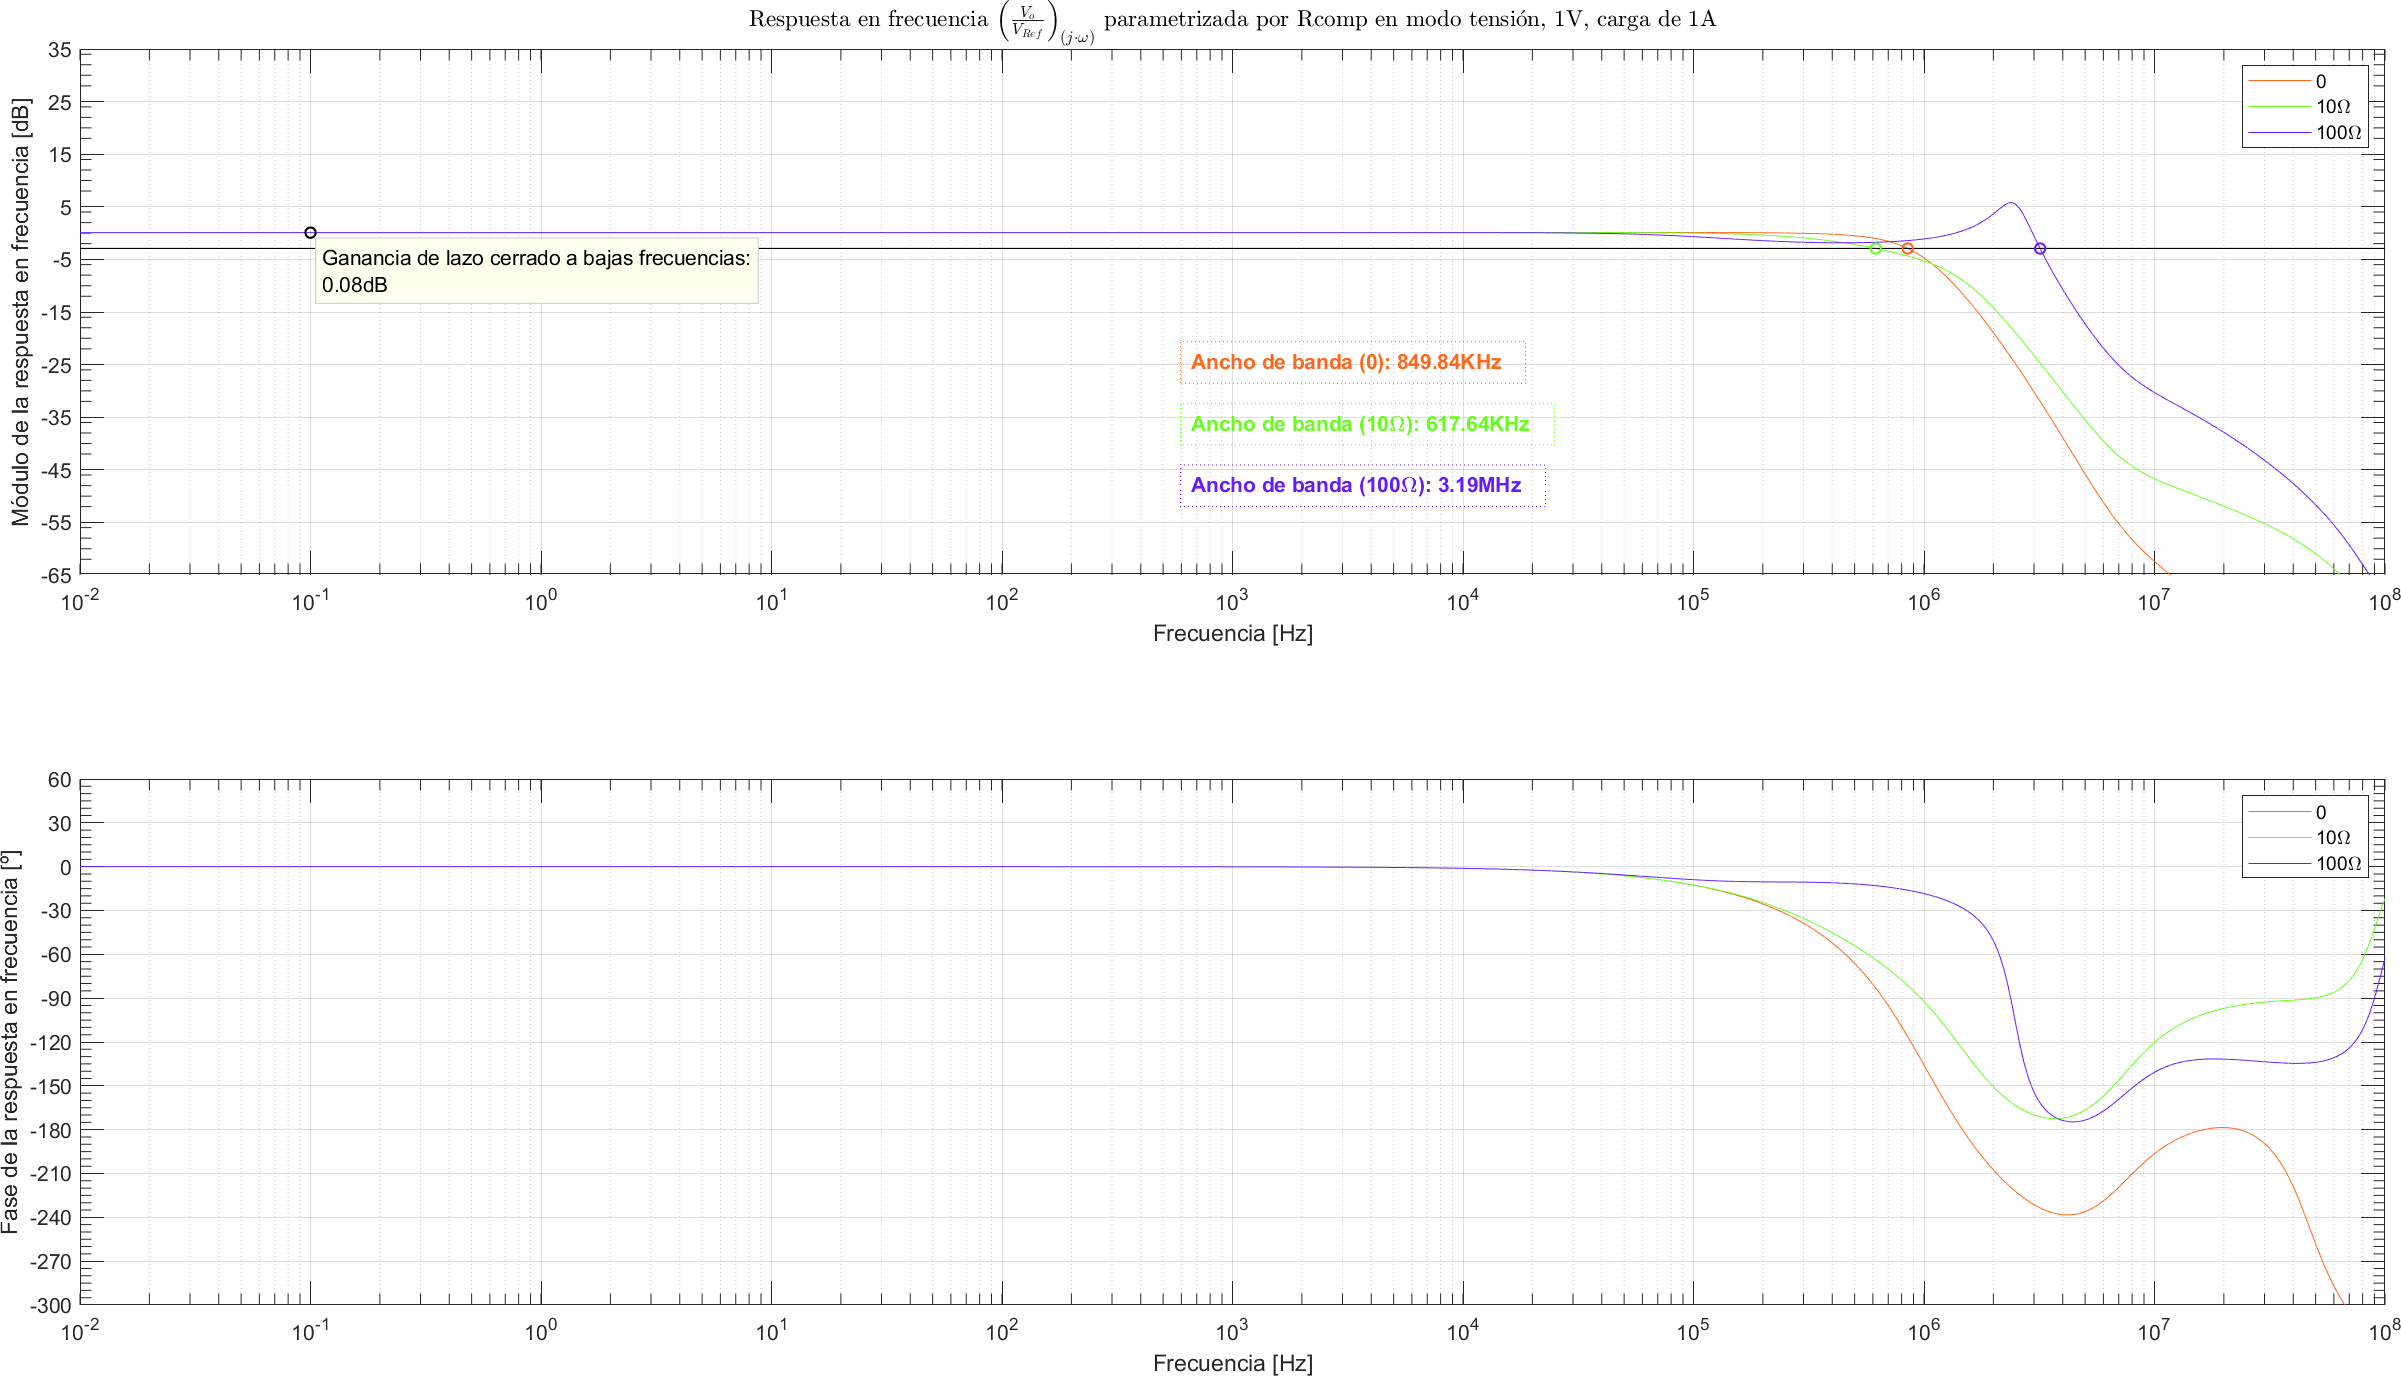
\includegraphics[width=1.1 \textwidth, angle=90]{./img/plots/rf/power_supply_RCOMP_RF_Modo2.png}
\caption{\label{fig:fig_power_supply_RCOMP_RF_Modo2}\footnotesize{Respuesta en frecuencia en modo tensión, $V_{out} = 1 \si[per-mode=symbol]{\volt}$, en función de la frecuencia parametrizada por $R_{comp}$.}}
\end{center}
\end{figure}

\clearpage

\begin{figure}[H] %htb
\begin{center}
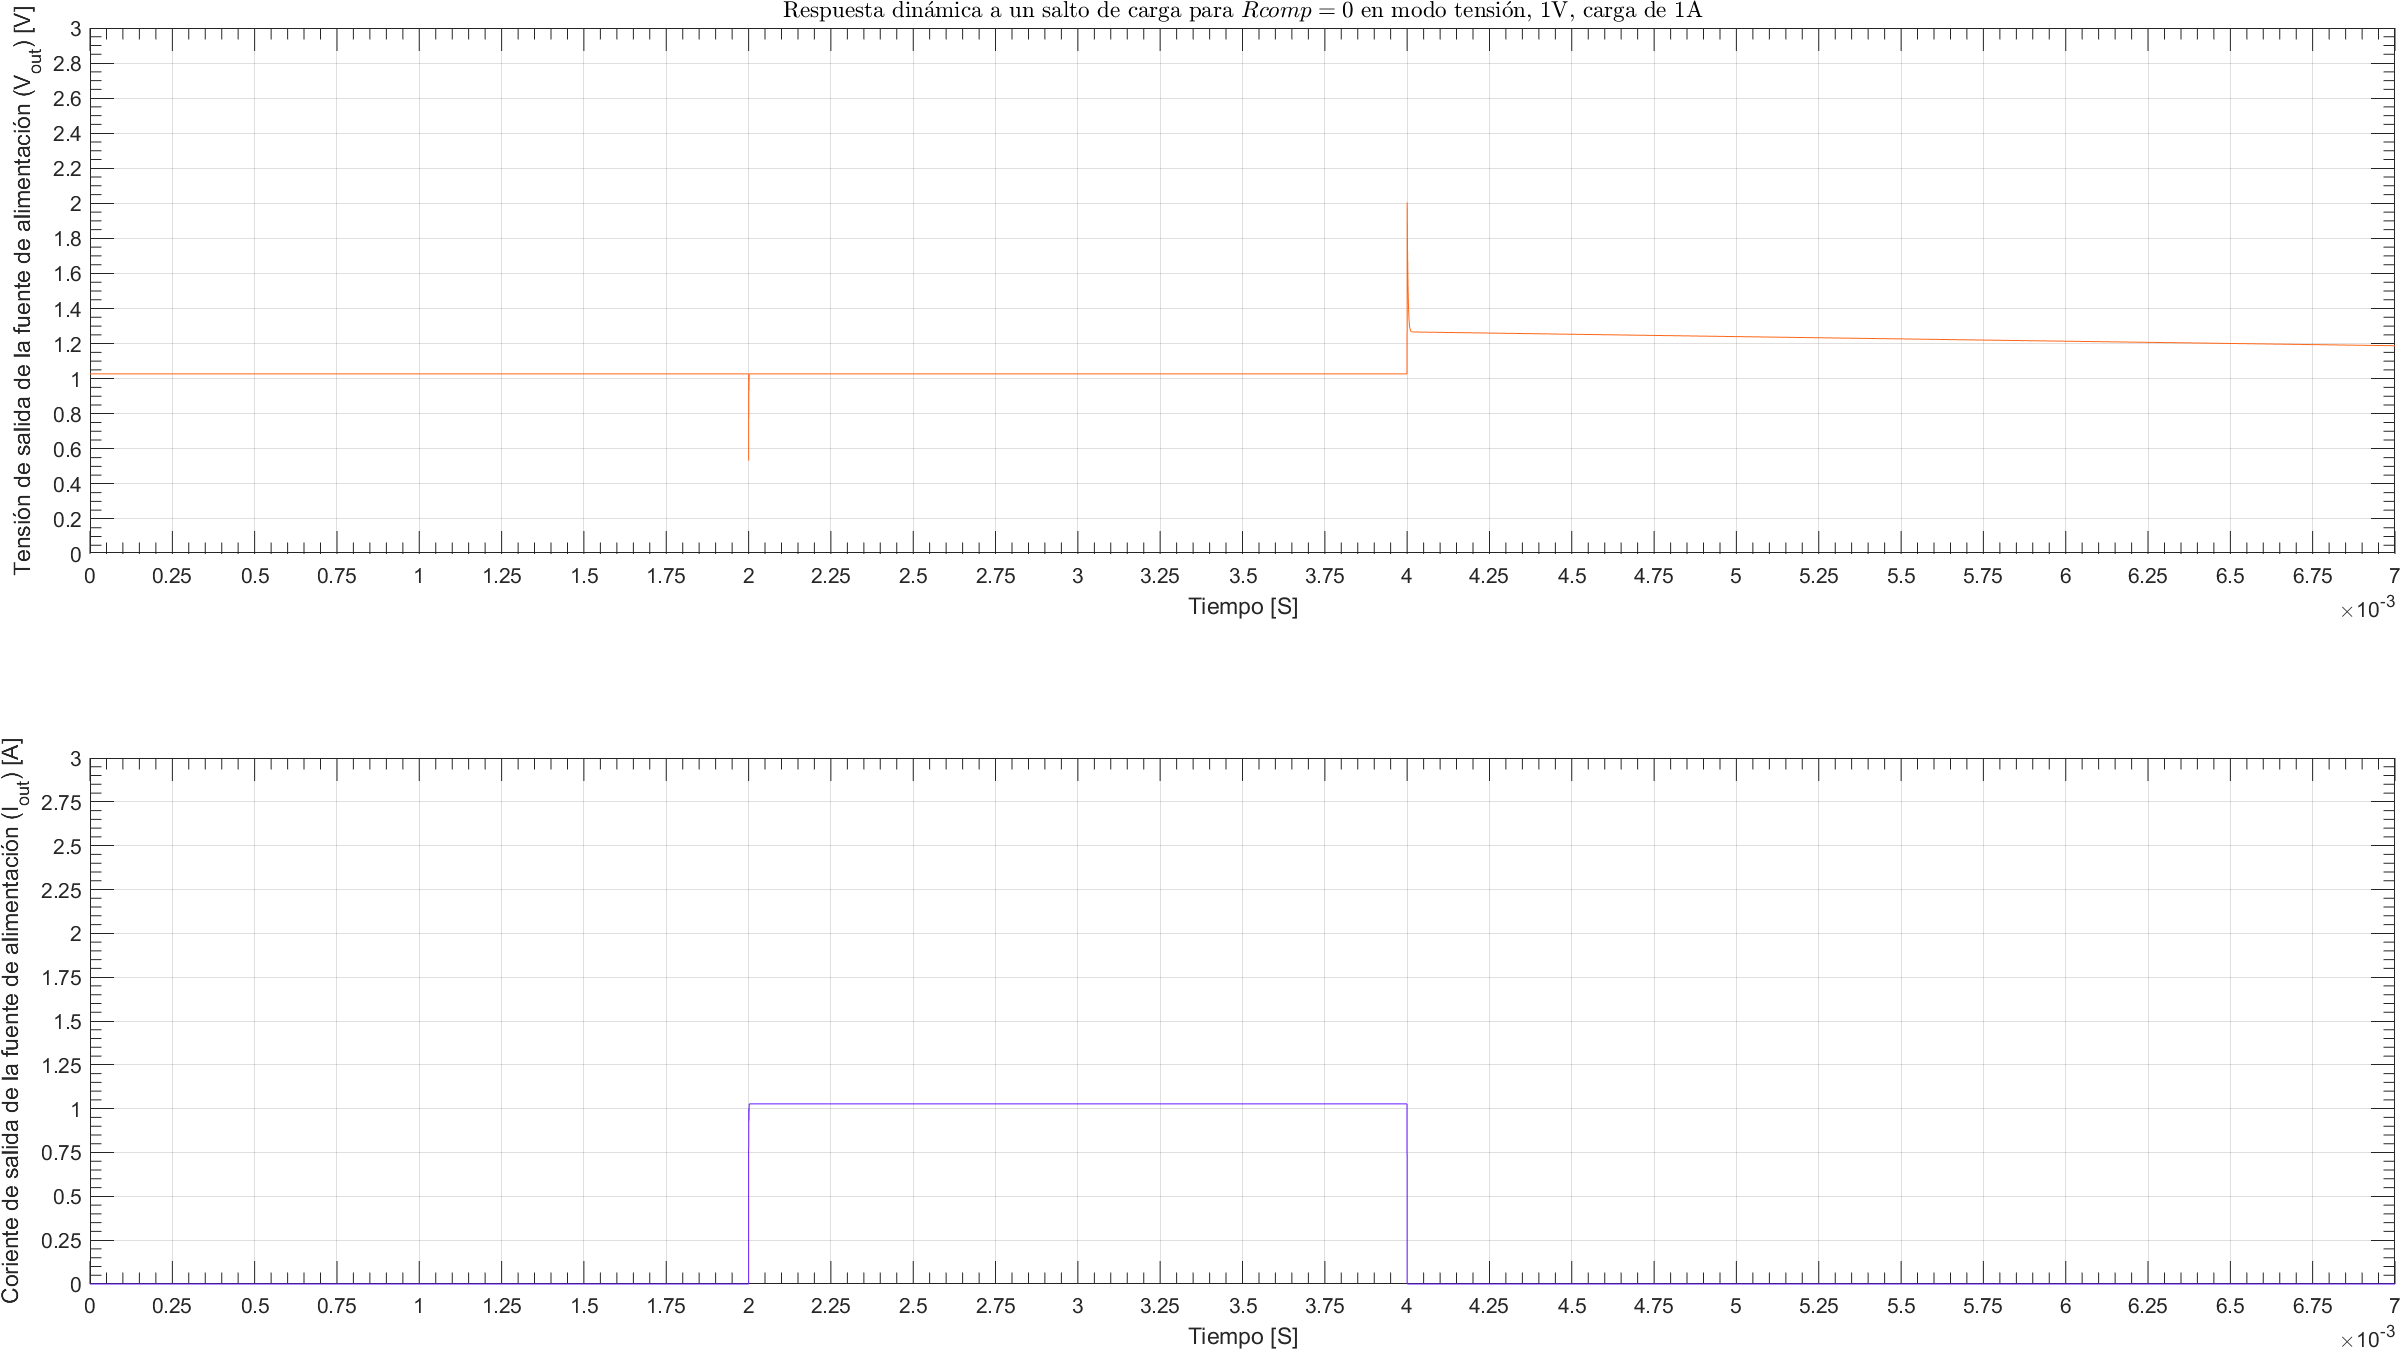
\includegraphics[width=1.1 \textwidth, angle=90]{./img/plots/dynamic/power_supply_RCOMP_0_STEP_Modo2.png}
\caption{\label{fig:fig_power_supply_RCOMP_STEP_5n_Modo2}\footnotesize{Respuesta dinámica en modo tensión, $V_{out} = 1 \si[per-mode=symbol]{\volt}$, para $R_{comp} = 0 \si[per-mode=symbol]{\ohm} $.}}
\end{center}
\end{figure}

\clearpage

\begin{figure}[H] %htb
\begin{center}
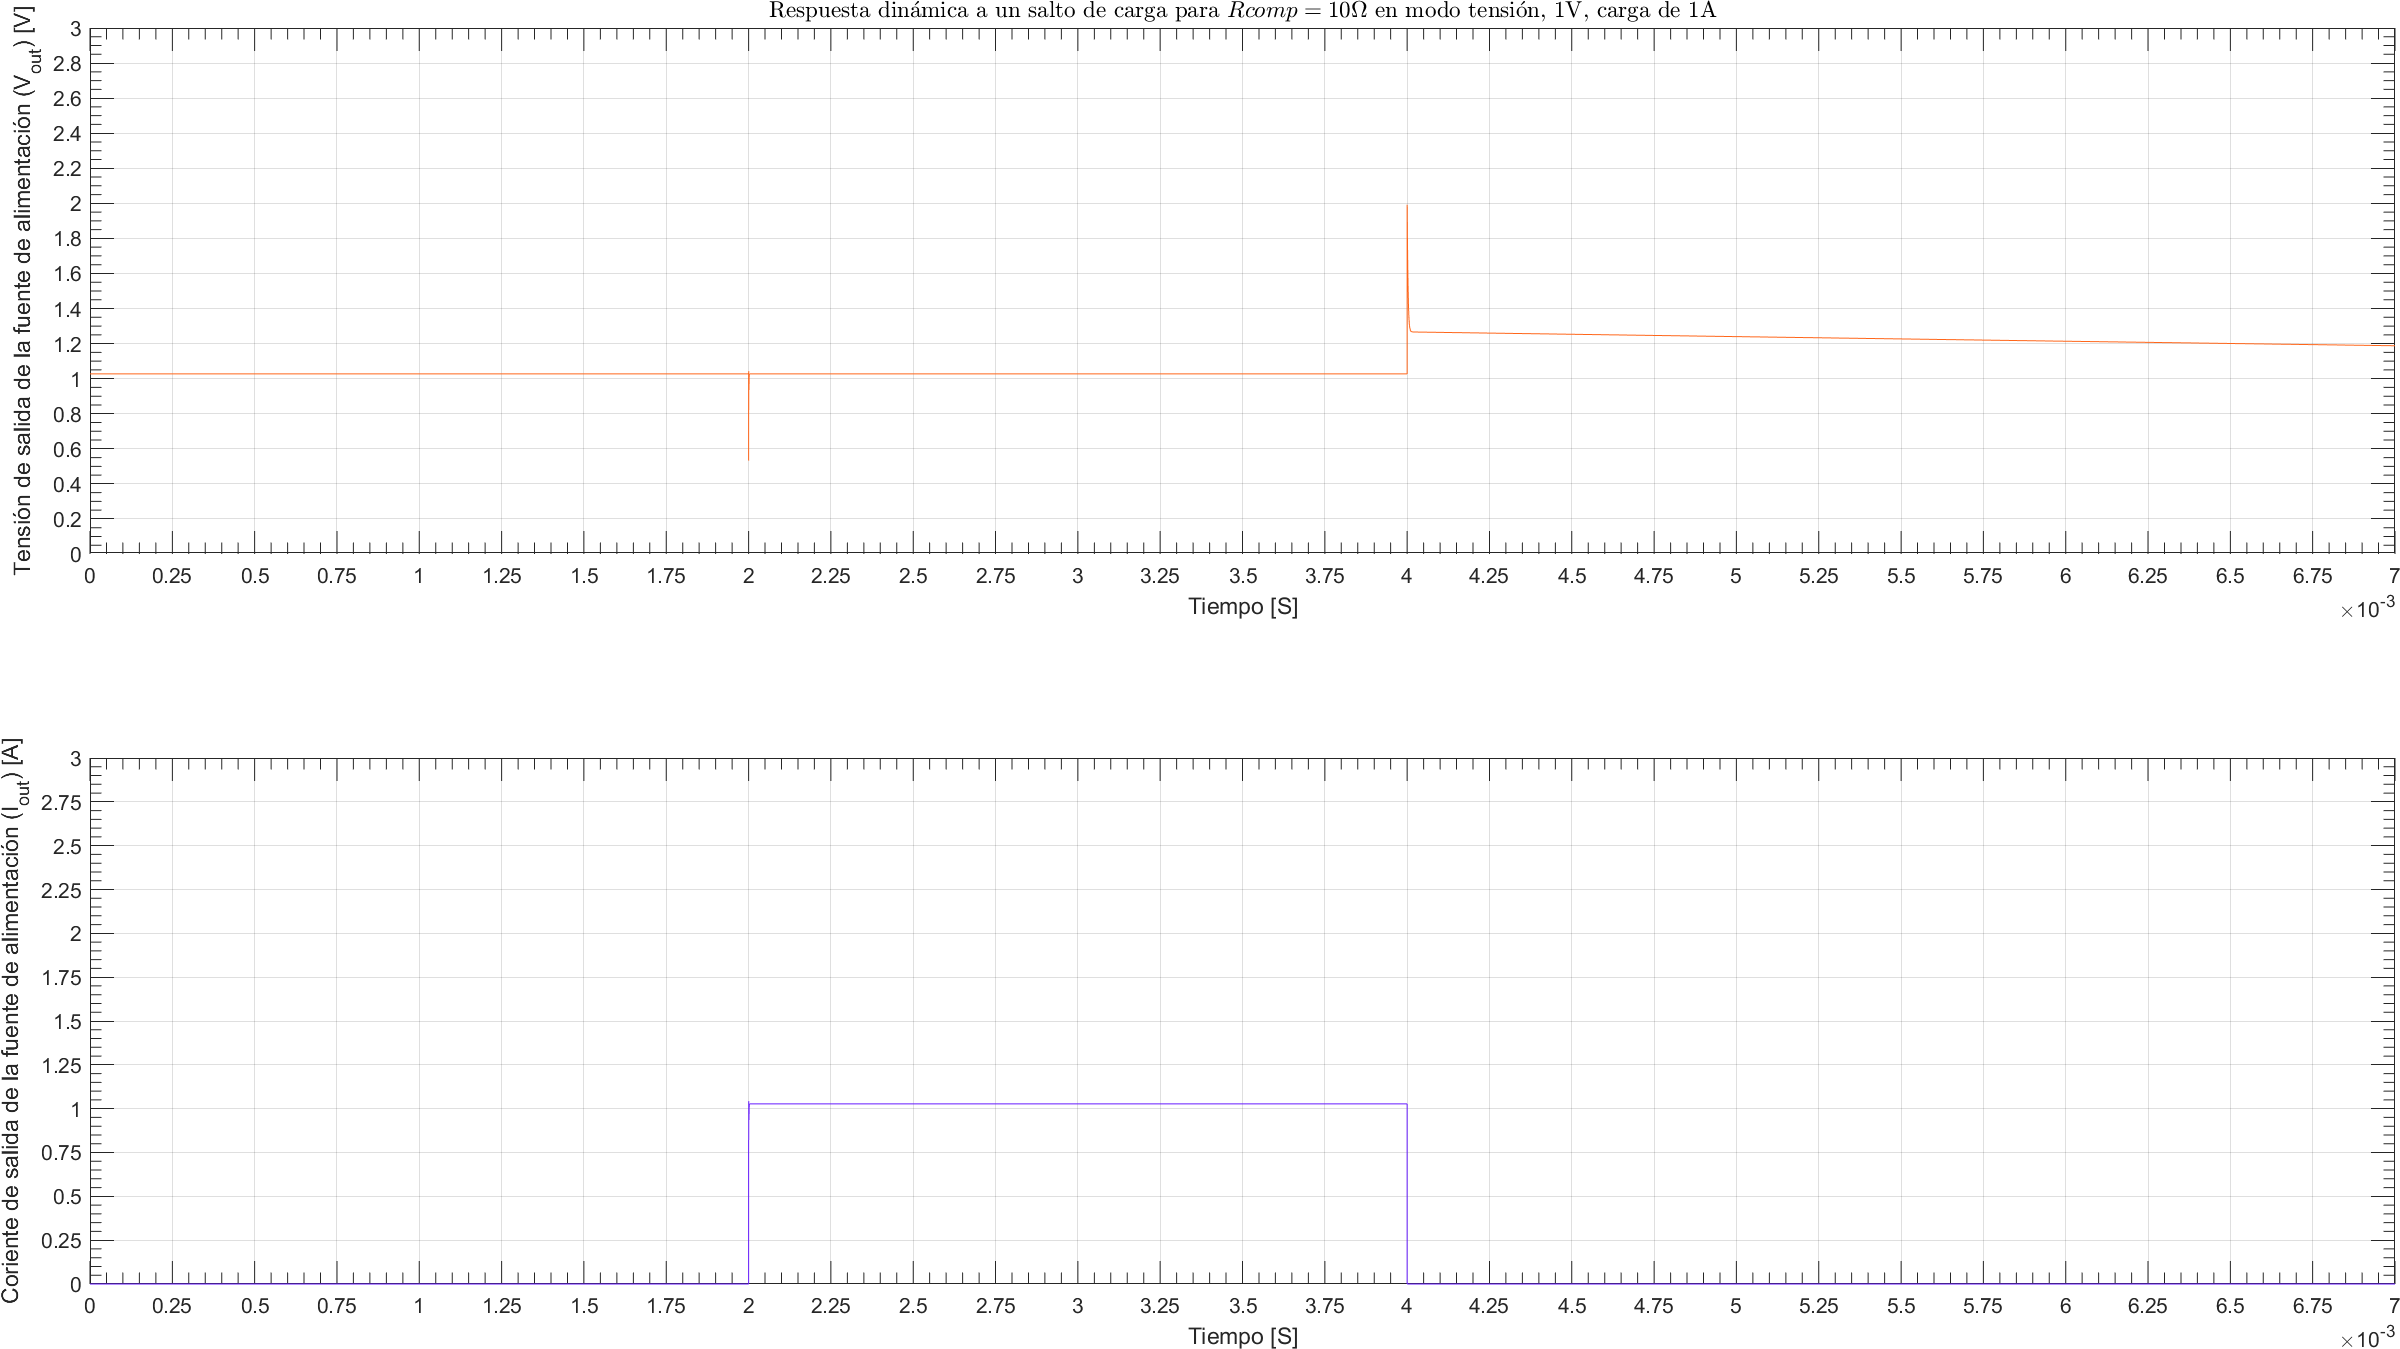
\includegraphics[width=1.1 \textwidth, angle=90]{./img/plots/dynamic/power_supply_RCOMP_10_STEP_Modo2.png}
\caption{\label{fig:fig_power_supply_RCOMP_STEP_10n_Modo2}\footnotesize{Respuesta dinámica en modo tensión, $V_{out} = 1 \si[per-mode=symbol]{\volt}$, para $R_{comp} = 10 \si[per-mode=symbol]{\ohm} $.}}
\end{center}
\end{figure}

\clearpage

\begin{figure}[H] %htb
\begin{center}
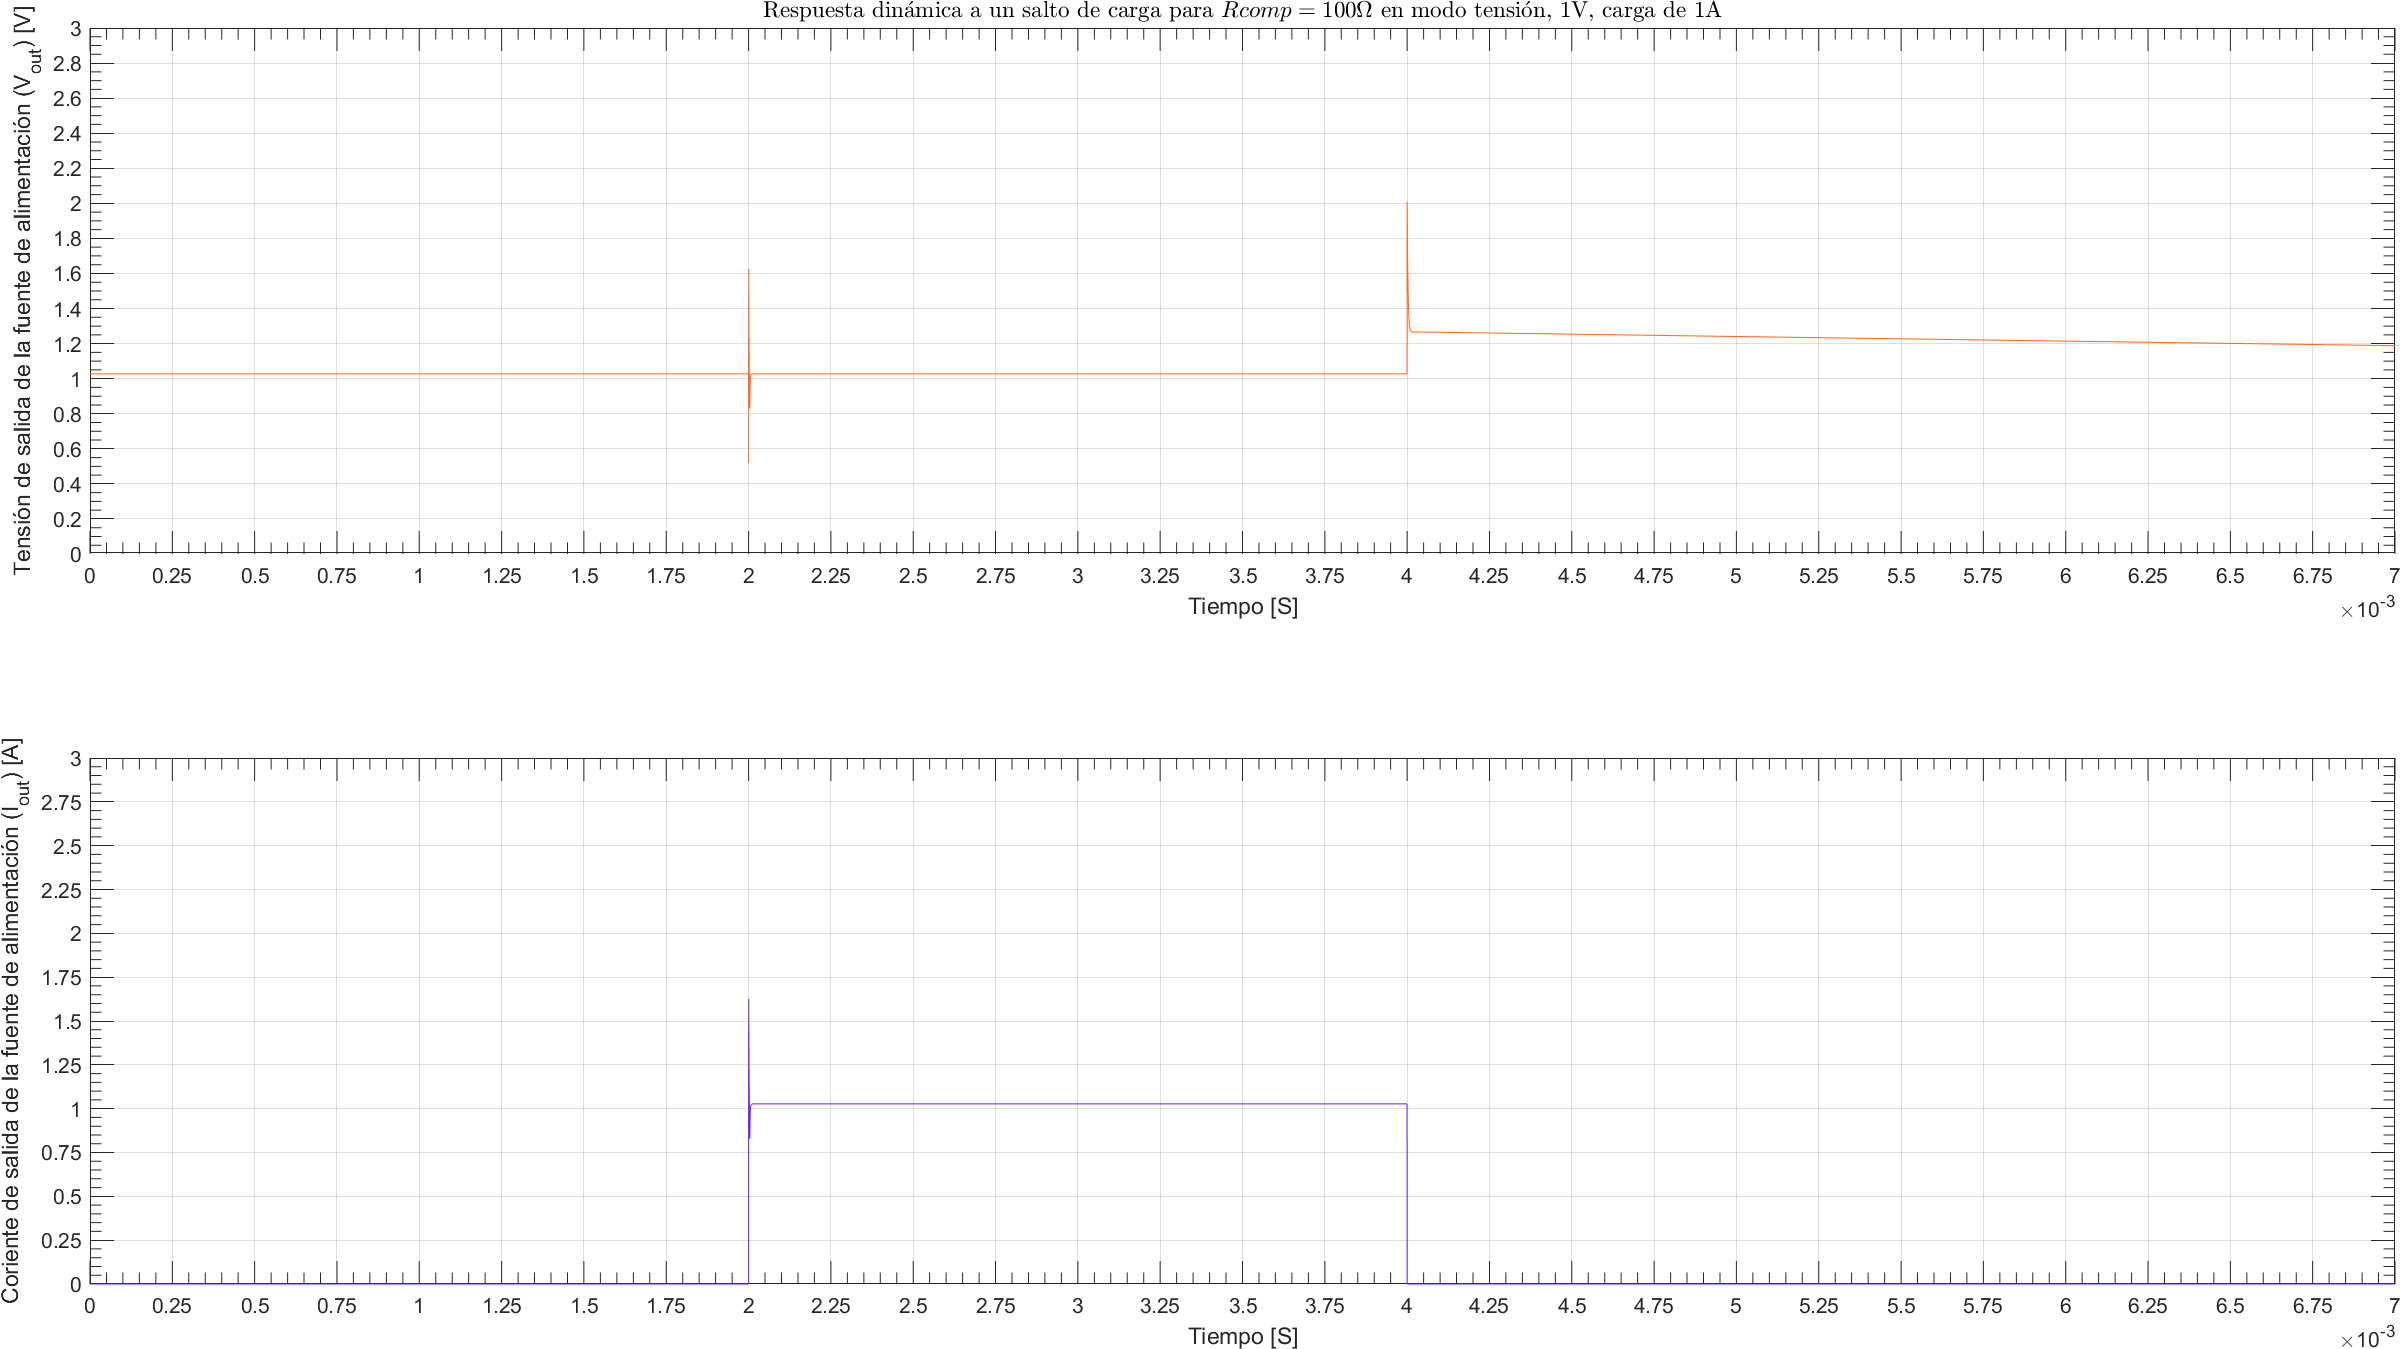
\includegraphics[width=1.1 \textwidth, angle=90]{./img/plots/dynamic/power_supply_RCOMP_100_STEP_Modo2.png}
\caption{\label{fig:fig_power_supply_RCOMP_STEP_20n_Modo2}\footnotesize{Respuesta dinámica en modo tensión, $V_{out} = 1 \si[per-mode=symbol]{\volt}$, para $R_{comp} = 100 \si[per-mode=symbol]{\ohm} $.}}
\end{center}
\end{figure}

\clearpage


\subsubsection{Análisis para $R_{comp}$ en modo corriente, $I_{out} = 2 \si[per-mode=symbol]{\ampere}$, $R_{L} = 0 \si[per-mode=symbol]{\ohm}$}
% RCOMP MODO 3.

\clearpage

\begin{figure}[H] %htb
\begin{center}
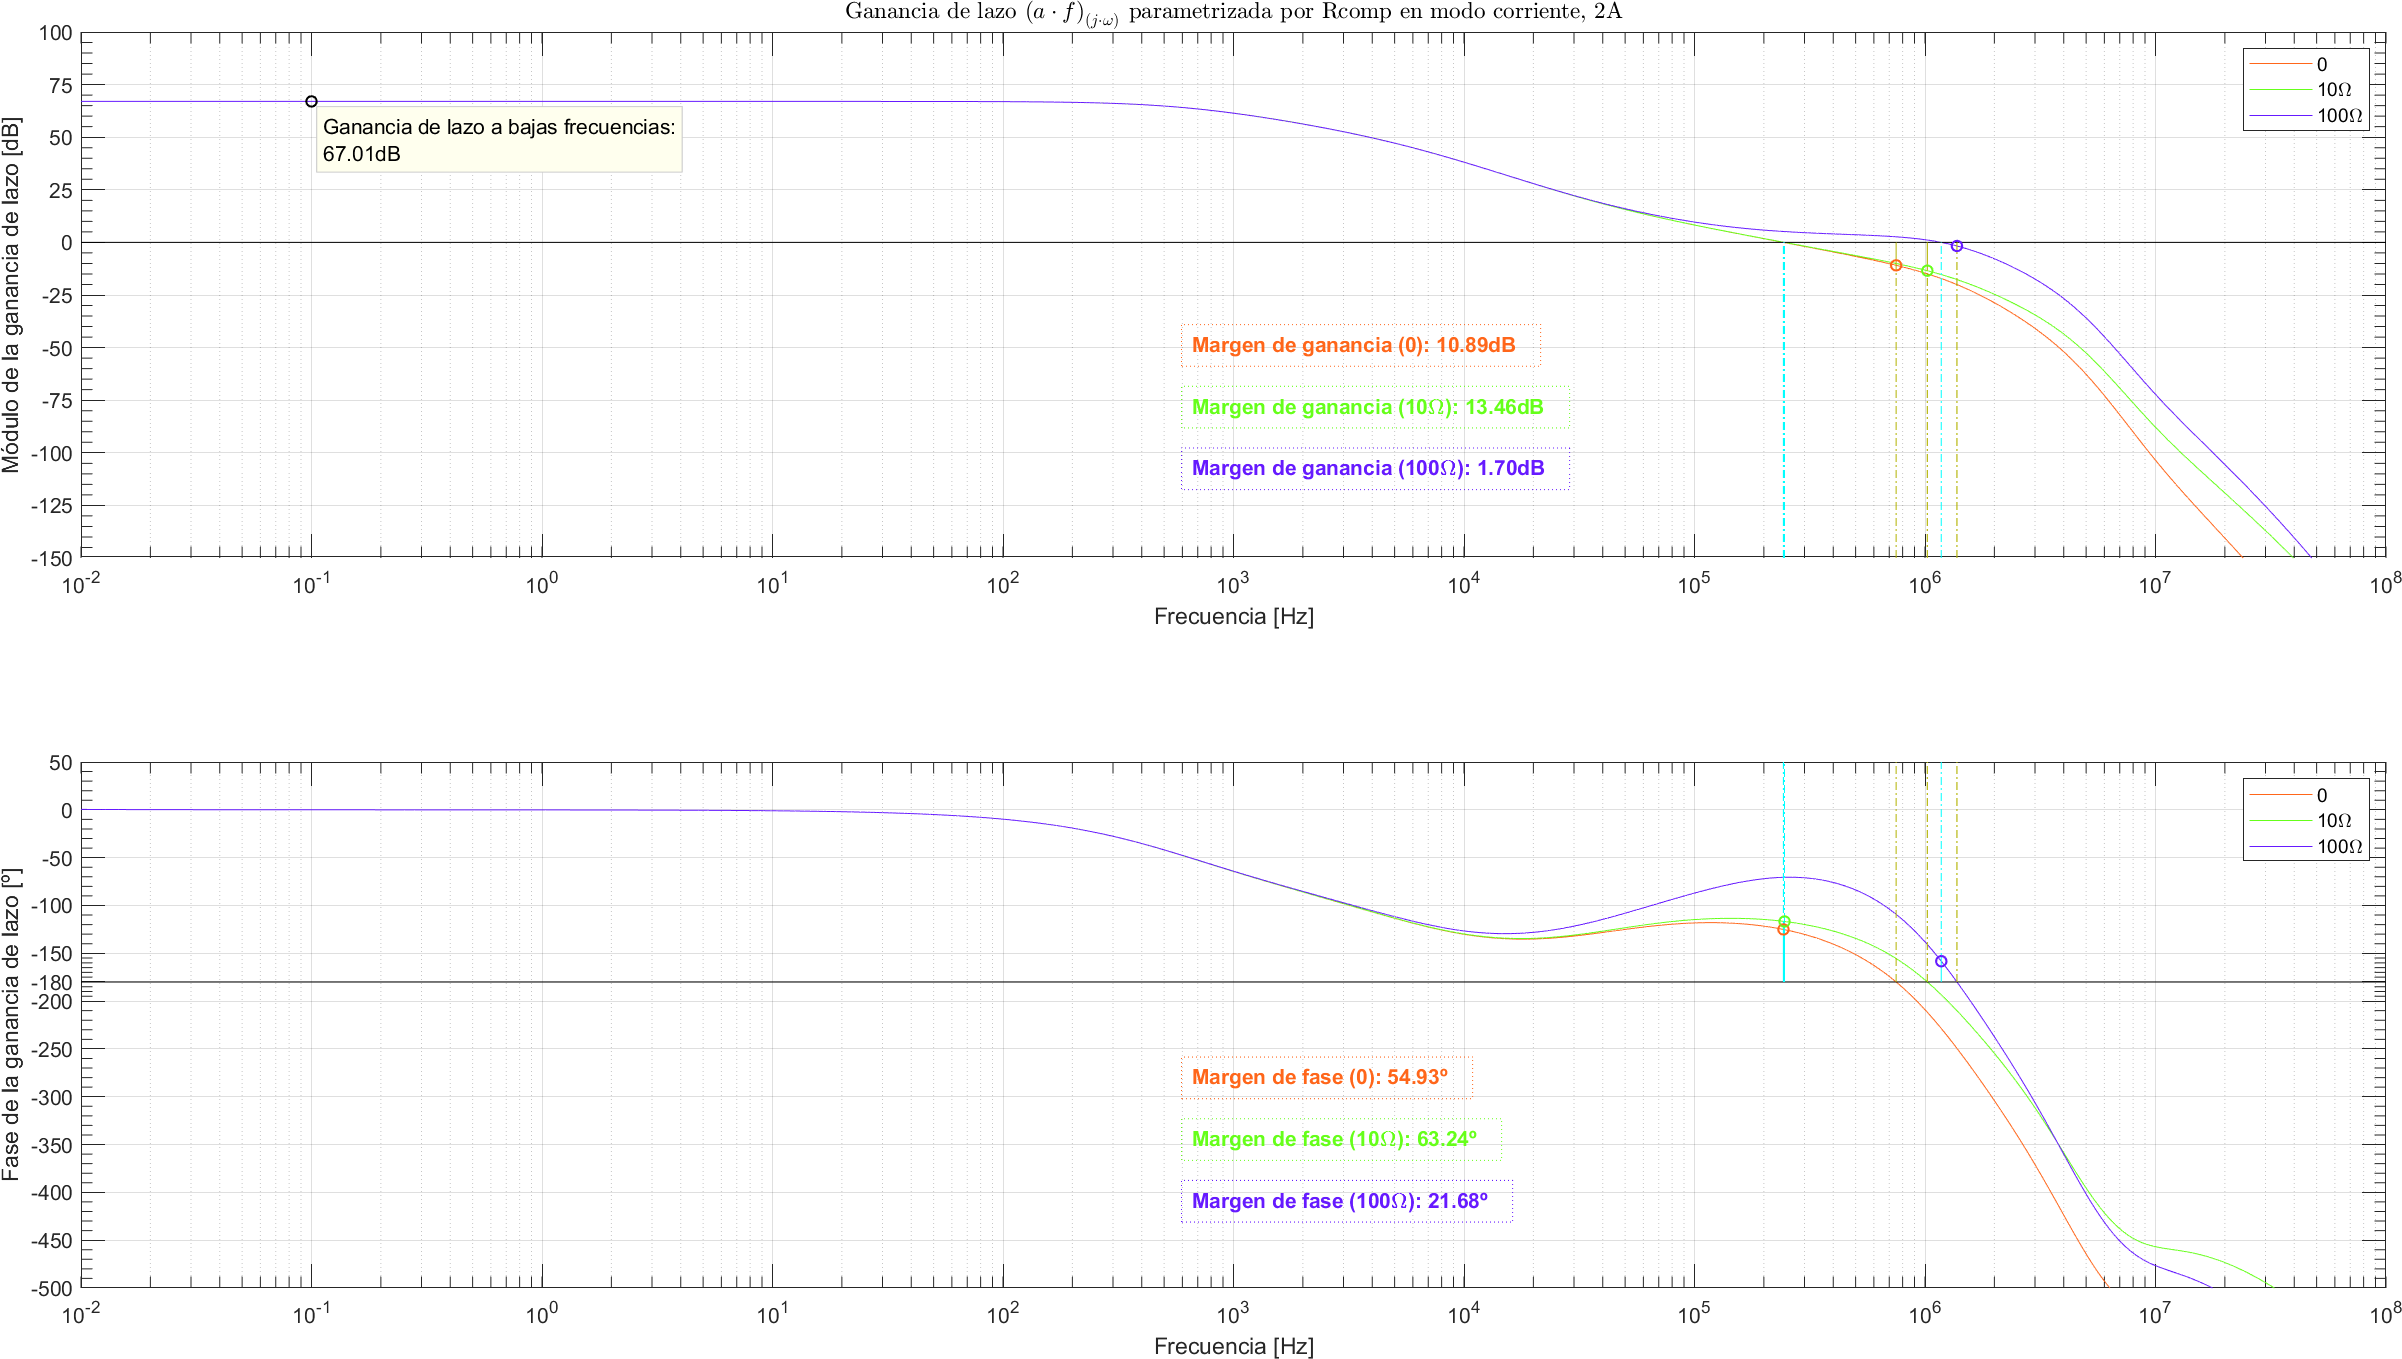
\includegraphics[width=1.1 \textwidth, angle=90]{./img/plots/loop/power_supply_RCOMP_LOOP_Modo3.png}
\caption{\label{fig:fig_power_supply_RCOMP_LOOP_Modo3}\footnotesize{Ganancia de lazo en modo corriente, $I_{out} = 2 \si[per-mode=symbol]{\ampere}$, en función de la frecuencia parametrizada por $R_{comp}$.}}
\end{center}
\end{figure}


\clearpage

\begin{figure}[H] %htb
\begin{center}
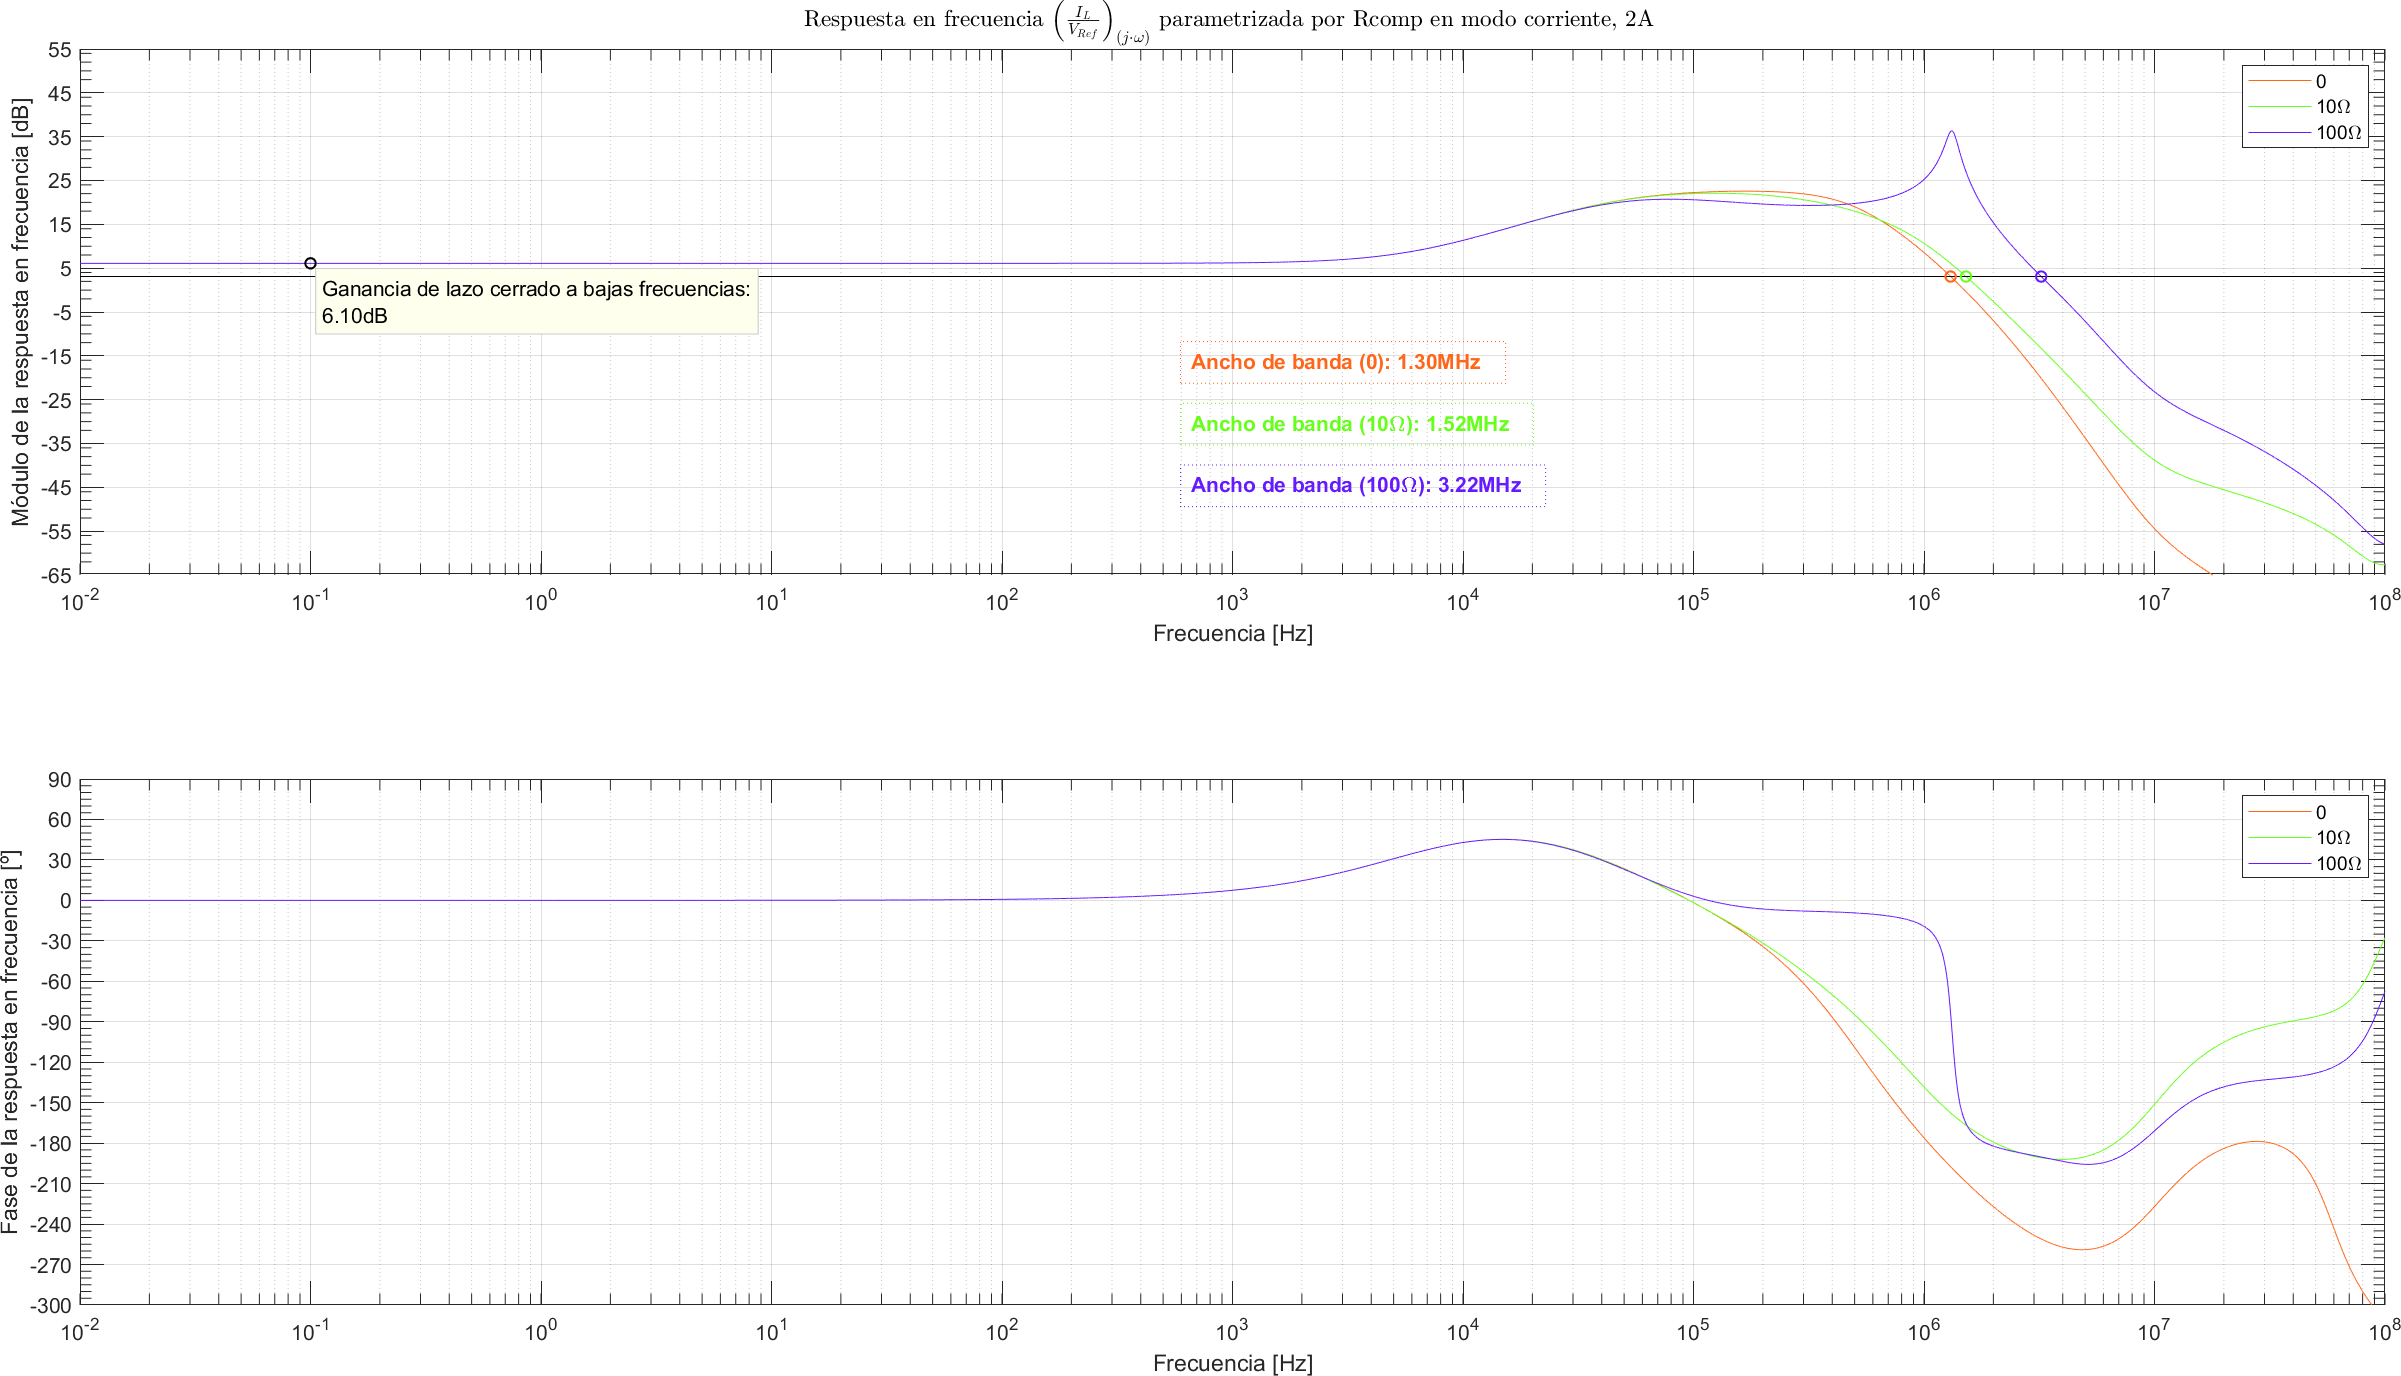
\includegraphics[width=1.1 \textwidth, angle=90]{./img/plots/rf/power_supply_RCOMP_RF_Modo3.png}
\caption{\label{fig:fig_power_supply_RCOMP_RF_Modo3}\footnotesize{Respuesta en frecuencia en modo corriente, $I_{out} = 2 \si[per-mode=symbol]{\ampere}$, en función de la frecuencia parametrizada por $R_{comp}$.}}
\end{center}
\end{figure}

\clearpage

\begin{figure}[H] %htb
\begin{center}
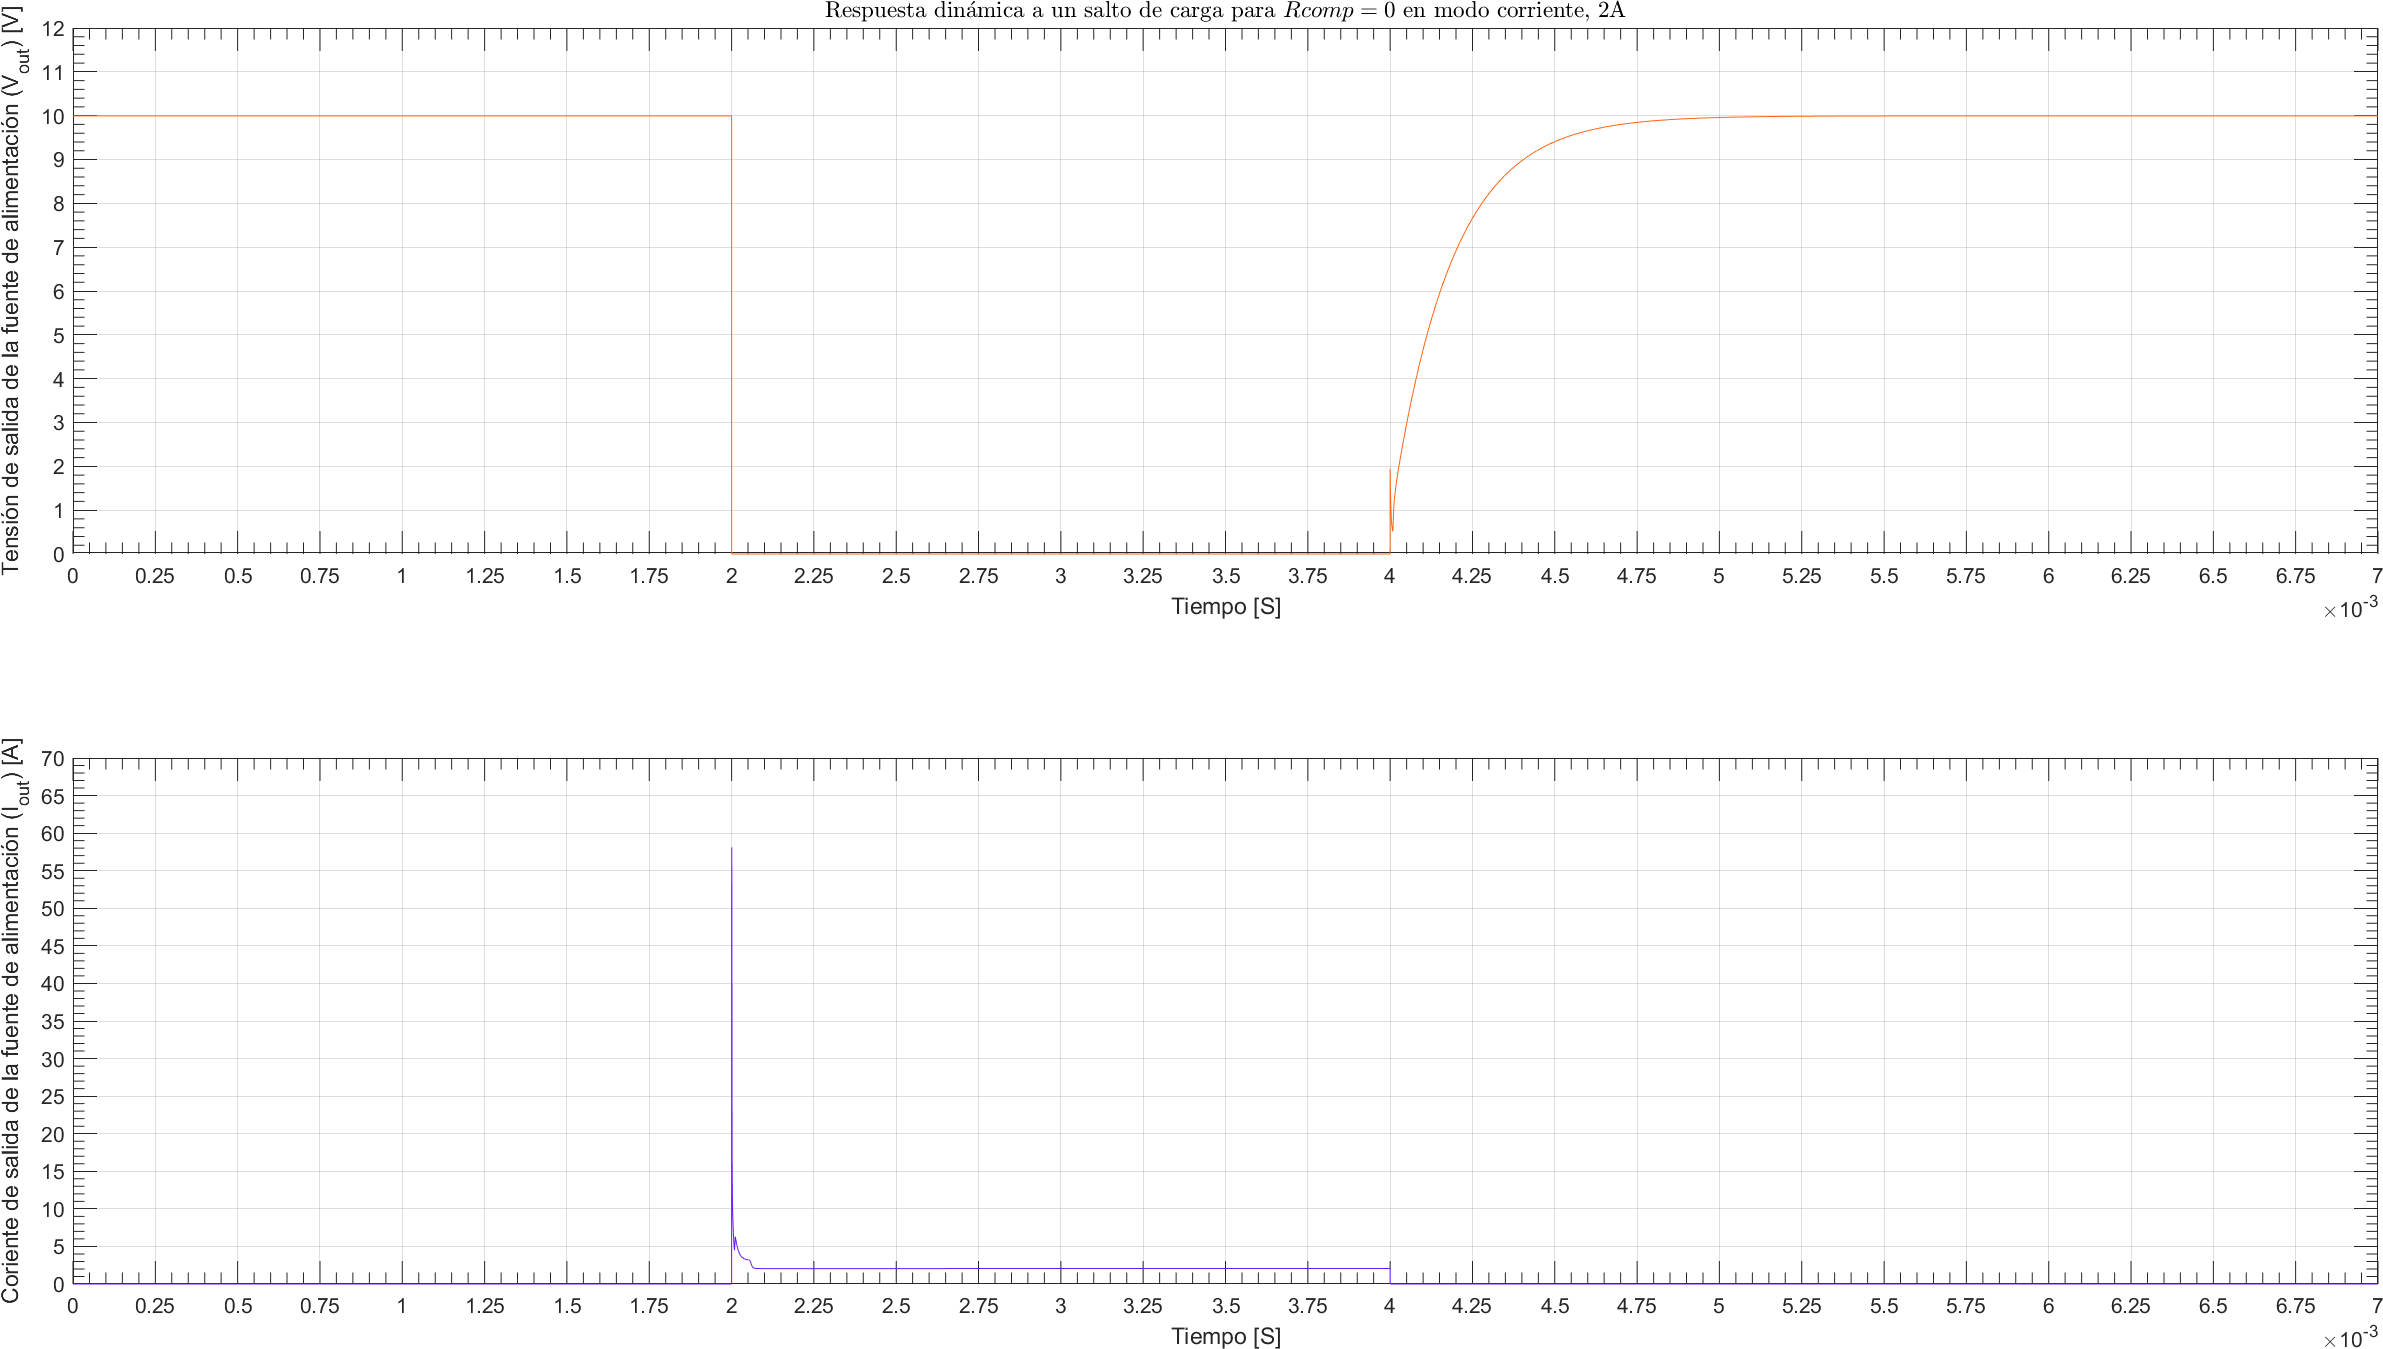
\includegraphics[width=1.1 \textwidth, angle=90]{./img/plots/dynamic/power_supply_RCOMP_0_STEP_Modo3.png}
\caption{\label{fig:fig_power_supply_RCOMP_STEP_0_Modo3}\footnotesize{Respuesta dinámica en modo corriente, $I_{out} = 2 \si[per-mode=symbol]{\ampere}$, para $R_{comp} = 0 \si[per-mode=symbol]{\ohm} $.}}
\end{center}
\end{figure}

\clearpage

\begin{figure}[H] %htb
\begin{center}
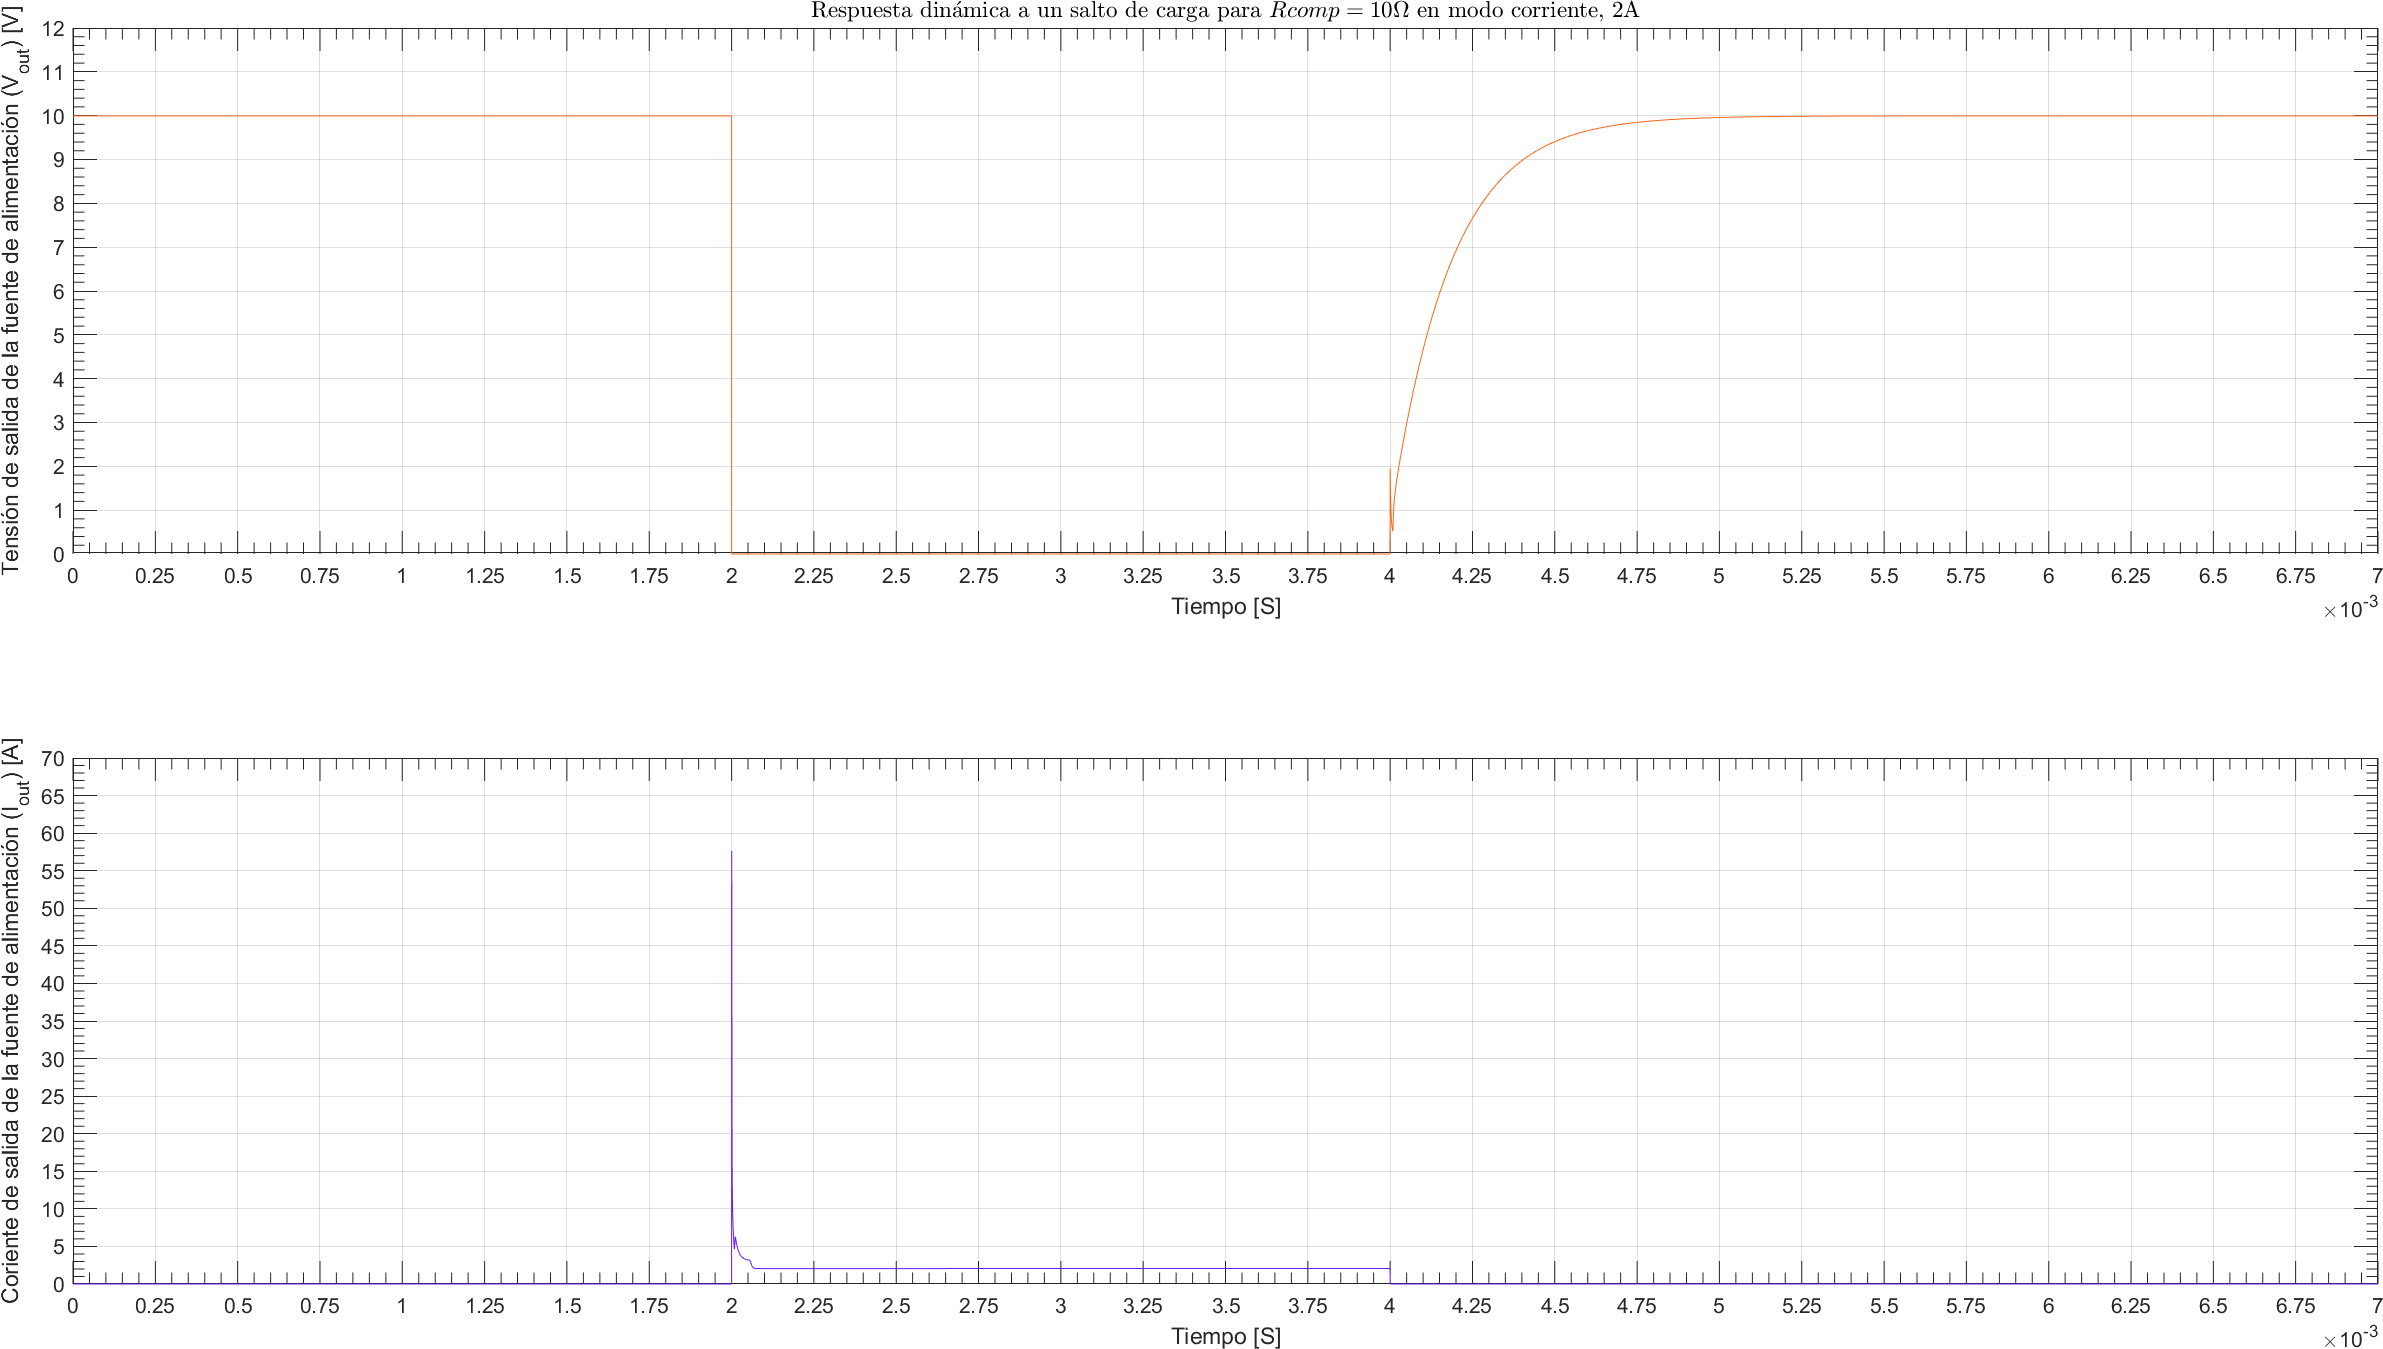
\includegraphics[width=1.1 \textwidth, angle=90]{./img/plots/dynamic/power_supply_RCOMP_10_STEP_Modo3.png}
\caption{\label{fig:fig_power_supply_RCOMP_STEP_10_Modo3}\footnotesize{Respuesta dinámica en modo corriente, $I_{out} = 2 \si[per-mode=symbol]{\ampere}$, para $R_{comp} = 10 \si[per-mode=symbol]{\ohm} $.}}
\end{center}
\end{figure}

\clearpage

\begin{figure}[H] %htb
\begin{center}
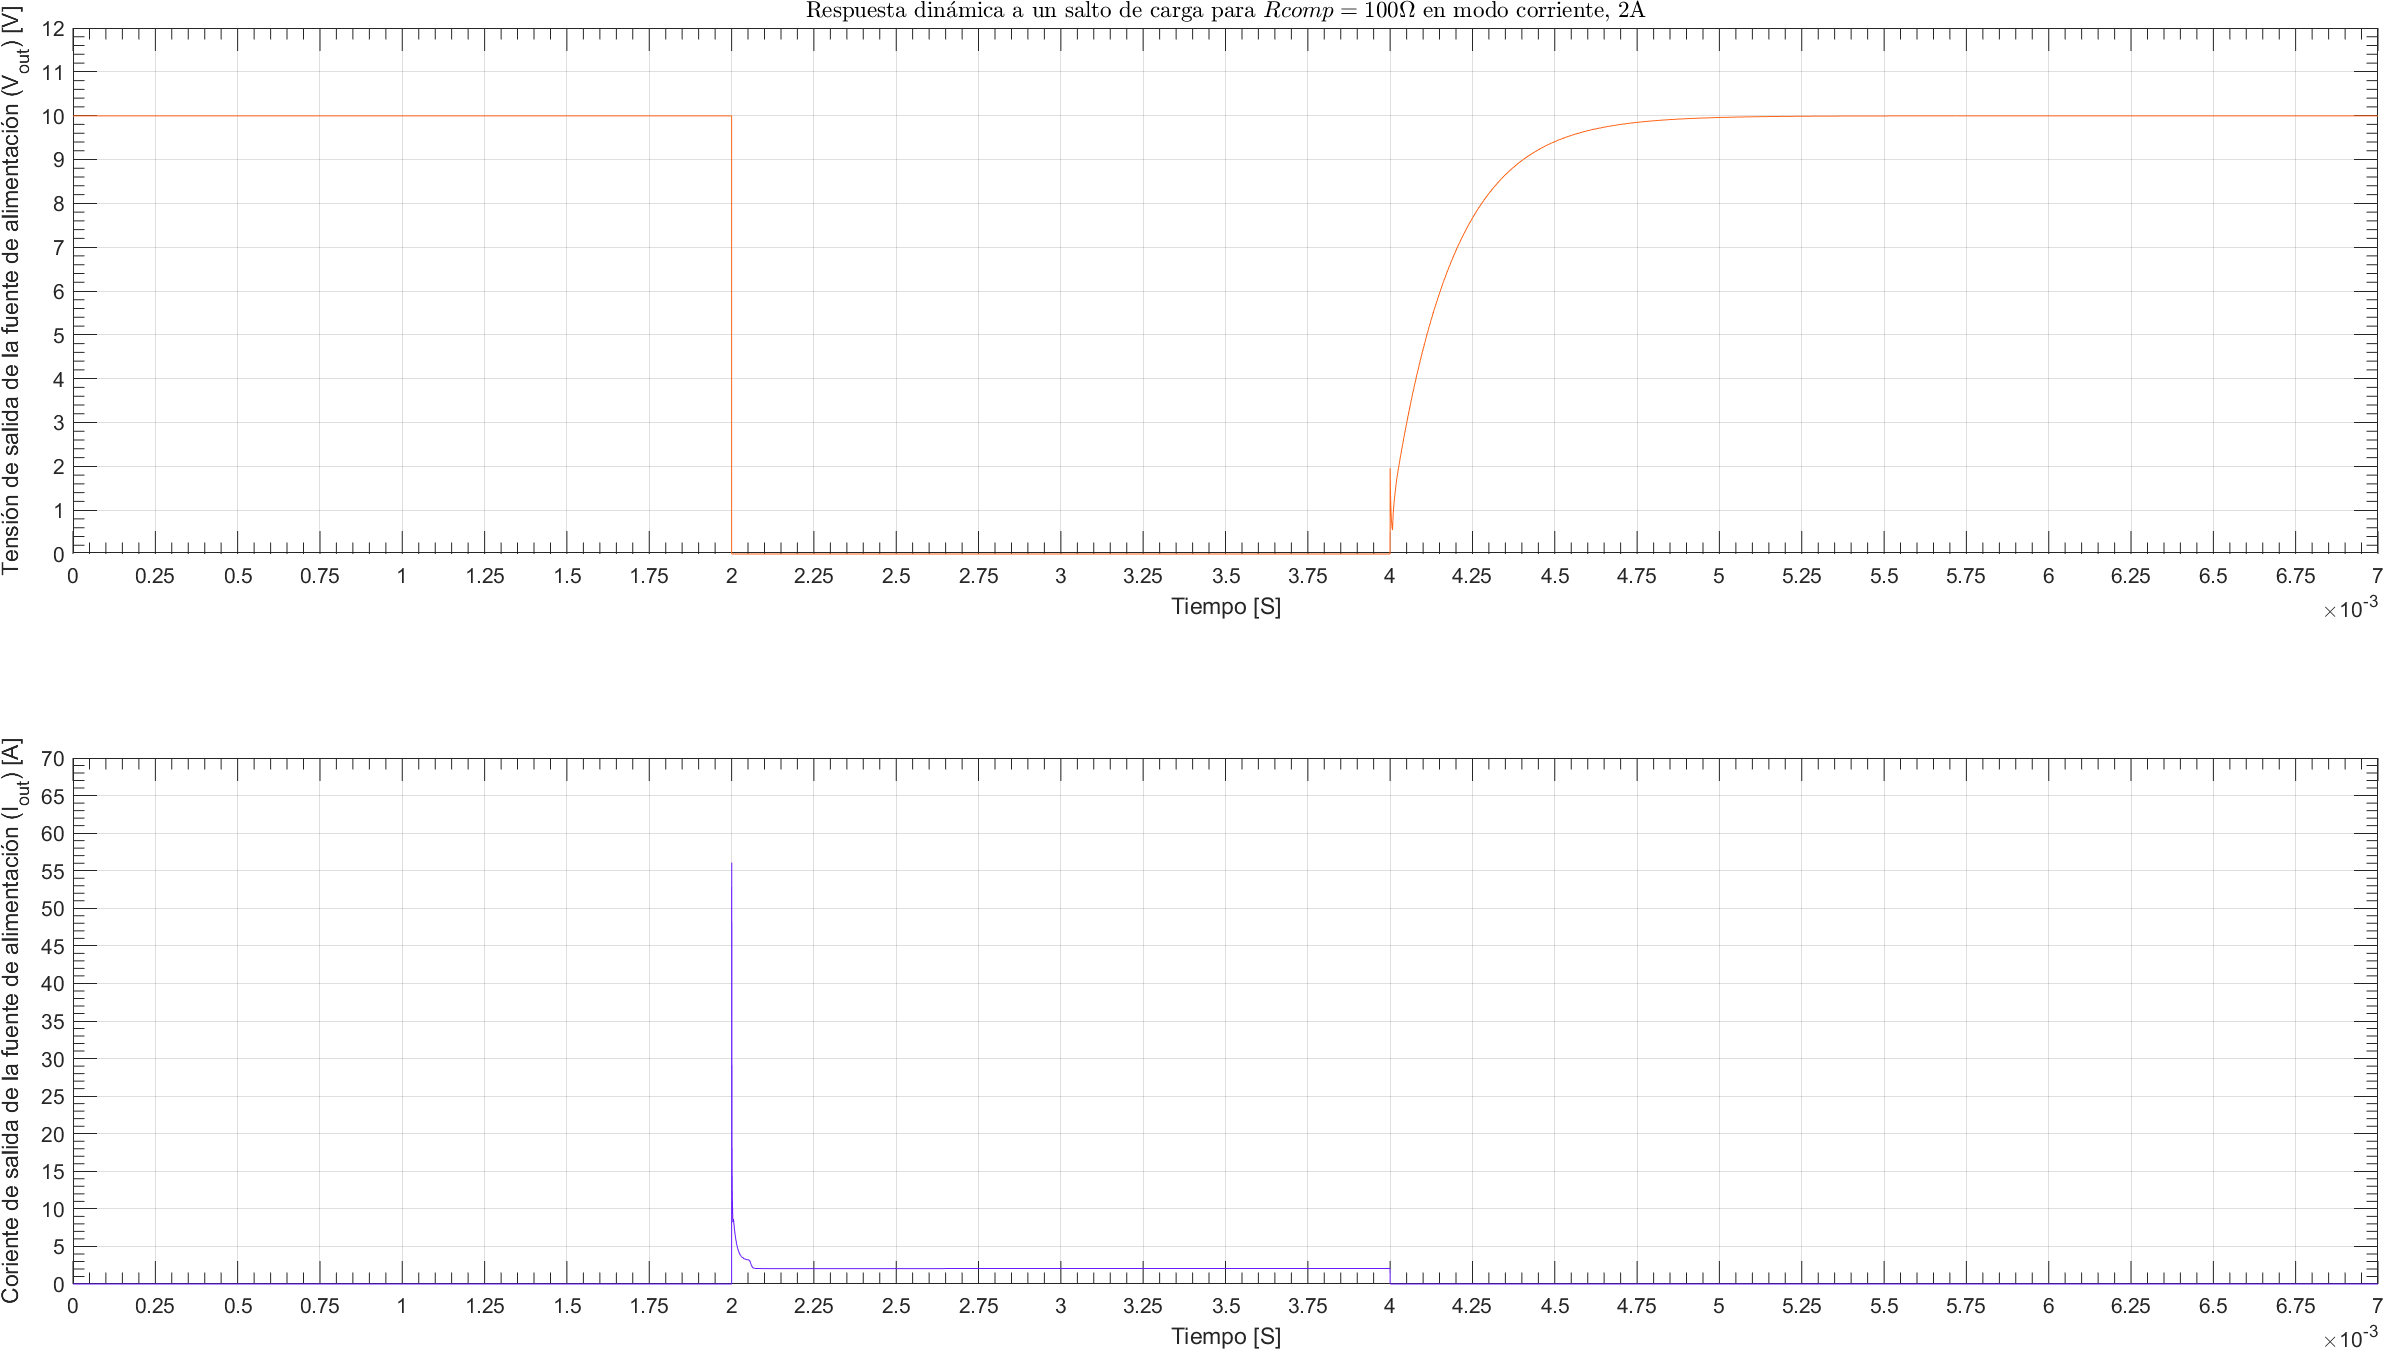
\includegraphics[width=1.1 \textwidth, angle=90]{./img/plots/dynamic/power_supply_RCOMP_100_STEP_Modo3.png}
\caption{\label{fig:fig_power_supply_RCOMP_STEP_100_Modo3}\footnotesize{Respuesta dinámica en modo corriente, $I_{out} = 2 \si[per-mode=symbol]{\ampere}$, para $R_{comp} = 100 \si[per-mode=symbol]{\ohm} $.}}
\end{center}
\end{figure}

\clearpage


\subsubsection{Análisis para $R_{comp}$ en modo corriente, $I_{out} = 200 \si[per-mode=symbol]{\milli\ampere}$, $R_{L} = 0 \si[per-mode=symbol]{\ohm}$}
% RCOMP MODO 4.

\clearpage

\begin{figure}[H] %htb
\begin{center}
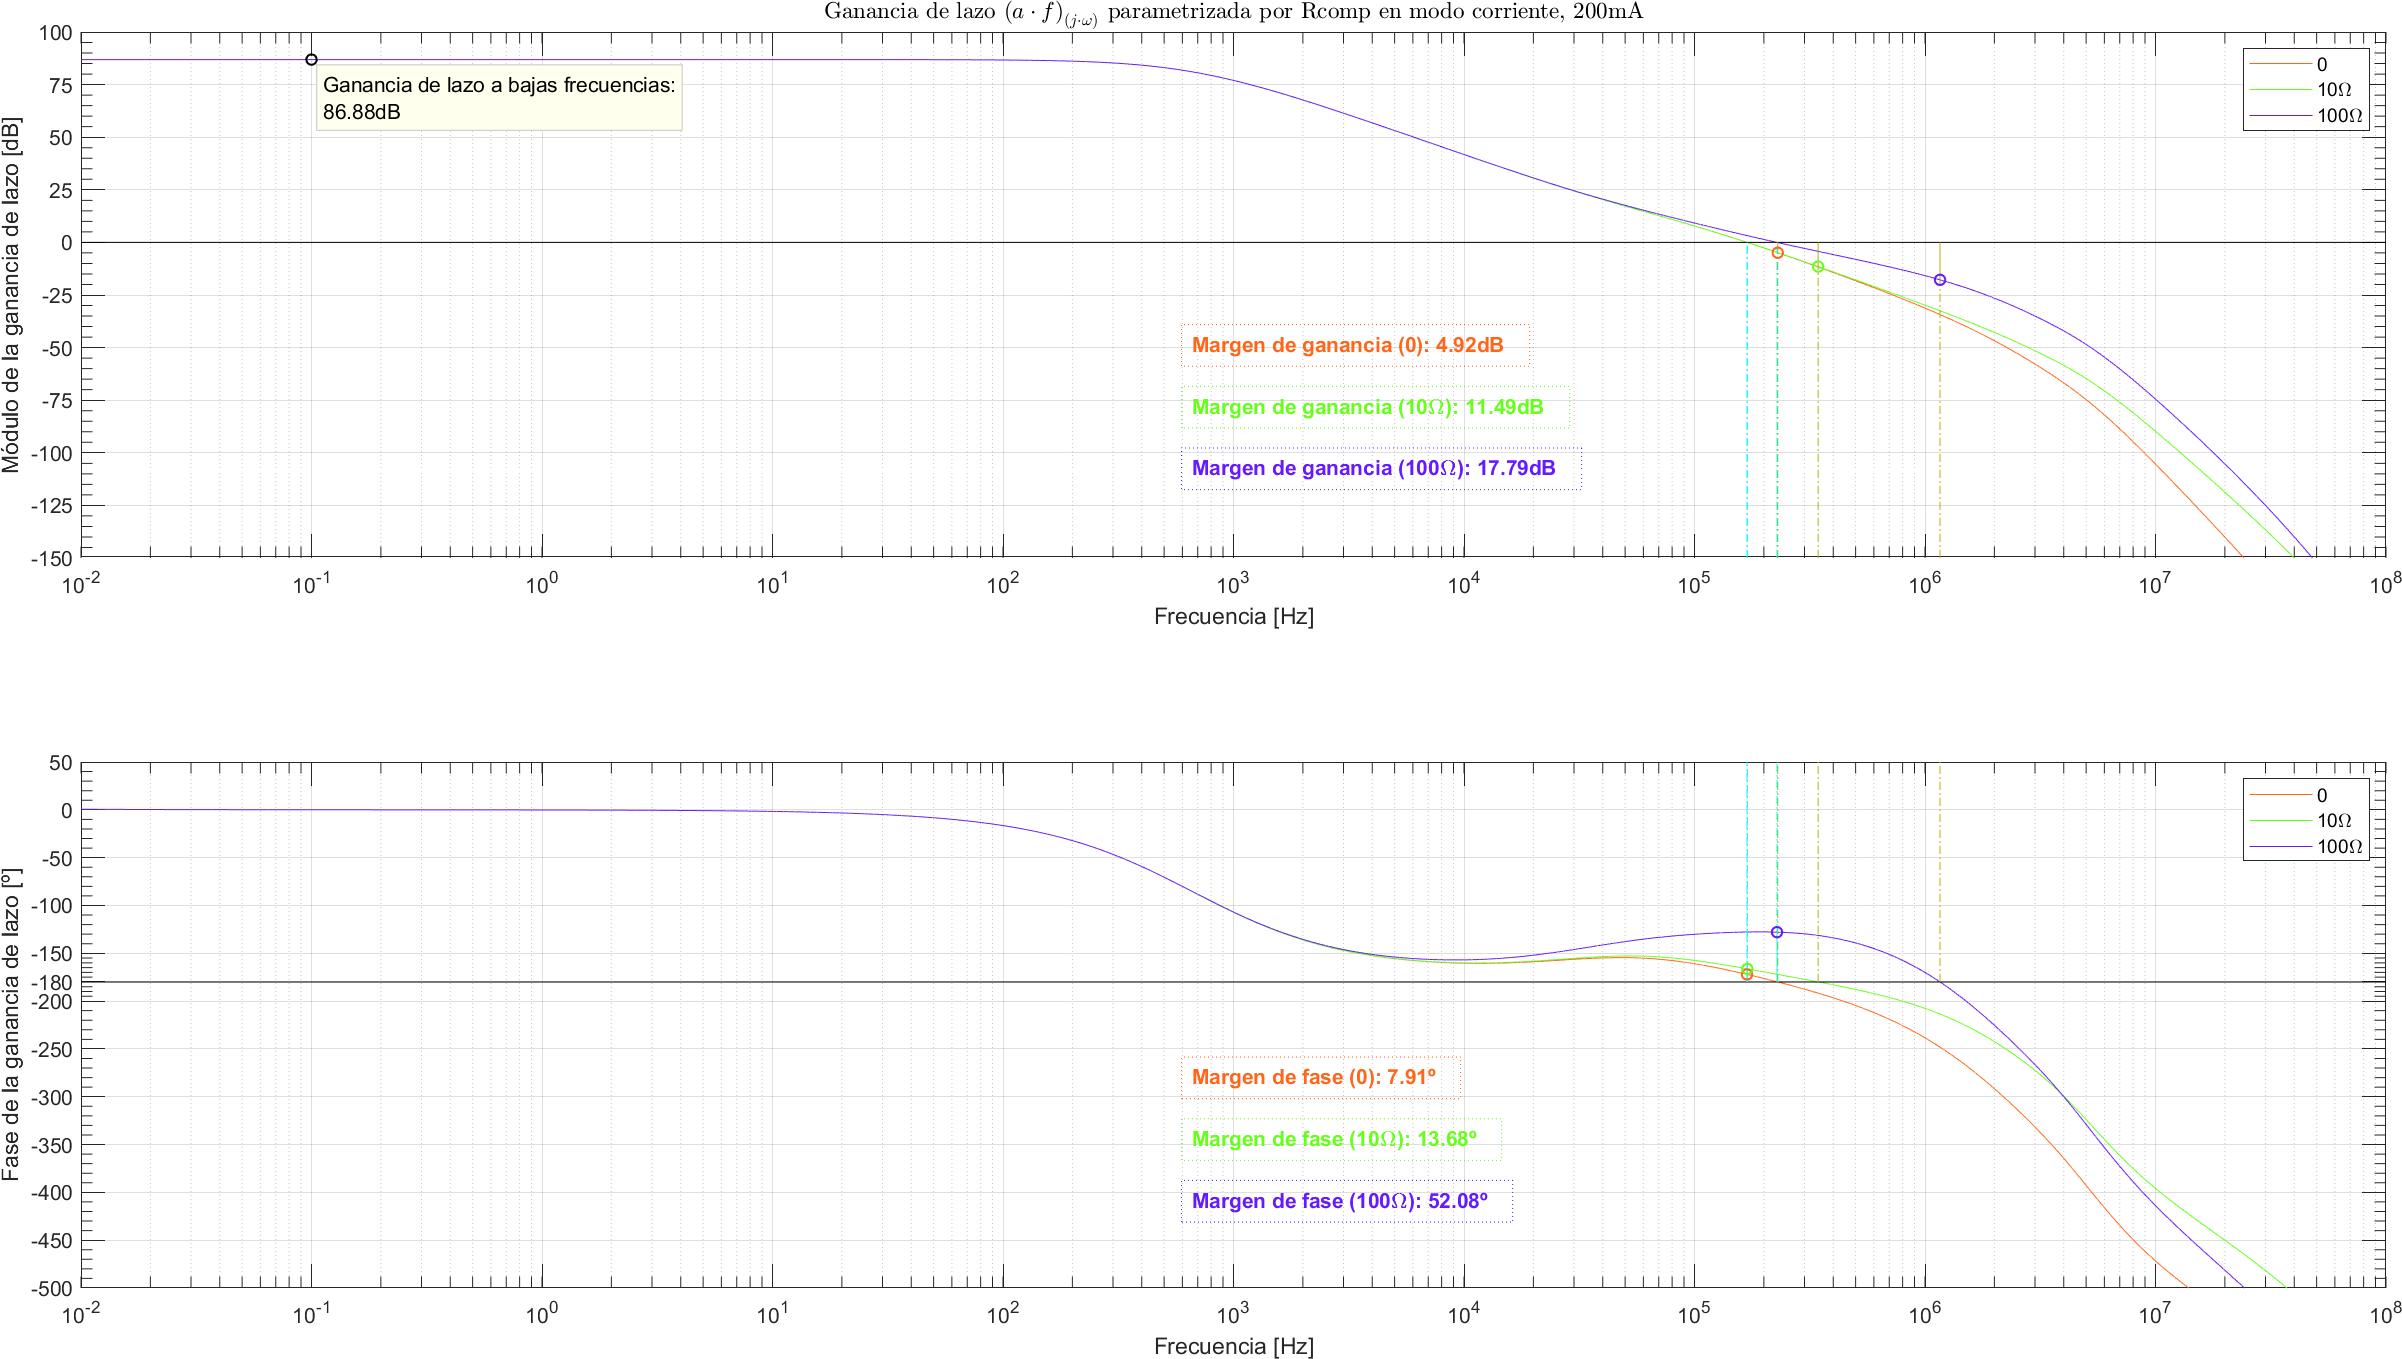
\includegraphics[width=1.1 \textwidth, angle=90]{./img/plots/loop/power_supply_RCOMP_LOOP_Modo4.png}
\caption{\label{fig:fig_power_supply_RCOMP_LOOP_Modo4}\footnotesize{Ganancia de lazo en modo corriente, $I_{out} = 200 \si[per-mode=symbol]{\milli\ampere}$, en función de la frecuencia parametrizada por $R_{comp}$.}}
\end{center}
\end{figure}


\clearpage

\begin{figure}[H] %htb
\begin{center}
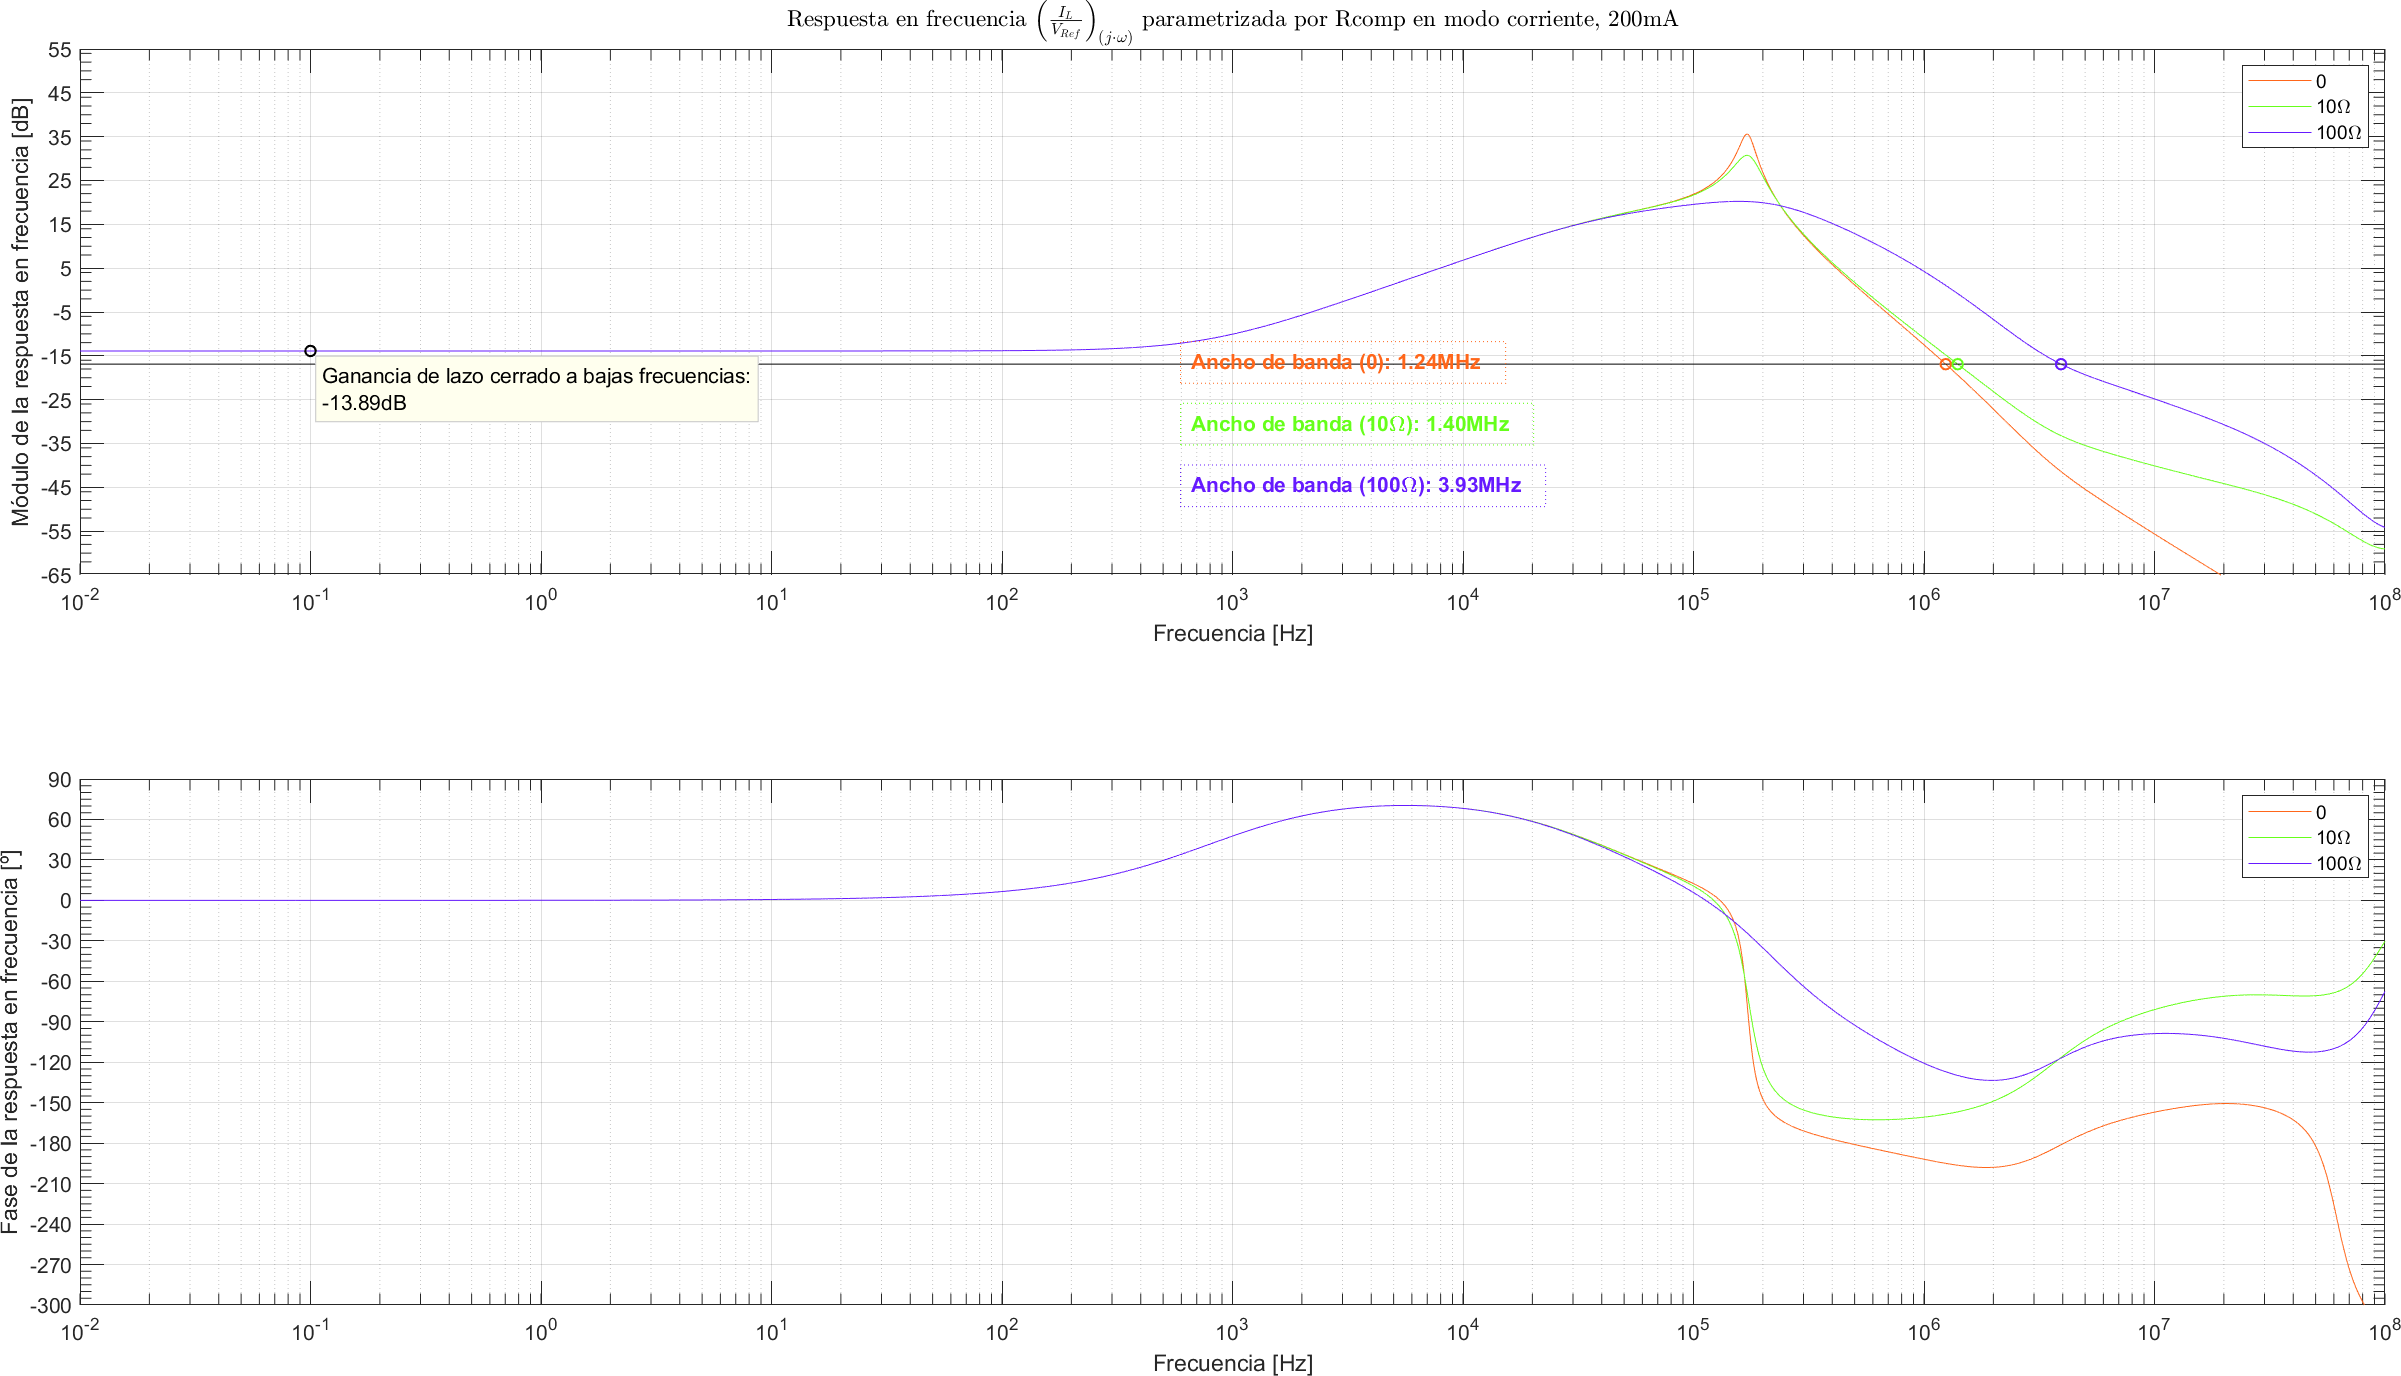
\includegraphics[width=1.1 \textwidth, angle=90]{./img/plots/rf/power_supply_RCOMP_RF_Modo4.png}
\caption{\label{fig:fig_power_supply_RCOMP_RF_Modo4}\footnotesize{Respuesta en frecuencia en modo corriente, $I_{out} = 200 \si[per-mode=symbol]{\milli\ampere}$, en función de la frecuencia parametrizada por $R_{comp}$.}}
\end{center}
\end{figure}

\clearpage

\begin{figure}[H] %htb
\begin{center}
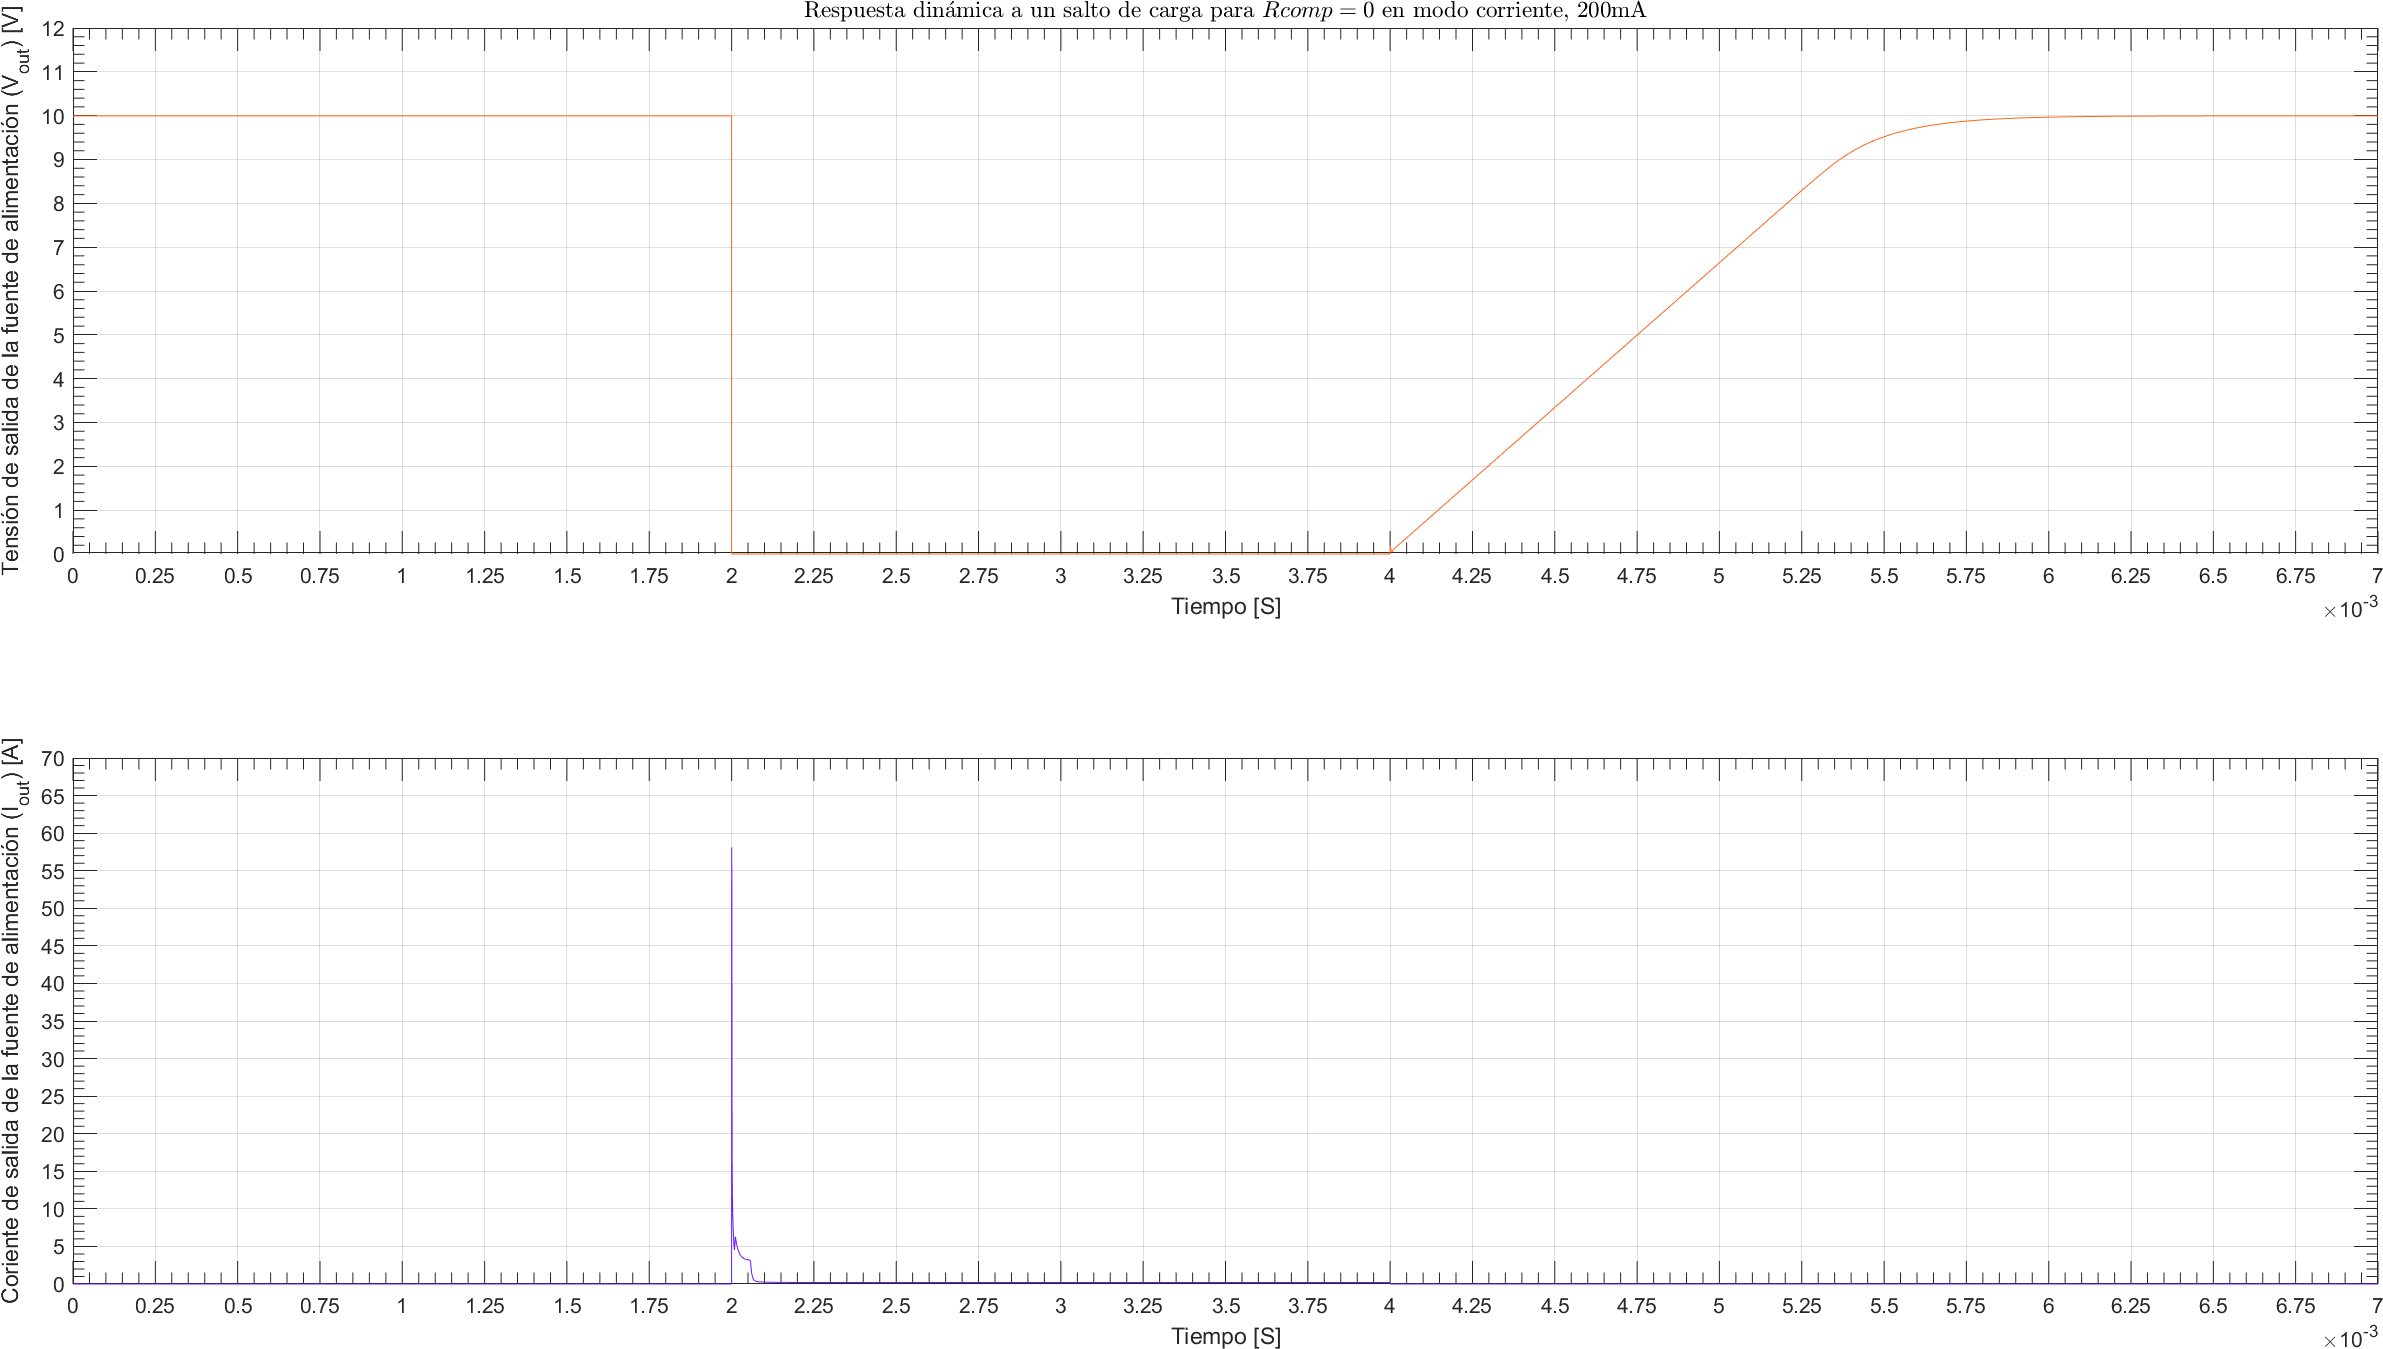
\includegraphics[width=1.1 \textwidth, angle=90]{./img/plots/dynamic/power_supply_RCOMP_0_STEP_Modo4.png}
\caption{\label{fig:fig_power_supply_RCOMP_STEP_0_Modo4}\footnotesize{Respuesta dinámica en modo corriente, $I_{out} = 200 \si[per-mode=symbol]{\milli\ampere}$, para $R_{comp} = 0 \si[per-mode=symbol]{\ohm} $.}}
\end{center}
\end{figure}

\clearpage

\begin{figure}[H] %htb
\begin{center}
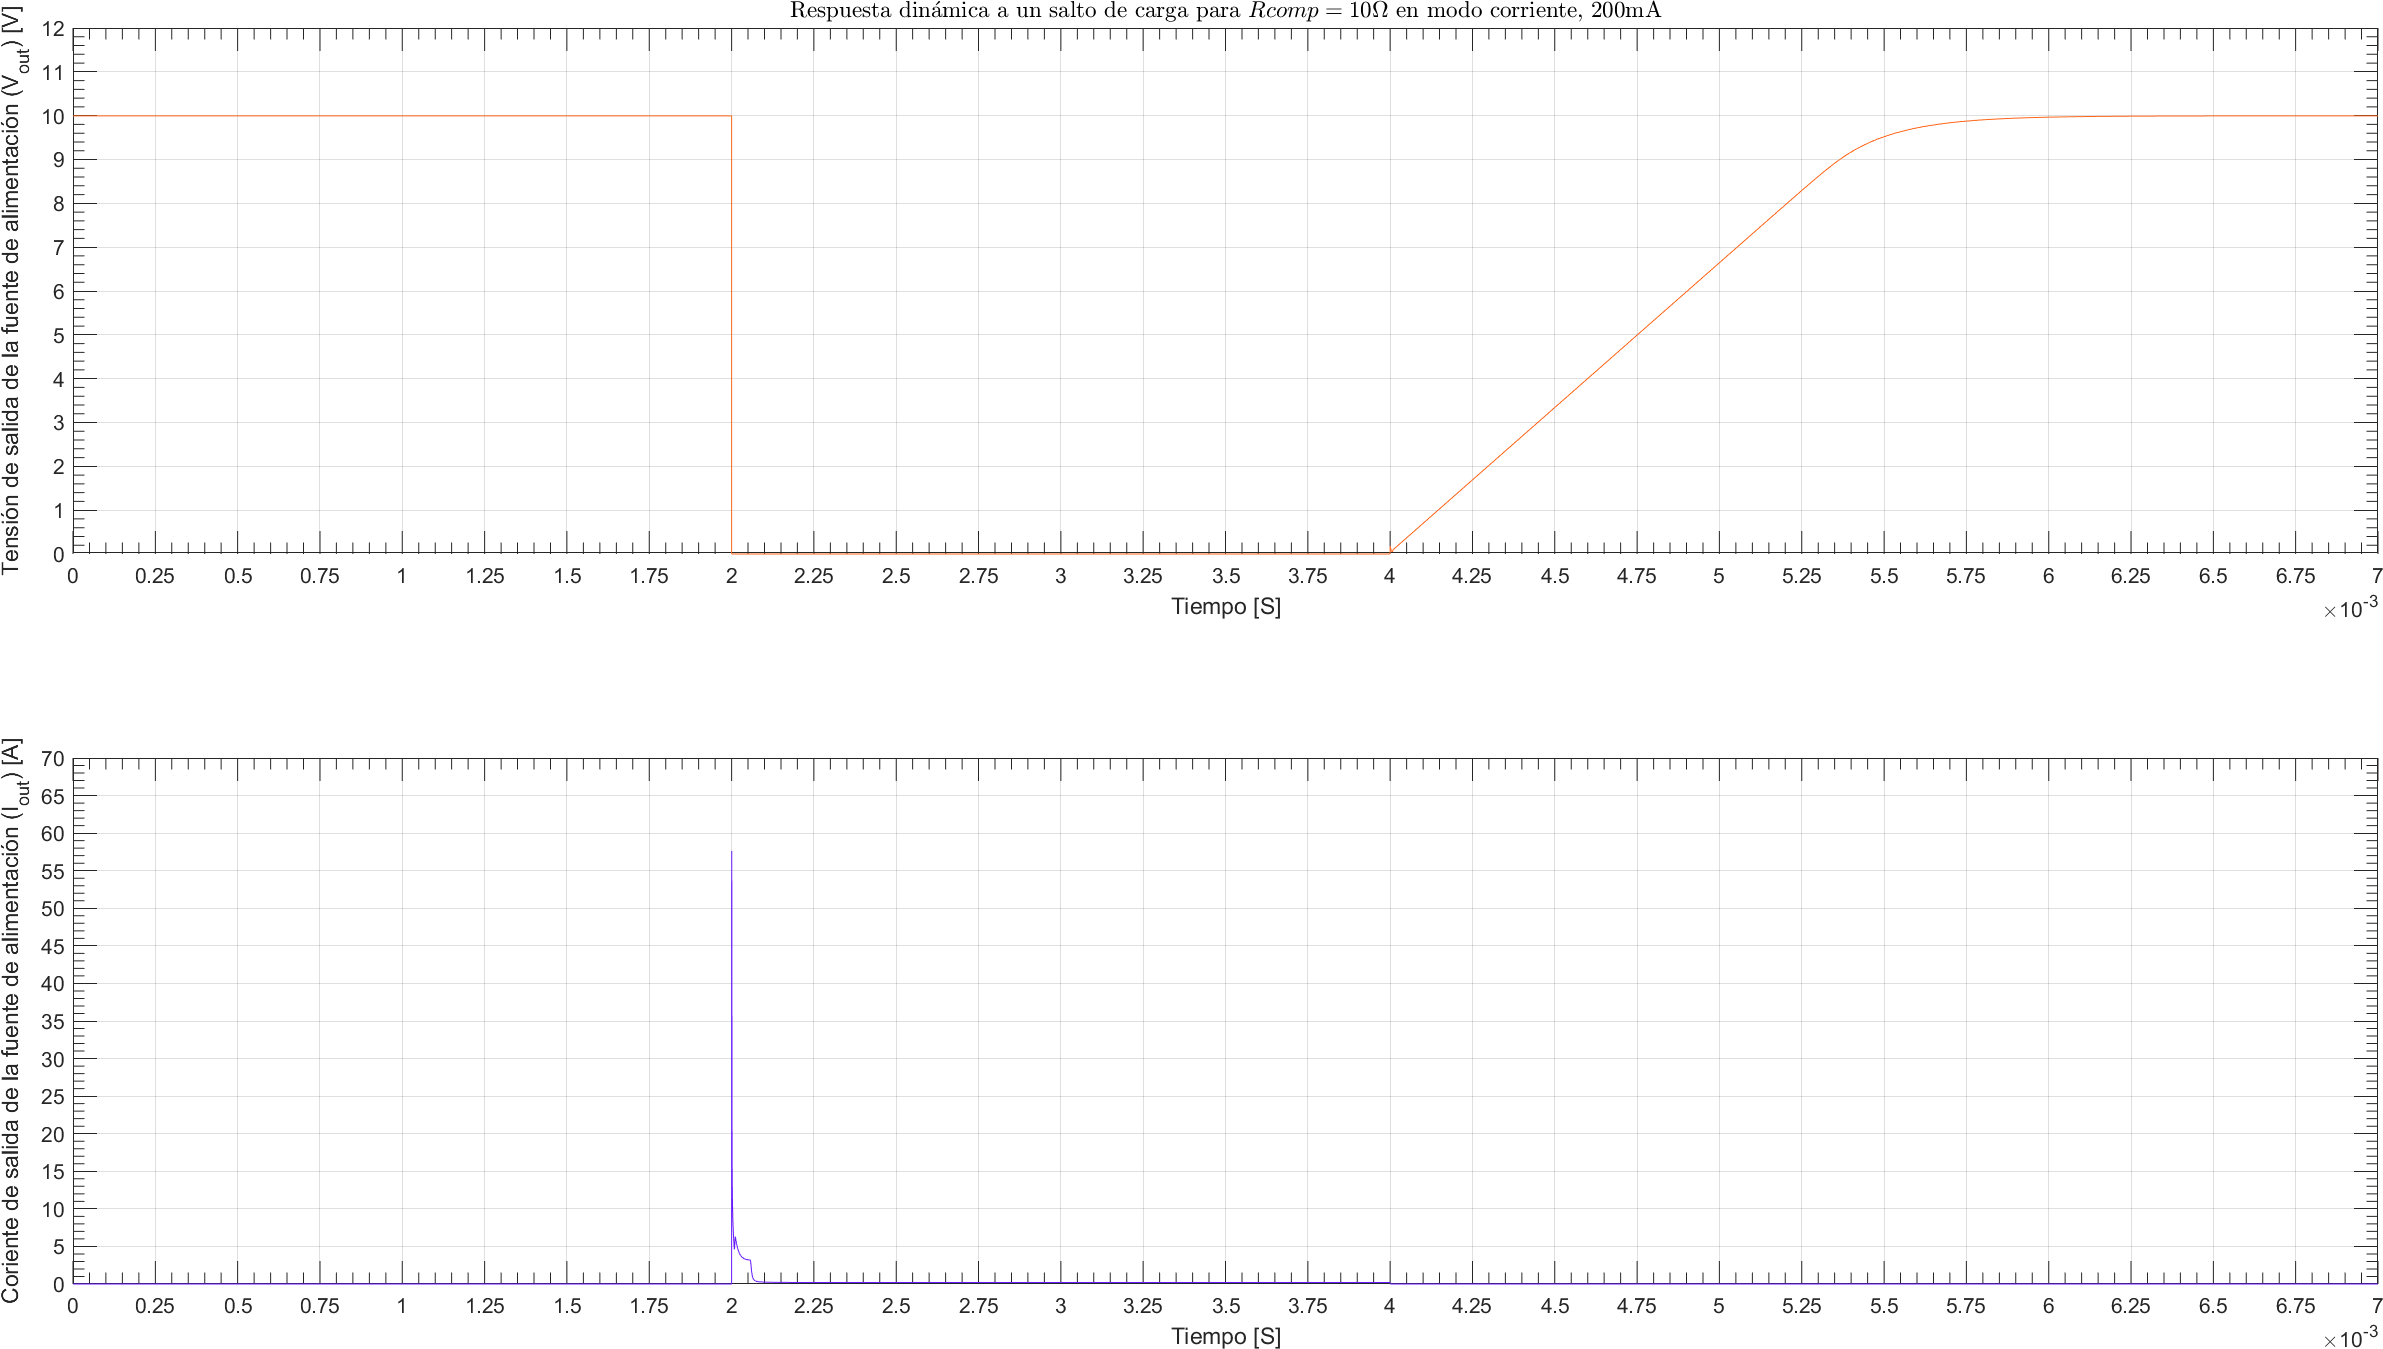
\includegraphics[width=1.1 \textwidth, angle=90]{./img/plots/dynamic/power_supply_RCOMP_10_STEP_Modo4.png}
\caption{\label{fig:fig_power_supply_RCOMP_STEP_10_Modo4}\footnotesize{Respuesta dinámica en modo corriente, $I_{out} = 200 \si[per-mode=symbol]{\milli\ampere}$, para $R_{comp} = 10 \si[per-mode=symbol]{\ohm} $.}}
\end{center}
\end{figure}

\clearpage

\begin{figure}[H] %htb
\begin{center}
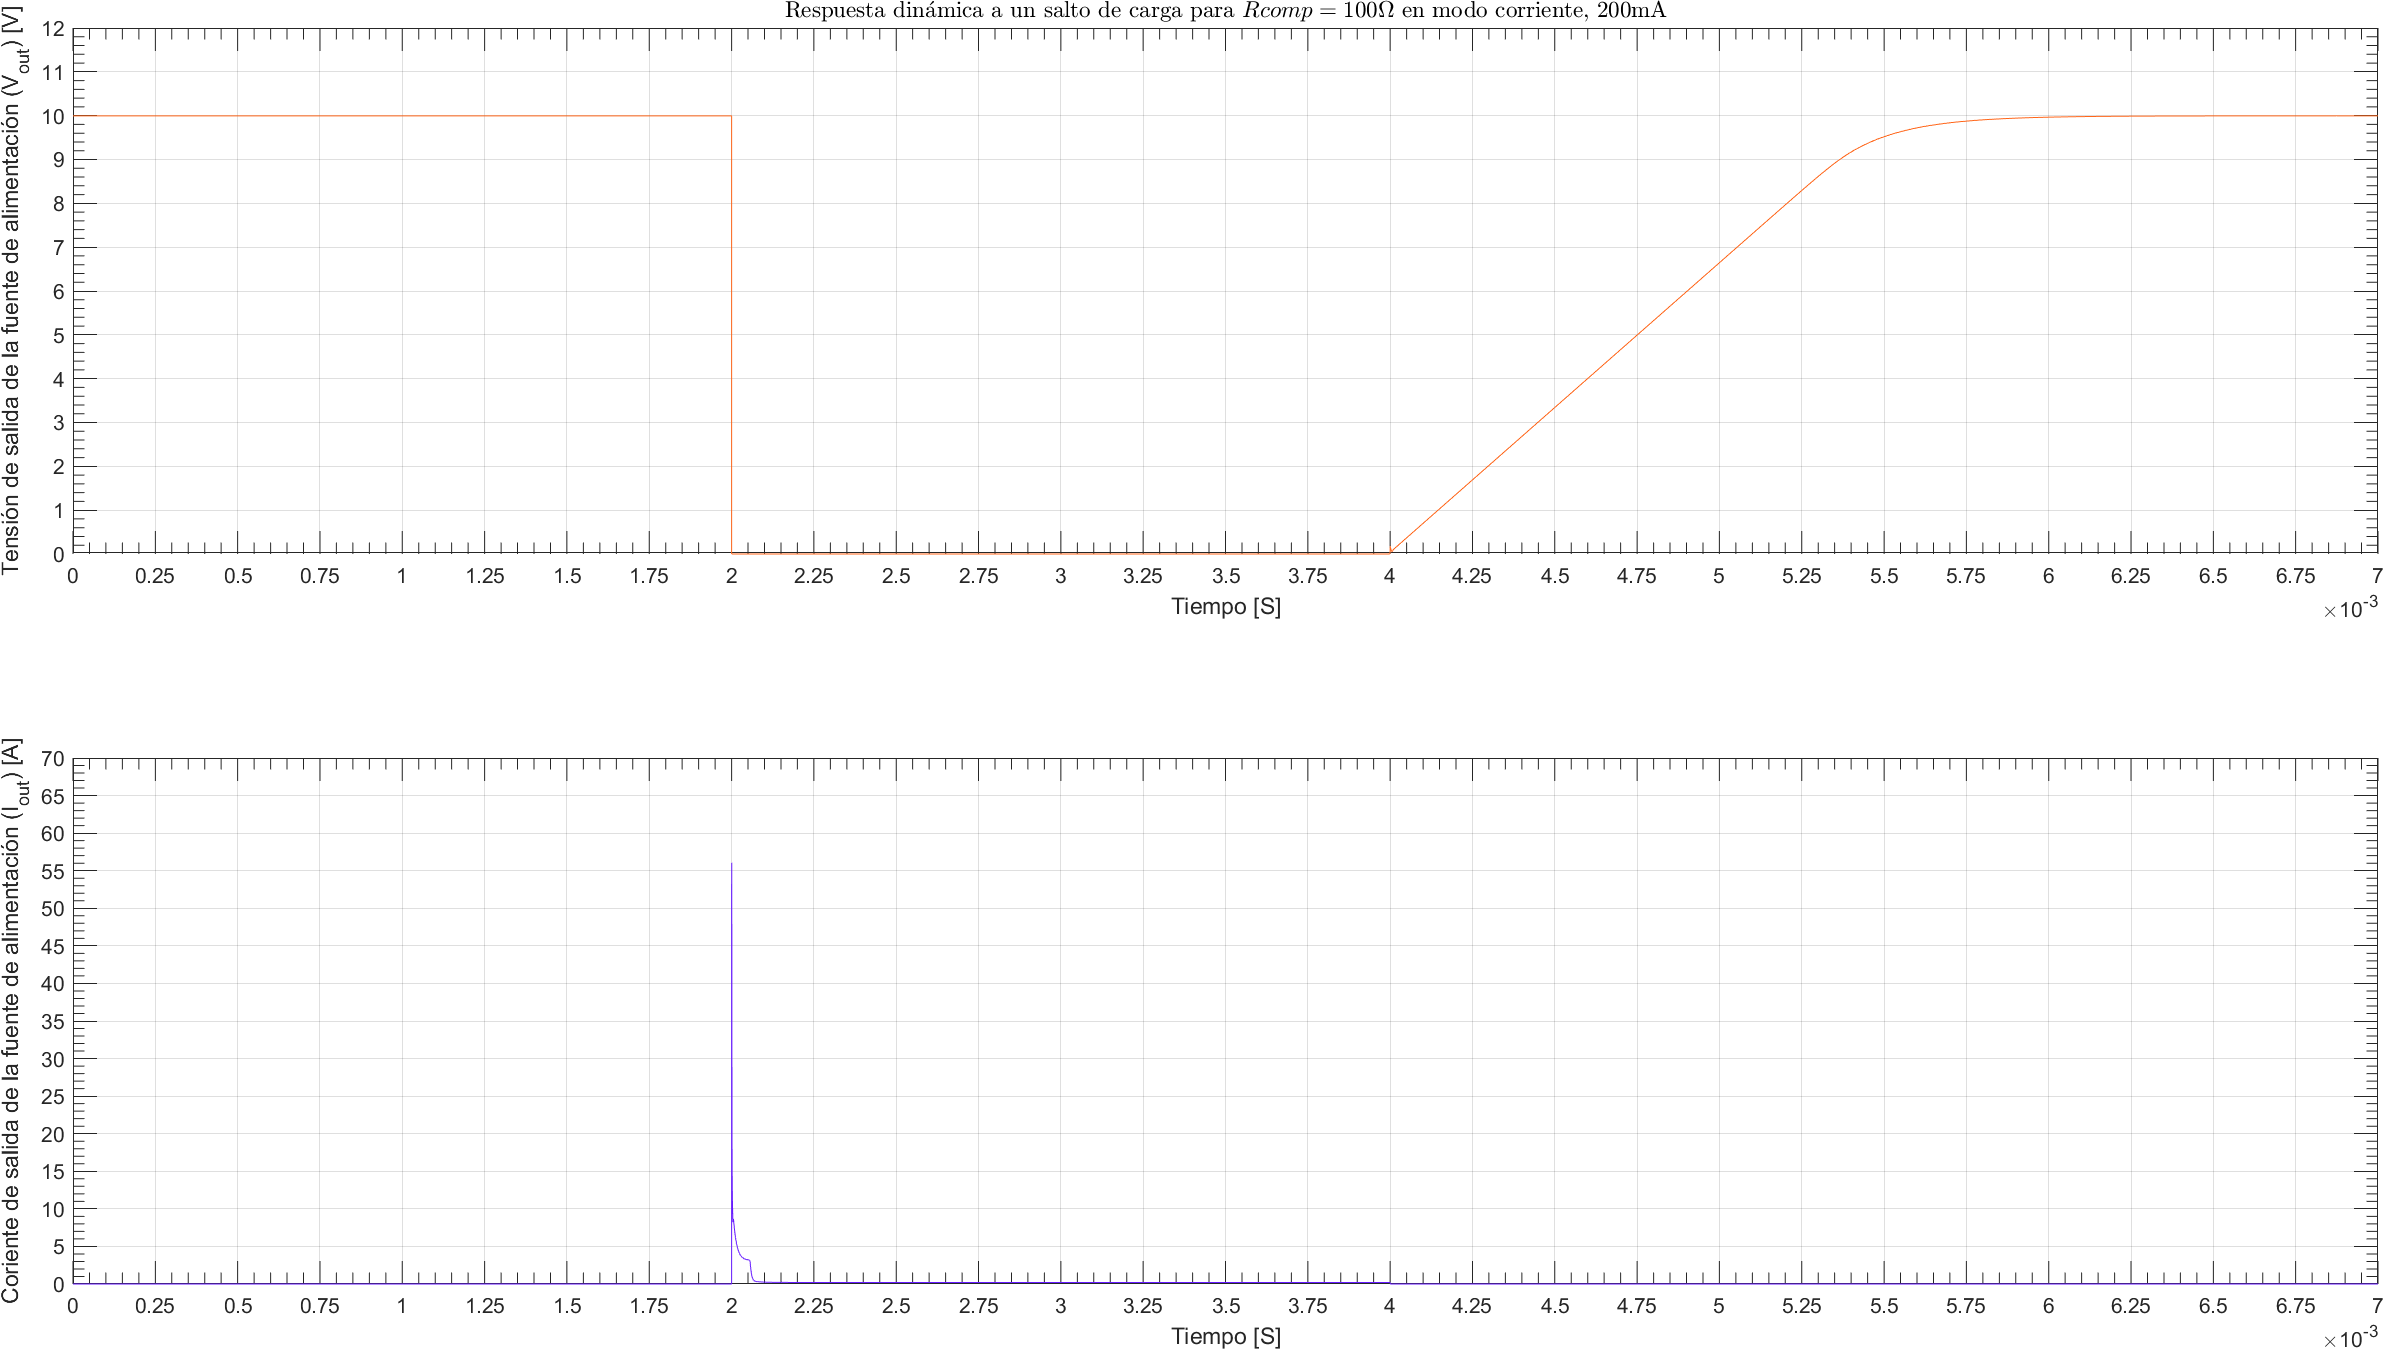
\includegraphics[width=1.1 \textwidth, angle=90]{./img/plots/dynamic/power_supply_RCOMP_100_STEP_Modo4.png}
\caption{\label{fig:fig_power_supply_RCOMP_STEP_100_Modo4}\footnotesize{Respuesta dinámica en modo corriente, $I_{out} = 200 \si[per-mode=symbol]{\milli\ampere}$, para $R_{comp} = 100 \si[per-mode=symbol]{\ohm} $.}}
\end{center}
\end{figure}

\clearpage







\clearpage
%\\\\\\\\\\\\\\\\\\\\\\\\\\\


%\\\\\\\\\\\\\\\\\\\\\\\\\\\
\subsection{Red de compensación de $C_{comp_{2}}$}

La red que contiene a $\bm{C_{comp2}}$ actúa solo para el lazo de tensión, por lo que se analiza solo este modo.



\subsubsection{Análisis para $C_{comp_{2}}$ en modo tensión, $V_{out} = 10 \si[per-mode=symbol]{\volt}$, $R_{L} = 2 \si[per-mode=symbol]{\ohm}$}

Se puede ver en la figura~\figref{fig:fig_power_supply_CCOMP2_LOOP_Modo1} como ya con el valor de $C_{comp_{2}} = 2 \si[per-mode=symbol]{\nano\farad}$ se logra unos márgenes de fase y ganancia aceptables, valores menores o mayores los disminuyen, además seguir aumentando el valor de $C_{comp_{2}}$, solo disminuye innecesariamente el ancho de banda, como se puede ver en la figura~\figref{fig:fig_power_supply_CCOMP2_RF_Modo1}. A nivel de respuesta dinámica no se ven grandes diferencias entre los valores simulados, ver figura~\figref{fig:fig_power_supply_CCOMP2_STEP_0_Modo1}, figura~\figref{fig:fig_power_supply_CCOMP2_STEP_2n_Modo1} y figura~\figref{fig:fig_power_supply_CCOMP2_STEP_5n_Modo1}.

\vfill


% CCOMP2 MODO 1.

\clearpage

\begin{figure}[H] %htb
\begin{center}
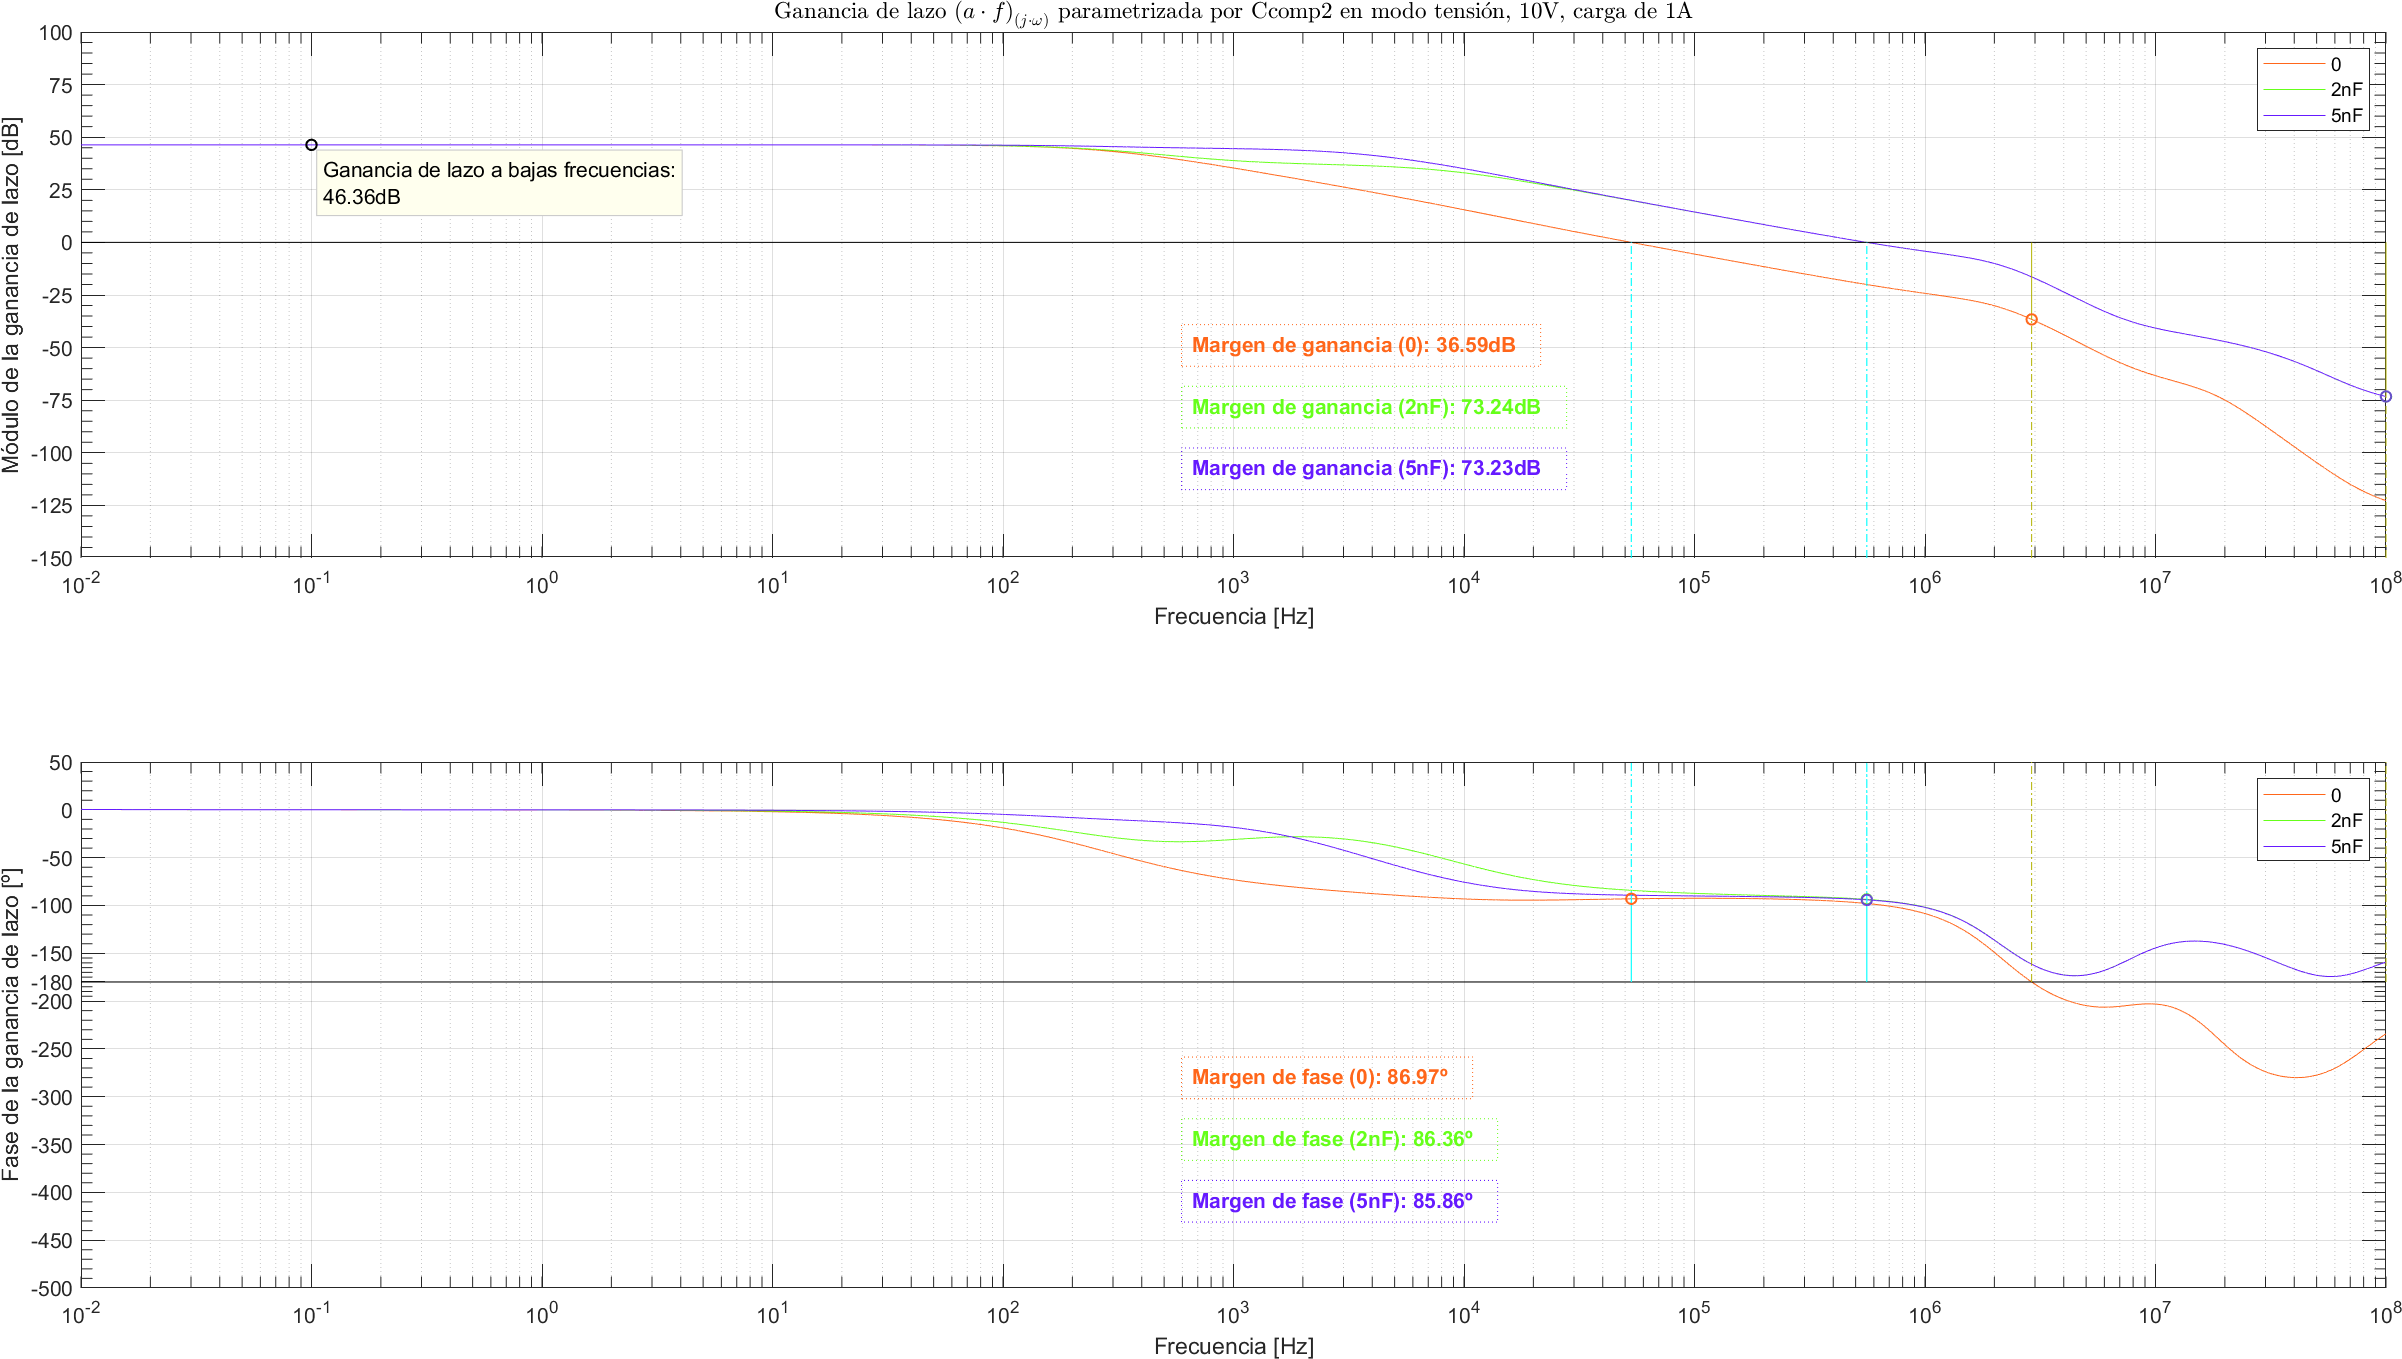
\includegraphics[width=1.1 \textwidth, angle=90]{./img/plots/loop/power_supply_CCOMP2_LOOP_Modo1.png}
\caption{\label{fig:fig_power_supply_CCOMP2_LOOP_Modo1}\footnotesize{Ganancia de lazo en modo tensión, $V_{out} = 10 \si[per-mode=symbol]{\volt}$, en función de la frecuencia parametrizada por $C_{comp_{2}}$.}}
\end{center}
\end{figure}


\clearpage

\begin{figure}[H] %htb
\begin{center}
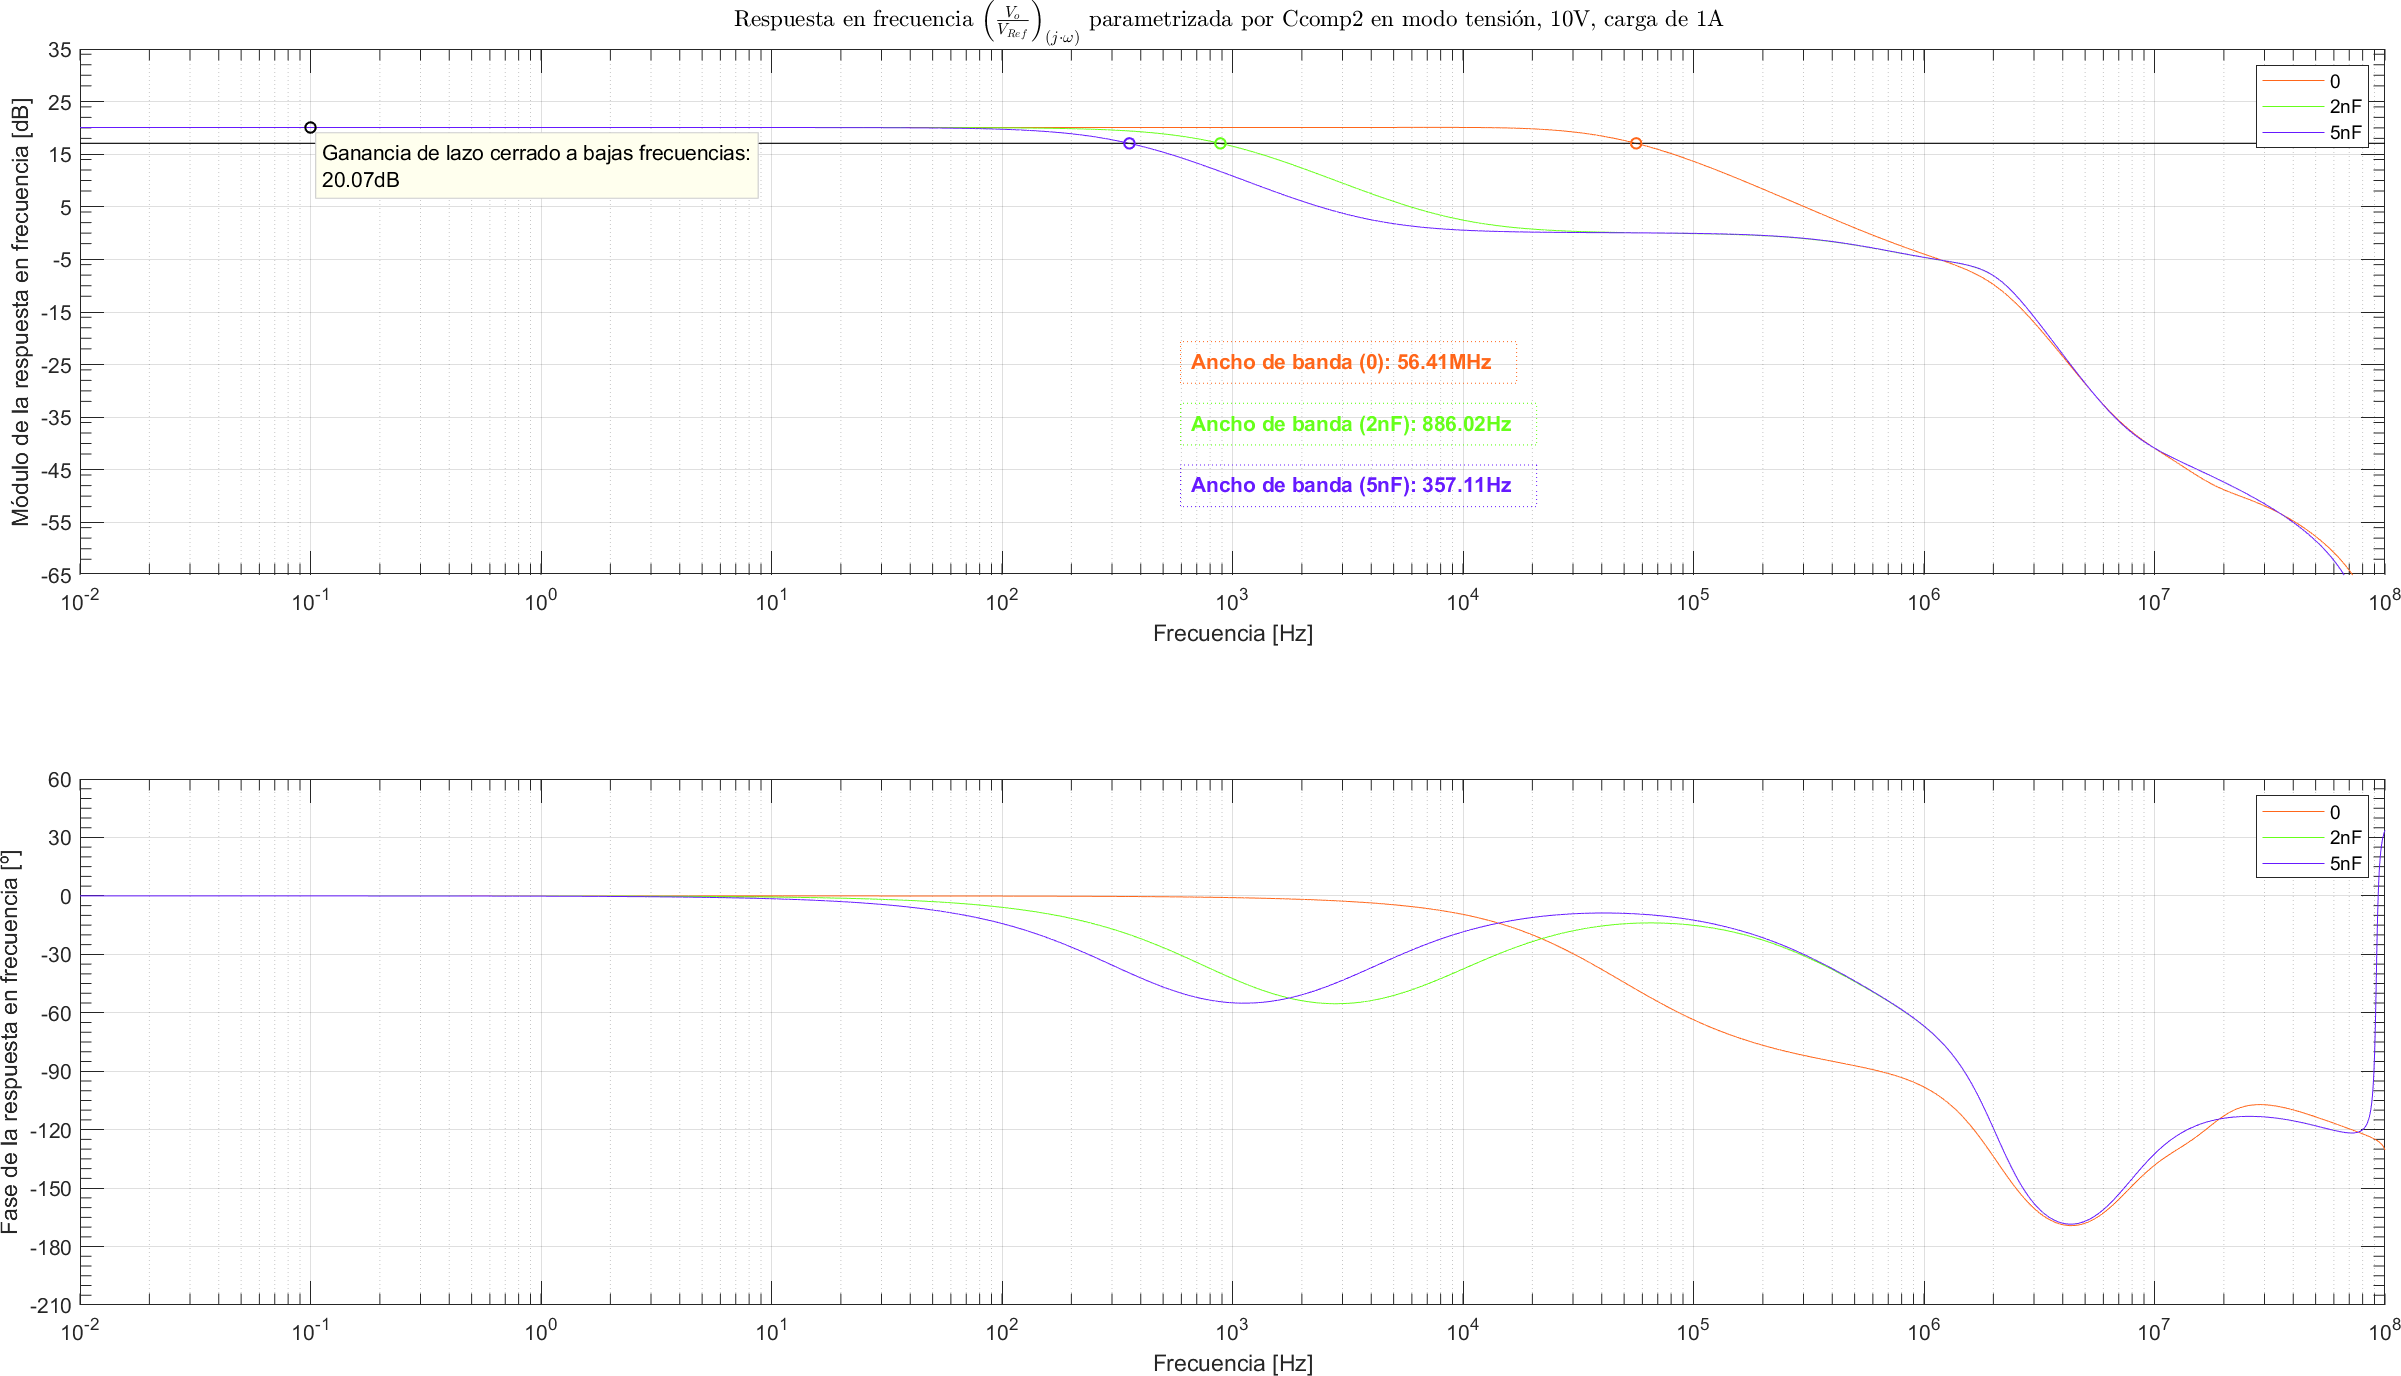
\includegraphics[width=1.1 \textwidth, angle=90]{./img/plots/rf/power_supply_CCOMP2_RF_Modo1.png}
\caption{\label{fig:fig_power_supply_CCOMP2_RF_Modo1}\footnotesize{Respuesta en frecuencia en modo tensión, $V_{out} = 10 \si[per-mode=symbol]{\volt}$, en función de la frecuencia parametrizada por $C_{comp_{2}}$.}}
\end{center}
\end{figure}

\clearpage

\begin{figure}[H] %htb
\begin{center}
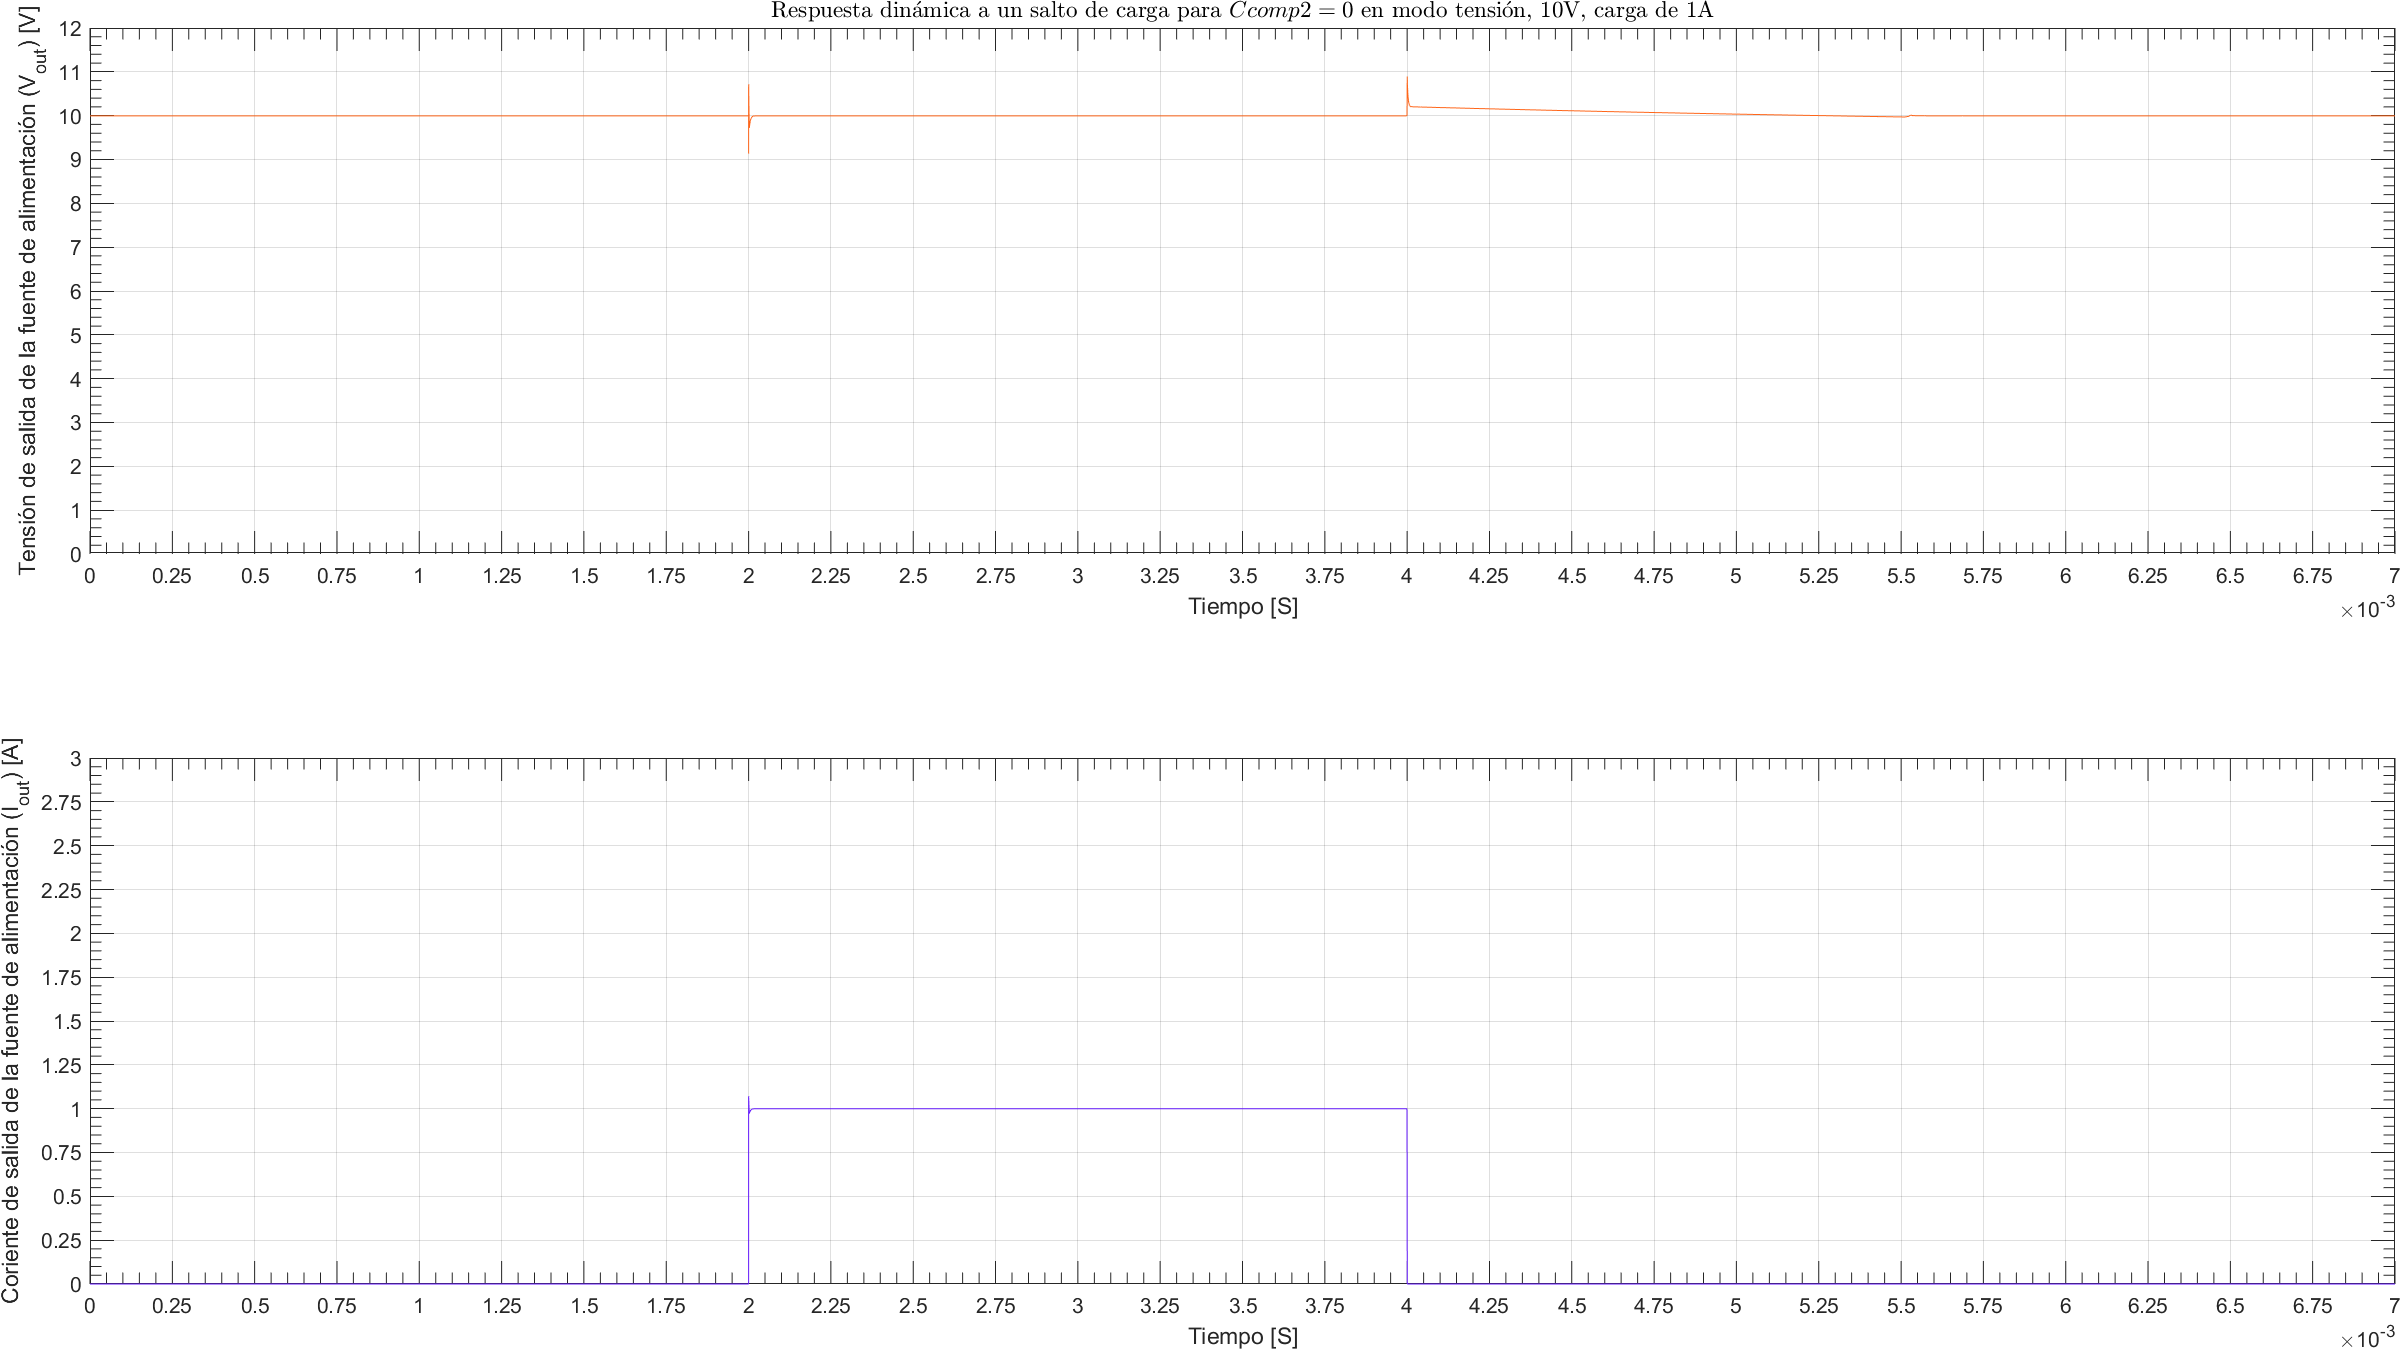
\includegraphics[width=1.1 \textwidth, angle=90]{./img/plots/dynamic/power_supply_CCOMP2_0_STEP_Modo1.png}
\caption{\label{fig:fig_power_supply_CCOMP2_STEP_0_Modo1}\footnotesize{Respuesta dinámica en modo tensión, $V_{out} = 10 \si[per-mode=symbol]{\volt}$, para $C_{comp_{2}} = 0 \si[per-mode=symbol]{\nano\farad} $.}}
\end{center}
\end{figure}

\clearpage

\begin{figure}[H] %htb
\begin{center}
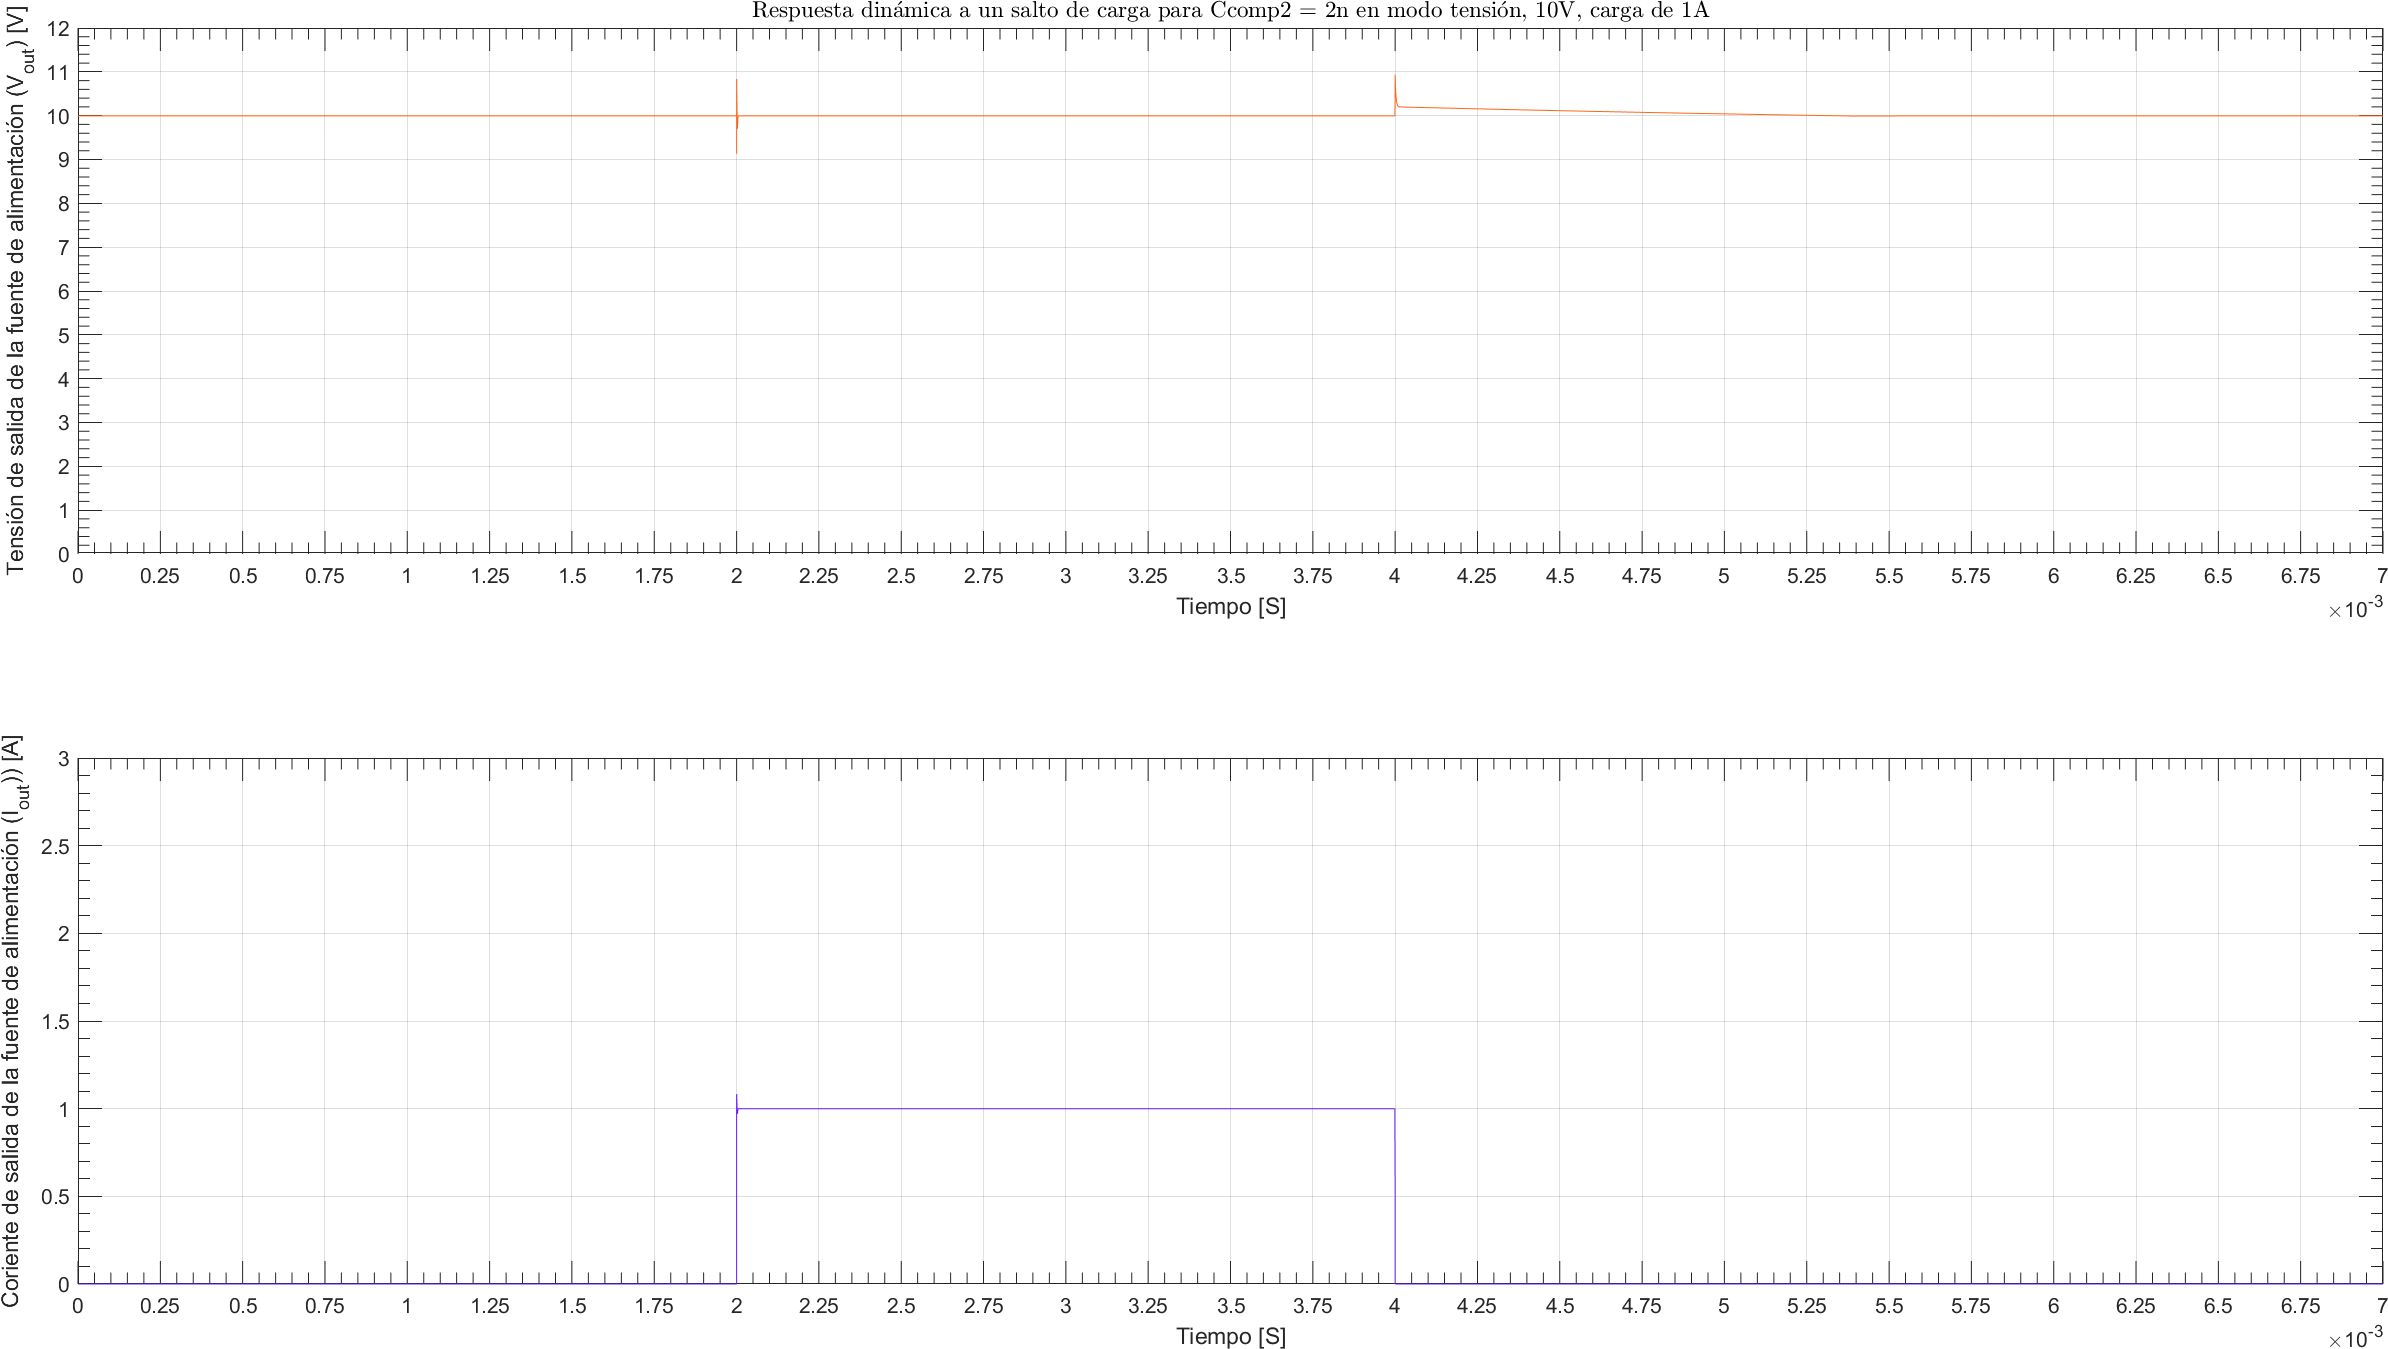
\includegraphics[width=1.1 \textwidth, angle=90]{./img/plots/dynamic/power_supply_CCOMP2_2n_STEP_Modo1.png}
\caption{\label{fig:fig_power_supply_CCOMP2_STEP_2n_Modo1}\footnotesize{Respuesta dinámica en modo tensión, $V_{out} = 10 \si[per-mode=symbol]{\volt}$, para $C_{comp_{2}} = 2 \si[per-mode=symbol]{\nano\farad} $.}}
\end{center}
\end{figure}

\clearpage

\begin{figure}[H] %htb
\begin{center}
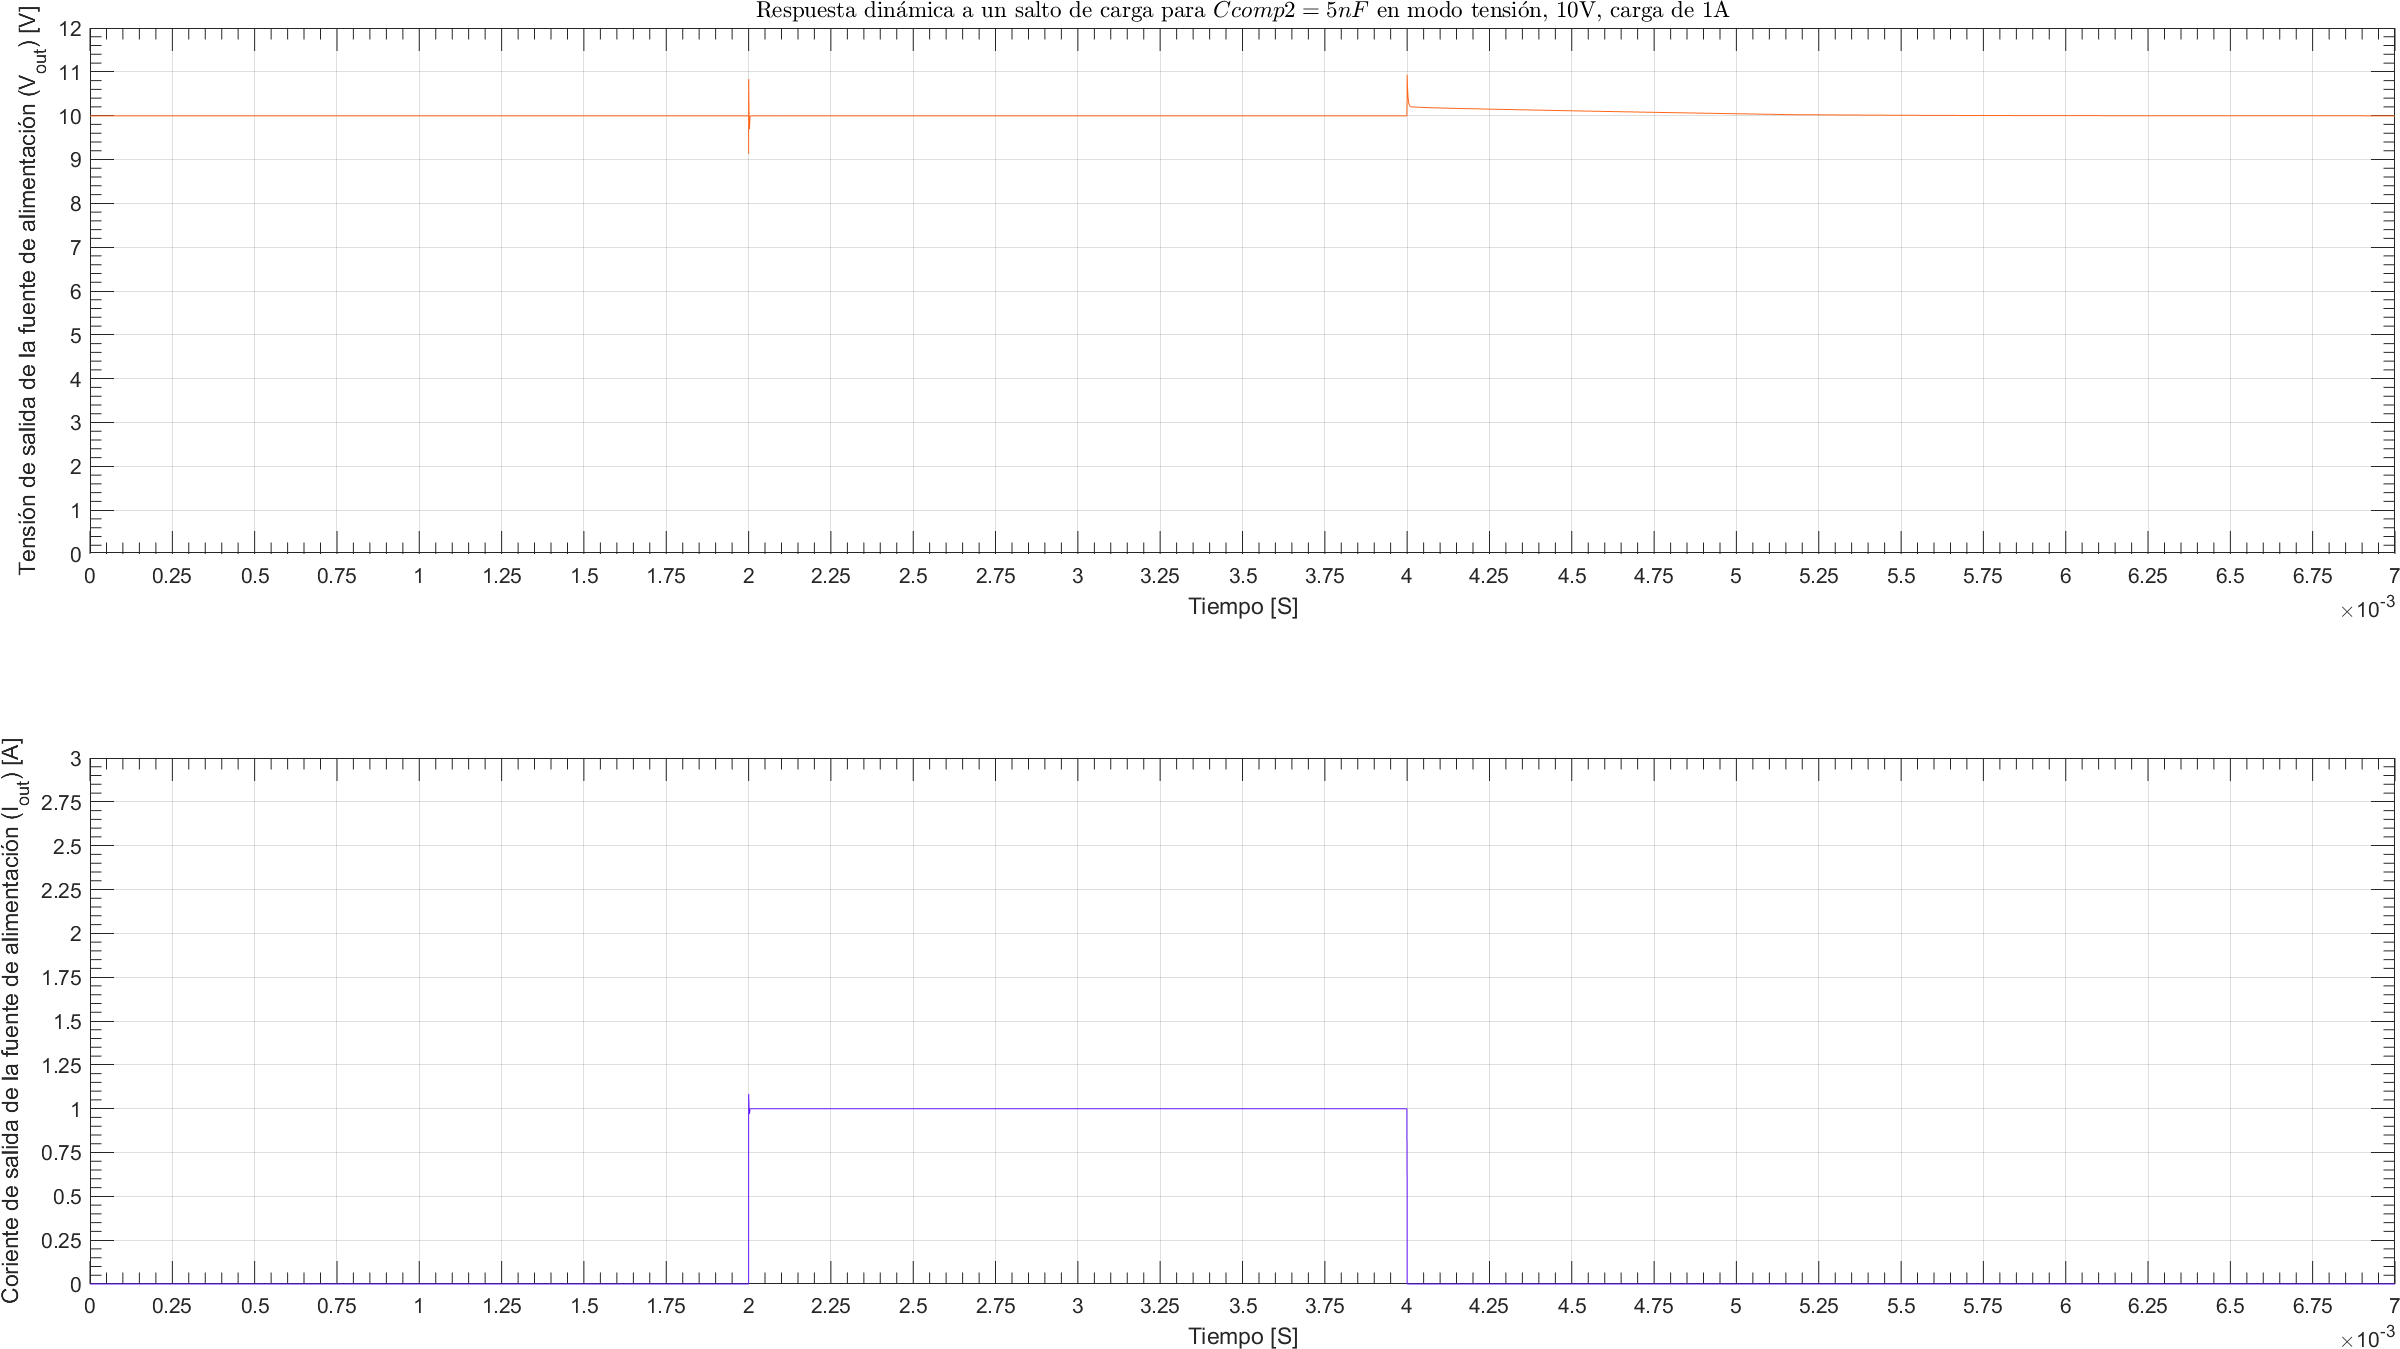
\includegraphics[width=1.1 \textwidth, angle=90]{./img/plots/dynamic/power_supply_CCOMP2_5n_STEP_Modo1.png}
\caption{\label{fig:fig_power_supply_CCOMP2_STEP_5n_Modo1}\footnotesize{Respuesta dinámica en modo tensión, $V_{out} = 10 \si[per-mode=symbol]{\volt}$, para $C_{comp_{2}} = 5 \si[per-mode=symbol]{\nano\farad} $.}}
\end{center}
\end{figure}

\clearpage



\clearpage
%\\\\\\\\\\\\\\\\\\\\\\\\\\\


%\\\\\\\\\\\\\\\\\\\\\\\\\\\
\subsection{Red de compensación de $C_{comp_{3}}$}

La red que contiene a $\bm{C_{comp3}}$ actúa solo para el lazo de corriente, por lo que se analiza solo este modo.


\subsubsection{Análisis para $C_{comp_{3}}$ en modo corriente, $I_{out} = 2 \si[per-mode=symbol]{\ampere}$, $R_{L} = 0 \si[per-mode=symbol]{\ohm}$}
% CCOMP3 MODO 3.

\clearpage

\begin{figure}[H] %htb
\begin{center}
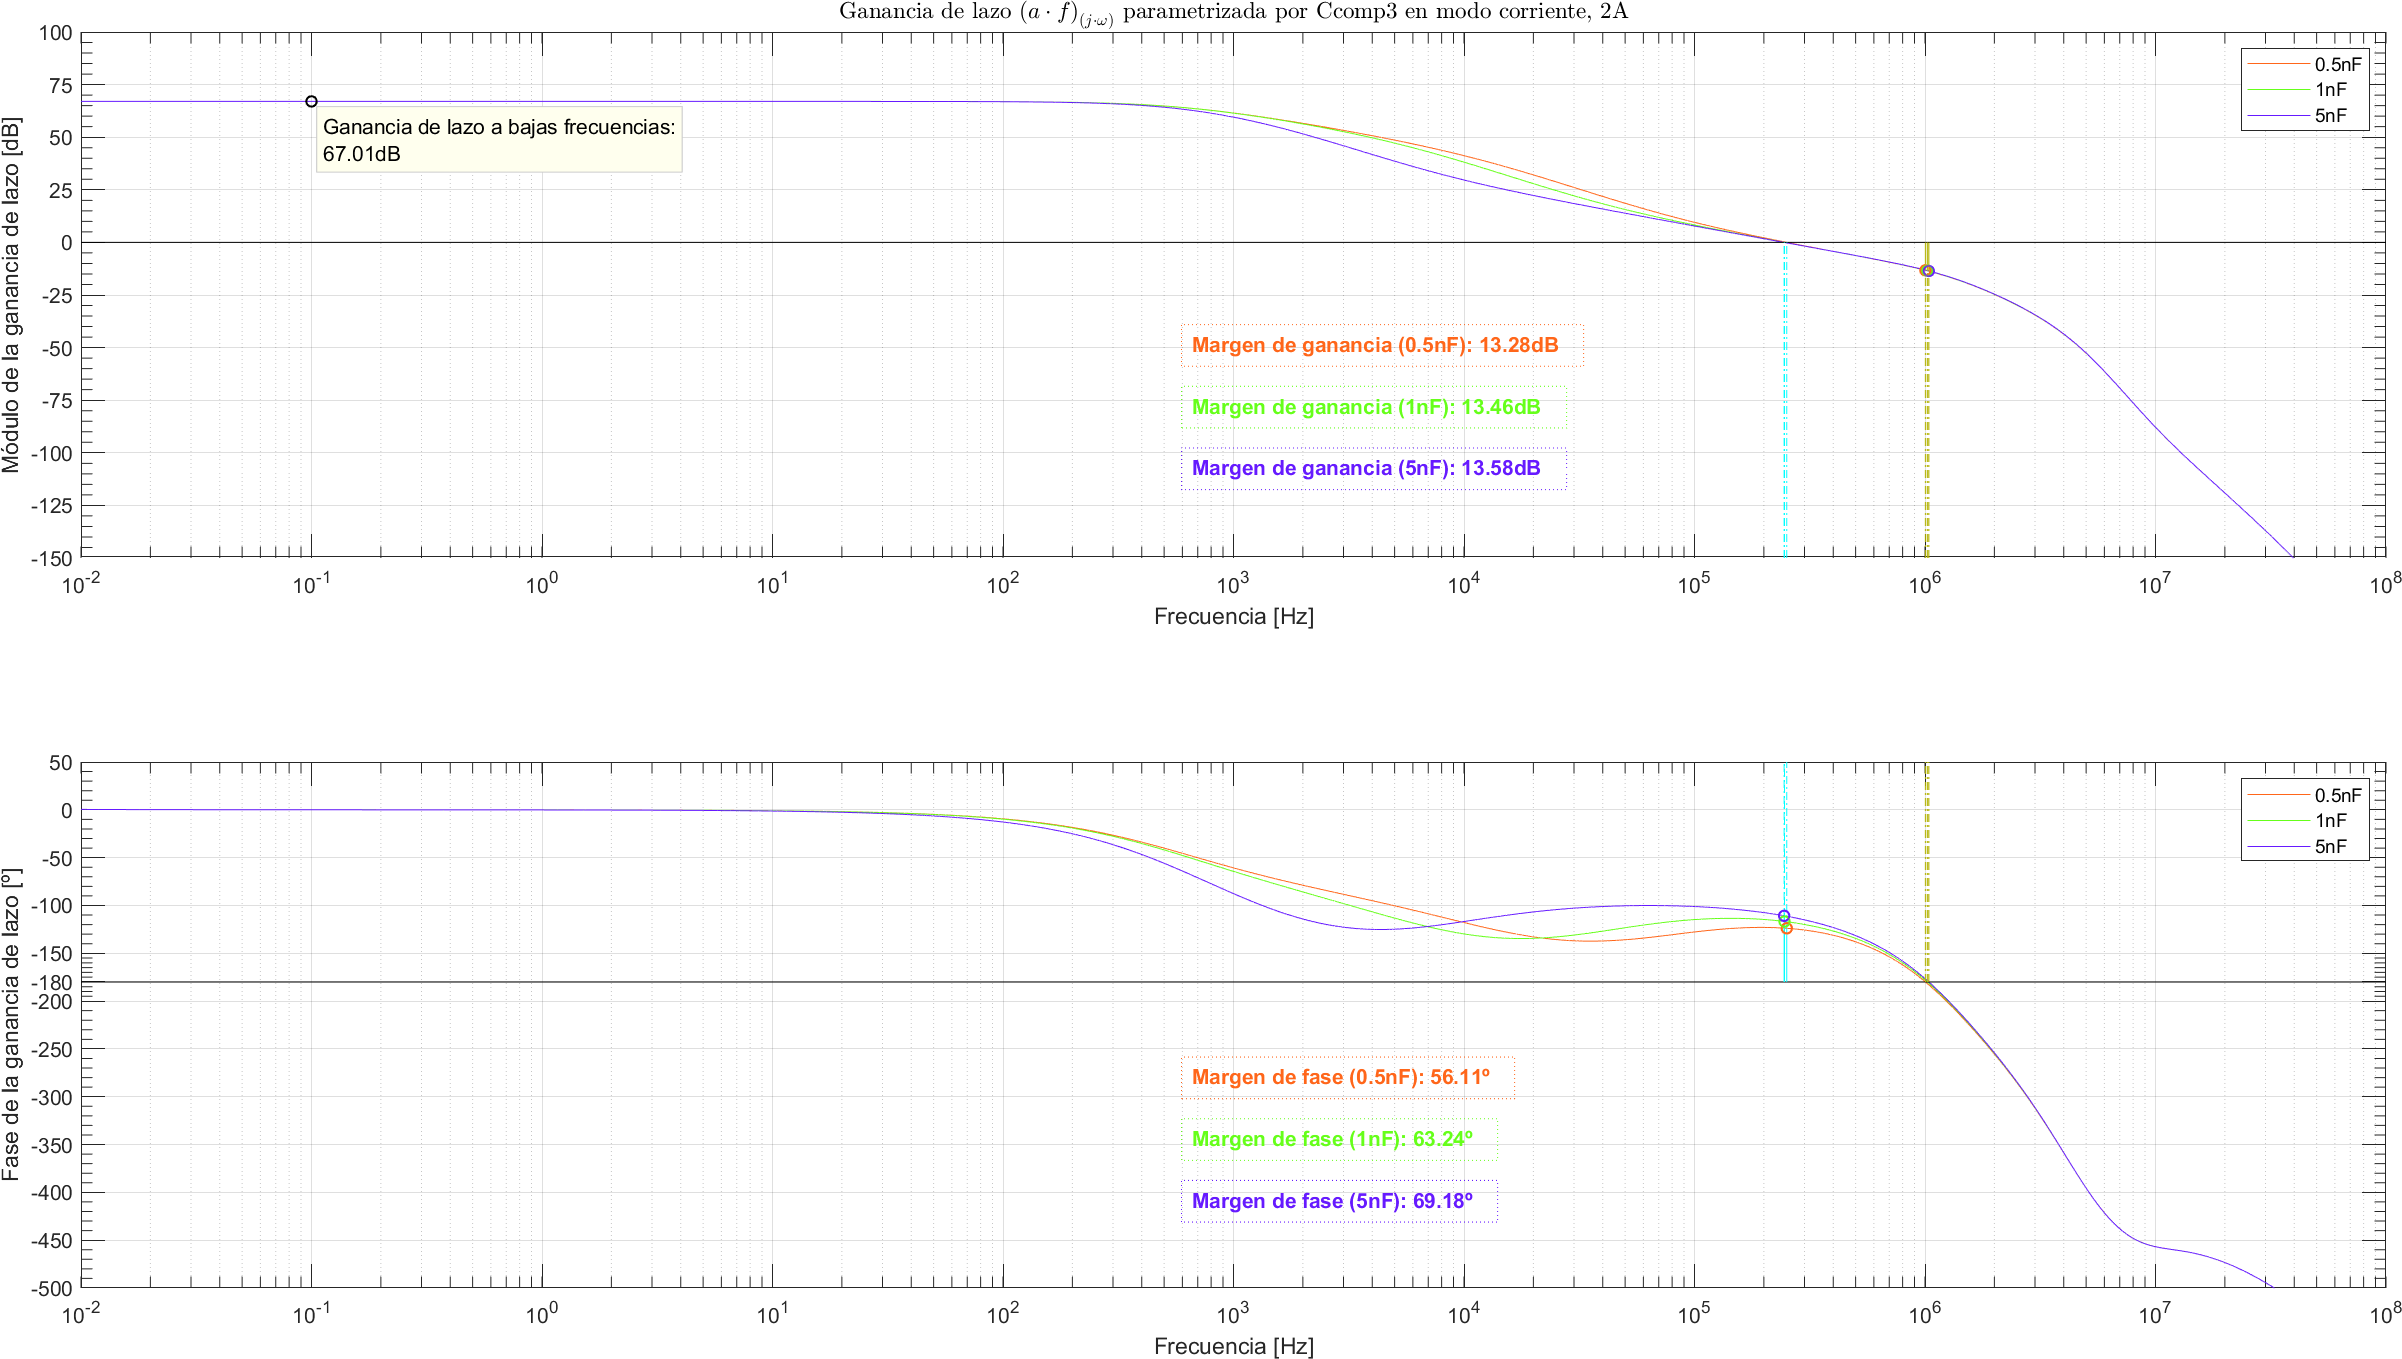
\includegraphics[width=1.1 \textwidth, angle=90]{./img/plots/loop/power_supply_CCOMP3_LOOP_Modo3.png}
\caption{\label{fig:fig_power_supply_CCOMP3_LOOP_Modo3}\footnotesize{Ganancia de lazo en modo corriente, $I_{out} = 2 \si[per-mode=symbol]{\ampere}$, en función de la frecuencia parametrizada por $C_{comp_{3}}$.}}
\end{center}
\end{figure}


\clearpage

\begin{figure}[H] %htb
\begin{center}
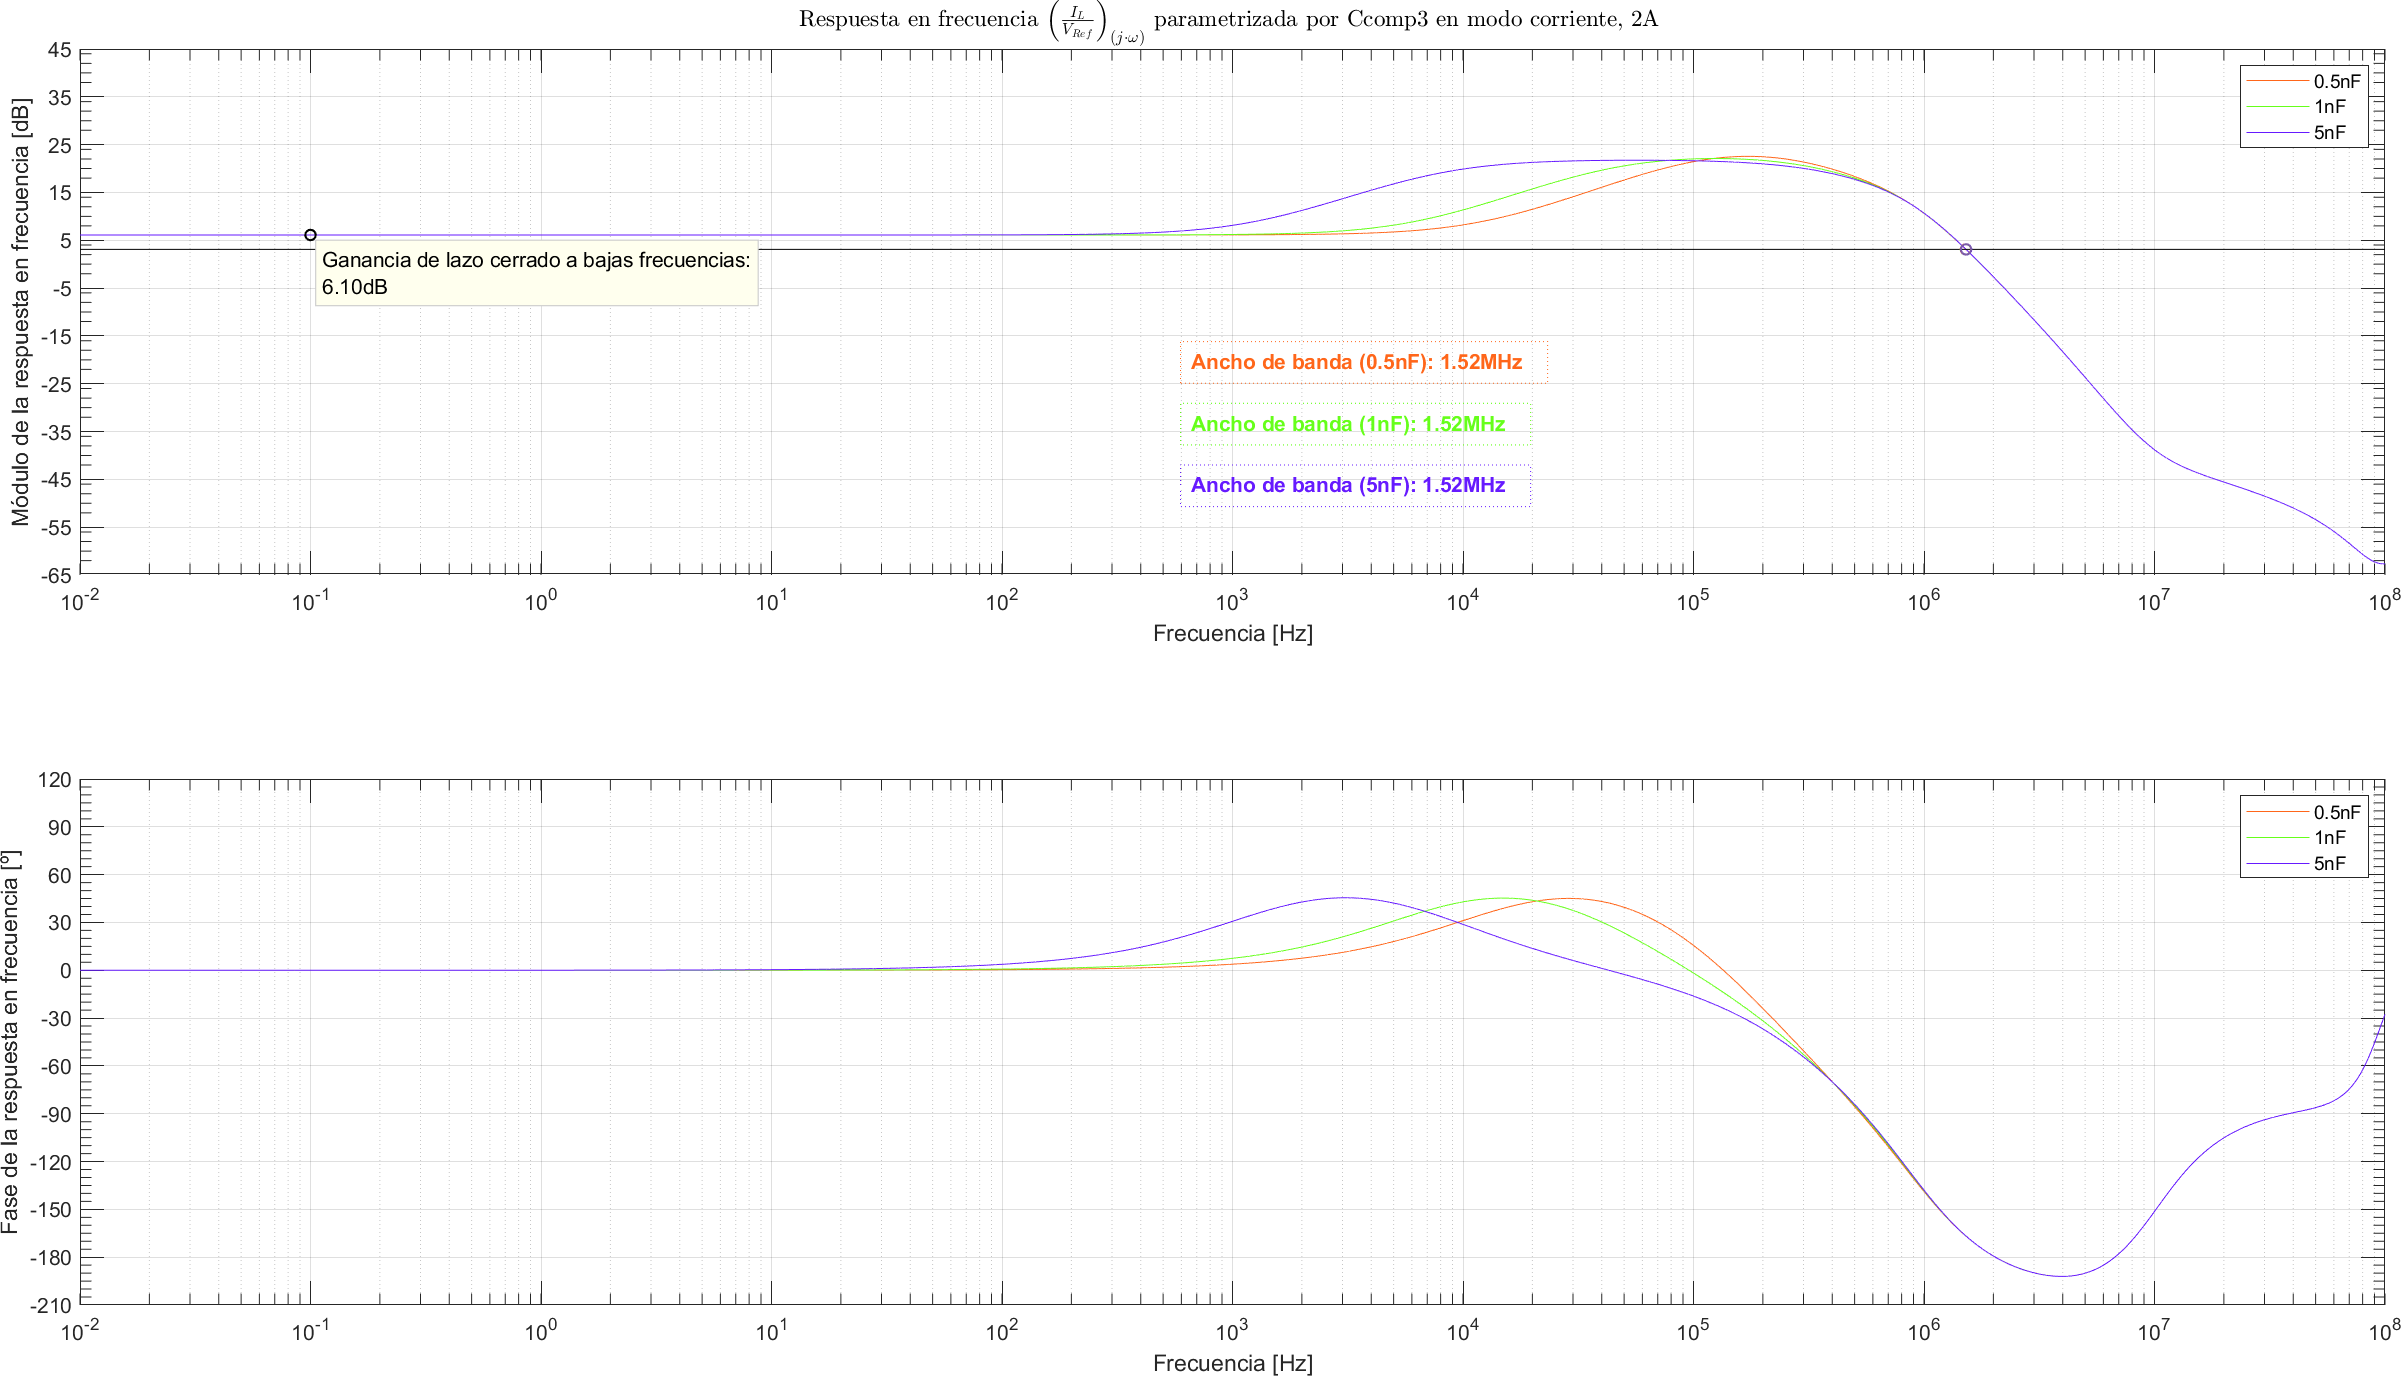
\includegraphics[width=1.1 \textwidth, angle=90]{./img/plots/rf/power_supply_CCOMP3_RF_Modo3.png}
\caption{\label{fig:fig_power_supply_CCOMP3_RF_Modo3}\footnotesize{Respuesta en frecuencia en modo corriente, $I_{out} = 2 \si[per-mode=symbol]{\ampere}$, en función de la frecuencia parametrizada por $C_{comp_{3}}$.}}
\end{center}
\end{figure}

\clearpage

\begin{figure}[H] %htb
\begin{center}
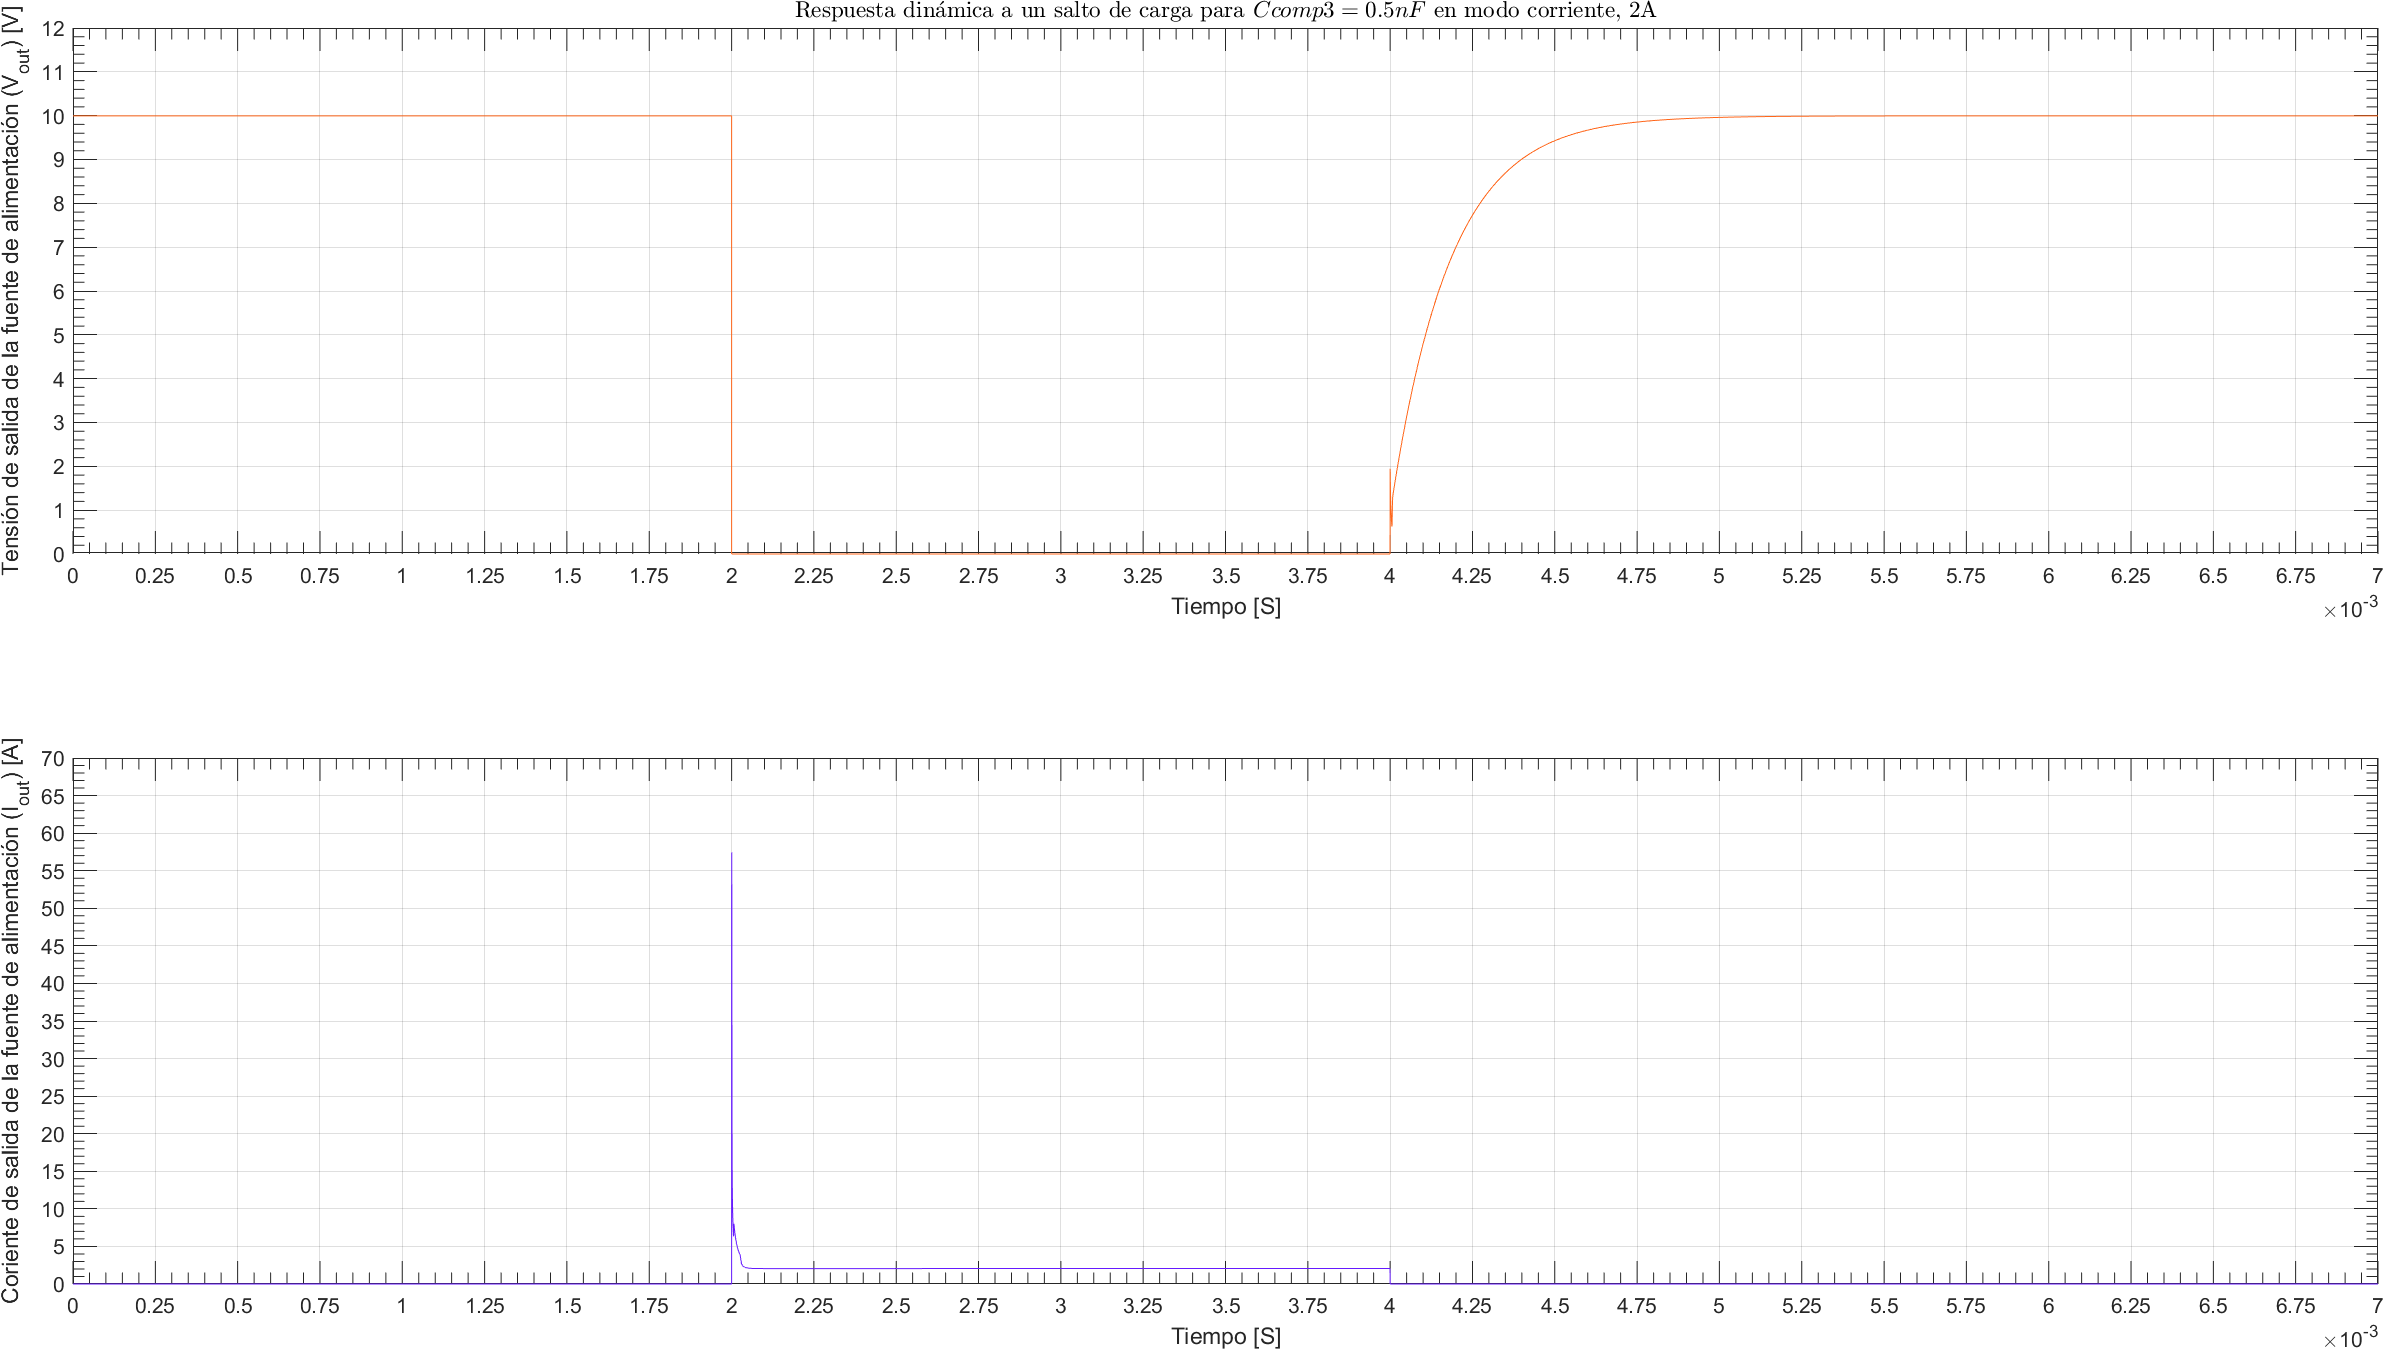
\includegraphics[width=1.1 \textwidth, angle=90]{./img/plots/dynamic/power_supply_CCOMP3_0_5n_STEP_Modo3.png}
\caption{\label{fig:fig_power_supply_CCOMP3_STEP_0_5n_Modo3}\footnotesize{Respuesta dinámica en modo corriente, $I_{out} = 2 \si[per-mode=symbol]{\ampere}$, para $C_{comp_{3}} = 0.5 \si[per-mode=symbol]{\nano\farad} $.}}
\end{center}
\end{figure}

\clearpage

\begin{figure}[H] %htb
\begin{center}
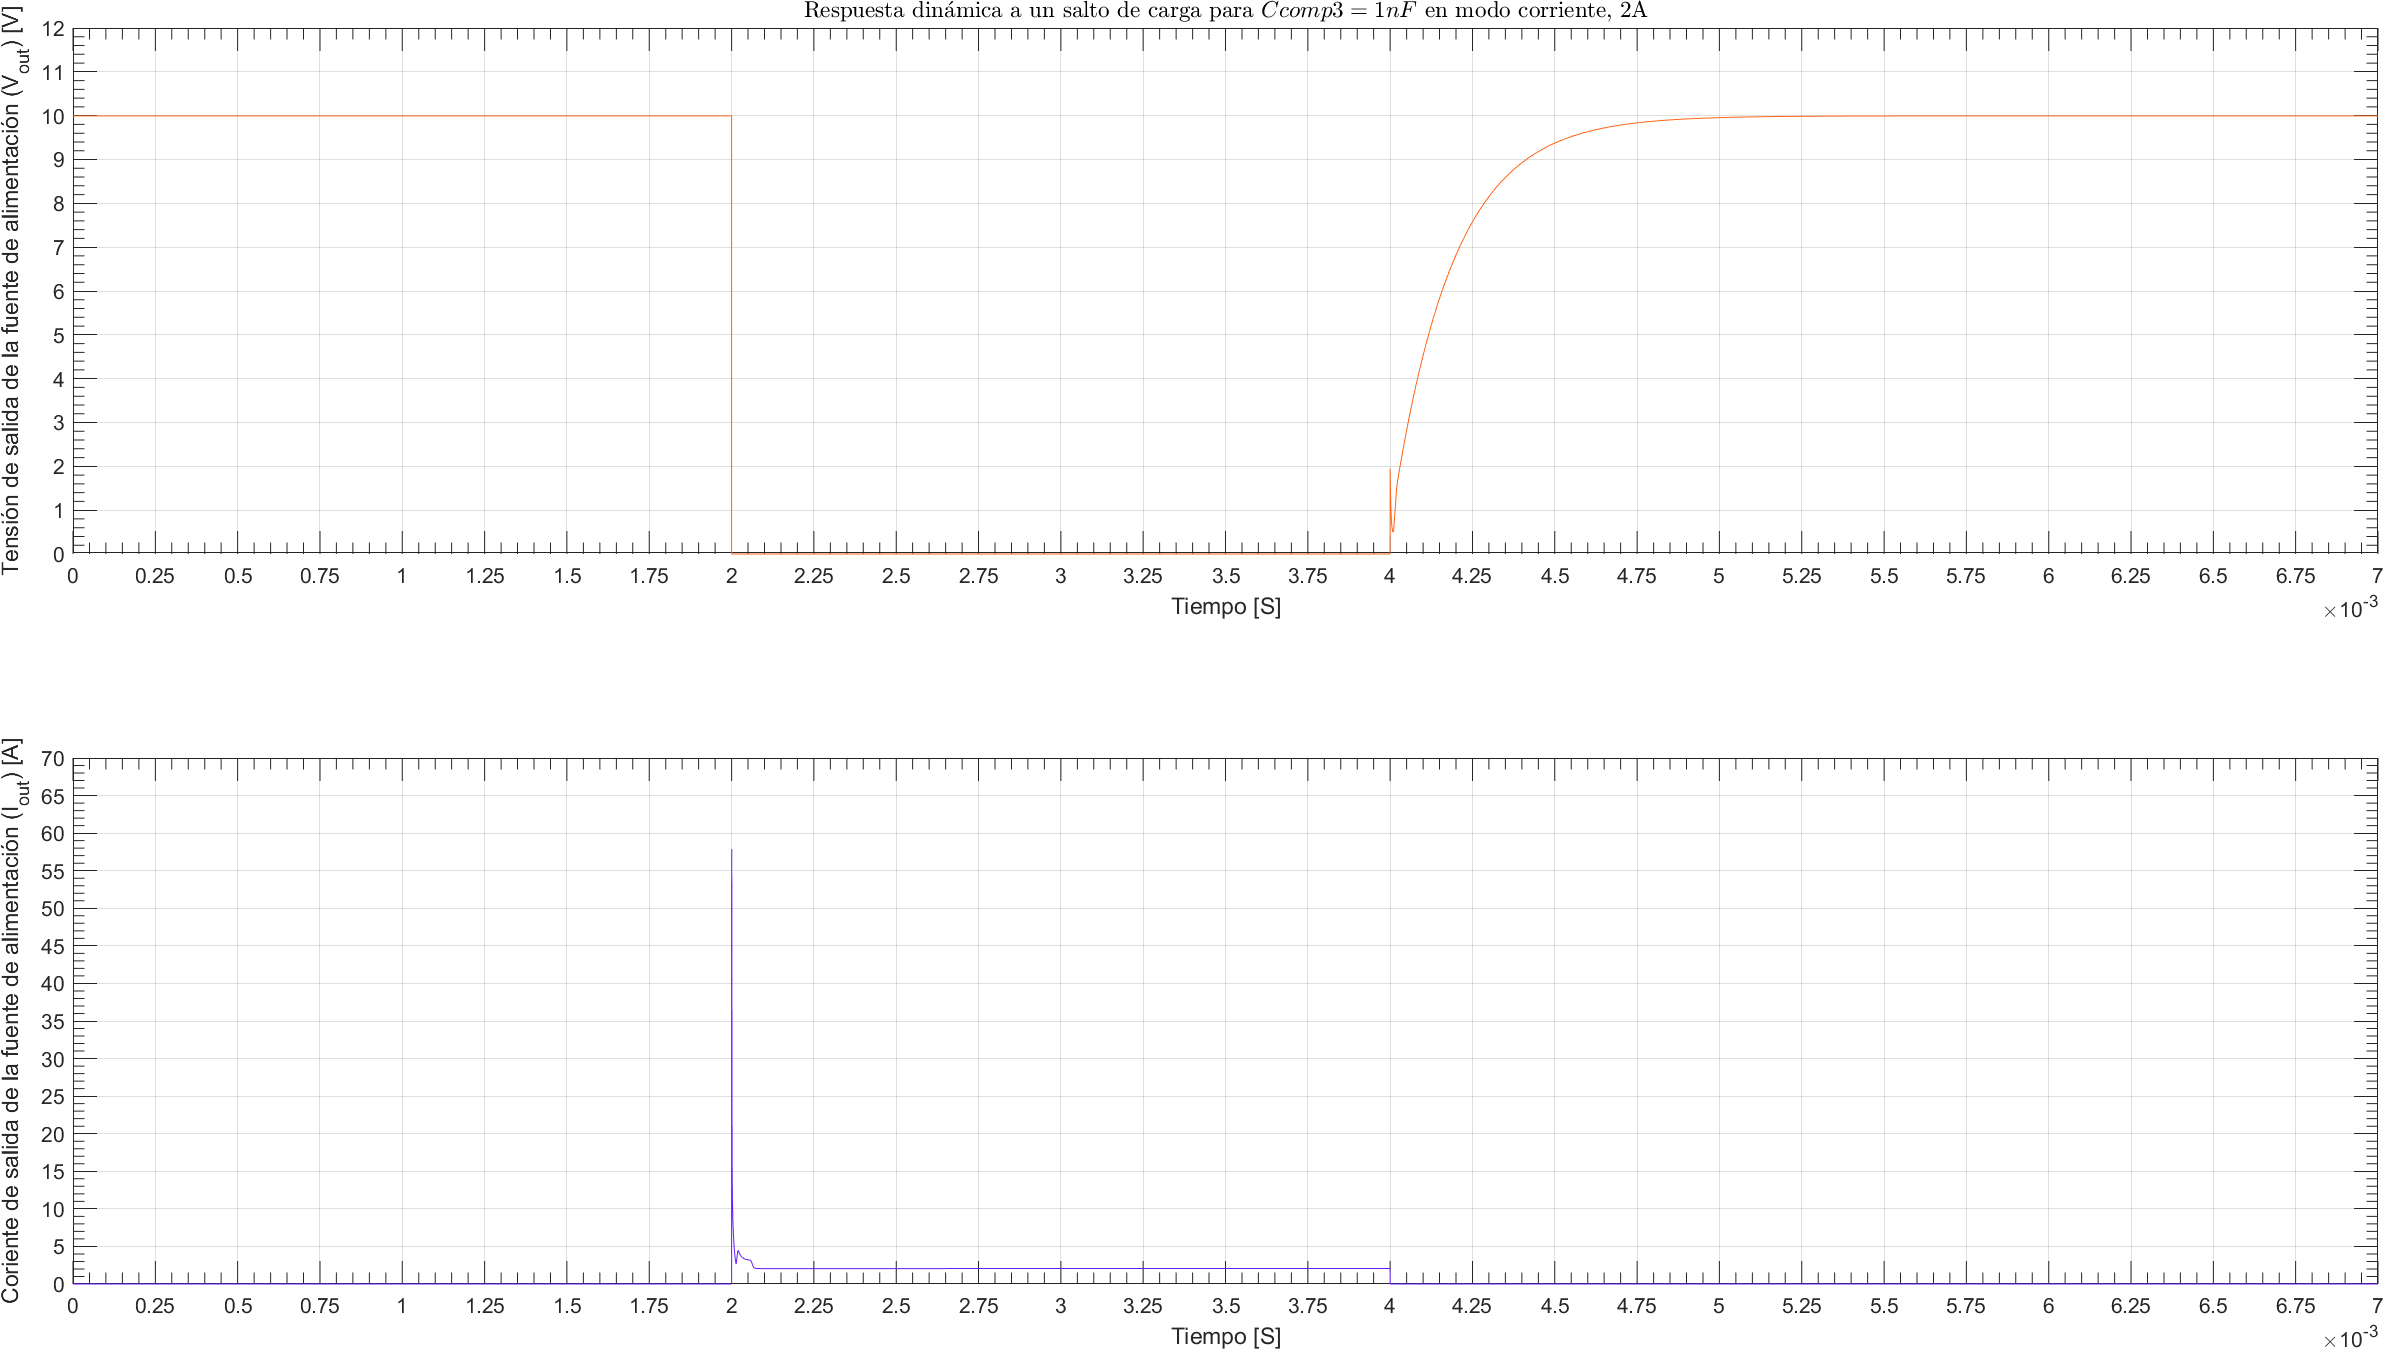
\includegraphics[width=1.1 \textwidth, angle=90]{./img/plots/dynamic/power_supply_CCOMP3_1n_STEP_Modo3.png}
\caption{\label{fig:fig_power_supply_CCOMP3_STEP_1n_Modo3}\footnotesize{Respuesta dinámica en modo corriente, $I_{out} = 2 \si[per-mode=symbol]{\ampere}$, para $C_{comp_{3}} = 1 \si[per-mode=symbol]{\nano\farad} $.}}
\end{center}
\end{figure}

\clearpage

\begin{figure}[H] %htb
\begin{center}
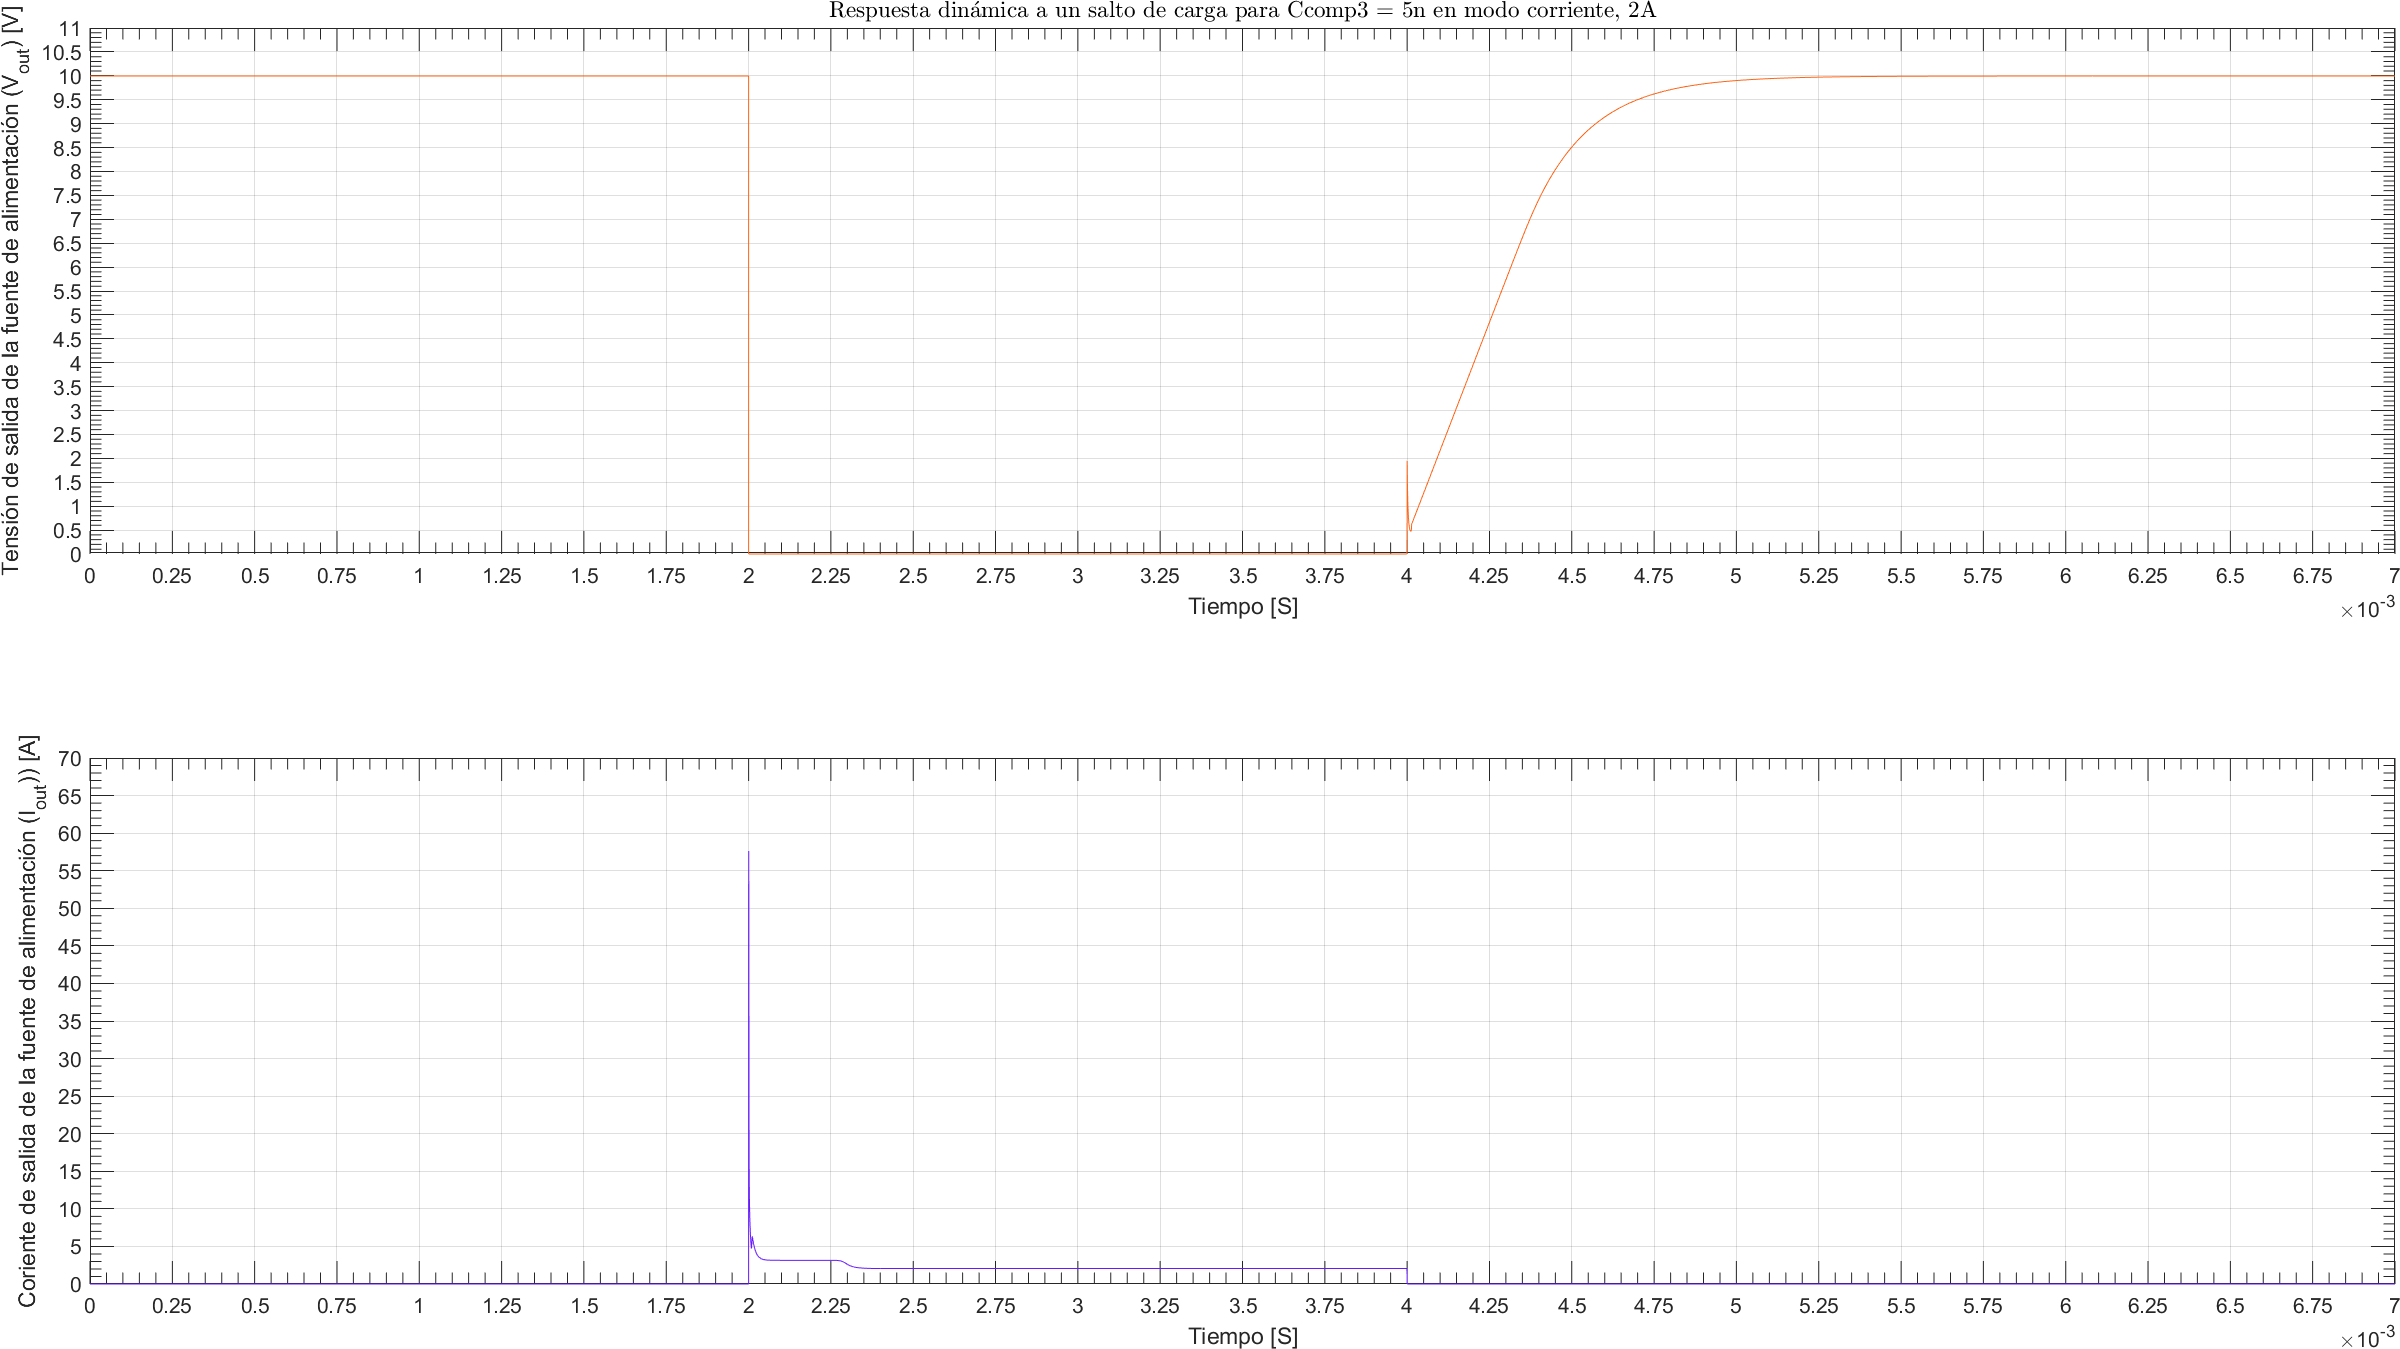
\includegraphics[width=1.1 \textwidth, angle=90]{./img/plots/dynamic/power_supply_CCOMP3_5n_STEP_Modo3.png}
\caption{\label{fig:fig_power_supply_CCOMP3_STEP_5n_Modo3}\footnotesize{Respuesta dinámica en modo corriente, $I_{out} = 2 \si[per-mode=symbol]{\ampere}$, para $C_{comp_{3}} = 5 \si[per-mode=symbol]{\nano\farad} $.}}
\end{center}
\end{figure}

\clearpage


\subsubsection{Análisis para $C_{comp_{3}}$ en modo corriente, $I_{out} = 200 \si[per-mode=symbol]{\milli\ampere}$, $R_{L} = 0 \si[per-mode=symbol]{\ohm}$}
% CCOMP3 MODO 4.

\clearpage

\begin{figure}[H] %htb
\begin{center}
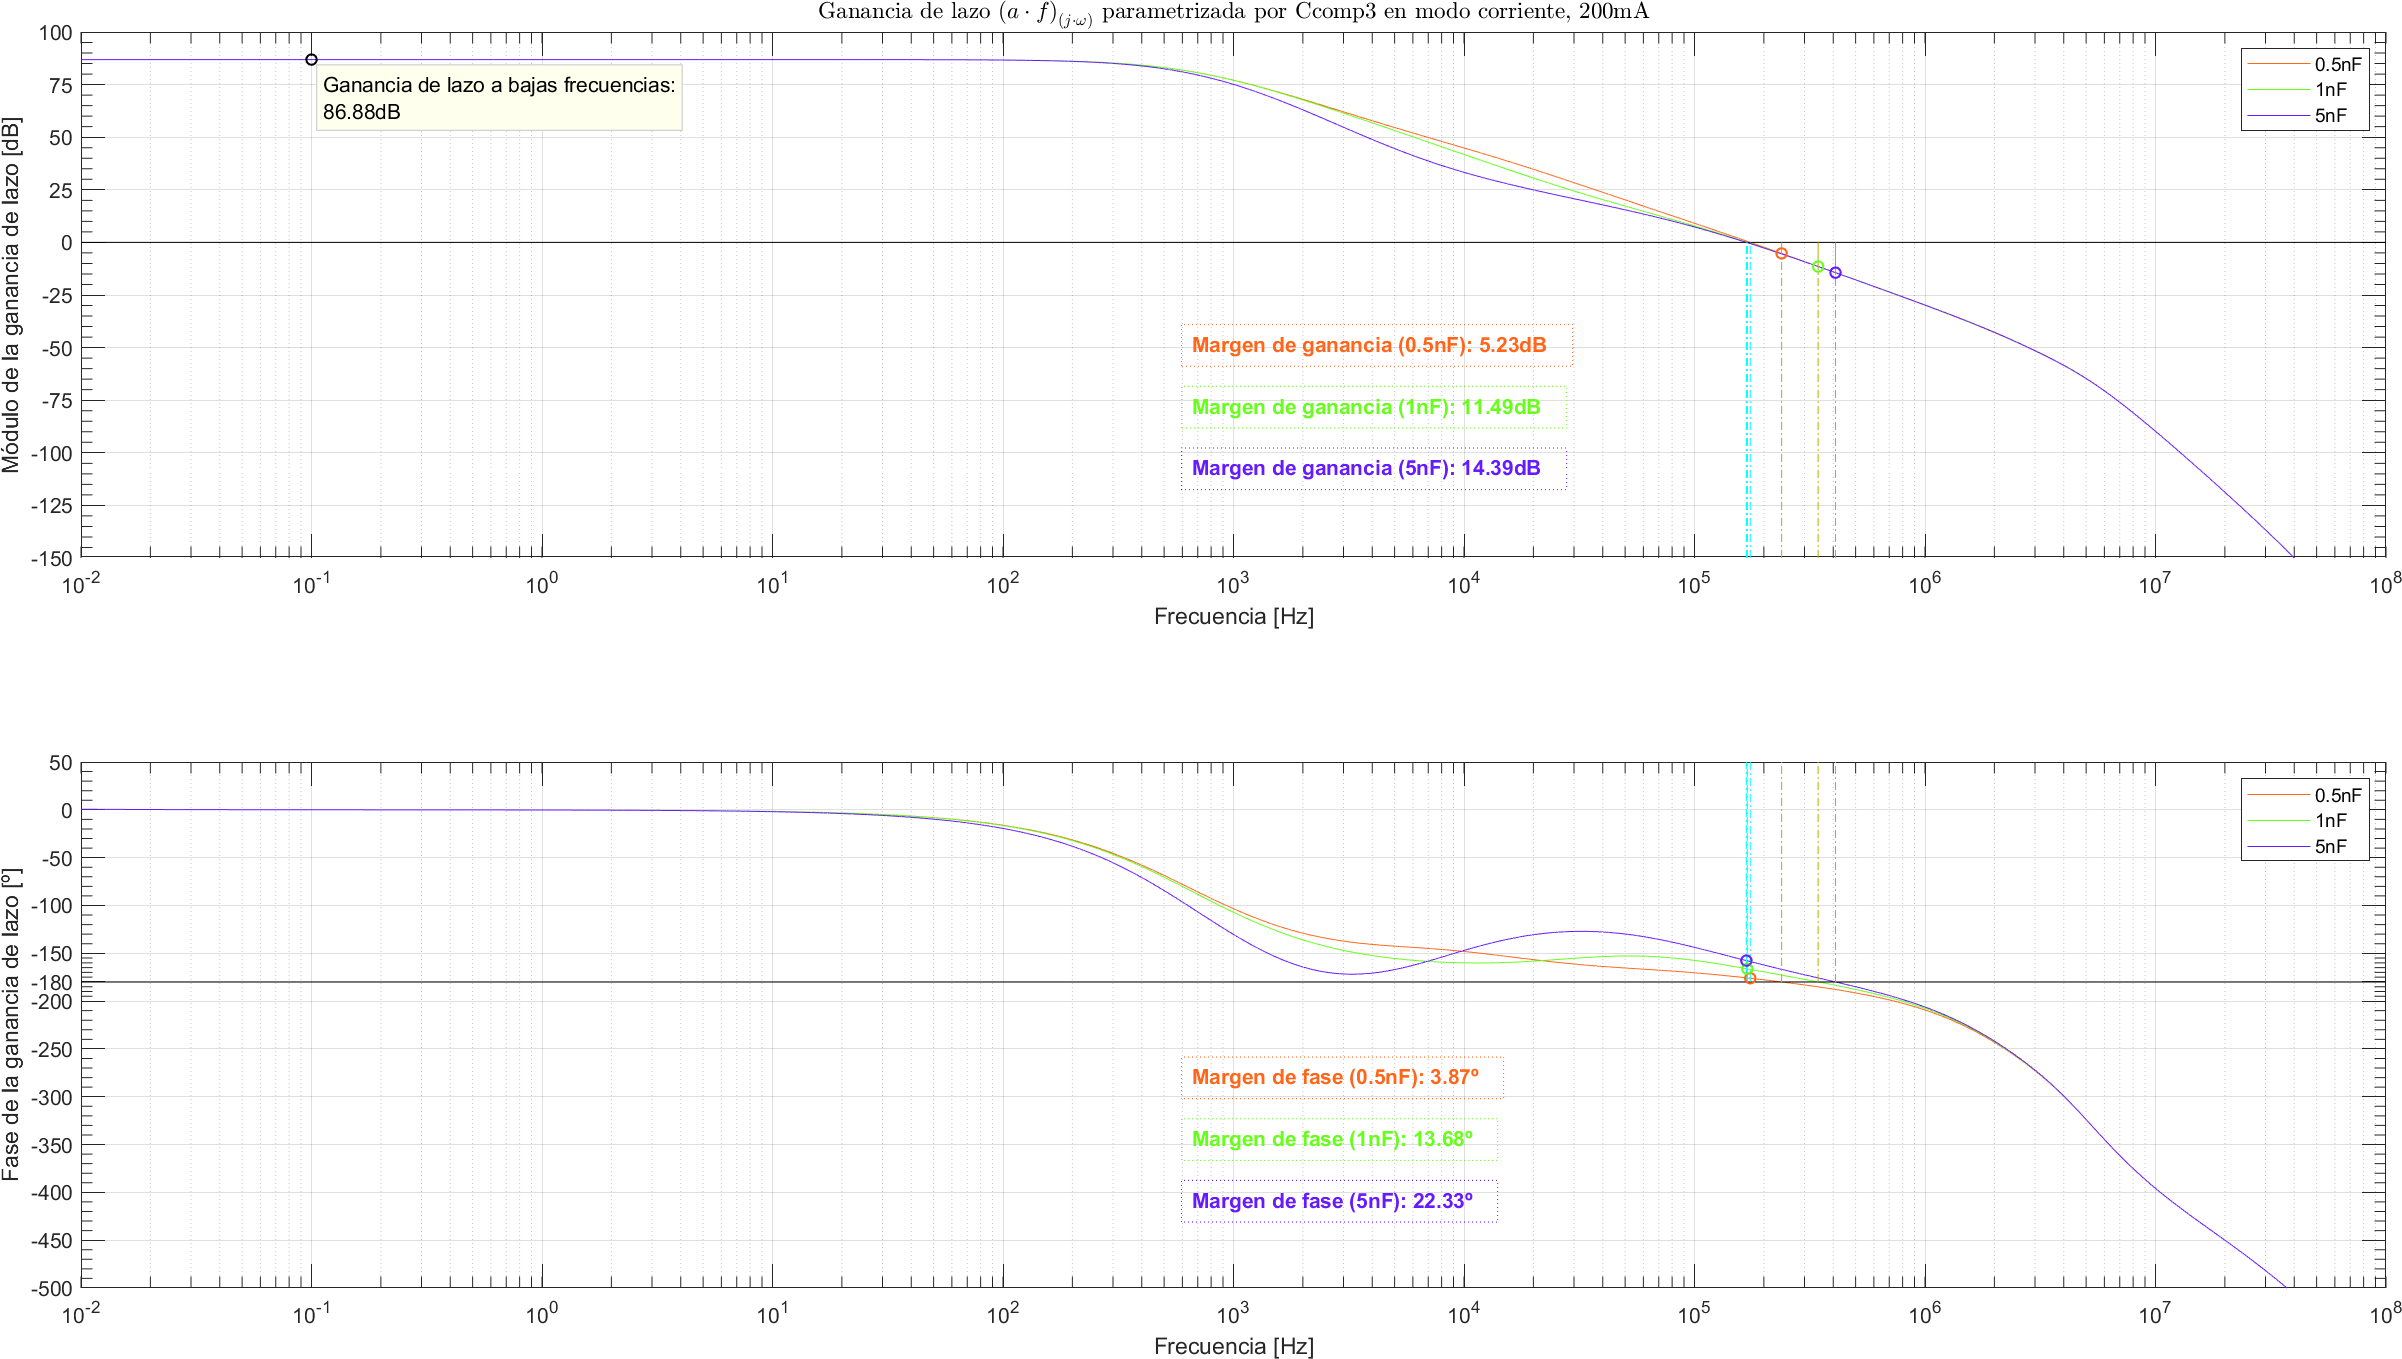
\includegraphics[width=1.1 \textwidth, angle=90]{./img/plots/loop/power_supply_CCOMP3_LOOP_Modo4.png}
\caption{\label{fig:fig_power_supply_CCOMP3_LOOP_Modo4}\footnotesize{Ganancia de lazo en modo corriente, $I_{out} = 200 \si[per-mode=symbol]{\milli\ampere}$, en función de la frecuencia parametrizada por $C_{comp_{3}}$.}}
\end{center}
\end{figure}


\clearpage

\begin{figure}[H] %htb
\begin{center}
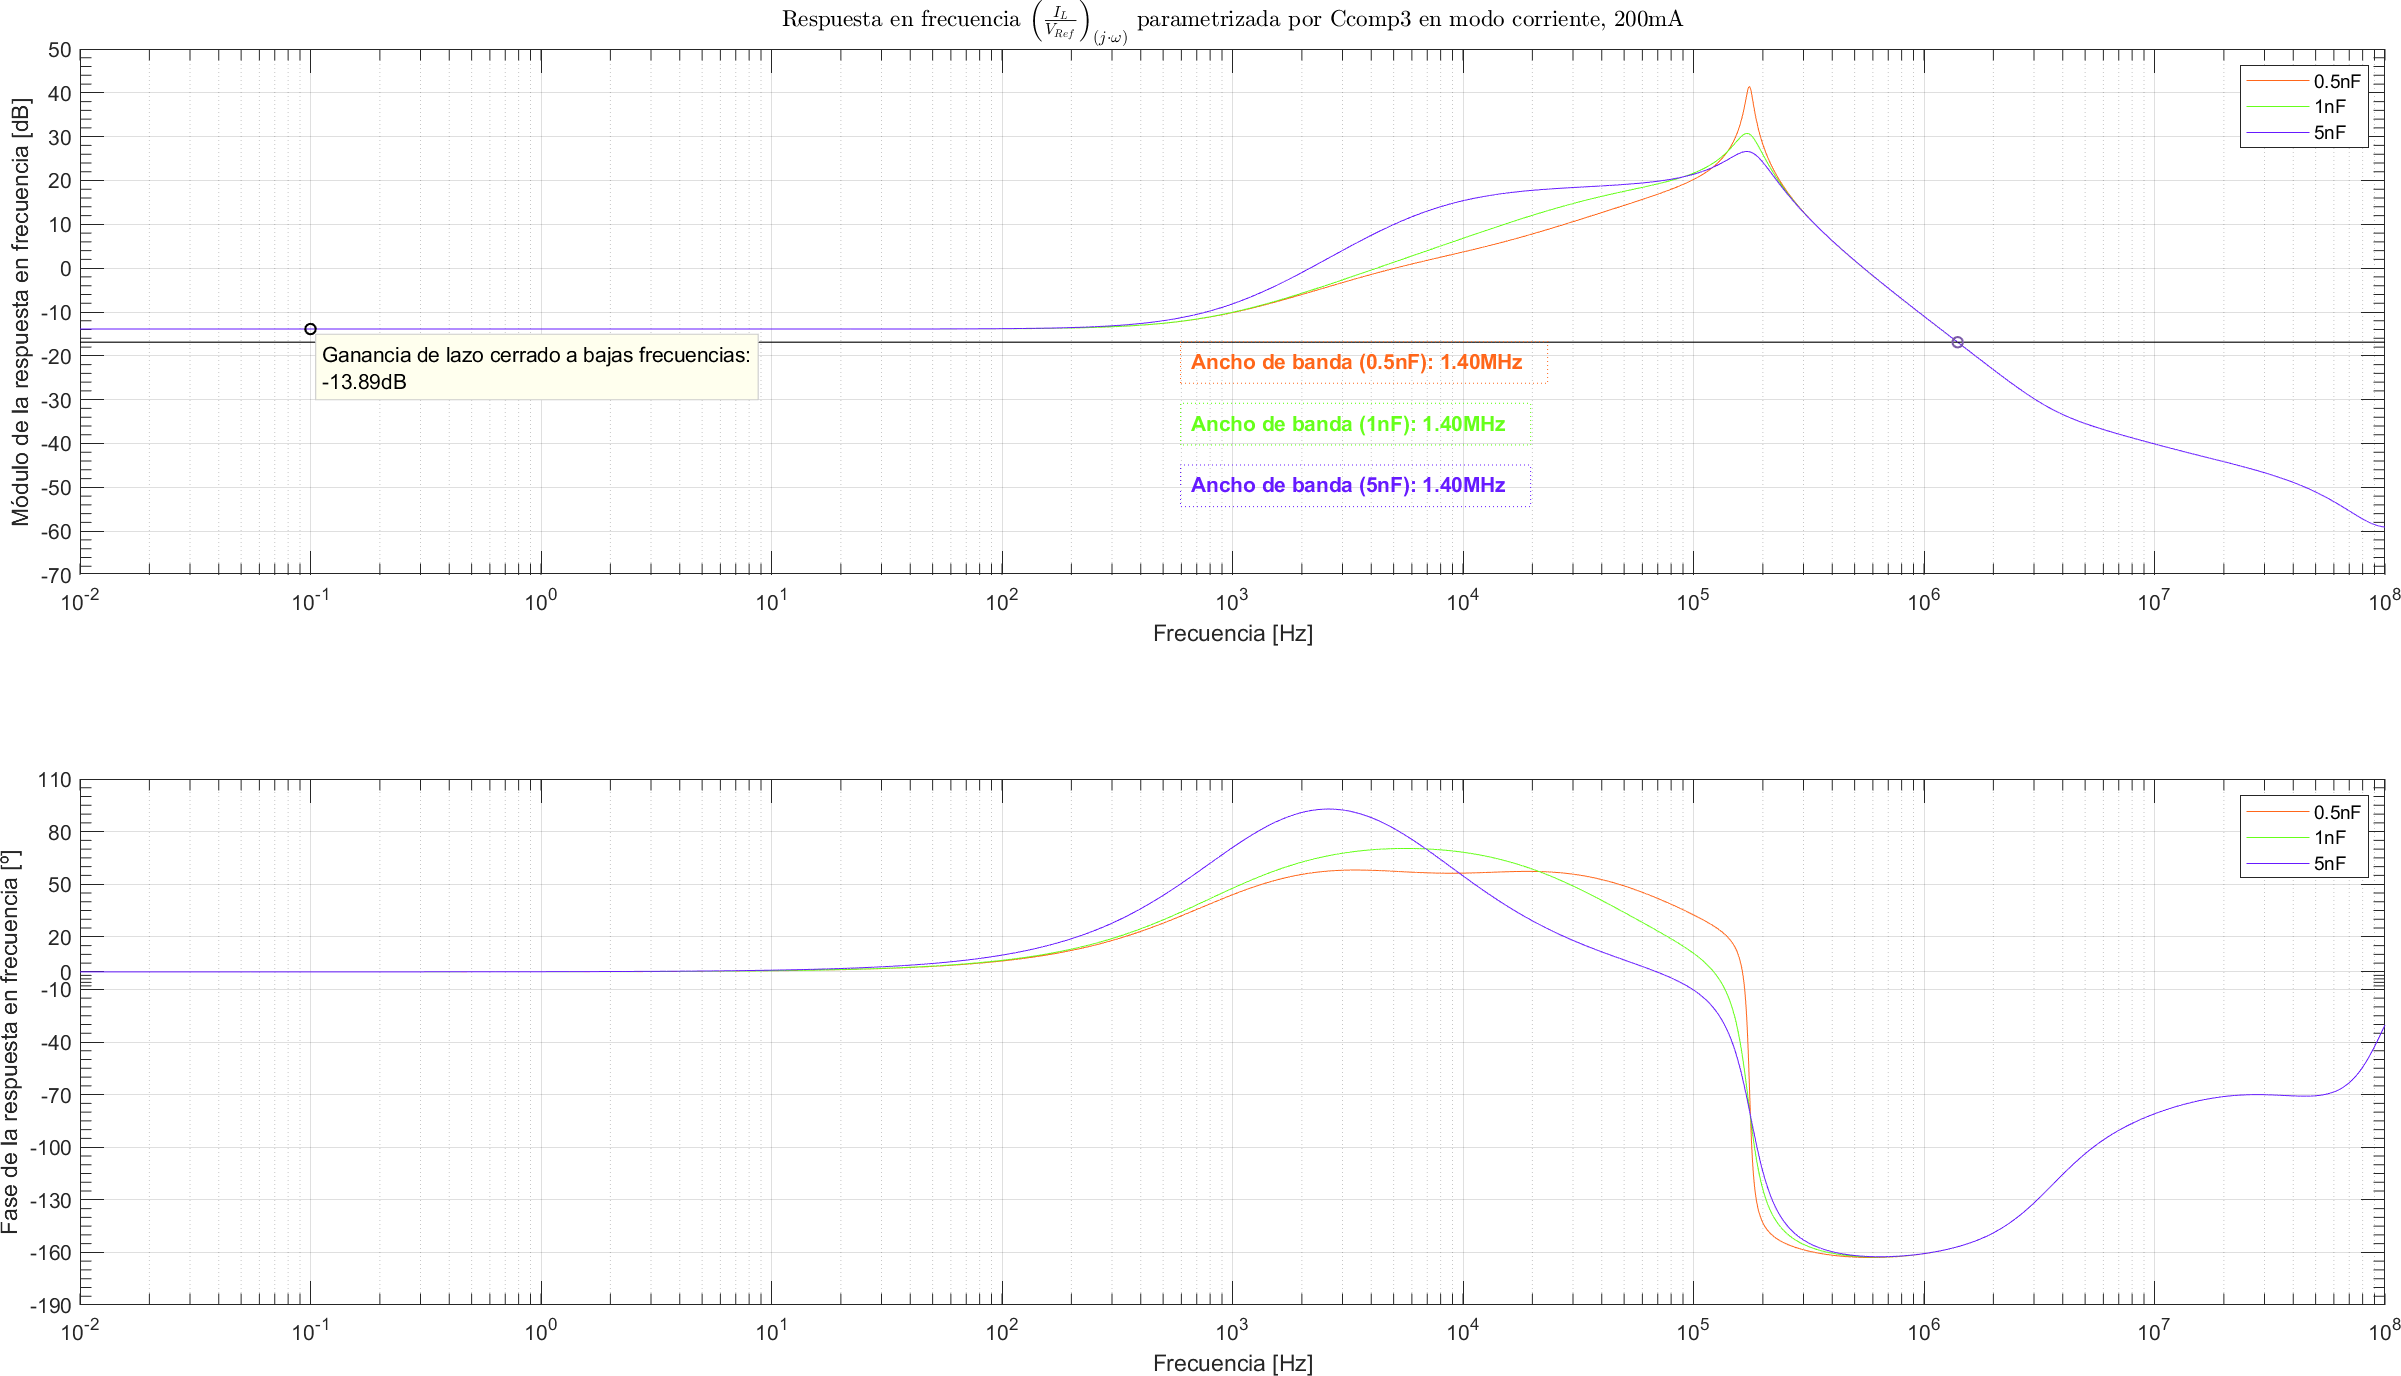
\includegraphics[width=1.1 \textwidth, angle=90]{./img/plots/rf/power_supply_CCOMP3_RF_Modo4.png}
\caption{\label{fig:fig_power_supply_CCOMP3_RF_Modo4}\footnotesize{Respuesta en frecuencia en modo corriente, $I_{out} = 200 \si[per-mode=symbol]{\milli\ampere}$, en función de la frecuencia parametrizada por $C_{comp_{3}}$.}}
\end{center}
\end{figure}

\clearpage

\begin{figure}[H] %htb
\begin{center}
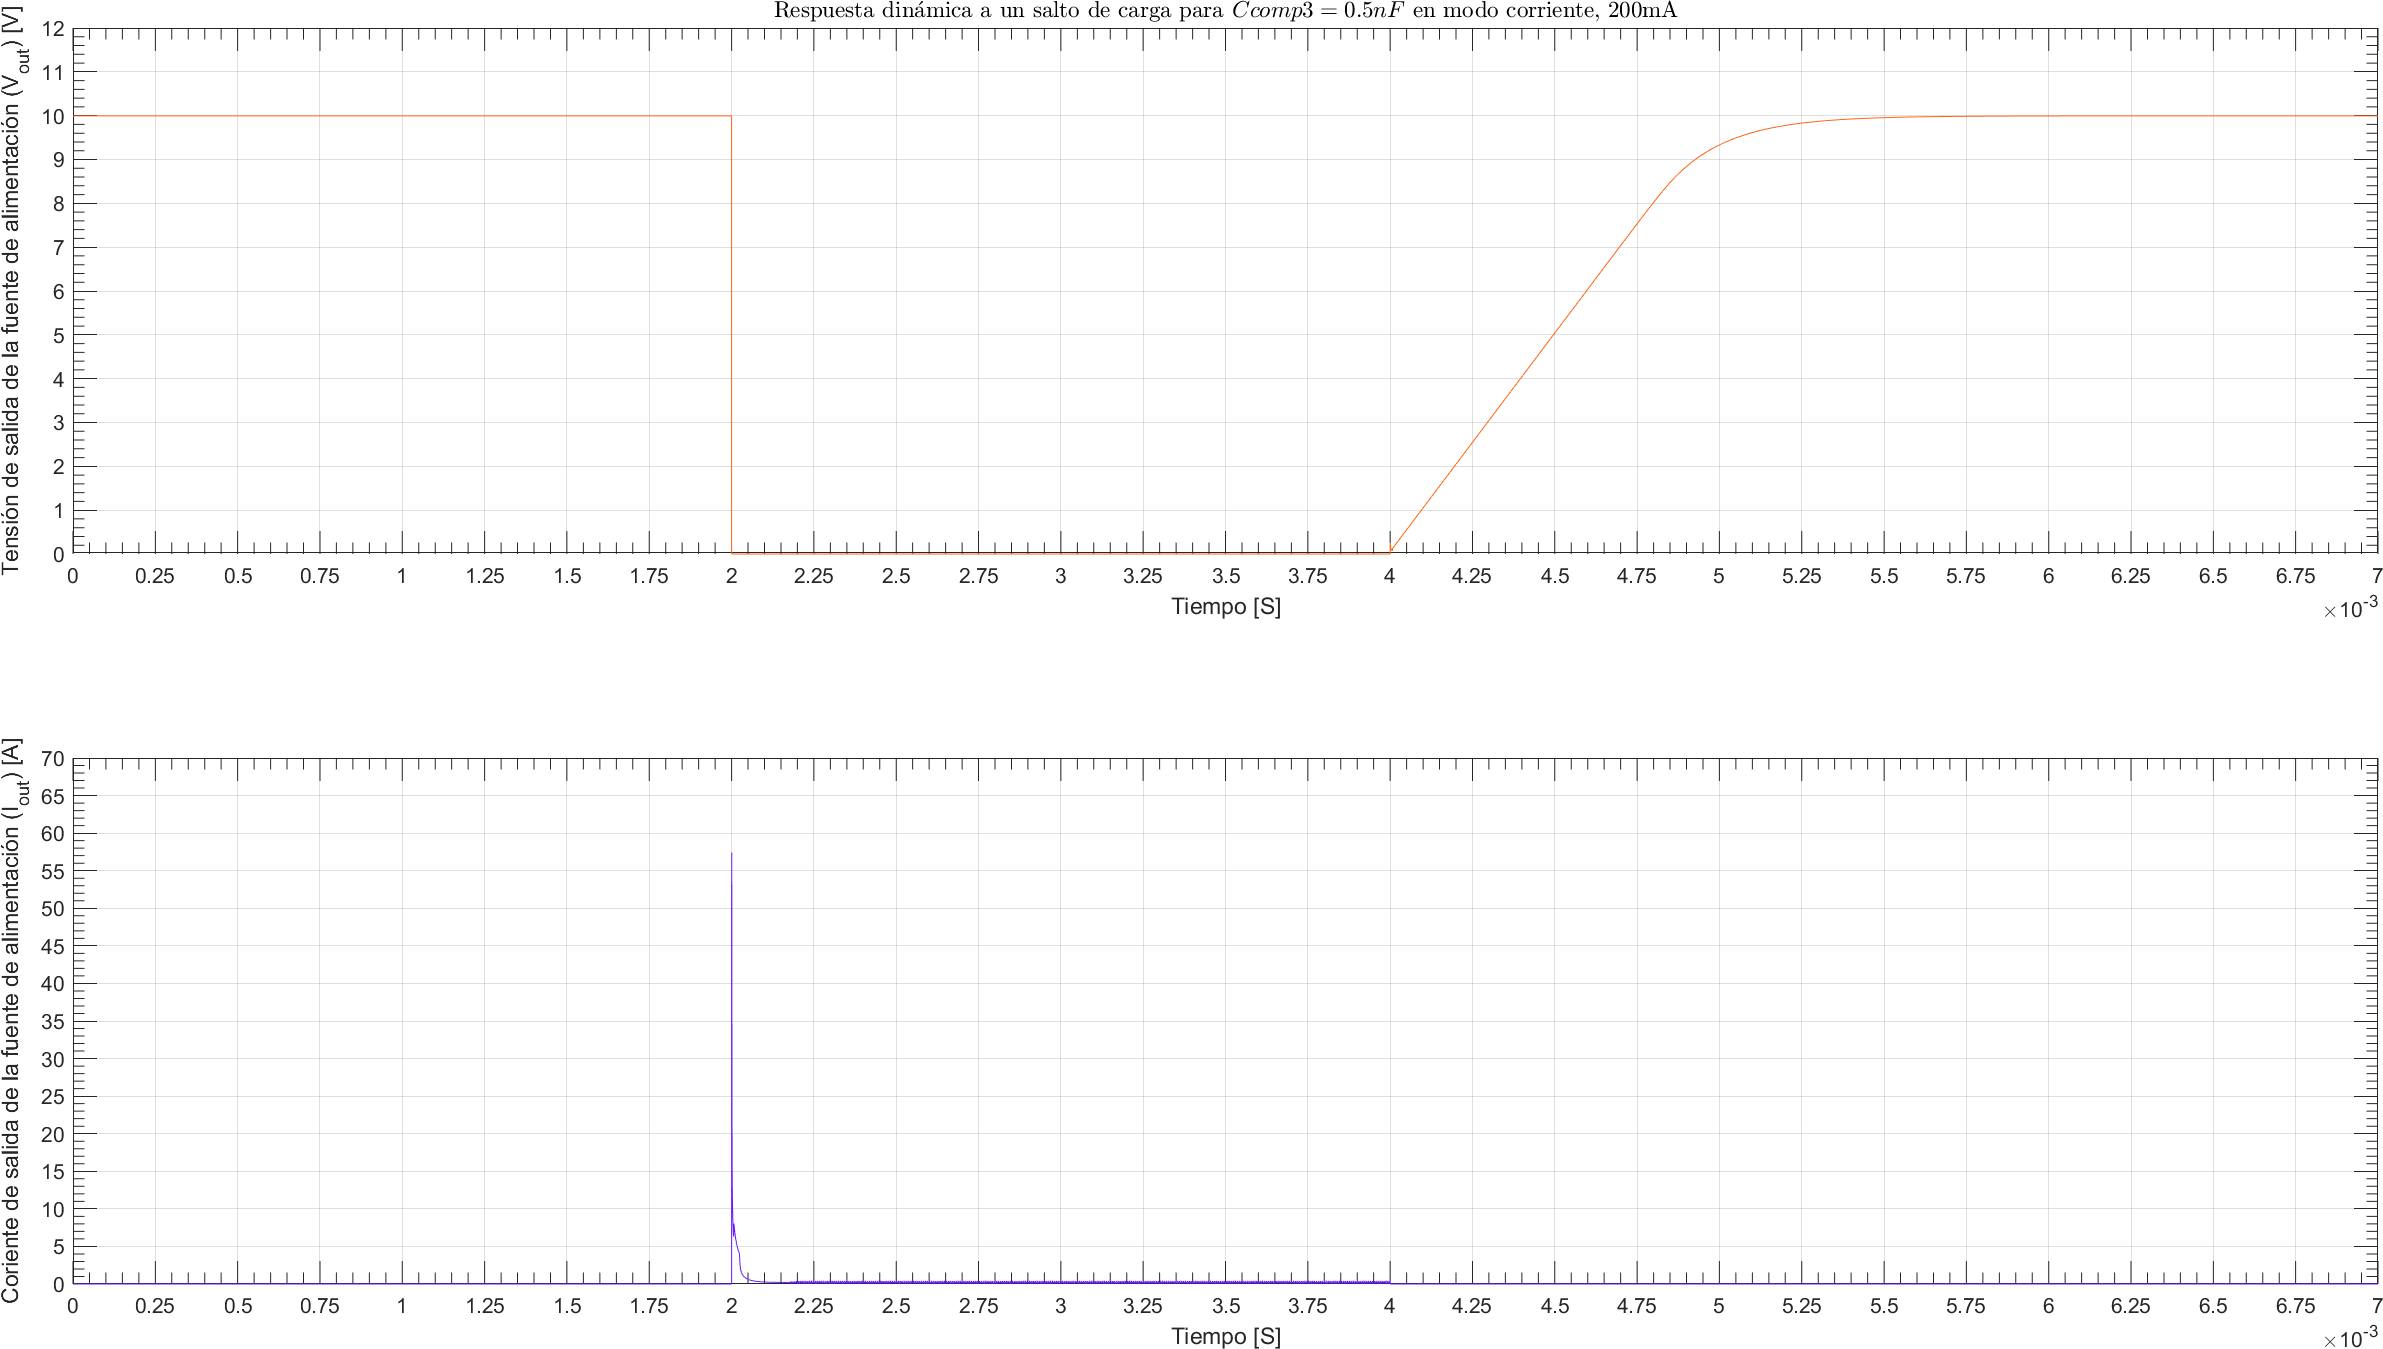
\includegraphics[width=1.1 \textwidth, angle=90]{./img/plots/dynamic/power_supply_CCOMP3_0_5n_STEP_Modo4.png}
\caption{\label{fig:fig_power_supply_CCOMP3_STEP_0_5n_Modo4}\footnotesize{Respuesta dinámica en modo corriente, $I_{out} = 200 \si[per-mode=symbol]{\milli\ampere}$, para $C_{comp_{3}} = 0.5 \si[per-mode=symbol]{\nano\farad} $.}}
\end{center}
\end{figure}

\clearpage

\begin{figure}[H] %htb
\begin{center}
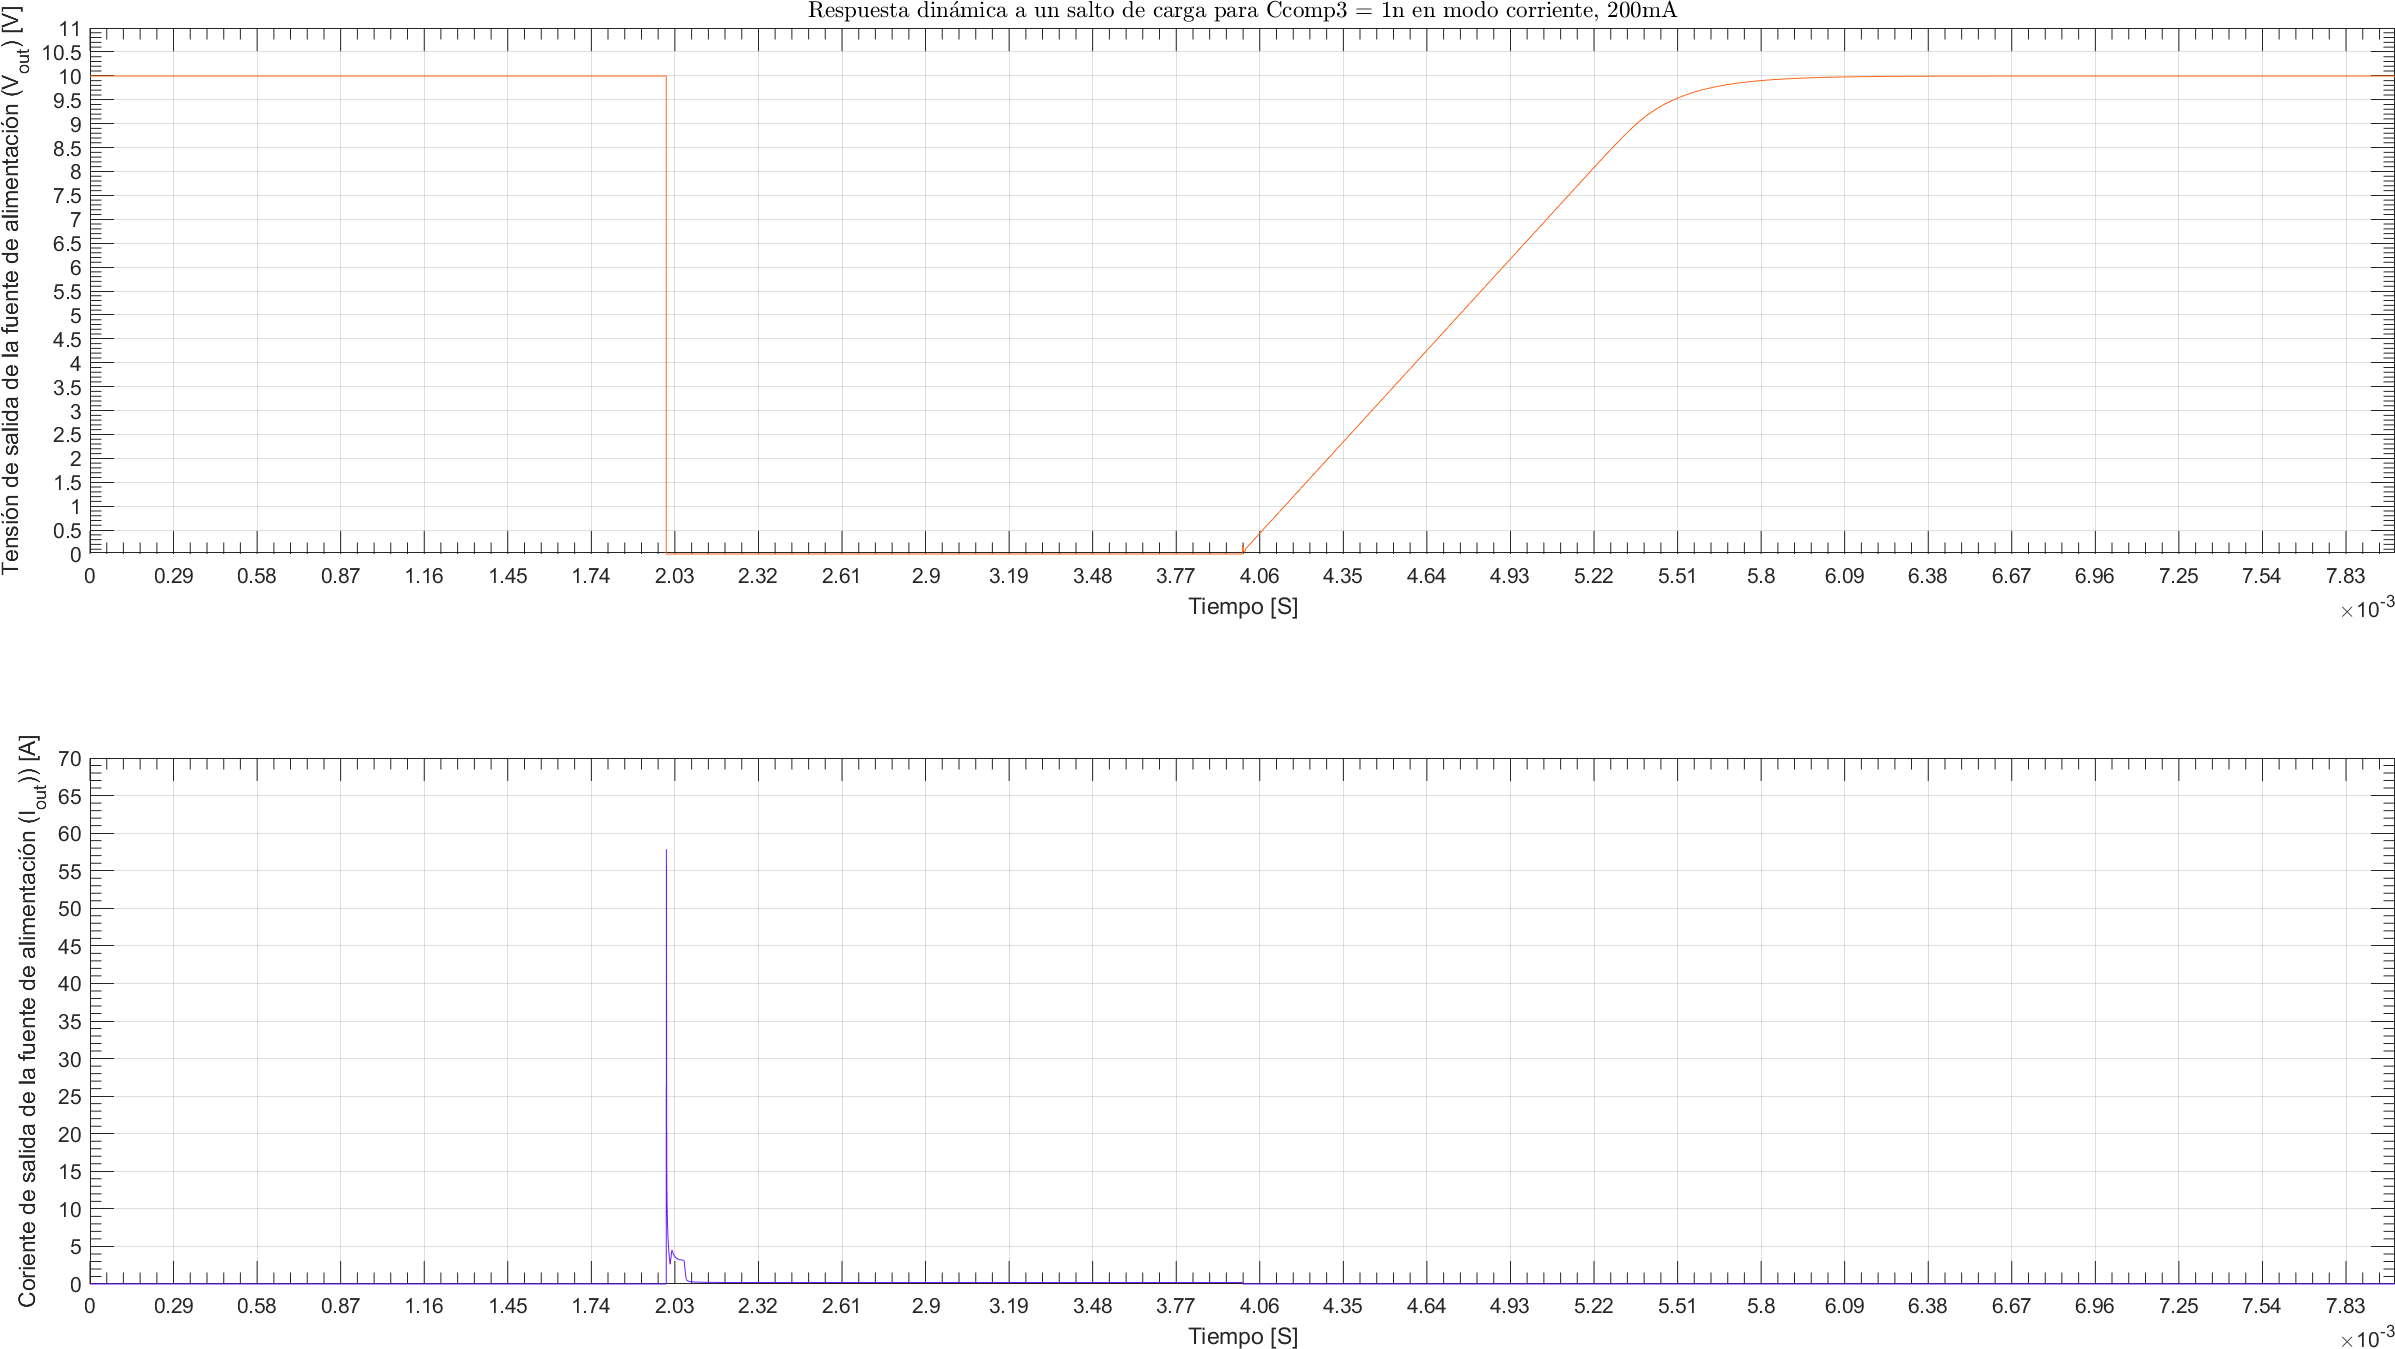
\includegraphics[width=1.1 \textwidth, angle=90]{./img/plots/dynamic/power_supply_CCOMP3_1n_STEP_Modo4.png}
\caption{\label{fig:fig_power_supply_CCOMP3_STEP_1n_Modo4}\footnotesize{Respuesta dinámica en modo corriente, $I_{out} = 200 \si[per-mode=symbol]{\milli\ampere}$, para $C_{comp_{3}} = 1 \si[per-mode=symbol]{\nano\farad} $.}}
\end{center}
\end{figure}

\clearpage

\begin{figure}[H] %htb
\begin{center}
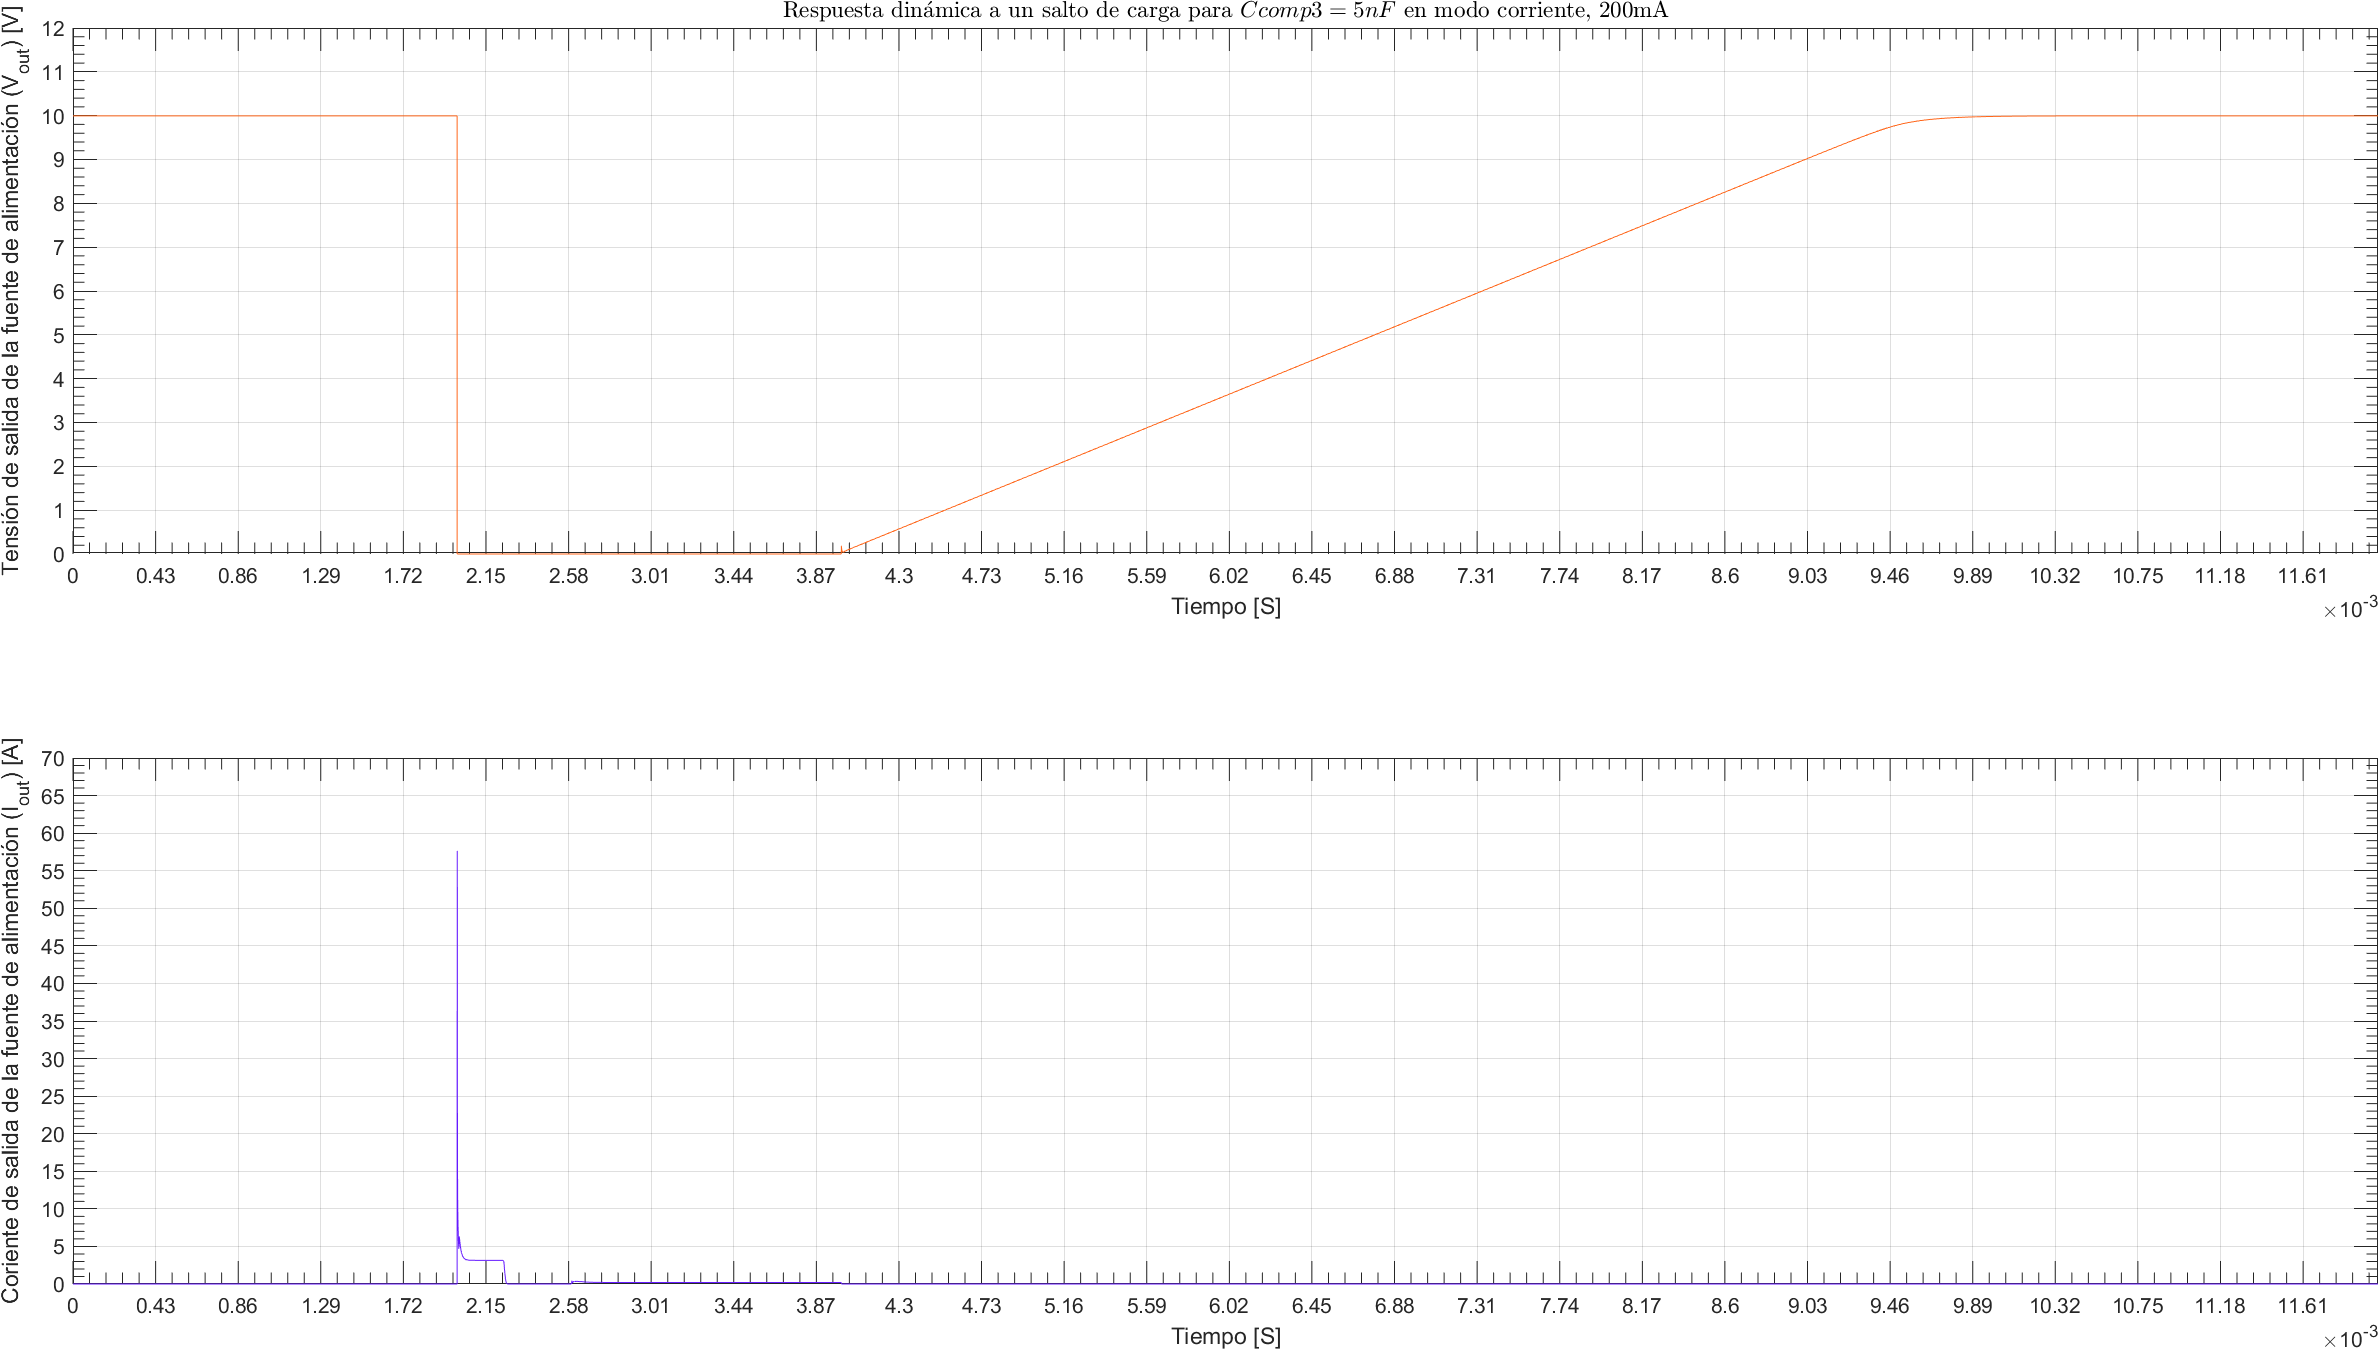
\includegraphics[width=1.1 \textwidth, angle=90]{./img/plots/dynamic/power_supply_CCOMP3_5n_STEP_Modo4.png}
\caption{\label{fig:fig_power_supply_CCOMP3_STEP_5n_Modo4}\footnotesize{Respuesta dinámica en modo corriente, $I_{out} = 200 \si[per-mode=symbol]{\milli\ampere}$, para $C_{comp_{3}} = 5 \si[per-mode=symbol]{\nano\farad} $.}}
\end{center}
\end{figure}

\clearpage







\clearpage
%\\\\\\\\\\\\\\\\\\\\\\\\\\\


%\\\\\\\\\\\\\\\\\\\\\\\\\\\
\subsection{Red de compensación de $C_{comp_{4}}/R_{comp_{4}}$}

La red que contiene a $\bm{C_{comp3}}$ actúa solo para el lazo de corriente, por lo que se analiza solo este modo.


\subsubsection{Análisis para $C_{comp_{4}}$ en modo corriente, $I_{out} = 200 \si[per-mode=symbol]{\milli\ampere}$, $R_{L} = 0 \si[per-mode=symbol]{\ohm}$}
% CCOMP4 MODO 4.

\clearpage

\begin{figure}[H] %htb
\begin{center}
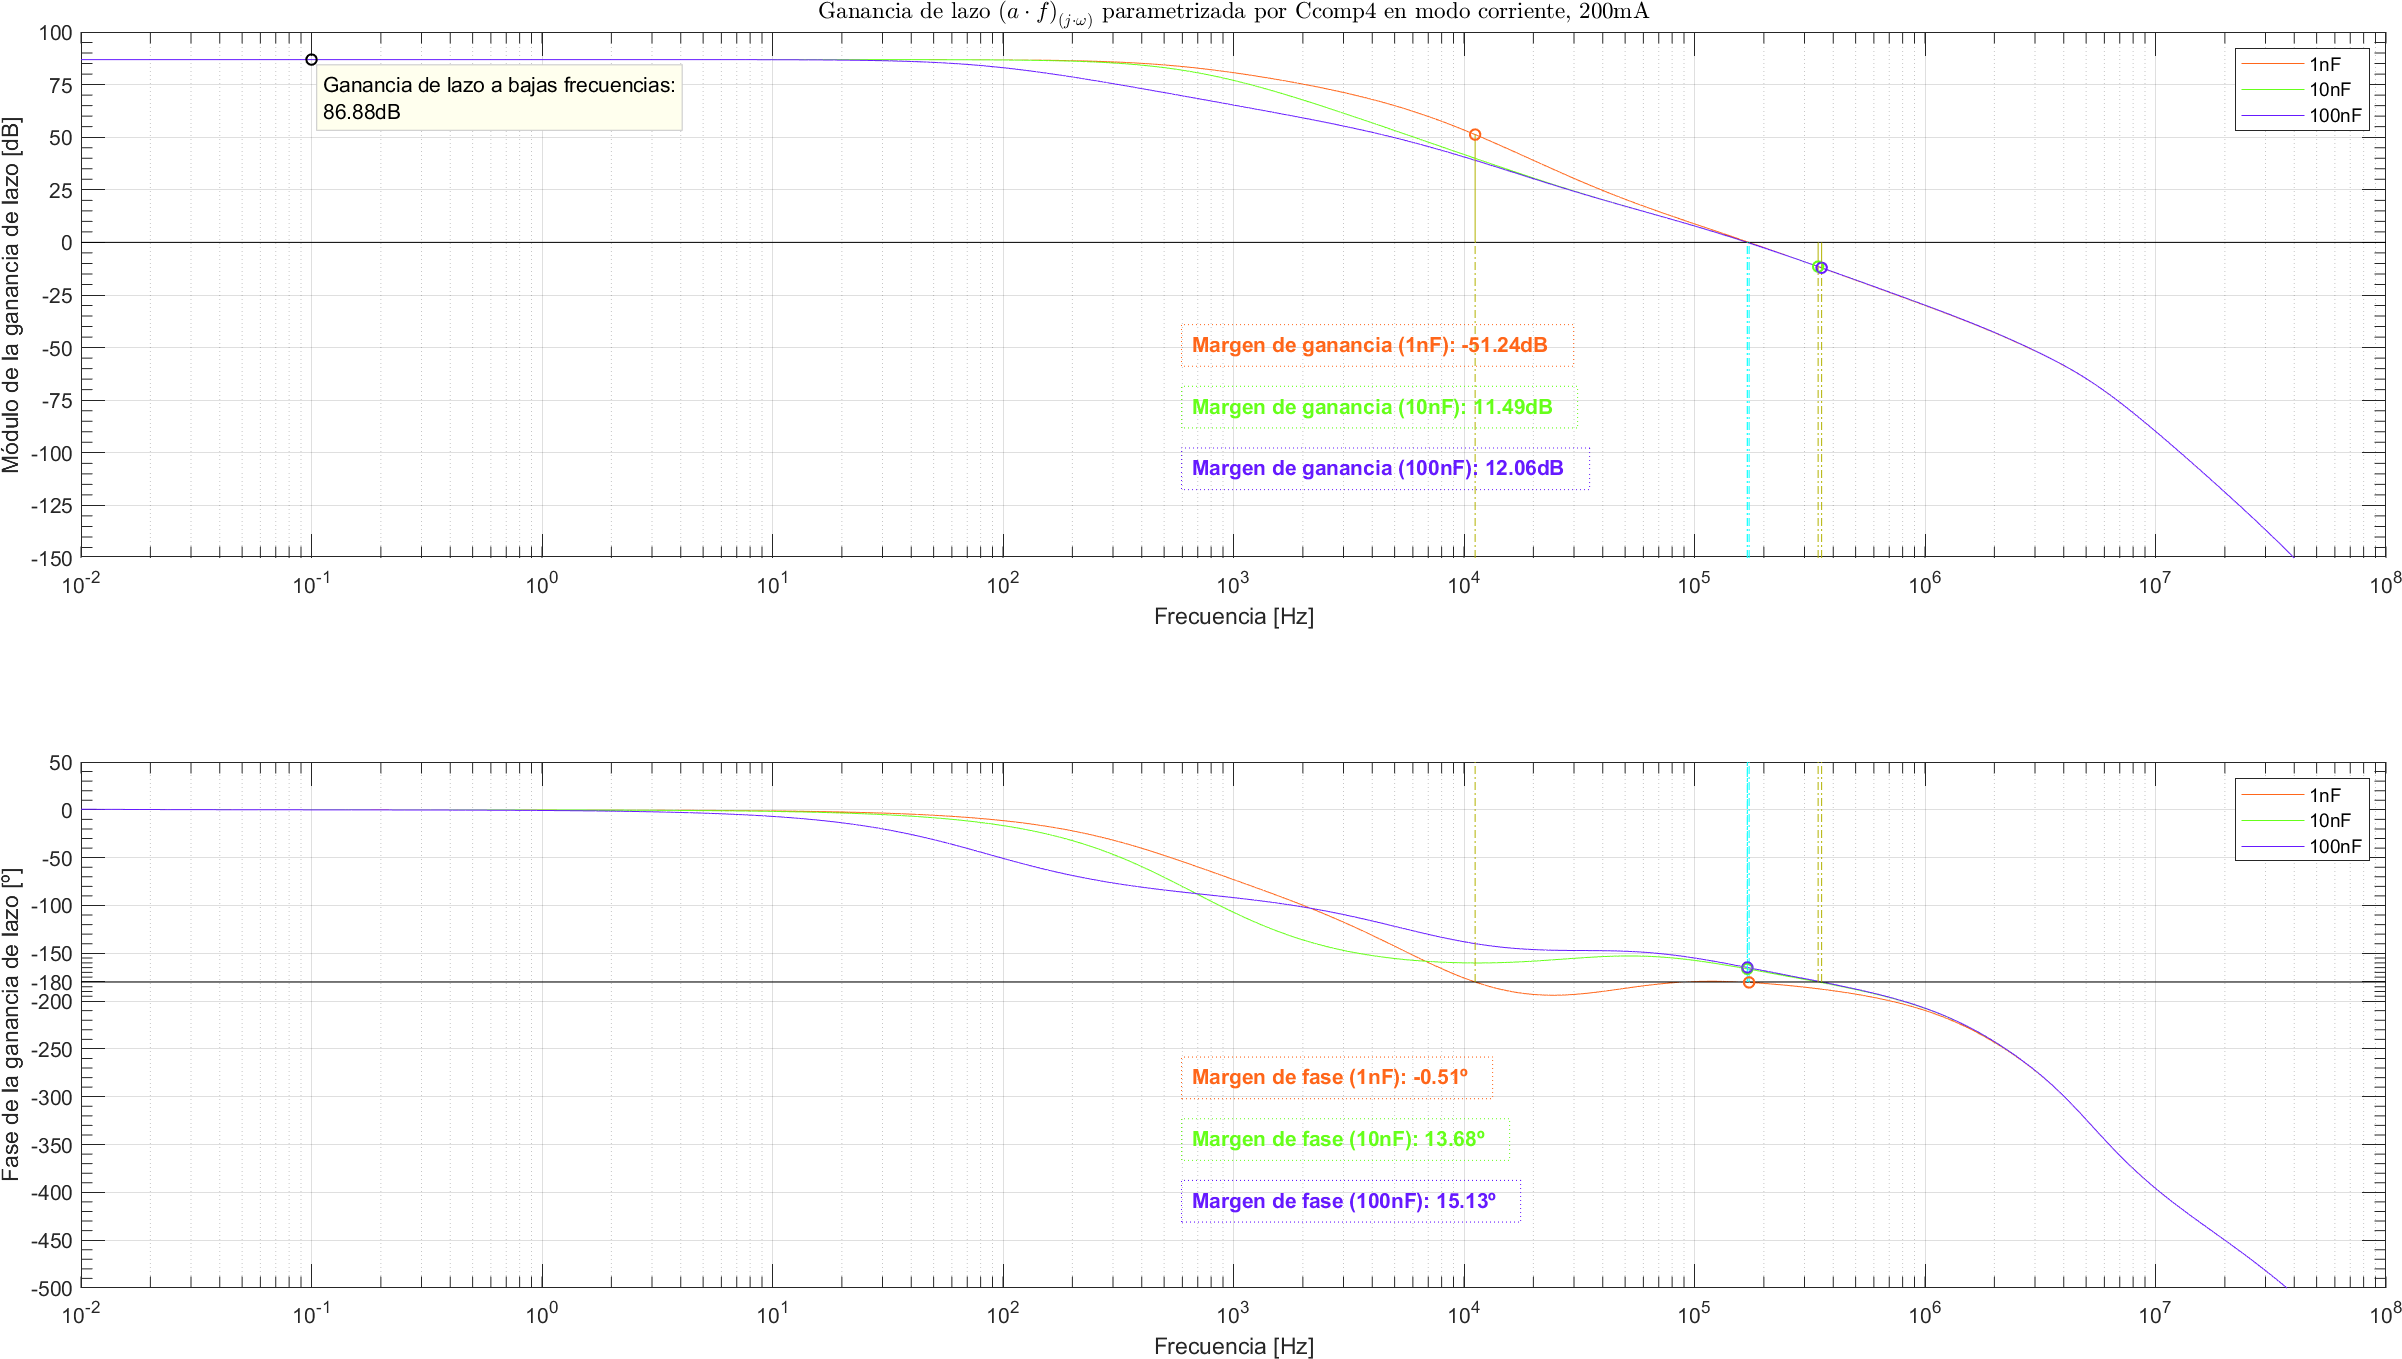
\includegraphics[width=1.1 \textwidth, angle=90]{./img/plots/loop/power_supply_CCOMP4_LOOP_Modo4.png}
\caption{\label{fig:fig_power_supply_CCOMP4_LOOP_Modo4}\footnotesize{Ganancia de lazo en modo corriente, $I_{out} = 200 \si[per-mode=symbol]{\milli\ampere}$, en función de la frecuencia parametrizada por $C_{comp_{4}}$.}}
\end{center}
\end{figure}


\clearpage

\begin{figure}[H] %htb
\begin{center}
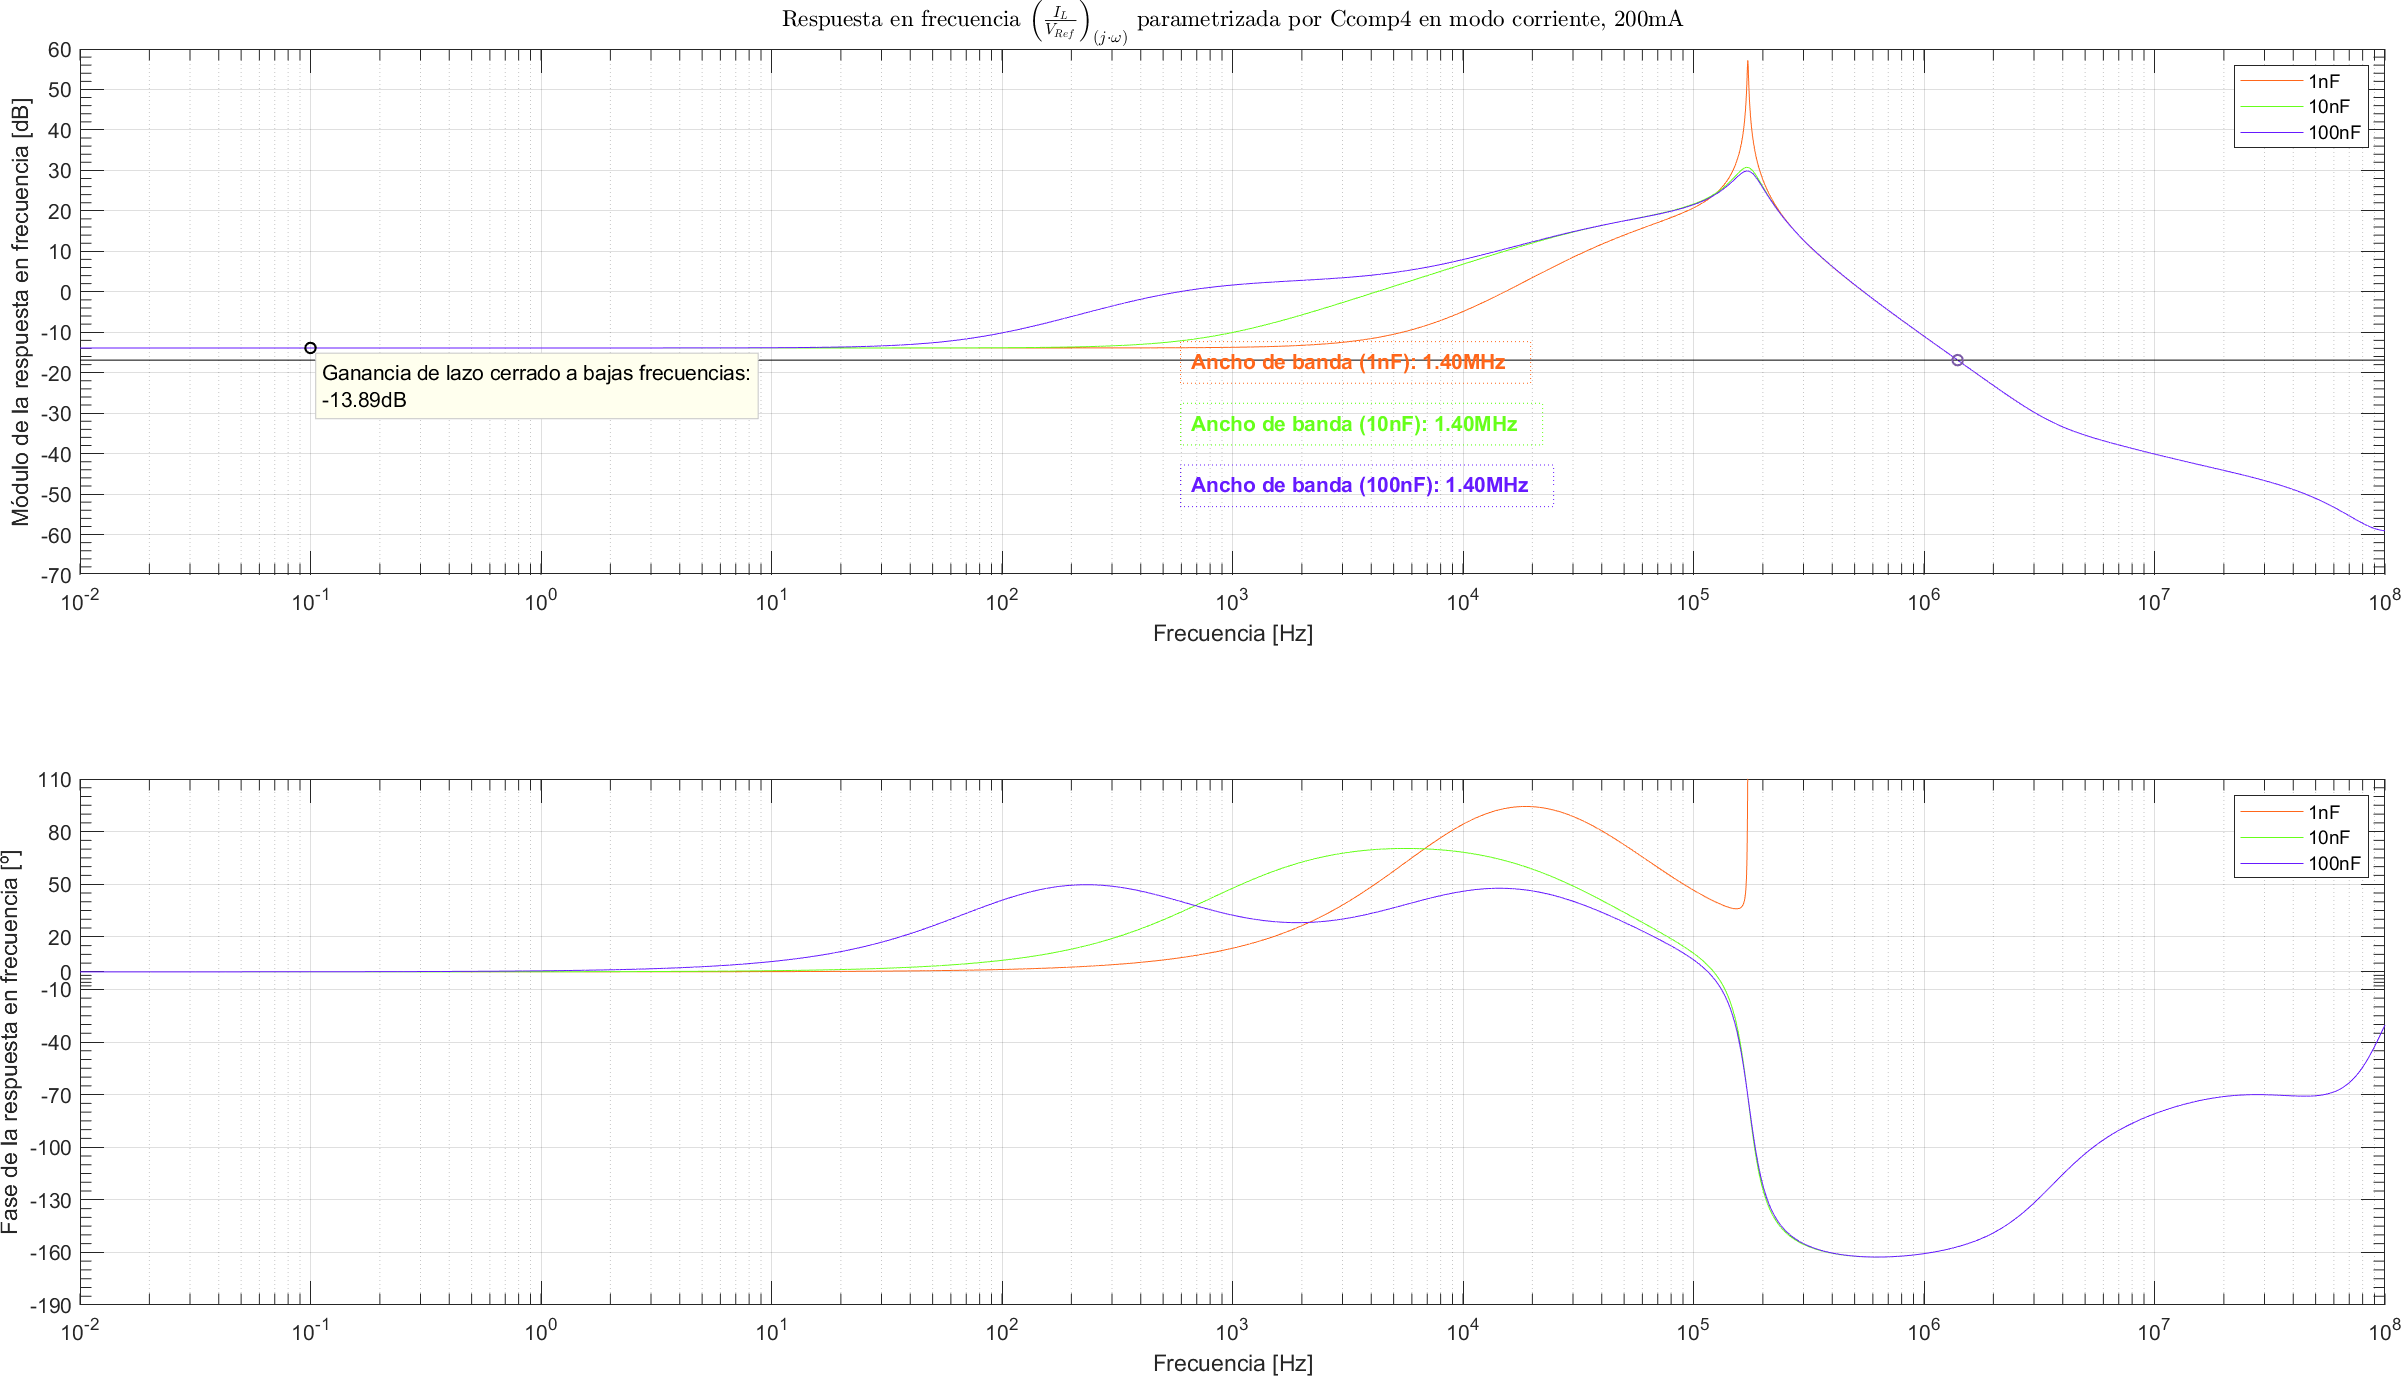
\includegraphics[width=1.1 \textwidth, angle=90]{./img/plots/rf/power_supply_CCOMP4_RF_Modo4.png}
\caption{\label{fig:fig_power_supply_CCOMP4_RF_Modo4}\footnotesize{Respuesta en frecuencia en modo corriente, $I_{out} = 200 \si[per-mode=symbol]{\milli\ampere}$, en función de la frecuencia parametrizada por $C_{comp_{4}}$.}}
\end{center}
\end{figure}

\clearpage

\begin{figure}[H] %htb
\begin{center}
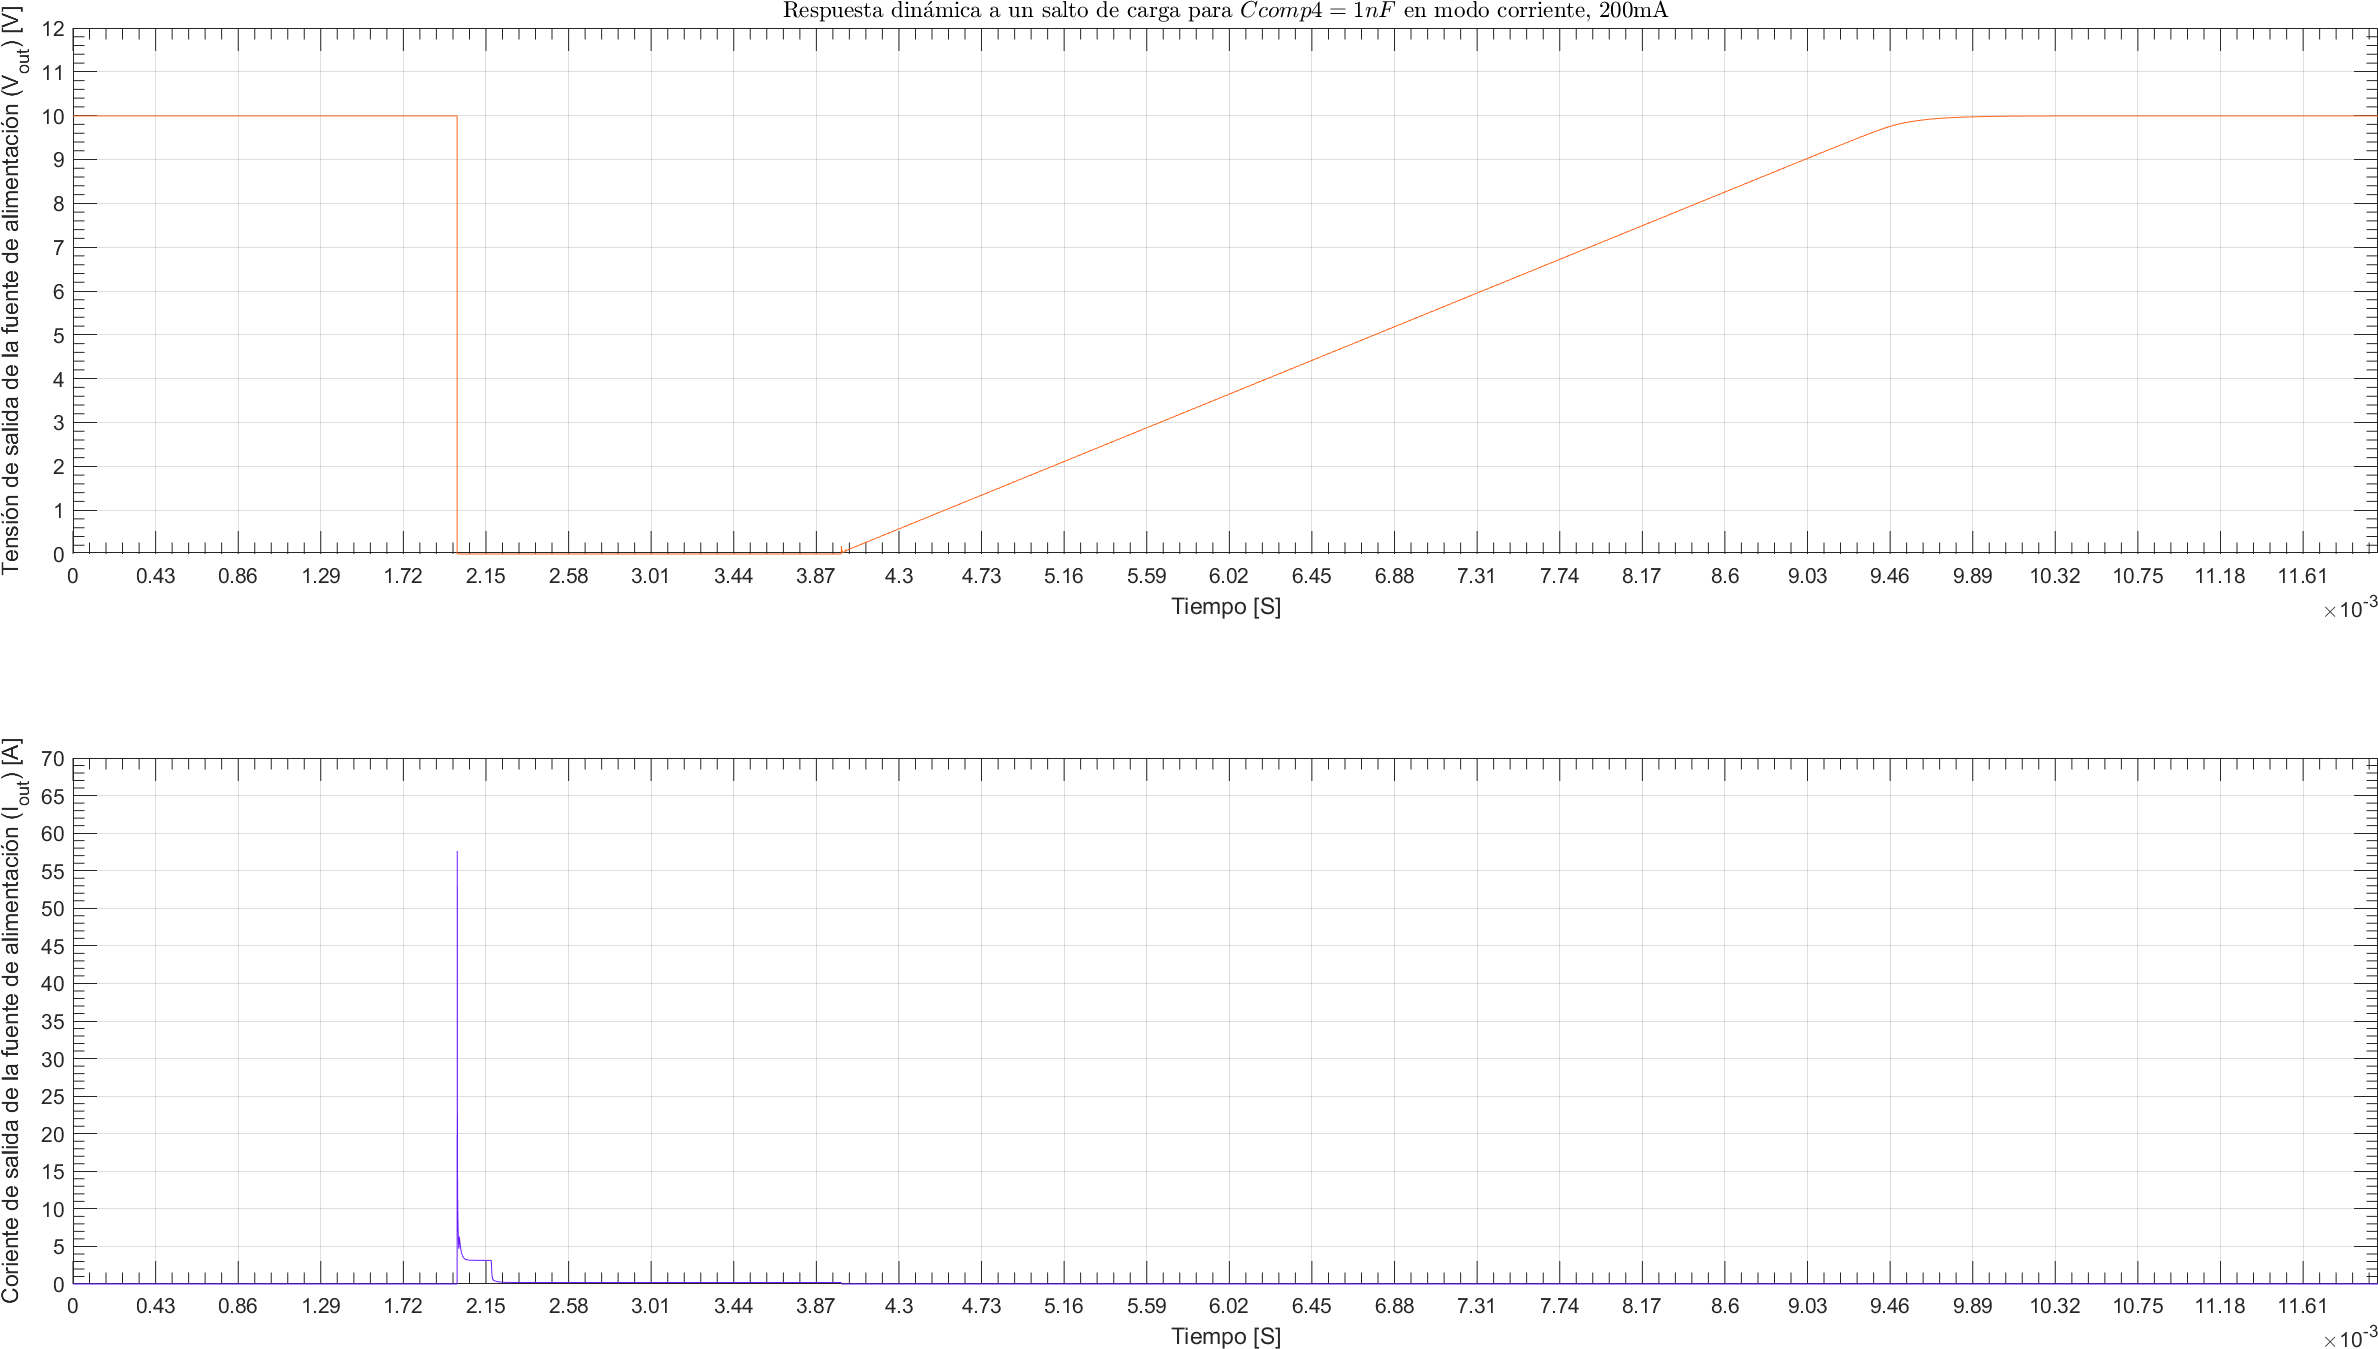
\includegraphics[width=1.1 \textwidth, angle=90]{./img/plots/dynamic/power_supply_CCOMP4_1n_STEP_Modo4.png}
\caption{\label{fig:fig_power_supply_CCOMP4_STEP_1n_Modo4}\footnotesize{Respuesta dinámica en modo corriente, $I_{out} = 200 \si[per-mode=symbol]{\milli\ampere}$, para $C_{comp_{4}} = 1 \si[per-mode=symbol]{\nano\farad} $.}}
\end{center}
\end{figure}

\clearpage

\begin{figure}[H] %htb
\begin{center}
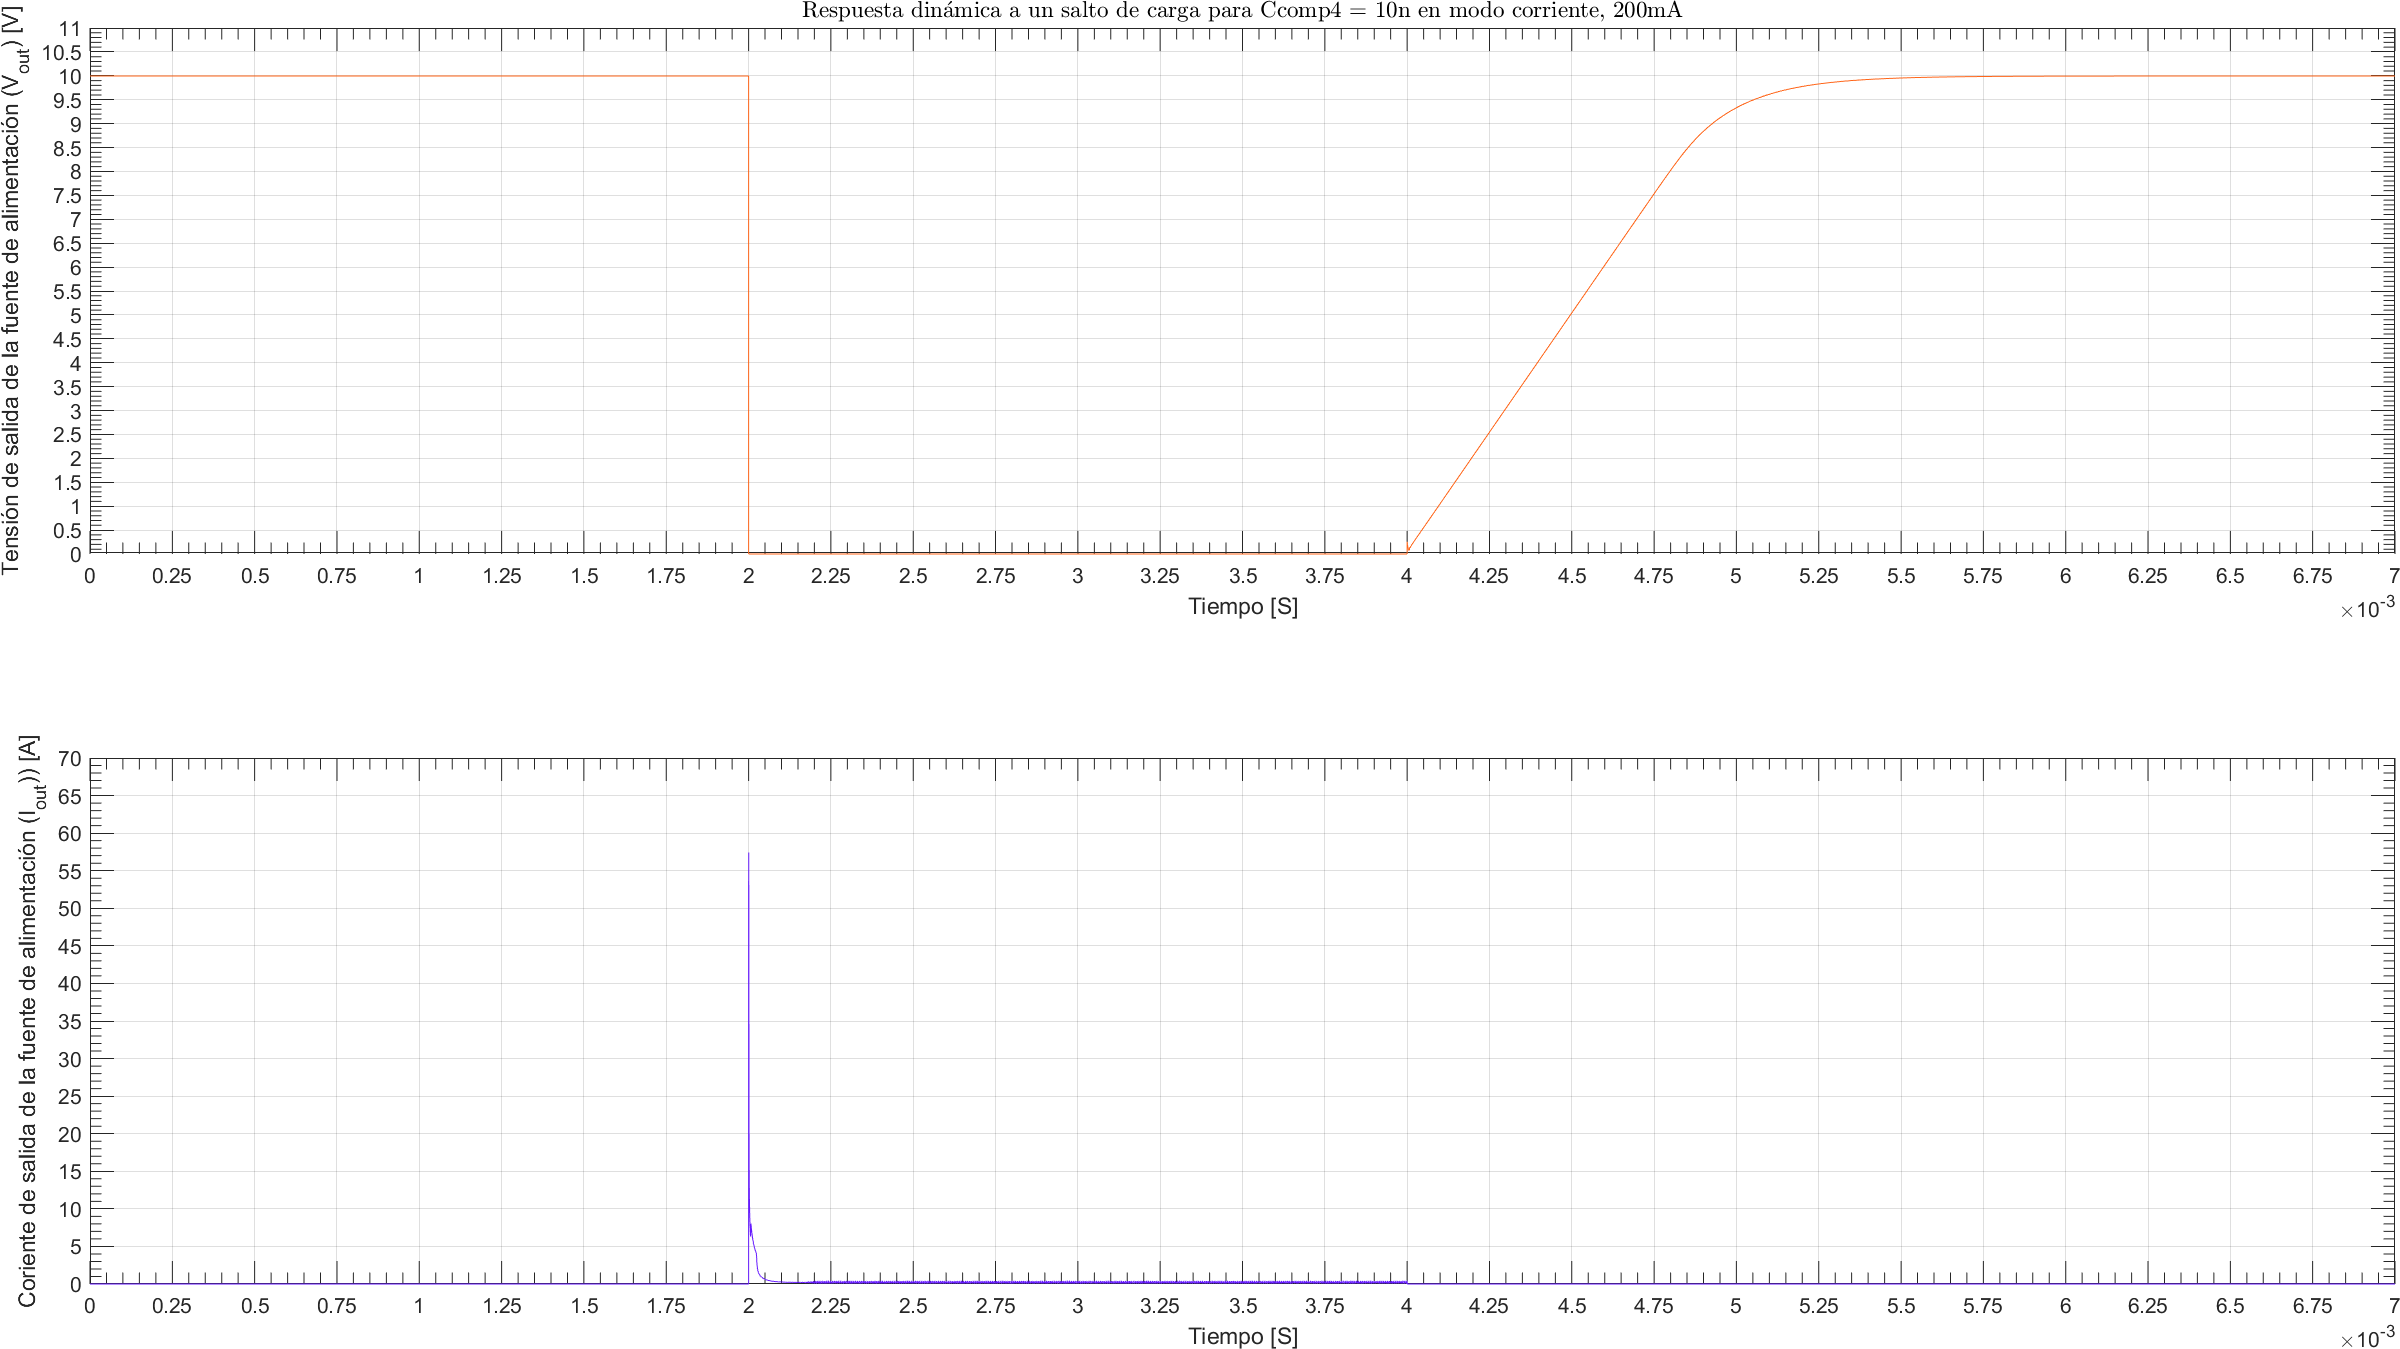
\includegraphics[width=1.1 \textwidth, angle=90]{./img/plots/dynamic/power_supply_CCOMP4_10n_STEP_Modo4.png}
\caption{\label{fig:fig_power_supply_CCOMP4_STEP_10n_Modo4}\footnotesize{Respuesta dinámica en modo corriente, $I_{out} = 200 \si[per-mode=symbol]{\milli\ampere}$, para $C_{comp_{4}} = 10 \si[per-mode=symbol]{\nano\farad} $.}}
\end{center}
\end{figure}

\clearpage

\begin{figure}[H] %htb
\begin{center}
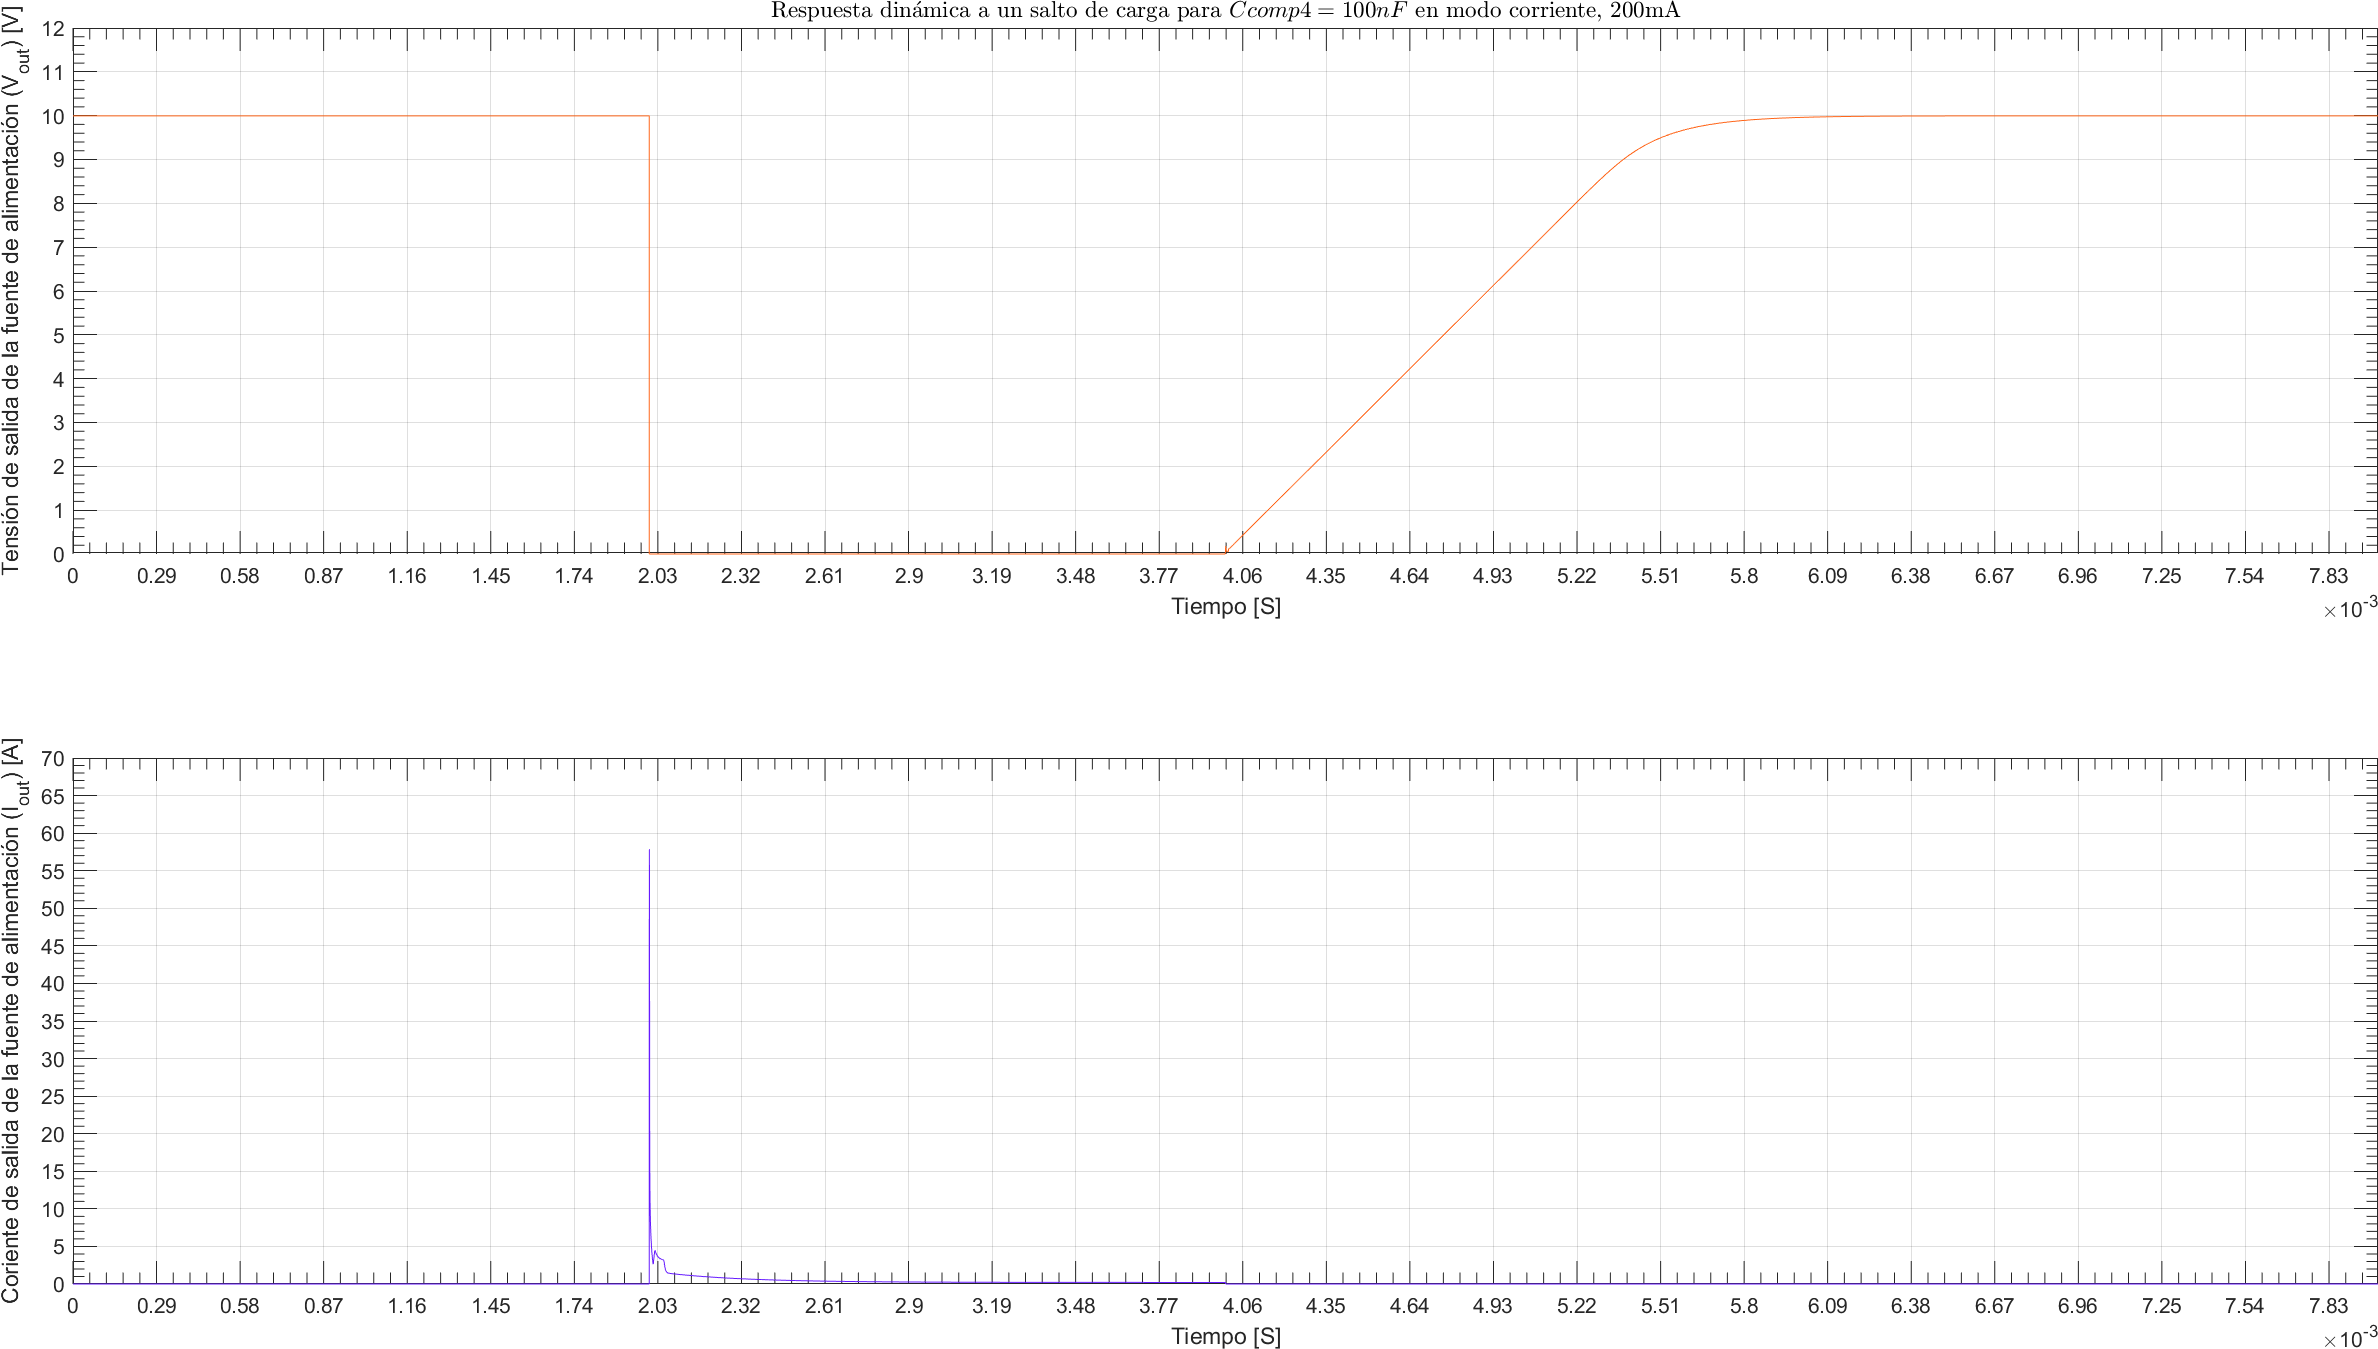
\includegraphics[width=1.1 \textwidth, angle=90]{./img/plots/dynamic/power_supply_CCOMP4_100n_STEP_Modo4.png}
\caption{\label{fig:fig_power_supply_CCOMP4_STEP_100n_Modo4}\footnotesize{Respuesta dinámica en modo corriente, $I_{out} = 200 \si[per-mode=symbol]{\milli\ampere}$, para $C_{comp_{4}} = 100 \si[per-mode=symbol]{\nano\farad} $.}}
\end{center}
\end{figure}

\clearpage






\subsubsection{Análisis para $R_{comp_{4}}$ en modo corriente, $I_{out} = 200 \si[per-mode=symbol]{\milli\ampere}$, $R_{L} = 0 \si[per-mode=symbol]{\ohm}$}
% CCOMP4 MODO 4.

\clearpage

\begin{figure}[H] %htb
\begin{center}
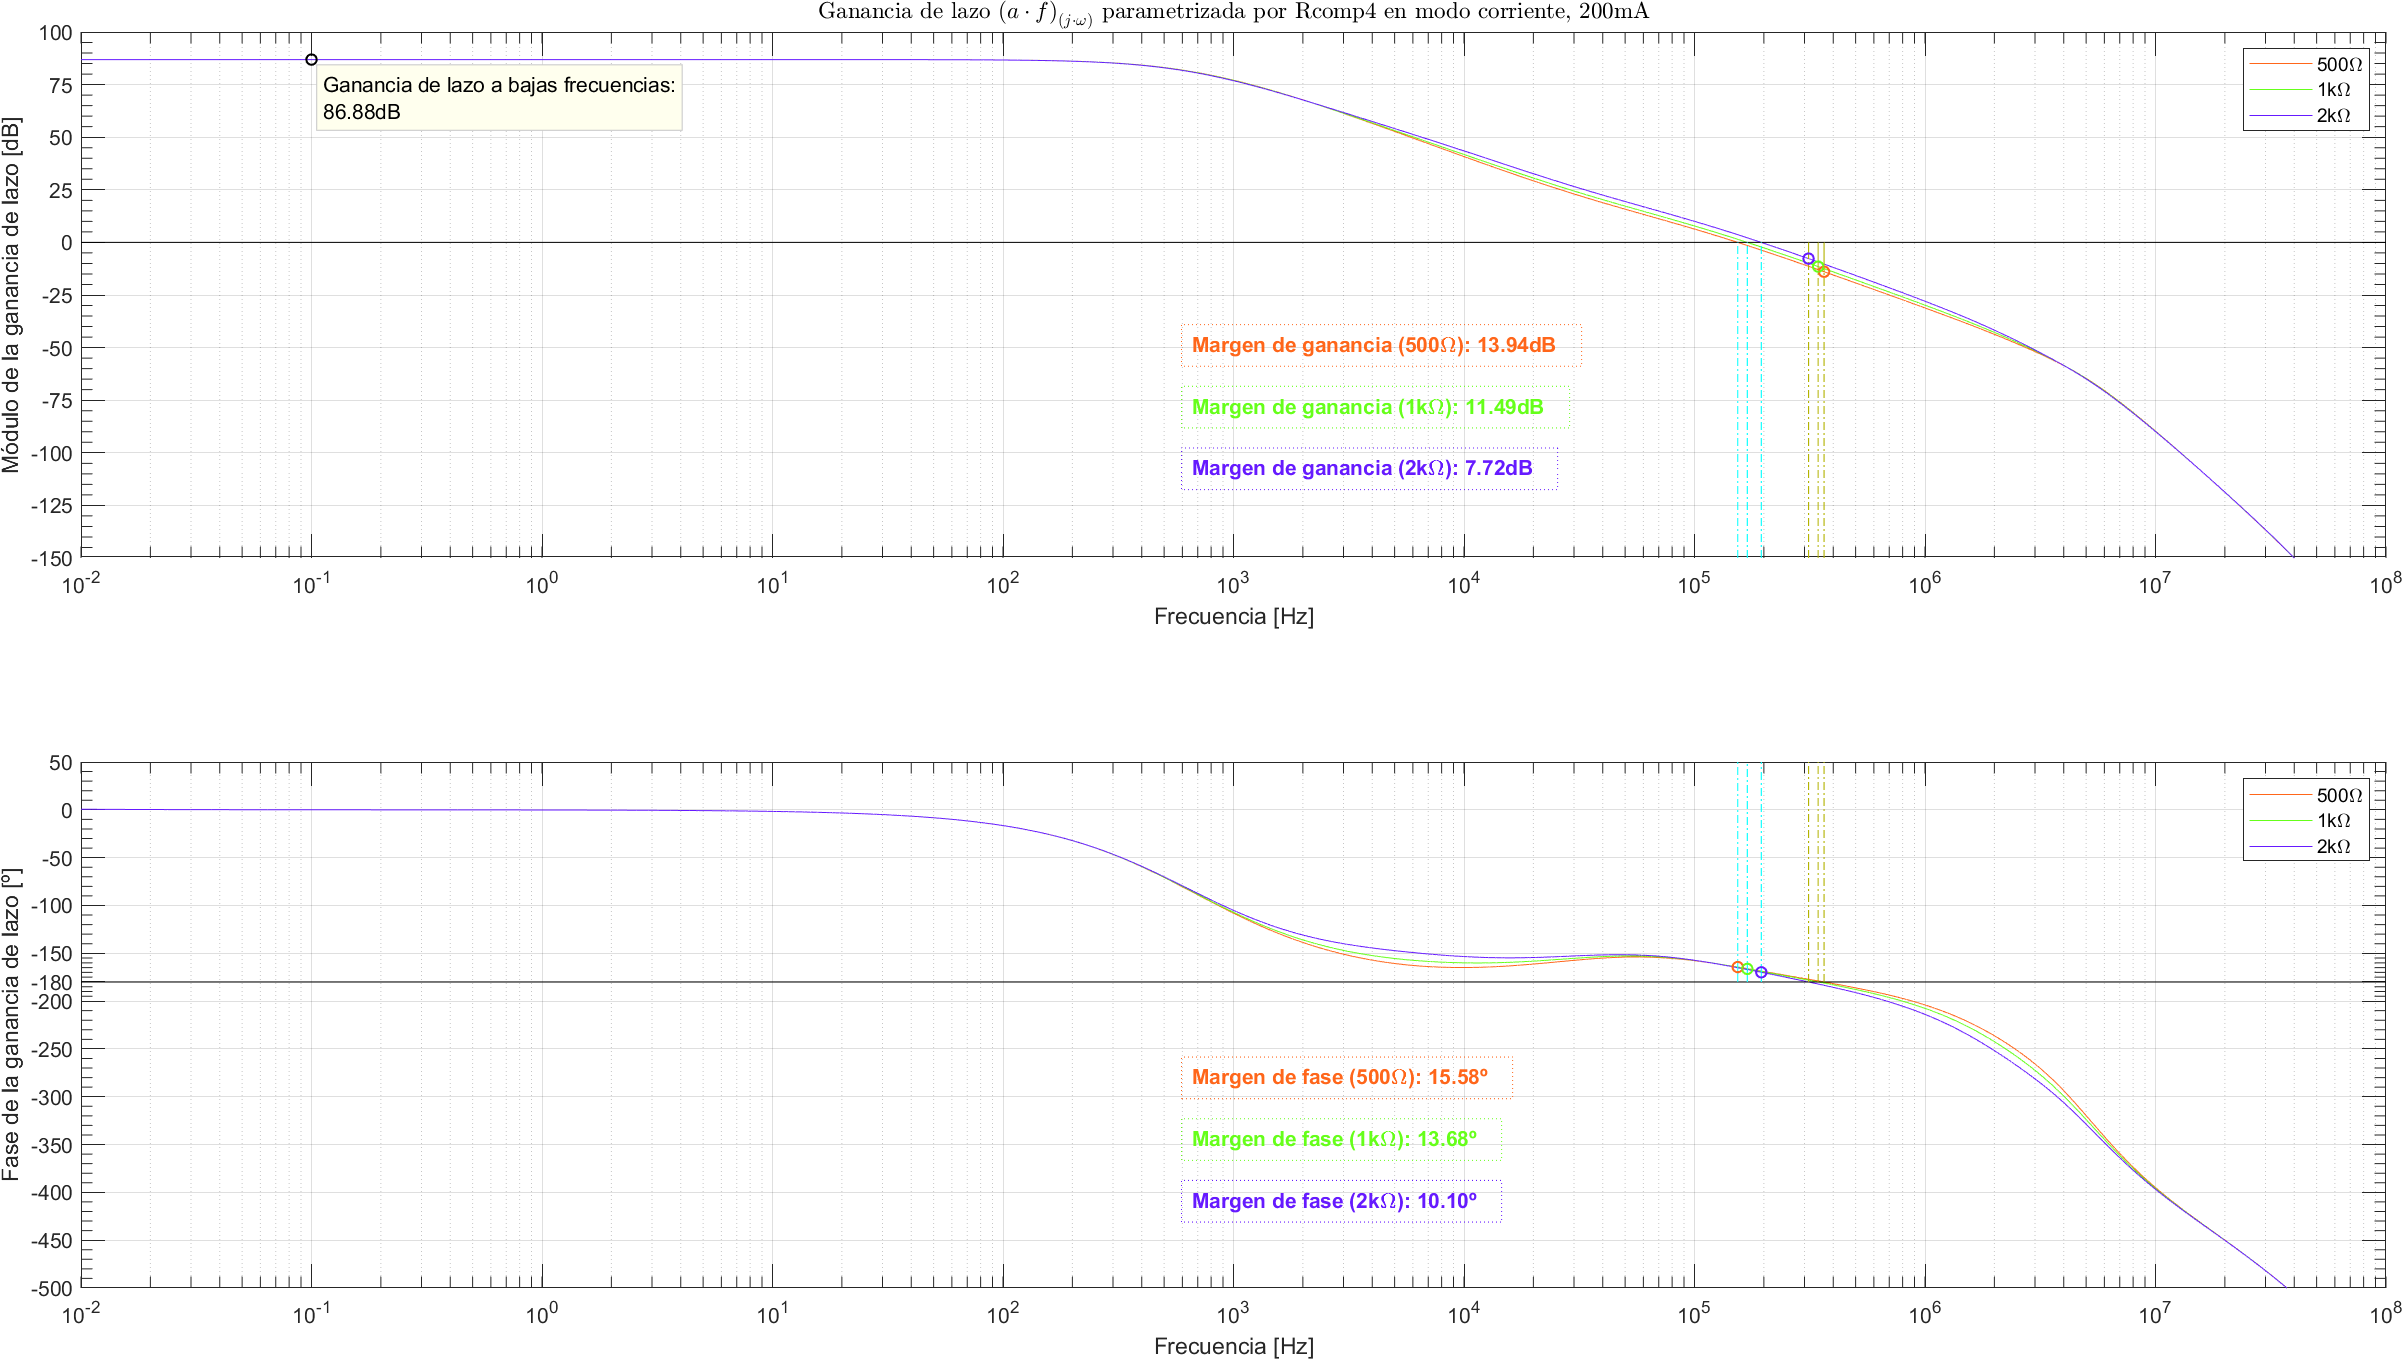
\includegraphics[width=1.1 \textwidth, angle=90]{./img/plots/loop/power_supply_RCOMP4_LOOP_Modo4.png}
\caption{\label{fig:fig_power_supply_RCOMP4_LOOP_Modo4}\footnotesize{Ganancia de lazo en modo corriente, $I_{out} = 200 \si[per-mode=symbol]{\milli\ampere}$, en función de la frecuencia parametrizada por $R_{comp_{4}}$.}}
\end{center}
\end{figure}


\clearpage

\begin{figure}[H] %htb
\begin{center}
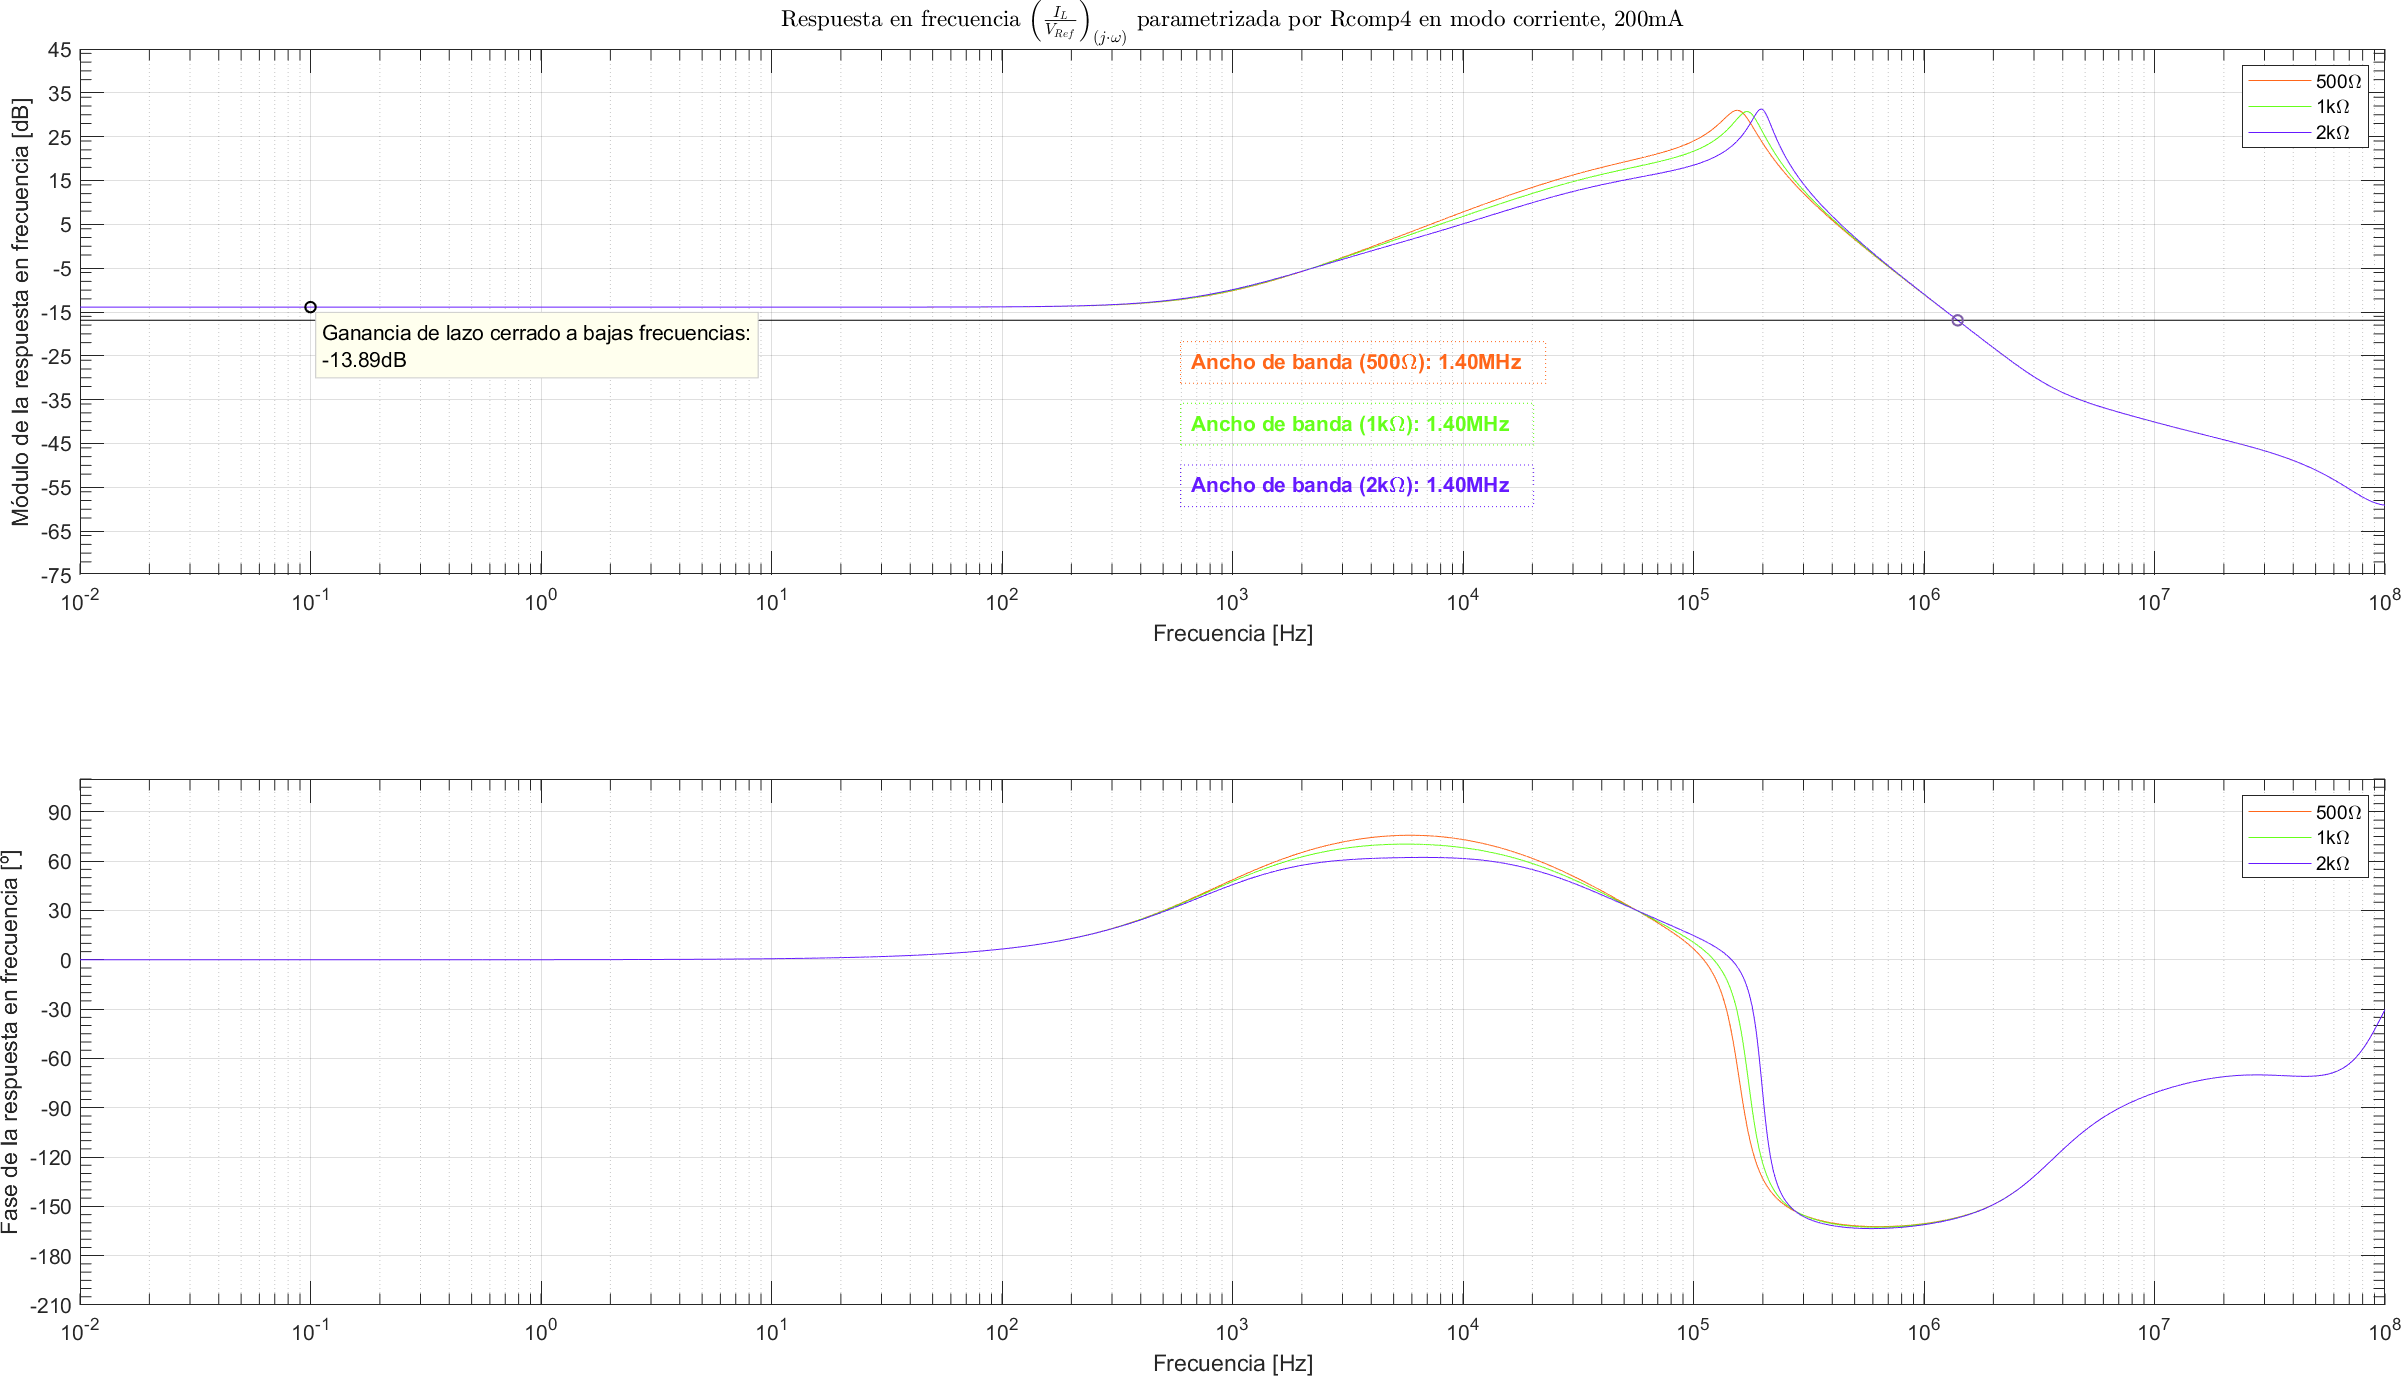
\includegraphics[width=1.1 \textwidth, angle=90]{./img/plots/rf/power_supply_RCOMP4_RF_Modo4.png}
\caption{\label{fig:fig_power_supply_RCOMP4_RF_Modo4}\footnotesize{Respuesta en frecuencia en modo corriente, $I_{out} = 200 \si[per-mode=symbol]{\milli\ampere}$, en función de la frecuencia parametrizada por $R_{comp_{4}}$.}}
\end{center}
\end{figure}

\clearpage

\begin{figure}[H] %htb
\begin{center}
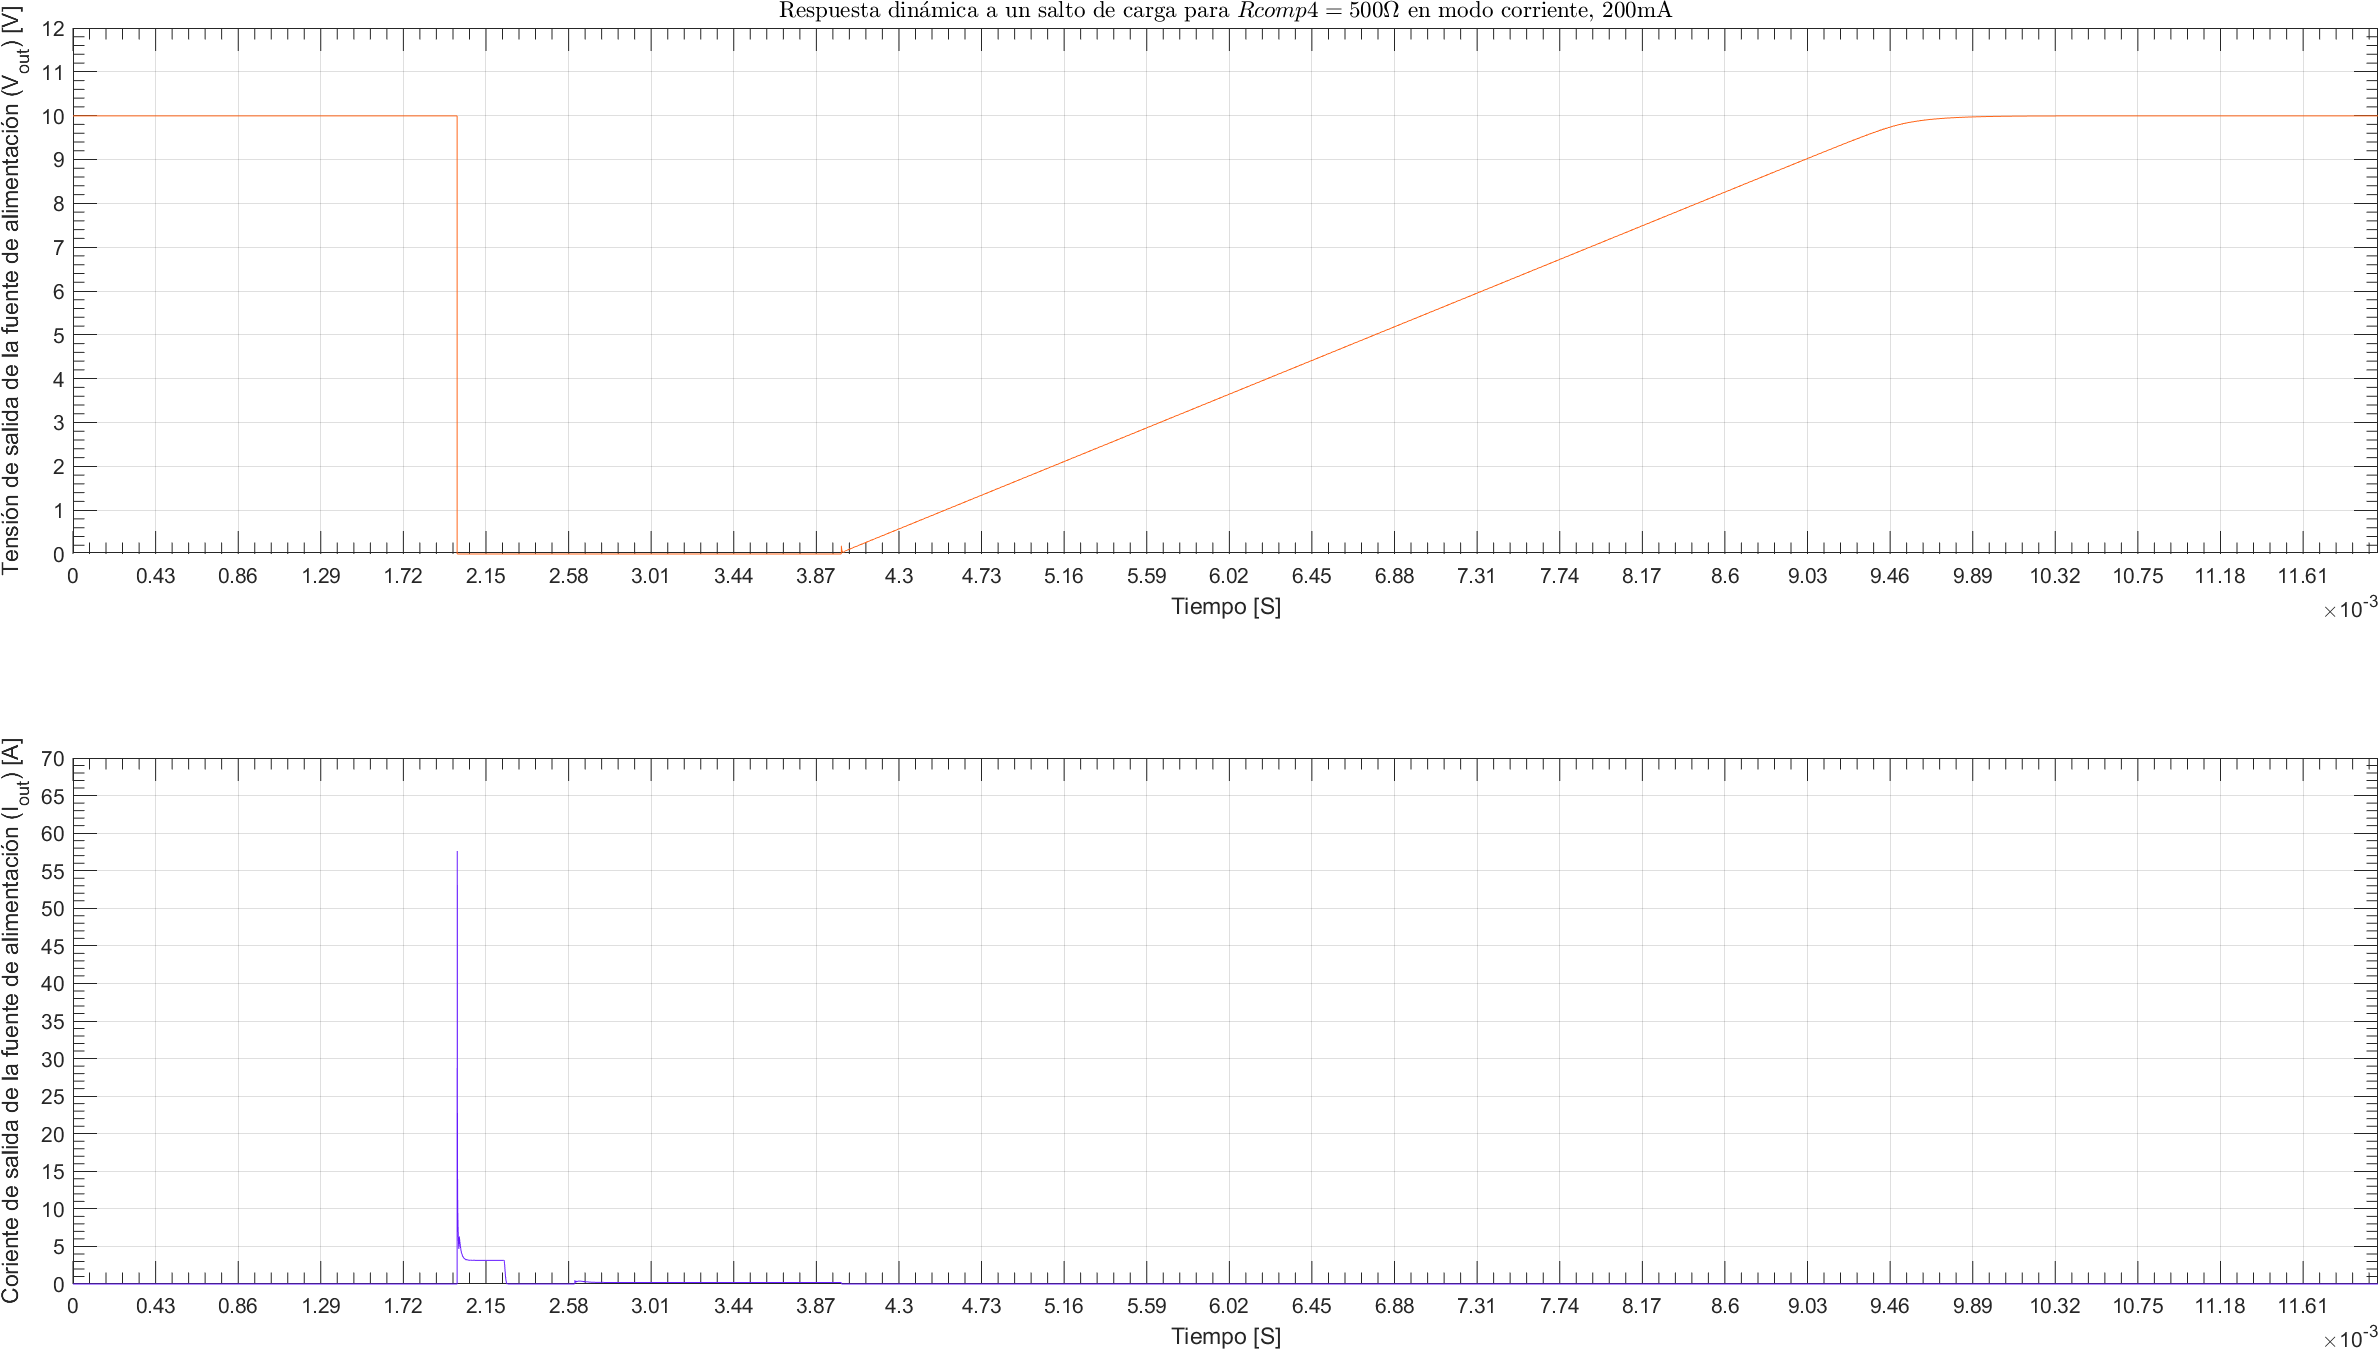
\includegraphics[width=1.1 \textwidth, angle=90]{./img/plots/dynamic/power_supply_RCOMP4_500_STEP_Modo4.png}
\caption{\label{fig:fig_power_supply_RCOMP4_STEP_500_Modo4}\footnotesize{Respuesta dinámica en modo corriente, $I_{out} = 200 \si[per-mode=symbol]{\milli\ampere}$, para $R_{comp_{4}} = 500 \si[per-mode=symbol]{\ohm} $.}}
\end{center}
\end{figure}

\clearpage

\begin{figure}[H] %htb
\begin{center}
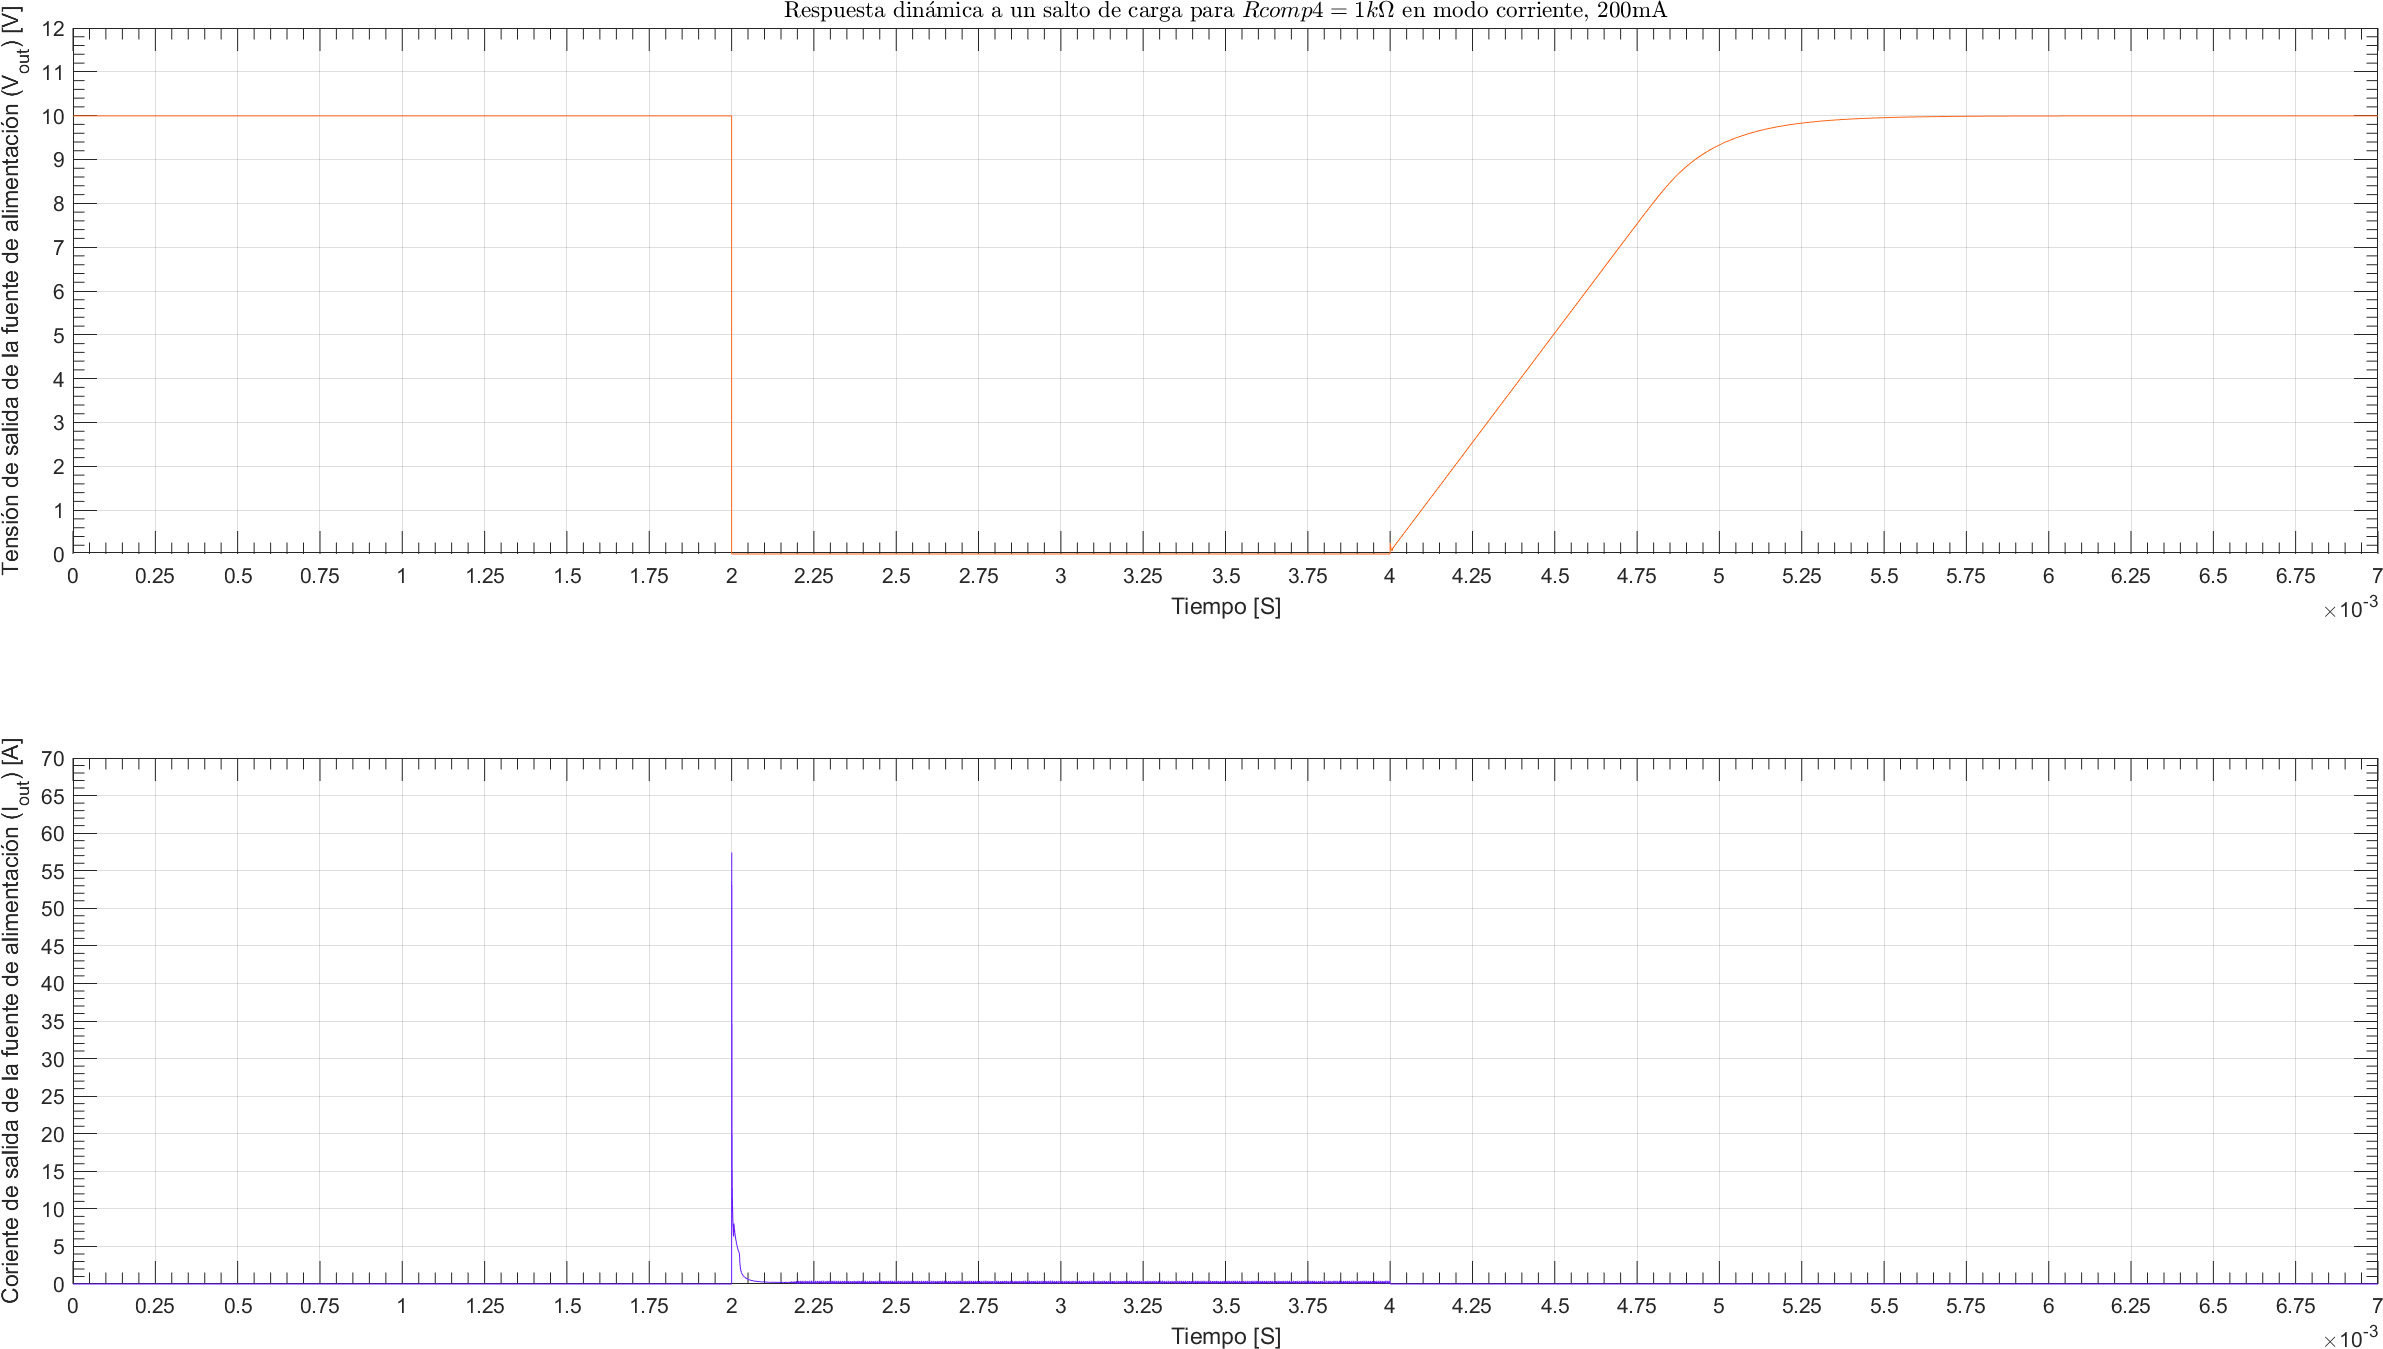
\includegraphics[width=1.1 \textwidth, angle=90]{./img/plots/dynamic/power_supply_RCOMP4_1k_STEP_Modo4.png}
\caption{\label{fig:fig_power_supply_RCOMP4_STEP_1k_Modo4}\footnotesize{Respuesta dinámica en modo corriente, $I_{out} = 200 \si[per-mode=symbol]{\milli\ampere}$, para $R_{comp_{4}} = 1 \si[per-mode=symbol]{\kilo\ohm} $.}}
\end{center}
\end{figure}

\clearpage

\begin{figure}[H] %htb
\begin{center}
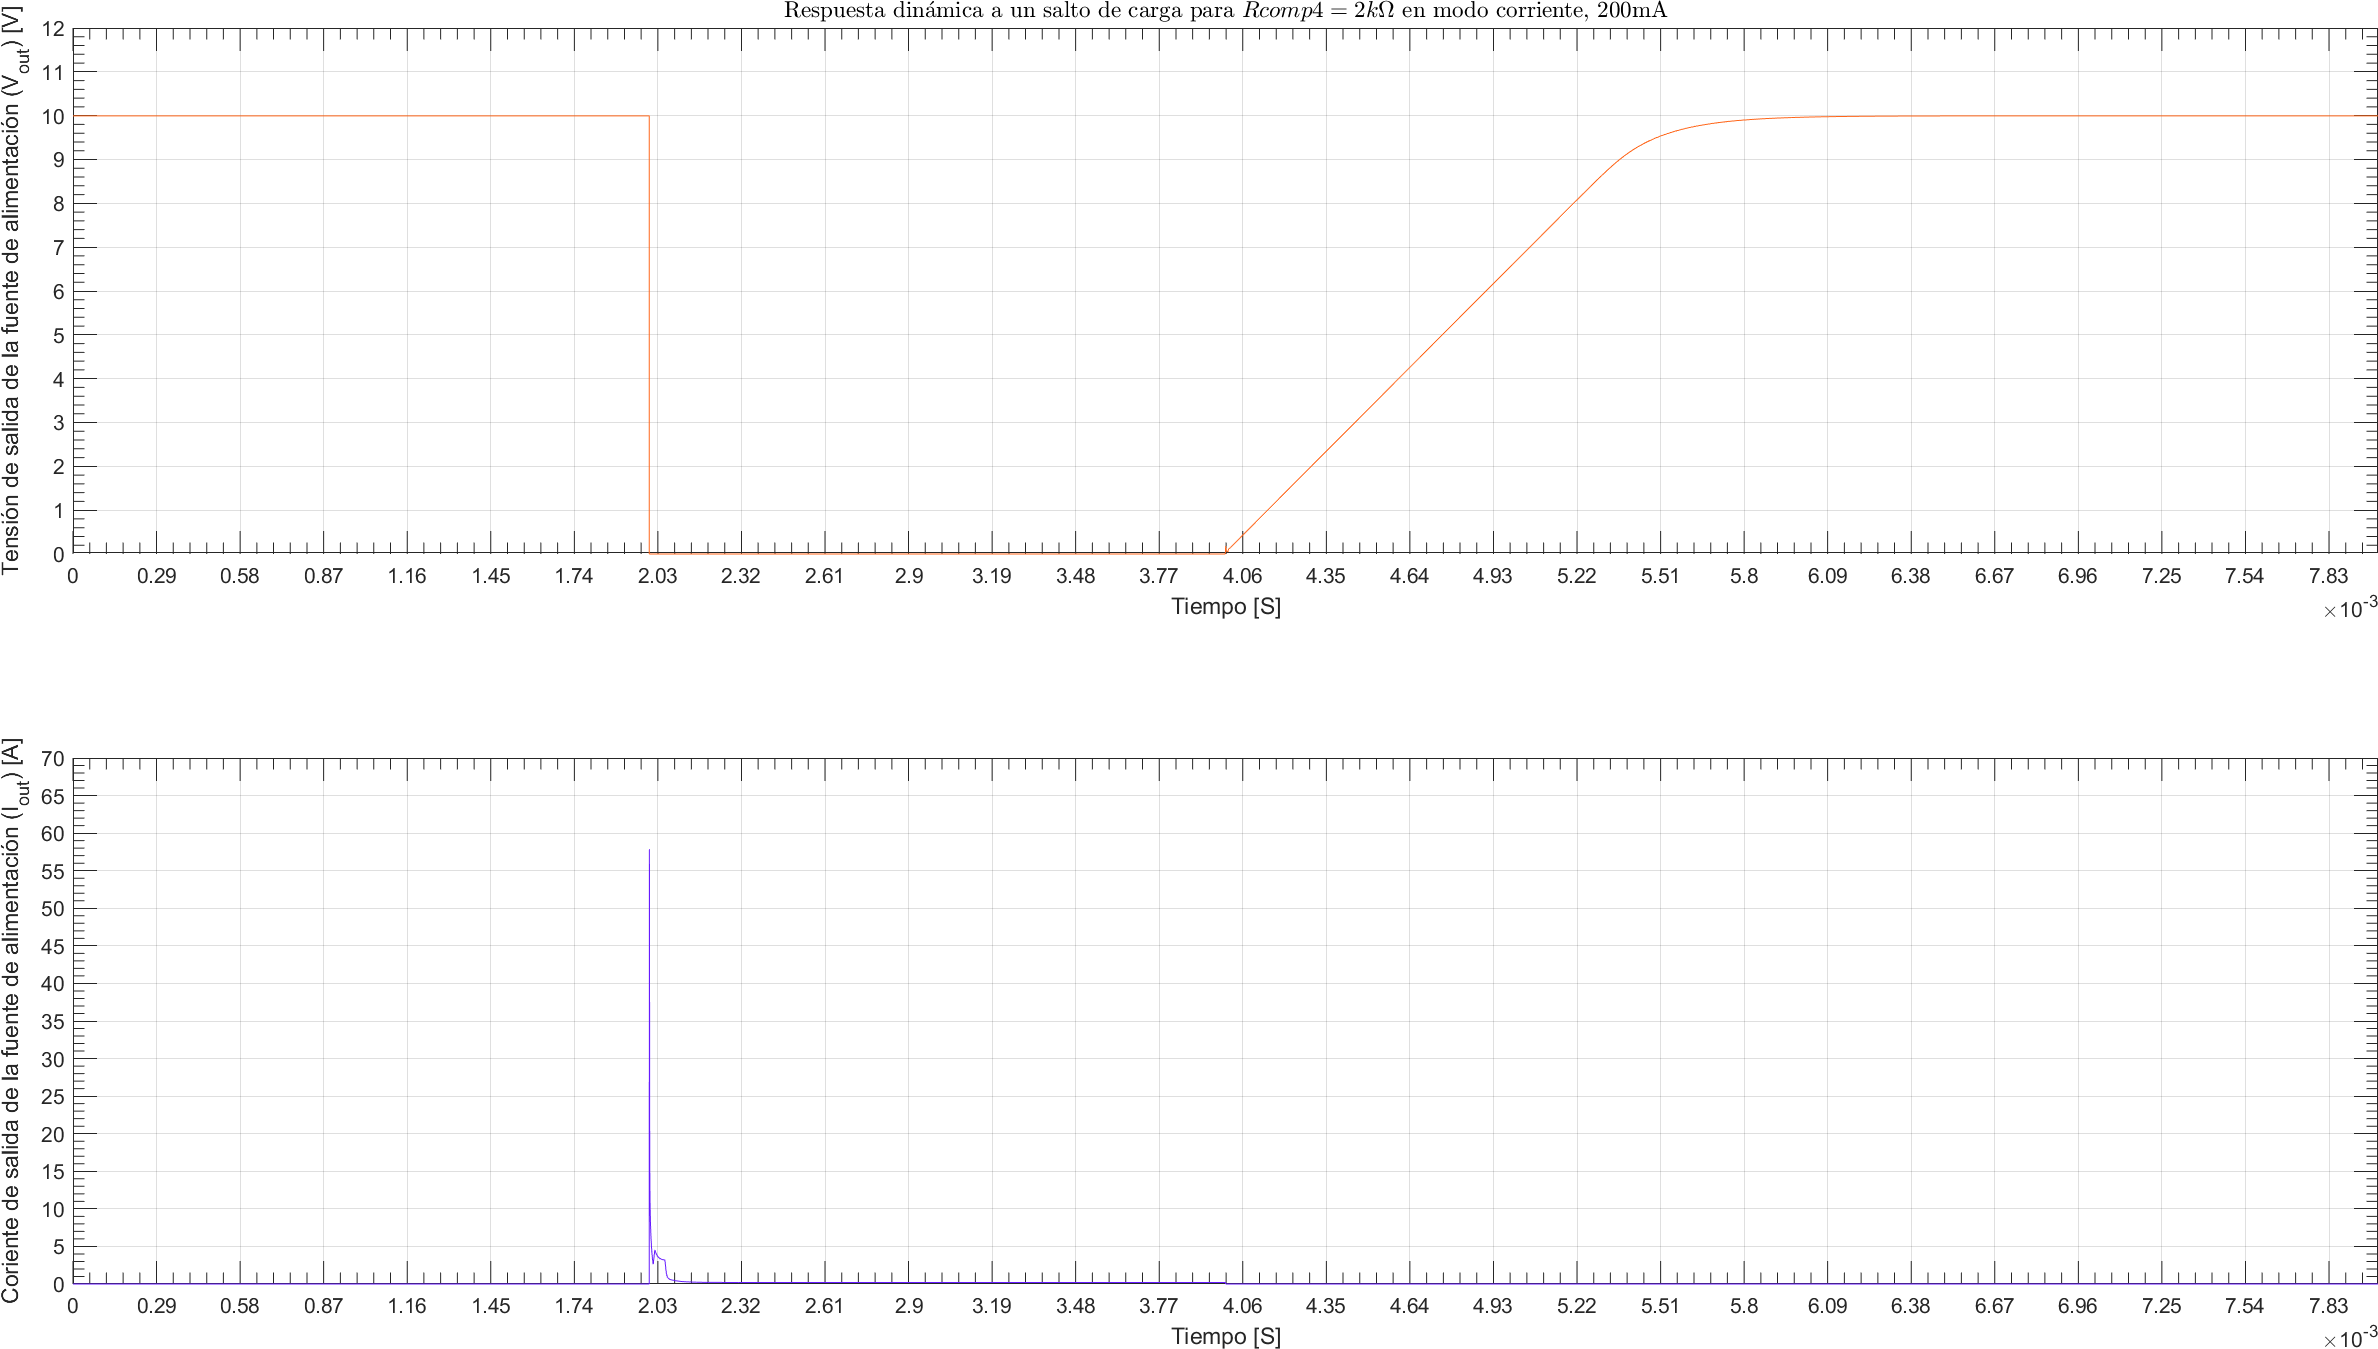
\includegraphics[width=1.1 \textwidth, angle=90]{./img/plots/dynamic/power_supply_RCOMP4_2k_STEP_Modo4.png}
\caption{\label{fig:fig_power_supply_RCOMP4_STEP_2k_Modo4}\footnotesize{Respuesta dinámica en modo corriente, $I_{out} = 200 \si[per-mode=symbol]{\milli\ampere}$, para $R_{comp_{4}} = 2 \si[per-mode=symbol]{\kilo\ohm} $.}}
\end{center}
\end{figure}

\clearpage







\clearpage
%\\\\\\\\\\\\\\\\\\\\\\\\\\\


%\\\\\\\\\\\\\\\\\\\\\\\\\\\
\subsection{Red de compensación de $C_{amort}/R_{amort}$}

La red formada por $\bm{R_{amort}}$ y $\bm{R_{amort}}$ actúa solo para el lazo de tensión, por lo que se analiza solo este modo.


\subsubsection{Análisis para $C_{amort}$ en modo tensión, $V_{out} = 10 \si[per-mode=symbol]{\volt}$, $R_{L} = 10 \si[per-mode=symbol]{\ohm}$}

Puede verse en las simulaciones que para una carga de $1 \si[per-mode=symbol]{\ampere} $ para $V_{out} = 10 \si[per-mode=symbol]{\volt}$ que con $C_{amort} = 10 \si[per-mode=symbol]{\micro\farad} $ o $C_{amort} = 22 \si[per-mode=symbol]{\micro\farad} $ mejora notablemente la respuesta dinámica del sistema, disminuyendo los sobre-picos de tensión y corriente, ver figura~\figref{fig:fig_power_supply_CAMORT_STEP_0_Modo1}, figura~\figref{fig:fig_power_supply_CAMORT_STEP_10u_Modo1} y figura~\figref{fig:fig_power_supply_CAMORT_STEP_22u_Modo1}, pero es de resaltar que en la ganancia de lazo empeora el margen de fase con el agregado del capacitor, ver la figura~\figref{fig:fig_power_supply_CAMORT_LOOP_Modo1}, no pudiéndose notar diferencia entre $C_{amort} = 10 \si[per-mode=symbol]{\micro\farad} $ y $C_{amort} = 22 \si[per-mode=symbol]{\micro\farad} $.

\vfill


% CAMORT MODO 1.

\clearpage

\begin{figure}[H] %htb
\begin{center}
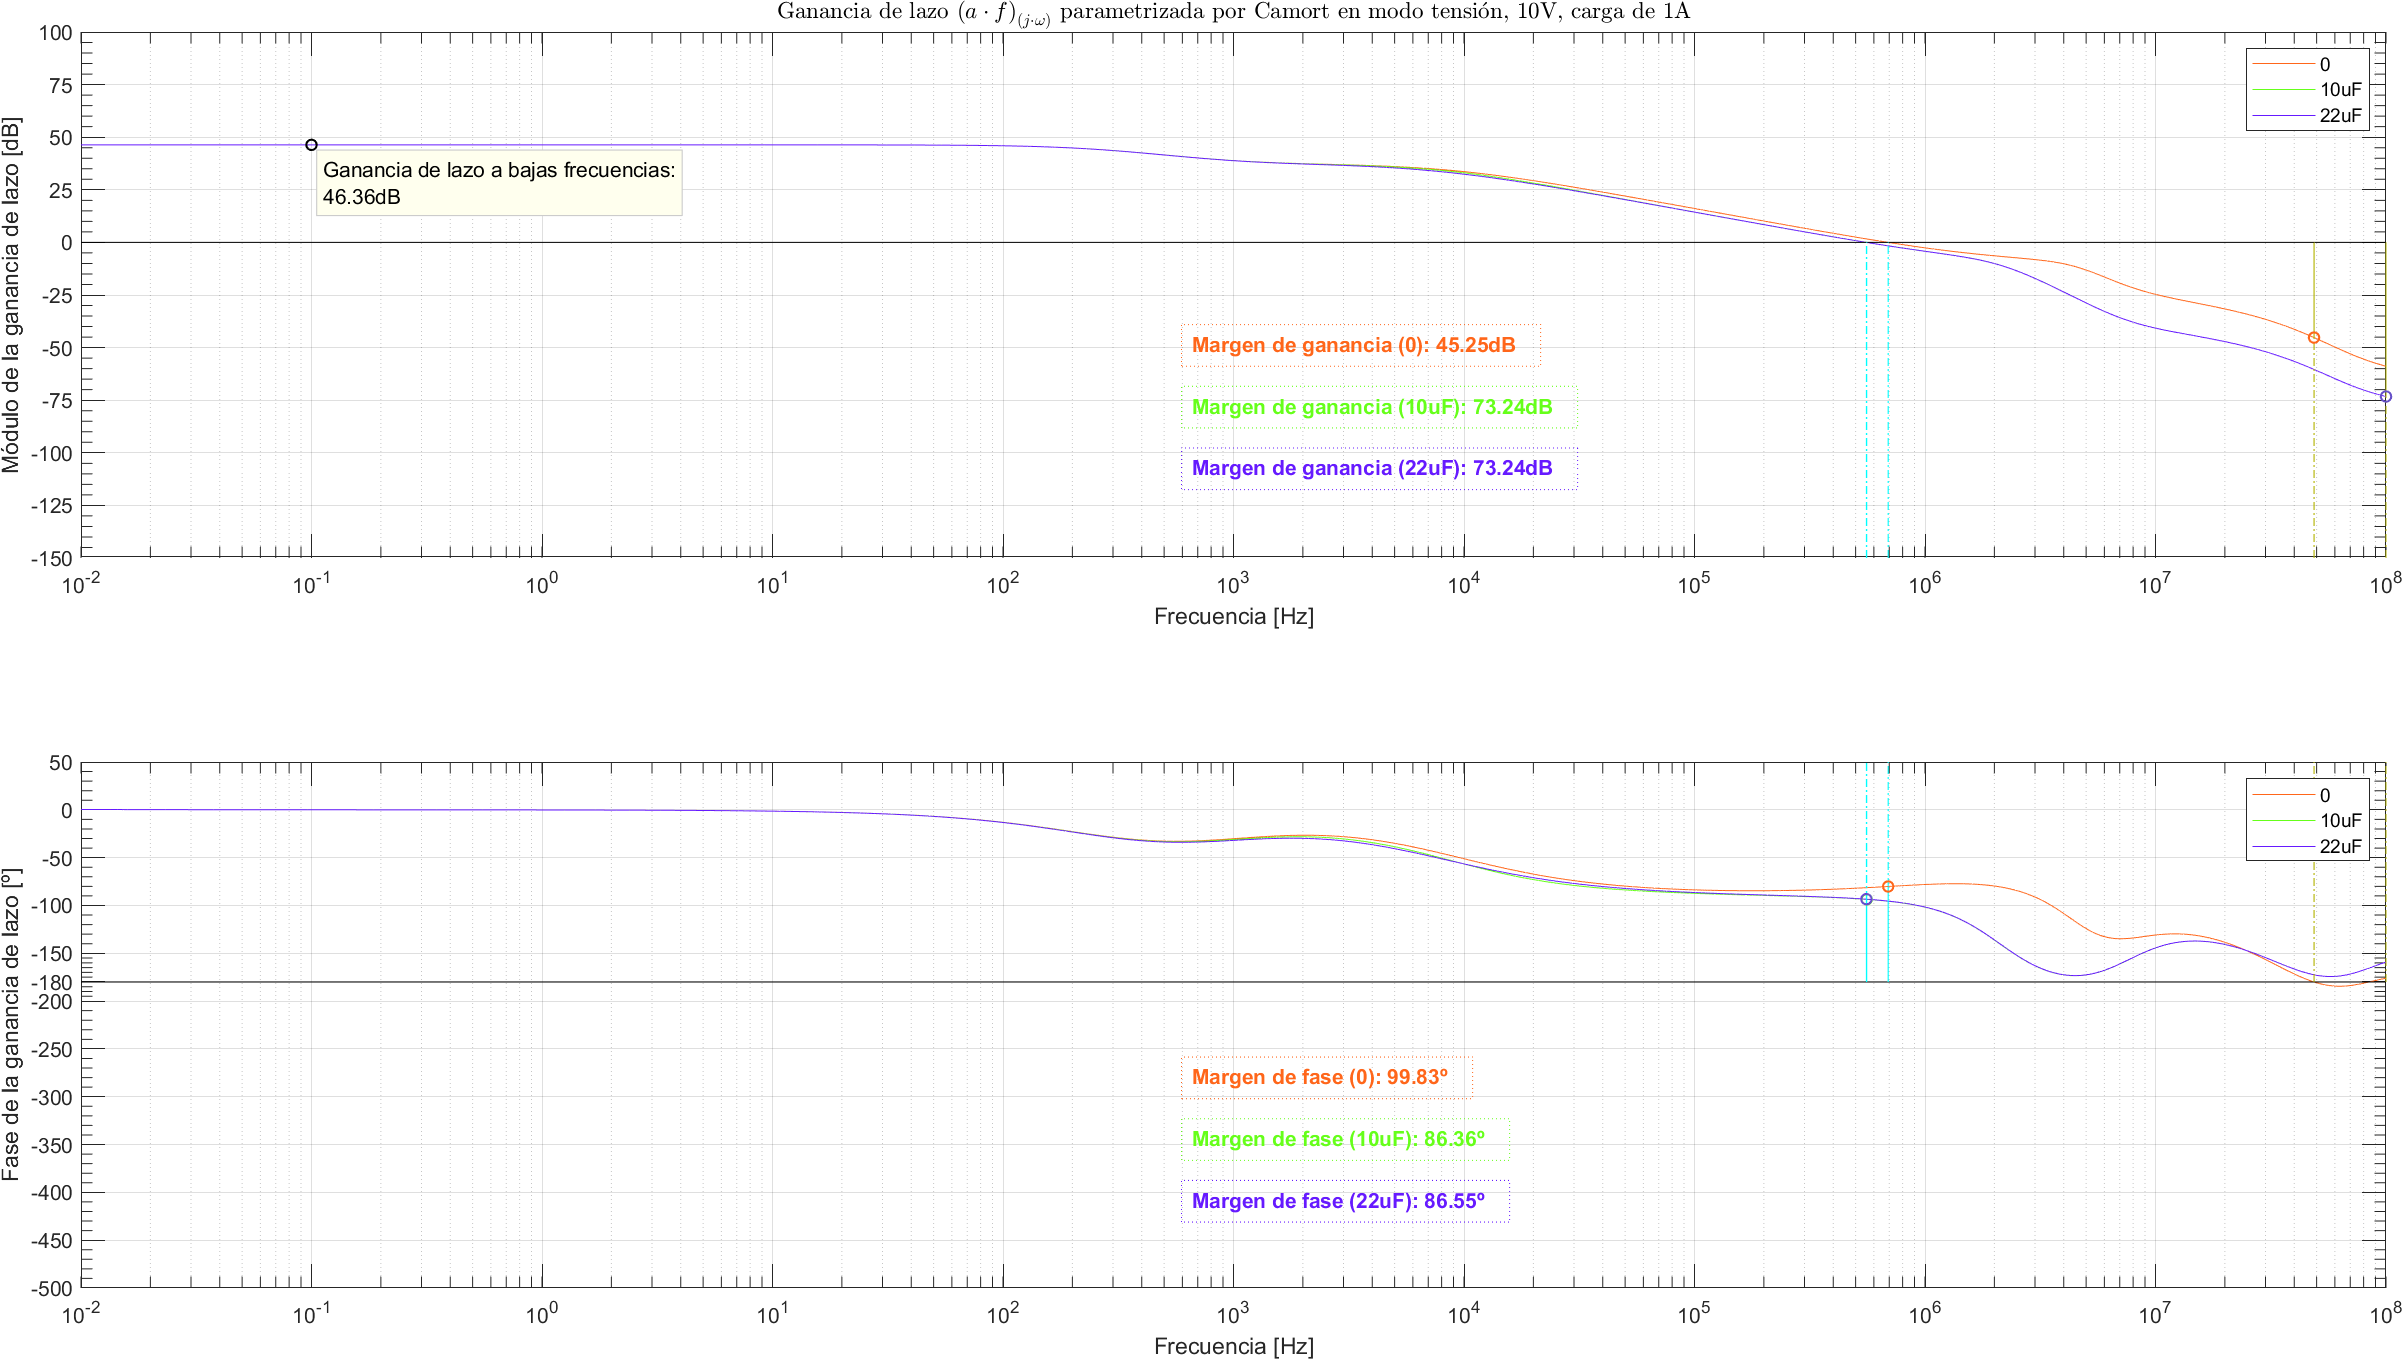
\includegraphics[width=1.1 \textwidth, angle=90]{./img/plots/loop/power_supply_CAMORT_LOOP_Modo1.png}
\caption{\label{fig:fig_power_supply_CAMORT_LOOP_Modo1}\footnotesize{Ganancia de lazo en modo tensión, $V_{out} = 10 \si[per-mode=symbol]{\volt}$, en función de la frecuencia parametrizada por $C_{amort}$.}}
\end{center}
\end{figure}


\clearpage

\begin{figure}[H] %htb
\begin{center}
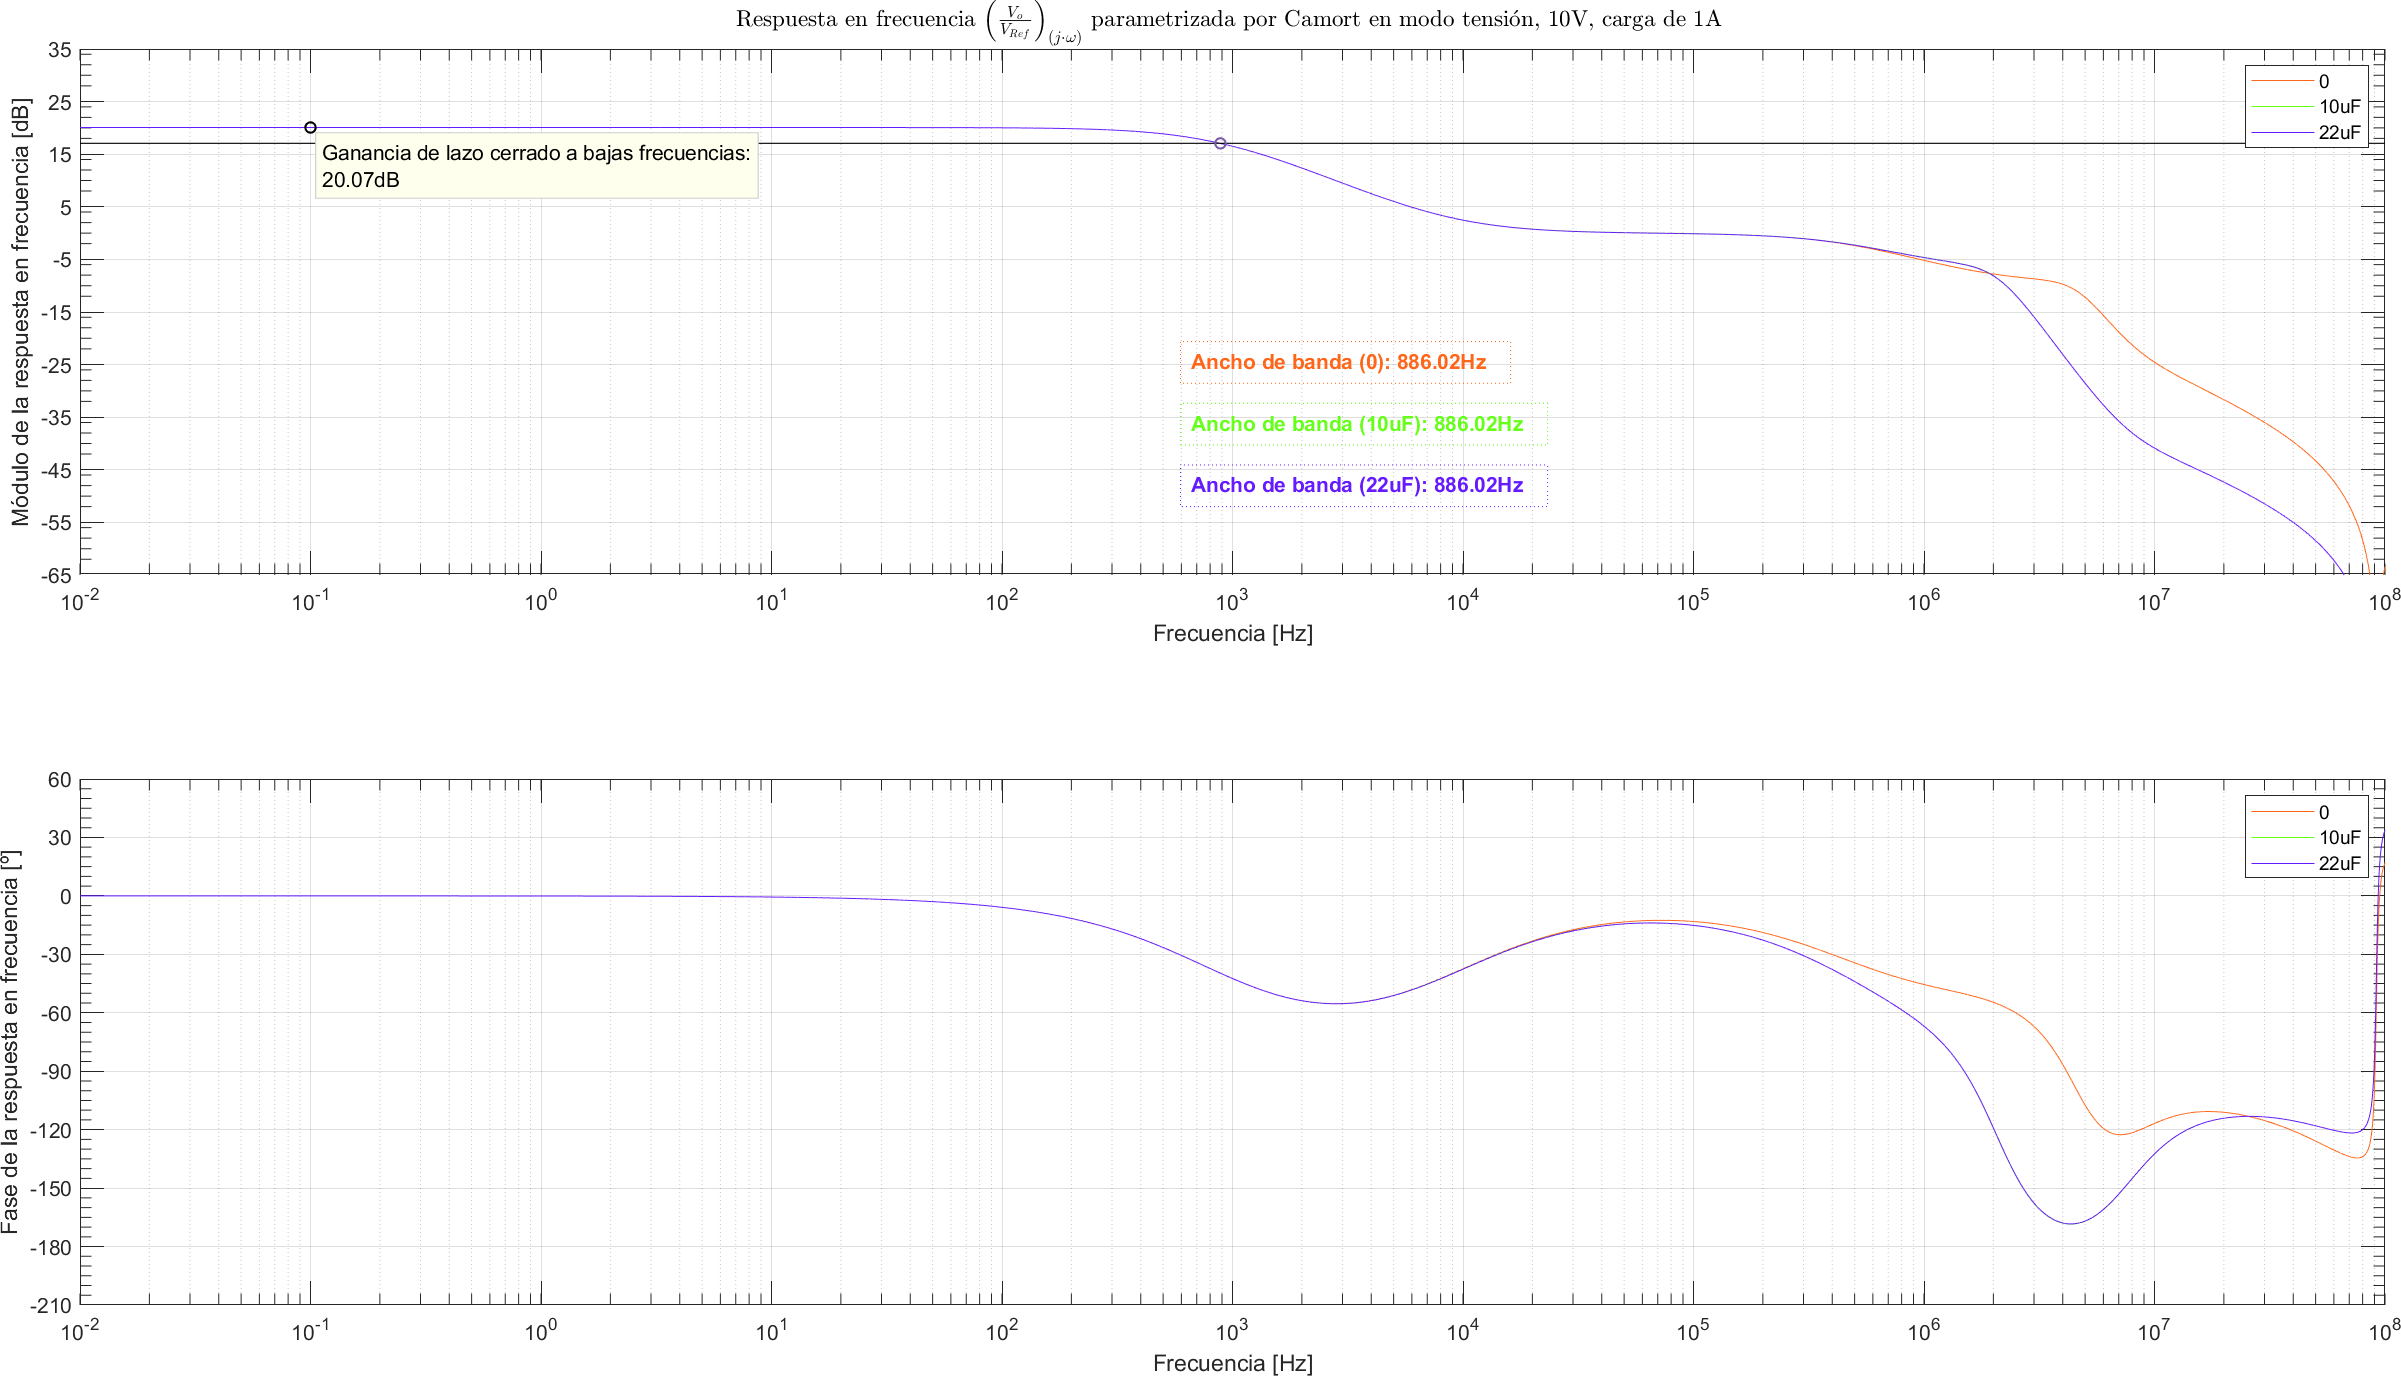
\includegraphics[width=1.1 \textwidth, angle=90]{./img/plots/rf/power_supply_CAMORT_RF_Modo1.png}
\caption{\label{fig:fig_power_supply_CAMORT_RF_Modo1}\footnotesize{Respuesta en frecuencia en modo tensión, $V_{out} = 10 \si[per-mode=symbol]{\volt}$, en función de la frecuencia parametrizada por $C_{amort}$.}}
\end{center}
\end{figure}

\clearpage

\begin{figure}[H] %htb
\begin{center}
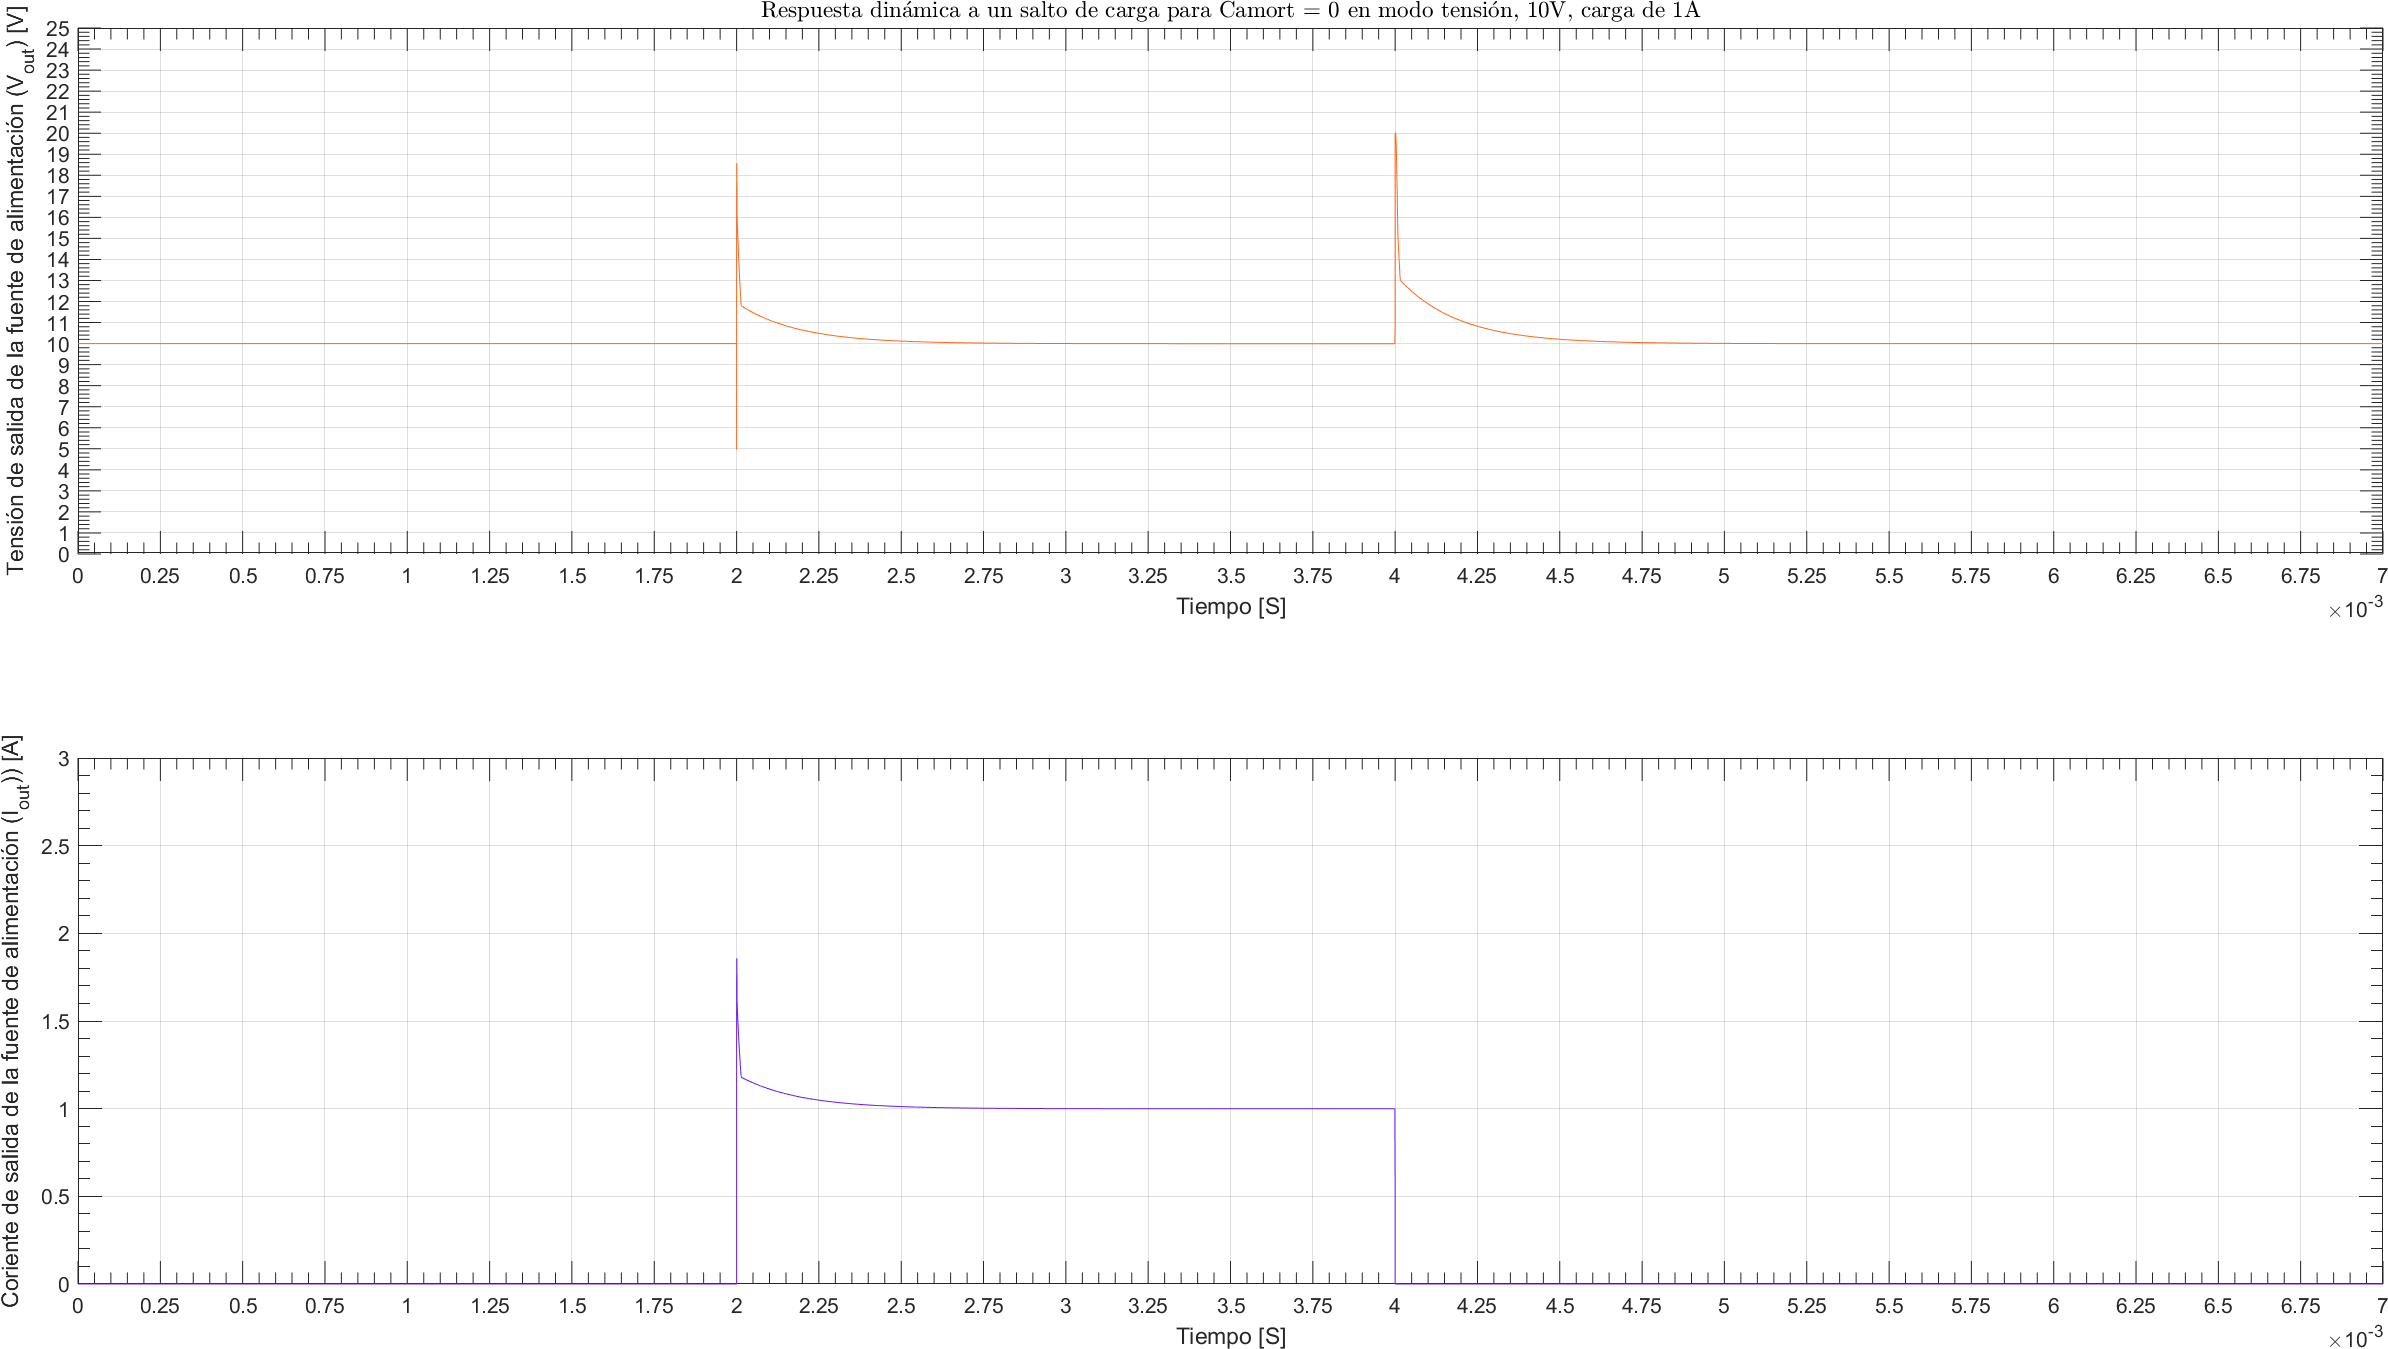
\includegraphics[width=1.1 \textwidth, angle=90]{./img/plots/dynamic/power_supply_CAMORT_0_STEP_Modo1.png}
\caption{\label{fig:fig_power_supply_CAMORT_STEP_0_Modo1}\footnotesize{Respuesta dinámica en modo tensión, $V_{out} = 10 \si[per-mode=symbol]{\volt}$, para $C_{amort} = 0 \si[per-mode=symbol]{\micro\farad} $.}}
\end{center}
\end{figure}

\clearpage

\begin{figure}[H] %htb
\begin{center}
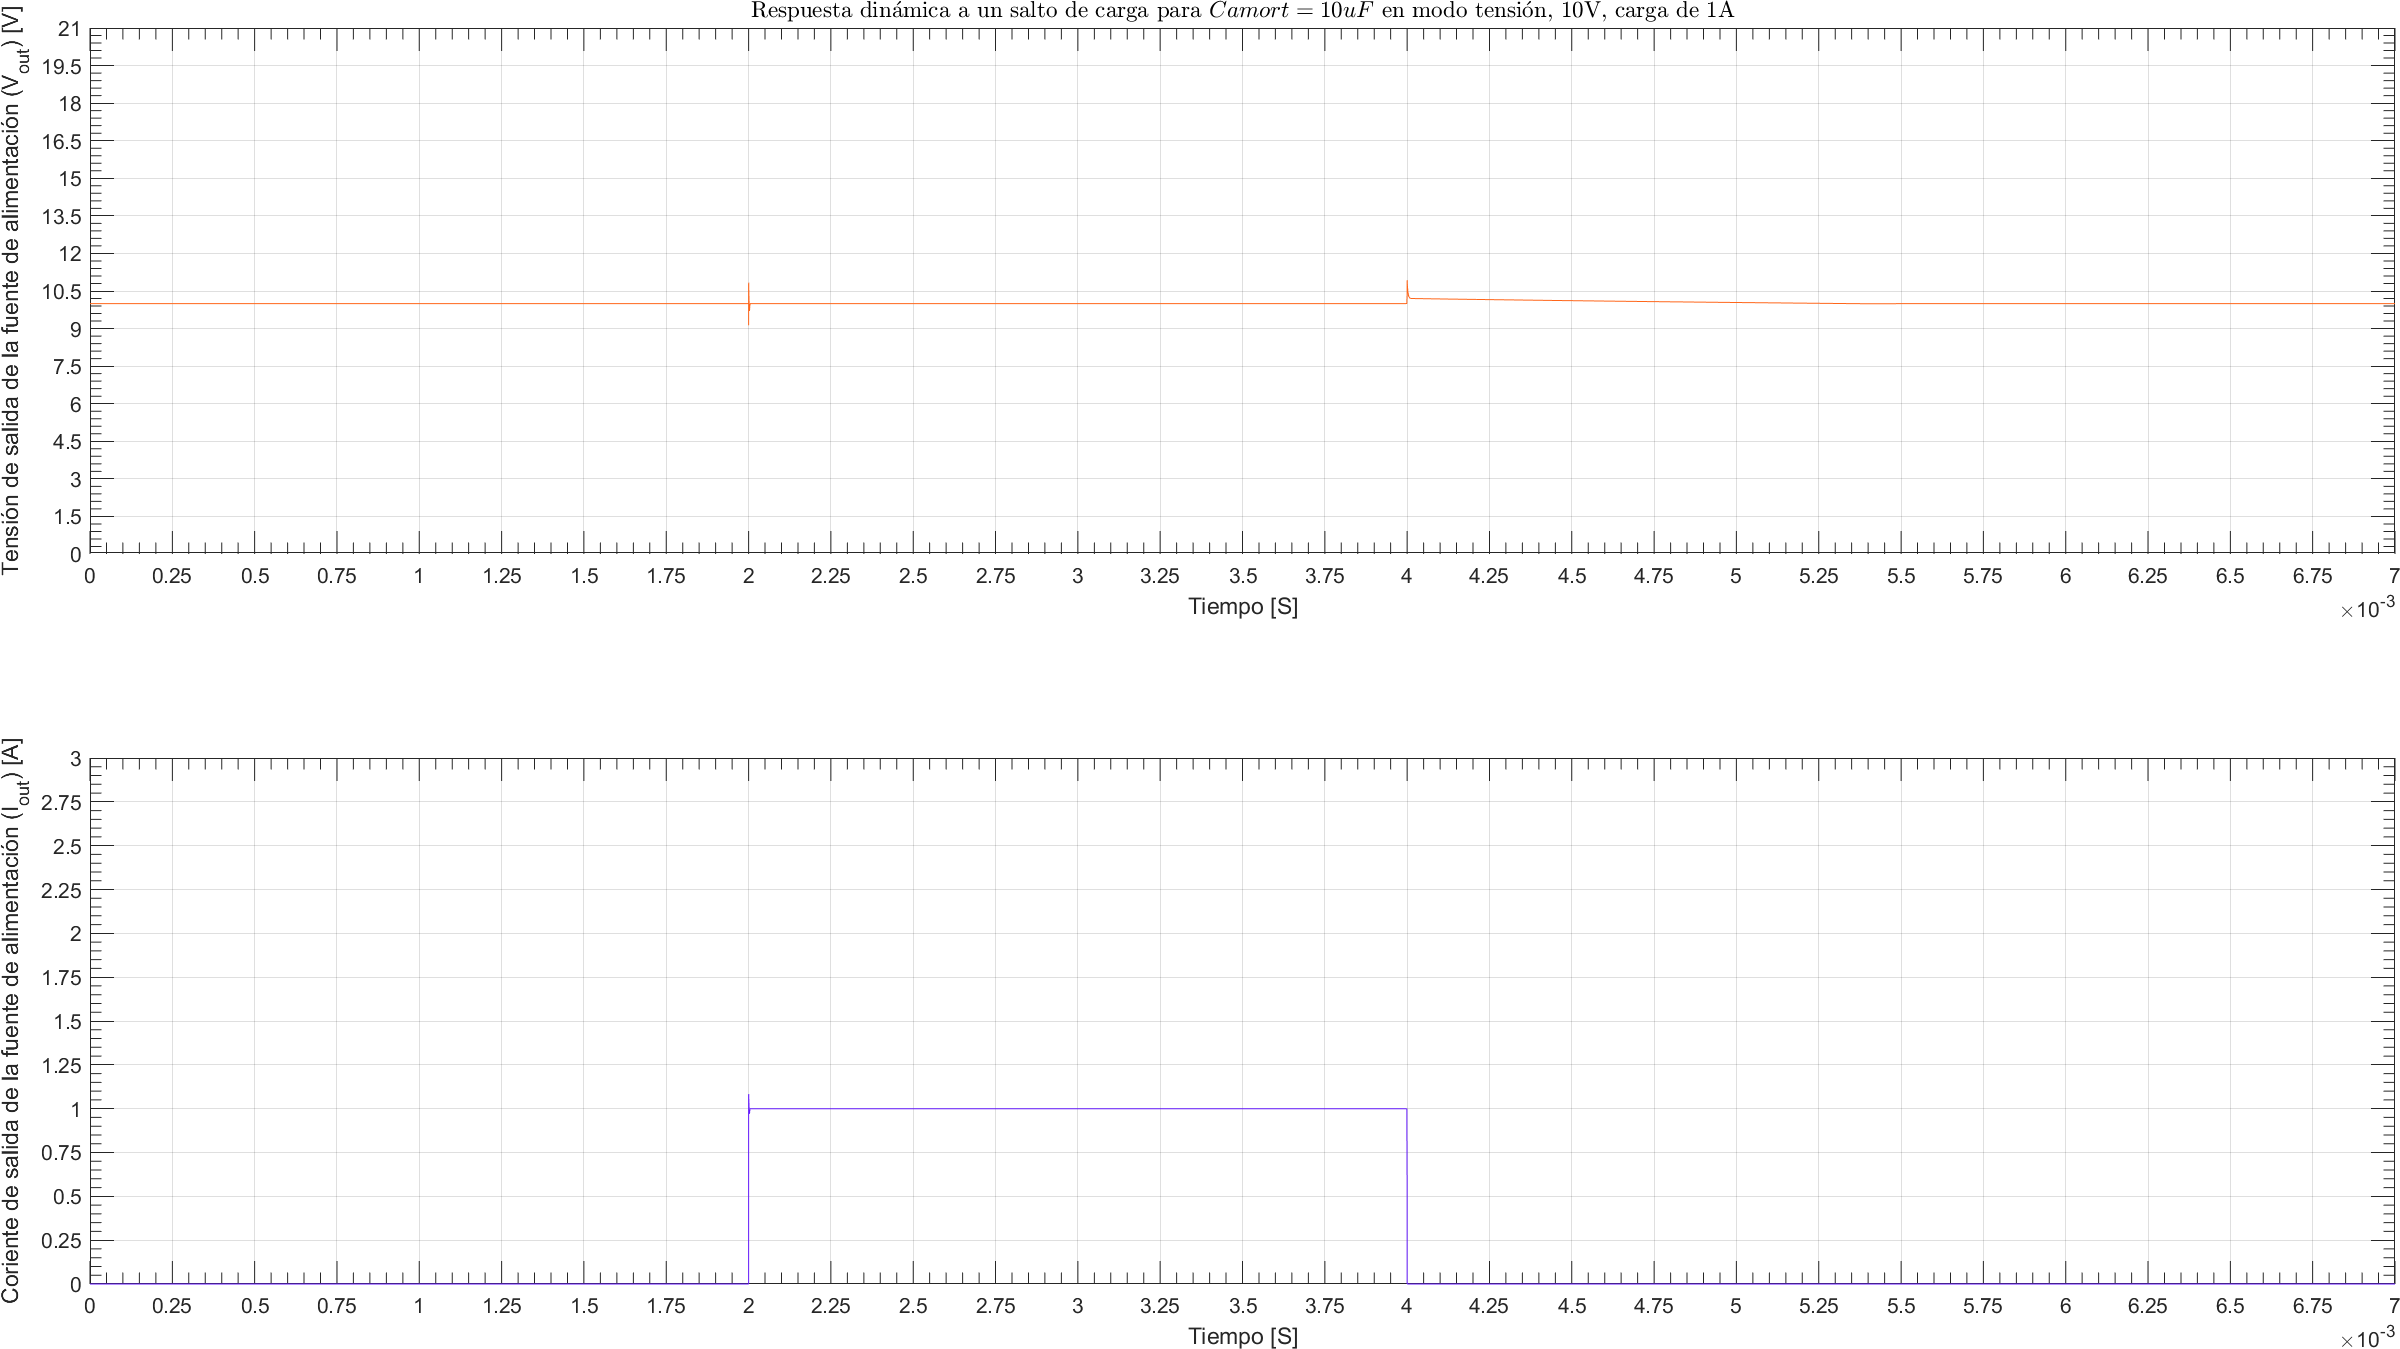
\includegraphics[width=1.1 \textwidth, angle=90]{./img/plots/dynamic/power_supply_CAMORT_10u_STEP_Modo1.png}
\caption{\label{fig:fig_power_supply_CAMORT_STEP_10u_Modo1}\footnotesize{Respuesta dinámica en modo tensión, $V_{out} = 10 \si[per-mode=symbol]{\volt}$, para $C_{amort} = 2 \si[per-mode=symbol]{\micro\farad} $.}}
\end{center}
\end{figure}

\clearpage

\begin{figure}[H] %htb
\begin{center}
\includegraphics[width=1.1 \textwidth, angle=90]{./img/plots/dynamic/power_supply_CAMORT_22u_STEP_Modo1.png}
\caption{\label{fig:fig_power_supply_CAMORT_STEP_22u_Modo1}\footnotesize{Respuesta dinámica en modo tensión, $V_{out} = 10 \si[per-mode=symbol]{\volt}$, para $C_{amort} = 5 \si[per-mode=symbol]{\micro\farad} $.}}
\end{center}
\end{figure}

\clearpage


\subsubsection{Análisis para $C_{amort}$ en modo tensión, $V_{out} = 1 \si[per-mode=symbol]{\volt}$, $R_{L} = 1 \si[per-mode=symbol]{\ohm}$}

Puede verse en las simulaciones que para una carga de $1 \si[per-mode=symbol]{\ampere} $ para $V_{out} = 1 \si[per-mode=symbol]{\volt}$ ocurre lo mismo que en el caso anterior prácticamente sin cambios.

\vfill


% CAMORT MODO 2.

\clearpage

\begin{figure}[H] %htb
\begin{center}
\includegraphics[width=1.1 \textwidth, angle=90]{./img/plots/loop/power_supply_CAMORT_LOOP_Modo2.png}
\caption{\label{fig:fig_power_supply_CAMORT_LOOP_Modo2}\footnotesize{Ganancia de lazo en modo tensión, $V_{out} = 1 \si[per-mode=symbol]{\volt}$, en función de la frecuencia parametrizada por $C_{amort}$.}}
\end{center}
\end{figure}


\clearpage

\begin{figure}[H] %htb
\begin{center}
\includegraphics[width=1.1 \textwidth, angle=90]{./img/plots/rf/power_supply_CAMORT_RF_Modo2.png}
\caption{\label{fig:fig_power_supply_CAMORT_RF_Modo2}\footnotesize{Respuesta en frecuencia en modo tensión, $V_{out} = 1 \si[per-mode=symbol]{\volt}$, en función de la frecuencia parametrizada por $C_{amort}$.}}
\end{center}
\end{figure}

\clearpage

\begin{figure}[H] %htb
\begin{center}
\includegraphics[width=1.1 \textwidth, angle=90]{./img/plots/dynamic/power_supply_CAMORT_0_STEP_Modo2.png}
\caption{\label{fig:fig_power_supply_CAMORT_STEP_0_Modo2}\footnotesize{Respuesta dinámica en modo tensión, $V_{out} = 1 \si[per-mode=symbol]{\volt}$, para $C_{amort} = 0 \si[per-mode=symbol]{\micro\farad} $.}}
\end{center}
\end{figure}

\clearpage

\begin{figure}[H] %htb
\begin{center}
\includegraphics[width=1.1 \textwidth, angle=90]{./img/plots/dynamic/power_supply_CAMORT_10u_STEP_Modo2.png}
\caption{\label{fig:fig_power_supply_CAMORT_STEP_10u_Modo2}\footnotesize{Respuesta dinámica en modo tensión, $V_{out} = 1 \si[per-mode=symbol]{\volt}$, para $C_{amort} = 2 \si[per-mode=symbol]{\micro\farad} $.}}
\end{center}
\end{figure}

\clearpage

\begin{figure}[H] %htb
\begin{center}
\includegraphics[width=1.1 \textwidth, angle=90]{./img/plots/dynamic/power_supply_CAMORT_22u_STEP_Modo2.png}
\caption{\label{fig:fig_power_supply_CAMORT_STEP_22u_Modo2}\footnotesize{Respuesta dinámica en modo tensión, $V_{out} = 1 \si[per-mode=symbol]{\volt}$, para $C_{amort} = 5 \si[per-mode=symbol]{\micro\farad} $.}}
\end{center}
\end{figure}

\clearpage




\subsubsection{Análisis para $R_{amort}$ en modo tensión, $V_{out} = 10 \si[per-mode=symbol]{\volt}$, $R_{L} = 10 \si[per-mode=symbol]{\ohm}$}

En el gráfico de ganancia de lazo para $R_{amort} = 0 \si[per-mode=symbol]{\ohm} $ se ve que el margen de ganancia es $0.04 \si[per-mode=symbol]{\decibel} $ y el margen de fase es $0.09 \si[per-mode=symbol]{\degree} $ muy cercanas a la condición de oscilación  y en el gráfico de respuesta transitoria para $R_{amort} = 0 \si[per-mode=symbol]{\ohm} $ se ve como el sistema tiene una oscilación muy pequeña una vez que se alcanza la tensión del escalón y se mantiene hasta finalizar este, ya que no hay elemento disipativo, en cambio con $R_{amort} = 1 \si[per-mode=symbol]{\ohm} $ o $R_{amort} = 5 \si[per-mode=symbol]{\ohm} $, la respuesta transitoria ya no oscila, mejorándose ampliamente los márgenes de fase y ganancia.




% RAMORT MODO 1.

\clearpage

\begin{figure}[H] %htb
\begin{center}
\includegraphics[width=1.1 \textwidth, angle=90]{./img/plots/loop/power_supply_RAMORT_LOOP_Modo1.png}
\caption{\label{fig:fig_power_supply_RAMORT_LOOP_Modo1}\footnotesize{Ganancia de lazo en modo tensión, $V_{out} = 10 \si[per-mode=symbol]{\volt}$, en función de la frecuencia parametrizada por $R_{amort}$.}}
\end{center}
\end{figure}


\clearpage

\begin{figure}[H] %htb
\begin{center}
\includegraphics[width=1.1 \textwidth, angle=90]{./img/plots/rf/power_supply_RAMORT_RF_Modo1.png}
\caption{\label{fig:fig_power_supply_RAMORT_RF_Modo1}\footnotesize{Respuesta en frecuencia en modo tensión, $V_{out} = 10 \si[per-mode=symbol]{\volt}$, en función de la frecuencia parametrizada por $R_{amort}$.}}
\end{center}
\end{figure}

\clearpage

\begin{figure}[H] %htb
\begin{center}
\includegraphics[width=1.1 \textwidth, angle=90]{./img/plots/dynamic/power_supply_RAMORT_0_STEP_Modo1.png}
\caption{\label{fig:fig_power_supply_RAMORT_STEP_0_Modo1}\footnotesize{Respuesta dinámica en modo tensión, $V_{out} = 10 \si[per-mode=symbol]{\volt}$, para $R_{amort} = 0 \si[per-mode=symbol]{\ohm} $.}}
\end{center}
\end{figure}

\clearpage

\begin{figure}[H] %htb
\begin{center}
\includegraphics[width=1.1 \textwidth, angle=90]{./img/plots/dynamic/power_supply_RAMORT_1_STEP_Modo1.png}
\caption{\label{fig:fig_power_supply_RAMORT_STEP_1_Modo1}\footnotesize{Respuesta dinámica en modo tensión, $V_{out} = 10 \si[per-mode=symbol]{\volt}$, para $R_{amort} = 1 \si[per-mode=symbol]{\ohm} $.}}
\end{center}
\end{figure}

\clearpage

\begin{figure}[H] %htb
\begin{center}
\includegraphics[width=1.1 \textwidth, angle=90]{./img/plots/dynamic/power_supply_RAMORT_5_STEP_Modo1.png}
\caption{\label{fig:fig_power_supply_RAMORT_STEP_5_Modo1}\footnotesize{Respuesta dinámica en modo tensión, $V_{out} = 10 \si[per-mode=symbol]{\volt}$, para $R_{amort} = 5 \si[per-mode=symbol]{\ohm} $.}}
\end{center}
\end{figure}

\clearpage


\subsubsection{Análisis para $R_{amort}$ en modo tensión, $V_{out} = 1 \si[per-mode=symbol]{\volt}$, $R_{L} = 1 \si[per-mode=symbol]{\ohm}$}

En el gráfico de ganancia de lazo para $R_{amort} = 0 \si[per-mode=symbol]{\ohm} $ se ve que el margen de ganancia es $-0.5 \si[per-mode=symbol]{\decibel} $ y el margen de fase es $-1.4 \si[per-mode=symbol]{\degree} $ apenas excediendo  la condición de oscilación  y en el gráfico de respuesta transitoria para $R_{amort} = 0 \si[per-mode=symbol]{\ohm} $ se ve como el sistema tiene una oscilación bastante marcada  una vez que se alcanza la tensión del escalón y se mantiene hasta finalizar este, ya que no hay elemento disipativo, en cambio con $R_{amort} = 1 \si[per-mode=symbol]{\ohm} $ o $R_{amort} = 5 \si[per-mode=symbol]{\ohm} $, la respuesta transitoria ya no oscila, mejorándose ampliamente los márgenes de fase y ganancia.




% RAMORT MODO 2.

\clearpage

\begin{figure}[H] %htb
\begin{center}
\includegraphics[width=1.1 \textwidth, angle=90]{./img/plots/loop/power_supply_RAMORT_LOOP_Modo2.png}
\caption{\label{fig:fig_power_supply_RAMORT_LOOP_Modo2}\footnotesize{Ganancia de lazo en modo tensión, $V_{out} = 1 \si[per-mode=symbol]{\volt}$, en función de la frecuencia parametrizada por $R_{amort}$.}}
\end{center}
\end{figure}


\clearpage

\begin{figure}[H] %htb
\begin{center}
\includegraphics[width=1.1 \textwidth, angle=90]{./img/plots/rf/power_supply_RAMORT_RF_Modo2.png}
\caption{\label{fig:fig_power_supply_RAMORT_RF_Modo2}\footnotesize{Respuesta en frecuencia en modo tensión, $V_{out} = 1 \si[per-mode=symbol]{\volt}$, en función de la frecuencia parametrizada por $R_{amort}$.}}
\end{center}
\end{figure}

\clearpage

\begin{figure}[H] %htb
\begin{center}
\includegraphics[width=1.1 \textwidth, angle=90]{./img/plots/dynamic/power_supply_RAMORT_0_STEP_Modo2.png}
\caption{\label{fig:fig_power_supply_RAMORT_STEP_0_Modo2}\footnotesize{Respuesta dinámica en modo tensión, $V_{out} = 1 \si[per-mode=symbol]{\volt}$, para $R_{amort} = 0 \si[per-mode=symbol]{\ohm} $.}}
\end{center}
\end{figure}

\clearpage

\begin{figure}[H] %htb
\begin{center}
\includegraphics[width=1.1 \textwidth, angle=90]{./img/plots/dynamic/power_supply_RAMORT_1_STEP_Modo2.png}
\caption{\label{fig:fig_power_supply_RAMORT_STEP_1_Modo2}\footnotesize{Respuesta dinámica en modo tensión, $V_{out} = 1 \si[per-mode=symbol]{\volt}$, para $R_{amort} = 1 \si[per-mode=symbol]{\ohm} $.}}
\end{center}
\end{figure}

\clearpage

\begin{figure}[H] %htb
\begin{center}
\includegraphics[width=1.1 \textwidth, angle=90]{./img/plots/dynamic/power_supply_RAMORT_5_STEP_Modo2.png}
\caption{\label{fig:fig_power_supply_RAMORT_STEP_5_Modo2}\footnotesize{Respuesta dinámica en modo tensión, $V_{out} = 1 \si[per-mode=symbol]{\volt}$, para $R_{amort} = 5 \si[per-mode=symbol]{\ohm} $.}}
\end{center}
\end{figure}

\clearpage



\clearpage
%\\\\\\\\\\\\\\\\\\\\\\\\\\\



